\documentclass[11pt]{article}   	
\usepackage[utf8]{inputenc}
\usepackage{geometry}                		
\geometry{letterpaper, margin=1in}                   		
\usepackage{graphicx}			
\usepackage{amssymb}
\usepackage{setspace}
\usepackage{sectsty}
\clubpenalty = 10000
\widowpenalty = 10000
\usepackage[labelsep=period]{caption}
\captionsetup[table]{name=TABLE}
\usepackage[explicit]{titlesec}
\titleformat{\section}
  {\scshape\bfseries\centering}{\thesection}{1em}{\MakeUppercase{#1}}
\allsectionsfont{\normalsize}{\centering}
\renewcommand{\thetable}{\Roman{table}}
\usepackage{etoolbox}
\usepackage{relsize}
\usepackage{mathrsfs}  
\usepackage{array}
%\usepackage[fleqn]{amsmath}
%\setlength{\mathindent}{0pt}

\RequirePackage{lineno}
\linenumbers

%\AtBeginEnvironment{tabular}{\doublespacing}

\usepackage{morefloats}
\usepackage{hyperref}
\usepackage{caption}
\usepackage{slashed}

\hypersetup{
   colorlinks=true,
   linktoc=page,
   linkcolor=blue,
   citecolor=blue,
}



\begin{document}



\begin{center}

\textbf{Jet-Track Correlation Studies of the Quark Gluon Plasma}



\vspace{2.5 in}
BY

HALLIE CAUSEY TRAUGER

M.Ed. University of Illinois at Chicago, 2015

M.S. University of Illinois at Chicago, 2014

B.A. University of Chicago, 2010

\vspace{2.5 in}
THESIS

Submitted in partial fulfilment of the requirements 

for the degree of Doctor of Philosophy in Physics 

in the Graduate College of the University of Illinois at Chicago, 2017

\vspace{0.2 in}
Chicago, IL

\end{center}

\vspace{0.2 in}

DEFENSE COMMITTEE:

\setlength{\parindent}{0.5in} Olga Evdokimov, Chair and Advisor

David Hofman

Zhenyu Ye

Misha Stephanov

Julia Velkovska, Vanderbilt University


\pagenumbering{gobble} 



\clearpage{}

\pagenumbering{roman}
\setcounter{page}{2}
    
\section*{}
    
\vspace{2.5 in}
    
\textit{For my students, with the hope that they, too, may enjoy the privilege of following their curiosity and passions wherever these may lead.}
\clearpage

\section*{Acknowledgements}

Thanks go here...

\vspace{1in}

\begin{flushright}

HCT
\end{flushright}
\clearpage{}

\section*{Contribution of Authors}

- Note previous publications (HIN-14-016, HIN-15-011, HIN-16-020)

\noindent - Describe CMS authorship policy

\noindent - Outline general CMS inputs (reconstruction etc.) that contributed to work

\noindent - Outline aspects that are my own work (and others' contributions to these as well, esp. Run 2)

\clearpage

\setcounter{tocdepth}{2}
\tableofcontents
\clearpage{}

\listoftables
\clearpage{}

\listoffigures
\clearpage{}

\section*{List of Abreviations}

\begin{table}[htbp]

\begin{tabular}{l l}

BNL & Brookhaven National Laboratory\\

CERN & Conseil Europ\'{e}en pour la Recherche Nucl\'{e}aire\\

CMS & Compact Muon Solenoid \\

ECAL & Electromagnetic Calorimeter\\

$E_{\rm T}$ & Transverse Energy\\

HCAL & Hadronic Calorimeter\\

HF & Hadronic Forward\\

HLT & High Level Trigger \\ 

JEC & Jet Energy Correction\\

JES & Jet Energy Scale\\

JFF  & Jet Fragmentation Function \\

LHC & Large Hadron Collider \\

MC & Monte Carlo\\

PbPb & Lead-lead (collision data)\\

PDF & Parton Distribution Function\\

pPb & Proton-lead (collision data)\\

pp & Proton-proton (collision data)\\

pQCD & Perturbative Quantum Chromodynamics\\

$p_{\rm T}$ & Transverse Momentum\\

QCD & Quantum Chromodynamics\\

QGP  &  Quark Gluon Plasma \\

RHIC & Relativistic Heavy Ion Collider\\

UE & Underlying Event \\

\end{tabular}

\end{table}
\clearpage{}

\section*{Summary}
\input{Summary}
\clearpage{}


%MAIN MATTER

\pagenumbering{arabic}
\setcounter{page}{1}
\doublespacing


\section{Introduction}
\label{sec:Introduction}
\input{Introduction}
\clearpage

\section{The quark gluon plasma}
\label{sec:Theory}

\subsection{Predictions and early evidence for the quark gluon plasma}

Quantum chromodynamics (QCD) describes the interactions of the quarks and gluons (together known as partons) via the strong nuclear force.  The strength of the QCD interactions, described by the QCD coupling constant $\alpha_{s}(Q)$ decreases as distances between strongly interacting partons decreases and their exchanged momentum $Q$: 

\begin{equation}
\label{eq:alpha_s}
\alpha_{s}(Q) \propto \frac{1}{{\rm ln}(\frac{Q^{2}}{\Lambda_{QCD}})}, 
\end{equation}

\noindent where $\Lambda_{QCD} \approx 0.2$ GeV gives the QCD scale.  Figure~\ref{fig:alpha_s} shows the dependence of $\alpha_{s}$ on momentum scale $Q$.  In the regime where separations between partons are relatively large (small $Q$), $\alpha_{s}$ is large, leading to the observed confinement of quarks and gluons in composite particles called hadrons, most commonly baryons (comprised of 3 quarks, including protons and neutrons) and mesons (comprised of 2 quarks).  In the large $Q$ regime, however--accessed via large baryon chemical potential $\mu_{B}$ or large temperature $T$--the strength of the coupling constant $\alpha_{s}$ decreases, in a phenomenon known as asymptotic freedom.  Asymptotic freedom both permits the accurate approximation of high-energy hadron interactions using perturbation theory (pQCD), and implies the deconfinement of quarks and gluons.  This phase of deconfined quarks and gluons, known as the  quark gluon plasma (QGP), was originally conceived as a gas of color-charged quarks and gluons, analogous to the plasma of photons and electrons previously studied in quantum electrodynamics.  In collider studies, this suggests the possibility of a phase transition anticipated between the hadron gas phase present under ordinary matter conditions, and the QGP phase present at sufficiently great $\mu_{B}$ or $T$~\cite{Kalashnikov:1979, Shuryak:1980tp}.

\begin{figure}[h!]
\begin{center}
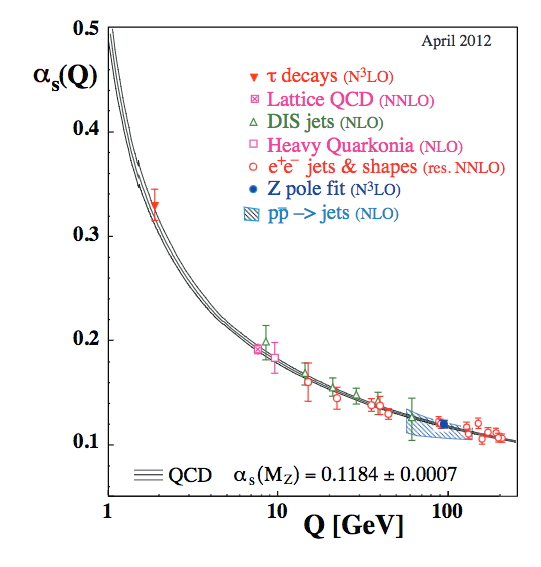
\includegraphics[width=0.6\textwidth]{figures/Theory/Alpha_s.png}
\caption[QCD coupling constant $\alpha_{s}$]{Momentum scale dependence of QCD coupling constant $\alpha_{s}$, from Ref.~\cite{Bethke:2012jm}.}
\label{fig:alpha_s}
\end{center}
\end{figure}


In the early 1980s, relativistic nuclear collisions were suggested as a means of producing sufficient temperatures and densities to induce a quark-gluon plasma and probe the transition between the QGP and ordinary matter.  Efforts were also made to anticipate key experimental signatures of the short-lived possible QGP, relying in many cases on the anticipation that the QGP would behave according to a hydrodynamic description of a system in at least partial thermal equilibrium.  Proposed signatures included enhancements of strange (heavy) quarks, unusual event structures, greater rates of direct dilepton and photon production~\cite{Bjorken:1983}.  The first heavy ion collisions began with fixed-target experiments at the Super Proton Synchrotron (SPS) at CERN in the mid-1980s, colliding nuclei including gold and lead at energies from 40 GeV to 160 GeV through the 1990s.  Analysis of the hadron yields in these collisions showed an apparent chemical equilibrium of quarks and gluons at about 170 MeV and enhancement (as anticipated) both of strangeness (via kaon/pion ratios, and J/$\psi$ production rates).  In the early 2000, a CERN press release cited these results in declaring that ``a common assessment of the collected data leads us to believe that a new state of matter has indeed been created...[that] features many of the characteristics of the theoretically predicted quark-gluon plasma''~\cite{Heinz:2000bk}.

Shortly after the SPS announcement, the first gold-gold collisions began at the Relativistic Heavy Ion Collider (RHIC) at Brookhaven National Laboratory, beginning an era of high-energy heavy ion collisions that would later be complimented by a parallel program at the Large Hadron Collider at CERN.  Through data collection and analysis by experiments at each of these colliders over the ensuing nearly two decades, the field has gradually shifted from searches for signatures of QGP formation in heavy ion collisions, to detailed characterizations of its properties and evolution.  In 2005, the four experimental collaborations at RHIC (BRAHAMS, PHENIX, PHOBOS, and STAR) published coordinated white papers~\cite{Arsene:2004fa, Adcox:2004mh, Back:2004je, Adams:2005dq} summarizing the assembled evidence that results from  gold-gold collisions could not be explained by models of ordinary hadronic matter--most notably in signatures of collective behavior (see Sec.~\ref{sec:theory_collectivity}) and in suppression of particles with relatively high transverse momentum (see Sec.~\ref{sec:theory_jets}).  Beginning in 2010, heavy ion studies at the LHC by the ALICE, ATLAS, and CMS Collaborations (and more recently by the LHCb Collaboration) have complimented the RHIC access to a wide range of center-of-mass-energies in the 7.7 GeV to 200 GeV range with measurements at 2.76 TeV and 5.02 TeV.

\subsection{Properties of the quark gluon plasma}

-- Temperature and energy density at RHIC and LHC energies

-- Time-evolution (initial conditions, hydrodynamic expansion of the QGP, hadronization)

-- QCD phase diagram characterization

\subsection{Characterizing collision centrality}
\label{sec:glauber}

-- Glauber model

***** GLAUBER DIAGRAM *****

-- TAA

-- Glauber limitations

-- Experimental definitions of centrality


\subsection{Collective behavior in the QGP}
\label{sec:theory_collectivity}

-- Flow and interpretations (including harmonic decomp. examples)

-- Hydro

-- IS fluctuations

***** DIAGRAM OF IS CONFIGURATIONS AND CONNECTION TO HARMONICS******

\clearpage

\section{Jets as probes of the quark gluon plasma}
\label{sec:theory_jets}

Hard scatterings in heavy ion collisions can provide powerful $in situ$ probes of the quark gluon plasma.  Because of asymptotic freedom, high-energy parton-parton processes can be accurately characterized via pQCD, and have been thoroughly studied experimentally in hadron-hadron collisions.  In heavy ion collisions, the initial parton-parton interaction should by 
causality behave the same as a parton-parton interaction in hadron-hadron collisions.  After the collision, however, outgoing partons traverse the quark gluon plasma, providing the opportunity to study medium properties by comparing heavy ion results to expectations inferred from hadron-hadron ``vacuum'' reference data.  These studies are facilitated by the ``factorization theorem'' in pQCD, which states that the cross section $\sigma_{AB\rightarrow h}^{\rm hard}$ of hadron $h$  produced in the hard process $ A + B \rightarrow h$) can be decomposed into contributions from:  

\begin{itemize}
\item The perturbative cross section of the parton hard scattering $\sigma_{ab\rightarrow c}^{\rm hard}$ 
\item The initial parton distribution functions (PDFs) of partons in the colliding nuclei A and B ($f_{a/A}$ and $f_{b/B}$ for partons of flavor $a$ and $b$)
\item The fragmentation function $\mathscr{D}_{c\rightarrow h}$ describing the probability that parton $c$ fragments into hadron h with momentum fraction $z = p_{h}/p_{c}$ 
\end{itemize}

\noindent The total cross section may be represented, schematically, as:  

\begin{equation}
\label{eq:factorization}
d \sigma_{AB\rightarrow h}^{\rm hard} = f_{a/A}(x_{a},Q^{2})  f_{b/B}(x_{b},Q^{2}) \times d \sigma_{ab\rightarrow c}^{\rm hard}(x_{a},x_{b},Q^{2}) \times \mathscr{D}_{c\rightarrow h}(z,Q^{2}),
\end{equation}

\noindent Each contribution to $d \sigma_{AB\rightarrow h}$ can be experimentally determined, and in hadron-hadron collisions $\sigma_{ab\rightarrow c}^{\rm hard}$, fragmentation functions, and PDFs should each be universal.  The partonic cross section $\sigma_{ab\rightarrow c}^{\rm hard}$ furthermore should not, by causality, depend on the presence or absence of the QGP.  Medium modifications may enter at two phases in this process:  first, via energy loss by parton $c$ passing through the medium, and second via possible medium-induced changes to fragmentation functions $\mathscr{D}_{c\rightarrow h}$.  Parton energy loss is attributed to two primary mechanisms:  collisional energy loss from scatterings with partons in the medium, and medium induced radiation roughly analogous to electromagnetic ionization in a medium~\cite{Bjorken:1982tu, d'Enterria:2009am}.  

**** DIAGRAM OF FACTORIZATION WITH QGP MODIFICATIONS NOTED ****

This medium-induced parton energy loss implies an observable reduction of Medium properties can also be further probed by comparing measurements of jet substructure in heavy ion collisions compared to pp reference data (Sec.~\ref{sec:jff_jetshapes}), and by studying modifications to $p_{\rm T}$ balance in back-to-back dijet events (Sec.~\ref{sec:dijet_balance}).


\subsection{Measuring suppression of high-$p_{\rm T}$ particles and jets}
\label{sec:raa}

One observable to probe parton energy loss in the medium is to compare yields of both particles with relatively high transverse momentum ($p_{\rm T}$), and of reconstructed jets (collections of particles clustered in an effort to reconstruct the original parton energy -- see Sec.~\ref{sec:Jets}).  This reduction in jet yields compared to expectations from ``vacuum'' reference or scaled binary collisions can be studied as both a signature of the presence of the QGP, and an observable to distinguish between models of interactions within the QGP (see Sec.~\ref{sec:raa}).  

Since by pQCD factorization the partonic cross-section $\sigma_{ab\rightarrow c}$ should be independent, in the absence of the quark gluon plasma, the nuclear inclusive cross section would be expected to scale with the number of participating nucleons, i.e.  

\begin{equation}
\label{eq:raa_p0}
d \sigma_{AB\rightarrow h}^{\rm hard}(b) = \langle T_{AB}(b) \rangle \sigma_{pp}^{\rm hard}
\end{equation}

\noindent where $T_{AB}(b)$ parameterizes the probability of nucleon-nucleon interactions for a given impact parameter for nucleii A and B colliding with impact parameter $b$ as discussed in Sec.~\ref{sec:glauber}.  A comparison of actual hadron (or jet) yields compared to this expectation can therefore give information about parton interactions with the medium, as characterized by the nuclear modification factor $R_{AA}$ defined as the ratio of the observed yield in heavy ion data to the expecation from binary scaled pp data: 

\begin{equation}
\label{eq:raa_trk}
R_{AA}(p_{\rm T}, \eta) = \frac{d^{2}\sigma_{AA}/dp_{\rm T} d\eta}{\langle T_{AB}(b) \rangle  d^{2}\sigma_{pp}/dp_{\rm T} d\eta},
\end{equation}

Consistent with quenching expectations, RHIC measurements of $R_{AA}$ in gold-gold collisions showed substantial suppression of a factor of 70-80\% for $p_{\rm T} > 4$ GeV~\cite{Arsene:2004fa, Adcox:2004mh, Back:2004je, Adams:2005dq}.  Comparisons of RHIC measurements to early LHC results showed similar qualitative features, but greater suppression at low-$p_{\rm T}$ at the LHC, despite the more slowly falling pp spectrum at the LHC, as shown in Fig.~\ref{fig:alice_chpart_raa}.  Measurements at the LHC have also found that $R_{AA}$ rises with $p_{\rm T}$ for charged particles with $p_{\rm T} > 7$ GeV, and have shown no significant center-of-mass energy differences when comparing $R_{AA}$ at 2.76 TeV and 5.02 TeV, as shown in Fig.~\ref{fig:cms_chpart_raa}.  The $p_{\rm T}$ dependence of $R_{AA}$ is generally driven by three factors:  the kinematic constraints on jet energy loss (model-specific details will be discussed in Sec.~\ref{sec:theory_models}), the fact that $R_{AA}$ takes the ratio of two steeply falling spectra the scattered partons, one shifted by energy loss and one un-shifted, and the effects of nuclear shadowing and anti-shadowing in the nuclear PDFs.~\cite{d'Enterria:2009am, Armesto:2006ph}

\begin{figure}[h!]
\begin{center}
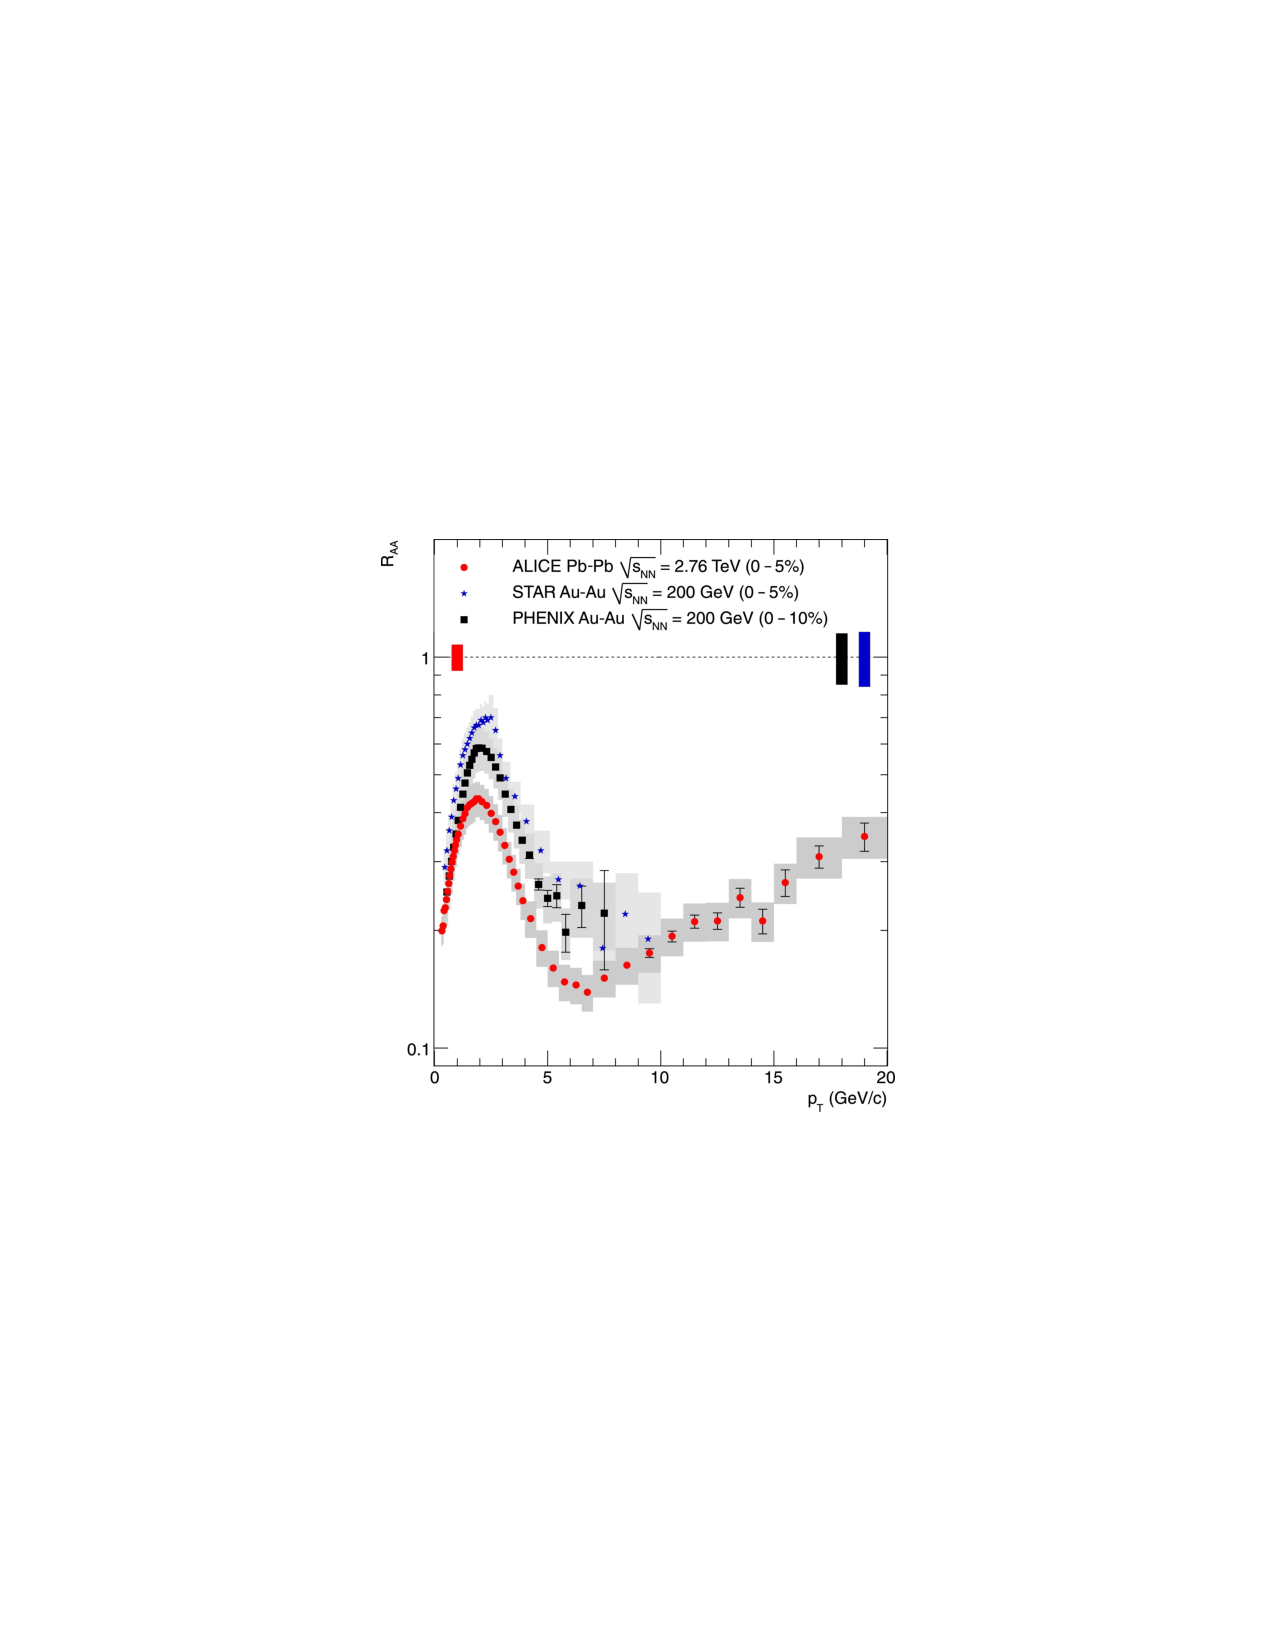
\includegraphics[width=0.7\textwidth]{figures/Theory/ChPart_Raa_ALICE_RHIC.pdf}
\caption[Charged particle $R_{AA}$ at 200 GeV and 2.76 TeV]{Measurements of charged particle $R_{AA}$ from the STAR and PHENIX Collaborations at 200 GeV at RHIC, compared to ALICE results from the LHC at 2.76 TeV from Ref.~\cite{Aamodt:2010jd}.}
\label{fig:alice_chpart_raa}
\end{center}
\end{figure}

\begin{figure}[ht!]
\begin{center}
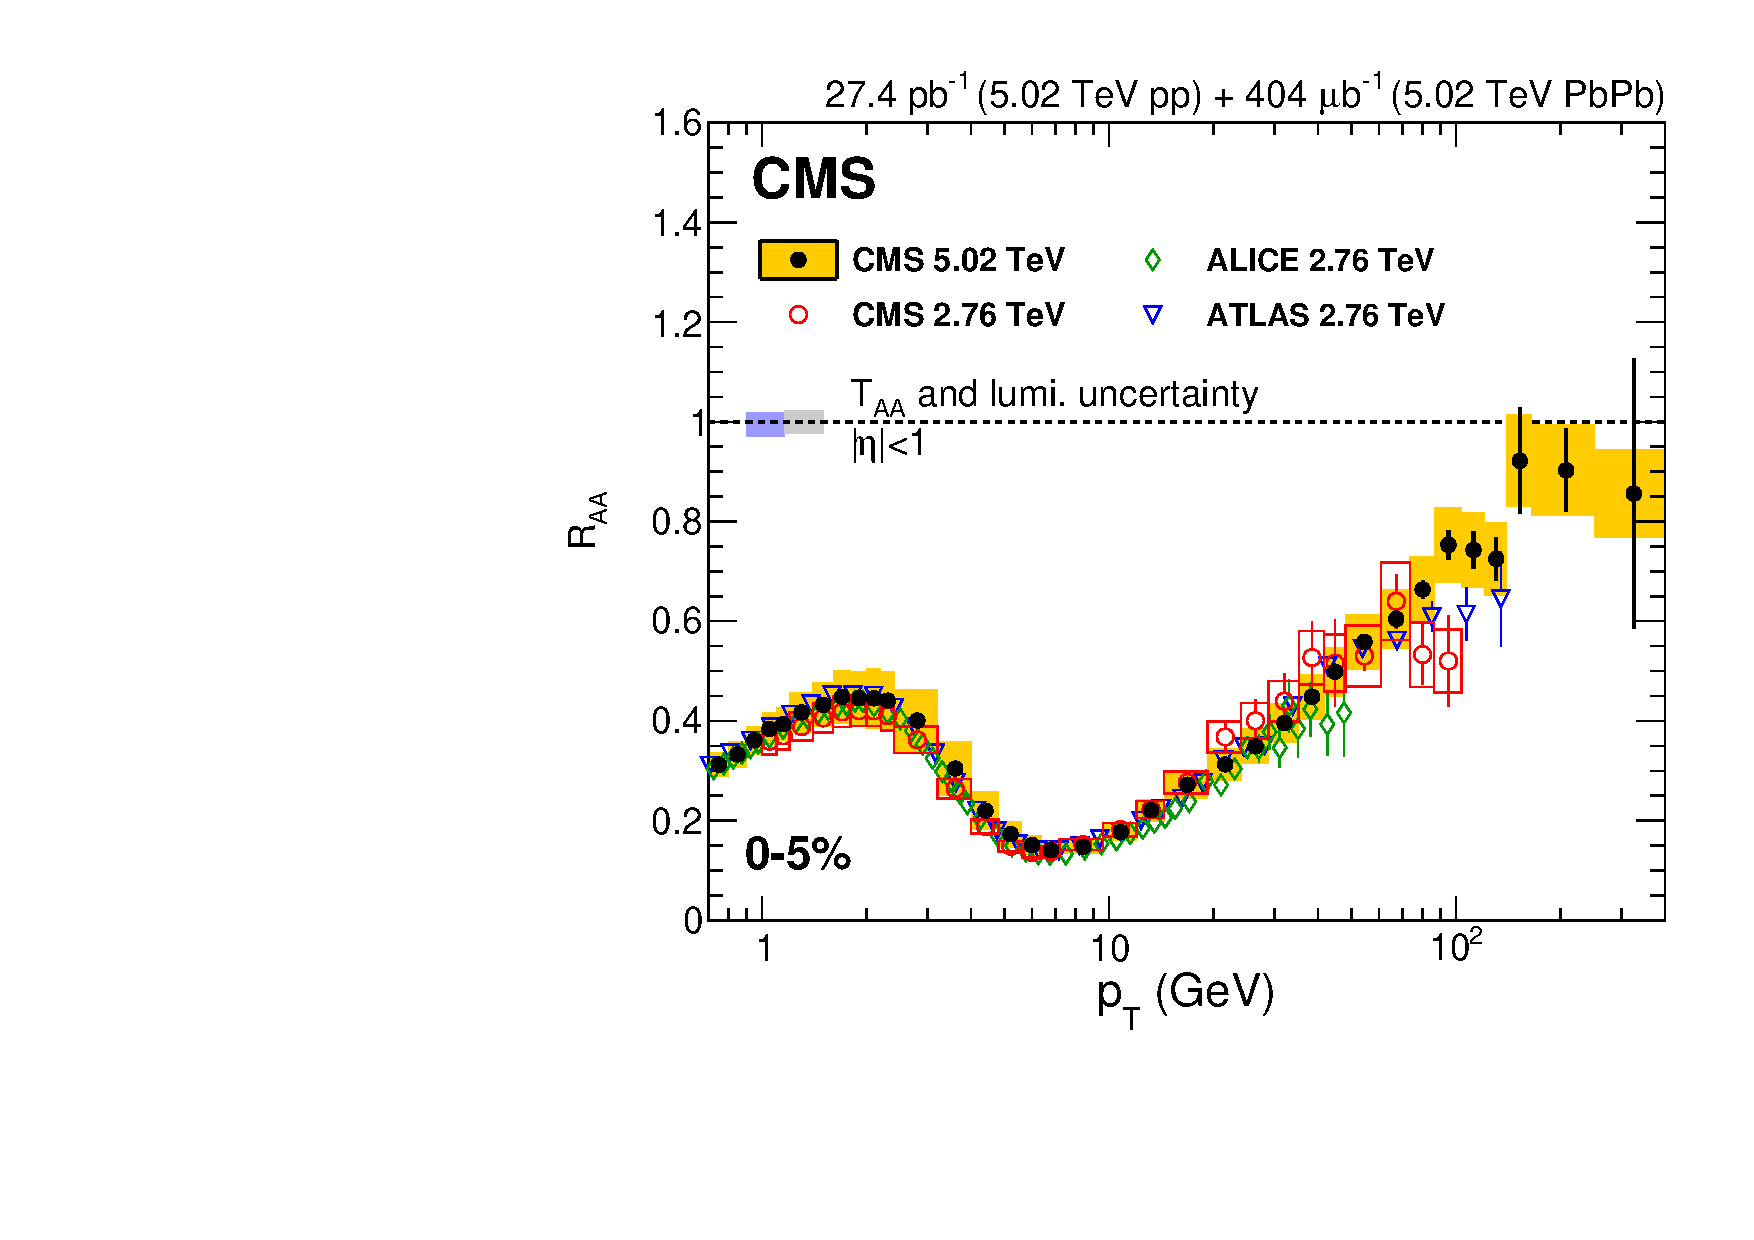
\includegraphics[width=0.7\textwidth]{figures/Theory/ChPart_Raa_CMS_LHC.pdf}
\caption[Charged particle $R_{AA}$ at 2.76 and 5.02 TeV]{Measurements of charged particle $R_{AA}$ at LHC energies 2.76 TeV and 5.02 TeV from Ref.~\cite{Khachatryan:2016odn}.}
\label{fig:cms_chpart_raa}
\end{center}
\end{figure}


Studies of high-$p_{\rm T}$ tracks make use of the fact that such tracks are likely to originate from outgoing partons in hard-scattering interactions, providing an indirect look at energy loss by the parton used as a probe of the QGP.  To more directly reconstruct parton energy, we may instead consider reconstructed jets, defined as the collection of (spatially grouped) particles resulting from the fragmentation of a high-$p{\rm T}$ quark or gluon.  Jet reconstruction, described in detail in Sec.~\ref{sec:Jets}, groups detector deposits to reconstruct a jet energy, and uses Monte Carlo simulation to reconstruct a ``true'' jet energy of the original parton. 

***** DIAGRAM OF WHAT IS A JET *****

Quenching studies with reconstructed jets therefore can offer a more direct look at energy loss in the medium by comparing measured energy in jets in heavy ion collisions to those in proton-proton collisions.  Measurements of jet $R_{AA}$ at the LHC reported in Refs.~\cite{Aad:2014bxa, Khachatryan:2016jfl} show suppression by a factor of approximately 40-60\% in most central PbPb collisions, with weak depenence on jet $p_{\rm T}$ as shown in Fig.~\ref{fig:cms_jet_raa}.  

\begin{figure}[h!]
\begin{center}
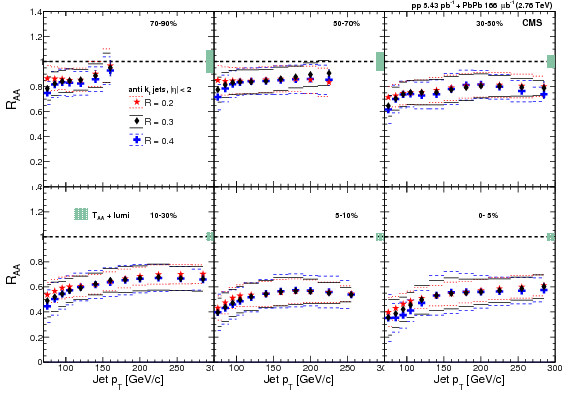
\includegraphics[width=0.99\textwidth]{figures/Theory/JetRaa_CMS.png}
\caption[Jet $R_{AA}$ at 2.76 TeV]{Jet $R_{AA}$ at 2.76 TeV from Ref.~\cite{Khachatryan:2016jfl}.}
\label{fig:cms_jet_raa}
\end{center}
\end{figure}


Jet $R_{AA}$ measurements capture parton energy loss by measuring the reduction in yields in the presence of the QGP.  To connect jet $R_{AA}$ to charged particle $R_{AA}$ measurements, it is necessary to also consider trends in jet fragmentation patterns with jet-$p_{\rm T}$.  High-$p_{\rm T}$ jets are more likely to originate from quarks than from gluons, and therefore exhibit ``harder'' fragmentation patterns--i.e. higher-$p_{\rm T}$ jets fragment into relatively fewer particles each with more $p_{\rm T}$ compared to jets at lower-$p_{\rm T}$.  Jets with softer fragmentation are also expected to exhibit greater modification in the QGP, as low-$p_{\rm T}$ fragmentation products rescatter in the medium.  The highest-$p_{\rm T}$ tracks, for which $R_{AA}$ is the smallest, are associated with those jets that have not only the highest-$p_{\rm T}$, but also the hardest fragmentation.  The high-$p_{\rm T}$ sector of jet $R_{AA}$ measurements at LHC energies, however, still includes significant contributions from jets reconstructed from softer particles that exhibit significant suppression.

\clearpage

\subsection{Jet fragmentation function and jet shape measurements}
\label{sec:jff_jetshapes}

Measurements of jet $R_{AA}$ quantify the overall reduction in numbers of high-$p_{\rm T}$ jets passing a certain momentum threshold, providing an indication of the magnitude of jet energy loss in different $p_{\rm T}$ regions.  As discussed above, this measurement can constrain the possible mechanisms of jet energy loss.  To further constrain models of jet energy loss, additional observables aim to capture the details of jet fragmentation and its modification in the quark gluon plasma.  One such measurement is the jet fragmentation function, which captures the $p_{\rm T}$ distribution of tracks carying jet momentum, paramaterized via the variables $z$ and $\zeta$: 

\begin{equation}
\label{eq:jff_cms}
z = \frac{p^{\rm track}_{\rm ||}}{p^{\rm jet}_{\rm ||}}, \zeta = \frac{1}{{\rm ln} (z)},
\end{equation}

\noindent where $p^{\rm track}_{\rm ||}$ refers to the component of the track $p_{\rm T}$ along the jet axis.  Jet fragmentation function measurements from CMS shown in Fig.~\ref{fig:cms_jff} show a centrality-dependent modification to fragmentation function in PbPb relative to pp data, with a depletion in the mid-$\zeta$ range, balanced by an enhancement at large $\zeta$, in the region corresponding to low-$p_{\rm T}$ tracks.  This shows a redistribution of energy within the jet cone toward softer particle production in the presence of the medium, consistent with predictions of parton energy loss corresponding to a suppression of high-$p_{\rm T}$ particles (model details will be discussed in Sec.~\ref{sec:theory_models}).

\begin{figure}[h!]
\begin{center}
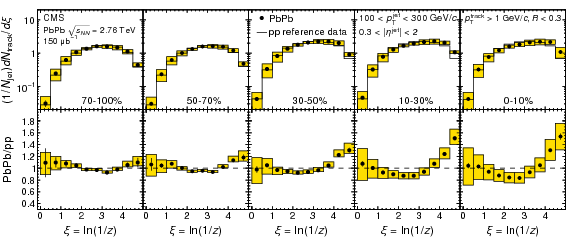
\includegraphics[width=0.99\textwidth]{figures/Theory/CMS_JFF.png}
\caption[Jet fragmentation function in 2.76 TeV PbPb and pp data]{Jet fragmentation function for jets with $100 < p_{\rm T} < 300$ GeV in 2.76 TeV PbPb and pp data from Ref.~\cite{CMS:2012vba}.}
\label{fig:cms_jff}
\end{center}
\end{figure}

In addition to characterizing the $p_{\rm T}$ spectrum of jet constituents, the distribution of $p_{\rm T}$ with respect to the jet axis can also help to constrain fragmentation scenarios.  This distribution, known as the jet shape, is defined within the jet cone as: 

\begin{equation}
\label{eq:jet_shape_cms}
\rho(\Delta r) = \frac{1}{\delta r}\frac{1}{N^{\rm jet}} \mathlarger{ \sum \limits_{\rm jets}} \frac{\Sigma_{{\rm tracks}\in[r_{a},r_{b})} p_{\rm T}^{\rm track}}{p_{\rm T}^{\rm jet}},
\end{equation}

\noindent where $r_{a}$ and $r_{b}$ correspond to the inner and outer radii, respectively, of an annulus of width $\delta r = 0.5$ around the jet axis.  The first jet shape measurement from CMS, shown in Fig.~\ref{fig:cms_jet_shape} (measured with particles with $p_{\rm T} > 1$ GeV), shows a spatial redistribution of energy from small radii ($\Delta r \approx 0.1$) to larger radii ($\Delta r > 0.2$) from the jet axis.  This is qualitatively consistent with predictions of energy redistribution into particles that are both relatively soft ($p_{\rm T} < 3 $ GeV, as observed in jet fragmentation function measurements), and recovered at relatively large angles from the jet axis.  In this way, the study of jet shape modifications $within$ the jet cone motivate extension of these measurements to larger angles from the jet axis to quantify the distribution and $p_{\rm T}$ composition of particles at angles larger than $\Delta r = 0.3$.  

\begin{figure}[hbtp]
\begin{center}
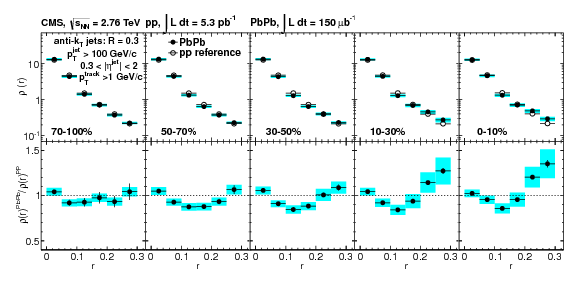
\includegraphics[width=0.99\textwidth]{figures/Theory/CMS_JetShapes.png}
\caption[Jet shape measurement in 2.76 TeV PbPb and pp data]{Jet shape measurement in 2.76 TeV PbPb and pp data from Ref.~\cite{Chatrchyan:2013kwa}.}
\label{fig:cms_jet_shape}
\end{center}
\end{figure}


\clearpage 

\subsection{Dijet asymmetry and momentum balance studies}
\label{sec:dijet_balance}

Additional possibilities for exploration of medium properties follow from the consideration of ``dijets,'' jets that are back-to-back in azimuthal angle ($\Delta \phi_{\rm jets} \approx \pi$).  As the incoming collision participants each begin with $p_{\rm T} \approx 0$ GeV, the total $p_{\rm T}$ of outgoing partons immediately after the collision must also be 0.  If both partons experience either no energy loss (as in the vacuum) or approximately equal energy loss (i.e. by experiencing roughly equal path-lengths through the medium), the measured $p_{\rm T}$ of each jet in the dijet pair would be approximately equal.  If, however, the hard-scattering occurs toward the surface of the QGP, the jet with a longer path-length through the medium might be expected to experience substantially more energy loss, leading to a $p_{\rm T}$ asymmetry in the dijet pair.  This expectation was probed via studies of di-hadron correlations with high-$p_{\rm T}$ particle triggers ($4 < p_{\rm T} < 6$ GeV by STAR at RHIC, $8 < p_{\rm T} < 15 $ GeV by ALICE at the LHC) showed results consistent with the expectation.  These studies showed the substantial suppression (even disappearance, in the STAR studies) of yields of particles with $p_{\rm T} > 2$ GeV in the region opposite the trigger hadron in azimuth~\cite{Adler:2002tq, Aamodt:2011vg}, consistent with path-length dependent jet quenching and a surface bias in trigger particles.  

***** DIAGRAM OF UNBALANCED DIJETS *****

The large kinematic reach of hard probes at the LHC allows for dijet studies at much higher $p_{\rm T}$.  The first of these studies measured the ``dijet imbalance'' between the highest-$p_{\rm T}$ (``leading jet,'' with $p_{\rm T,1}$) and second-highest-$p_{\rm T}$ jets (``subleading jet,'' with $p_{\rm T, 2}$ in the event, parameterized as: 

\begin{equation}
\label{eq:aj}
A_{\rm J} = \frac{p_{\rm T,1} - p_{\rm T,2}}{p_{\rm T,1} + p_{\rm T,2}}
\end{equation}

\noindent These studies, by the ATLAS and CMS Collaborations~\cite{Aad:2010bu, Chatrchyan:2011sx} showed a centrality-dependent shift in the $A_{\rm J}$ in PbPb collisions, with greater dijet asymmetry in central PbPb data than in pp or in peripheral PbPb collisions.  In pp and peripheral PbPb collisions, asymmetric dijet events are those in which some $p_{\rm T}$ is carried by a third jet, and the $A_{\rm J}$ distribution is steeply falling.  In central PbPb collisions, however, there are expected to be two contributions to the sameple of asymmetric dijet events: not only three-jet events, but also dijet events in which the subleading jet is substantially quenched.  As shown Fig.~\ref{fig:cms_dijets}, this effect is evident in the shift toward larger values of $A_{\rm J}$ in central PbPb collisions. 

\begin{figure}[hbtp]
\begin{center}
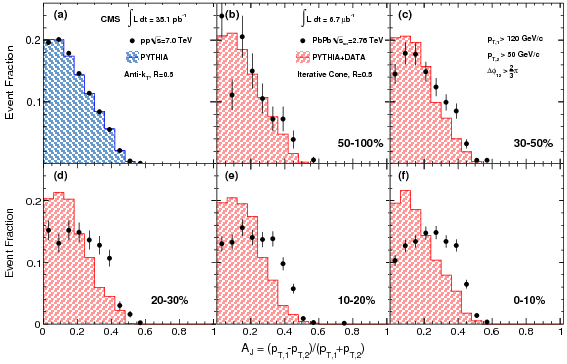
\includegraphics[width=0.9\textwidth]{figures/Theory/CMS_dijets.png}
\caption[Dijet asymmetry and in 2.76 TeV PbPb and pp data]{Dijet asymmetry in 2.76 TeV PbPb and pp data for jet selection $p_{\rm T,1} > 120$ GeV, $p_{\rm T,2} > 50$ GeV, and $\Delta\phi_{\rm 1,2} > 2\pi/3$ from Ref.~\cite{Chatrchyan:2011sx}.}
\label{fig:cms_dijets}
\end{center}
\end{figure}

The transverse momentum difference between the leading and subleading jets may be conceptualized as ``missing-$p_{\rm T}$'' from the subleading jet, which must by momentum conservation be recovered somewhere in the hemisphere of the event surrounding the subleading jet axis.  One way to capture this momentum balance is by comparing the total $p_{\rm T}$ carried by tracks in different $p_{\rm T}$ classes in the subleading relative to the leading hemisphere.  This balance is shown in the top row Fig.~\ref{fig:cms_mpT}, for $\slashed{p}_{\rm T}^{\rm ||}$ defined as the projection of each track's $p_{\rm T}$ projected in $\phi$ onto the dijet axis (i.e. the average of the leading and subleading jet axes)~\ref{HIN_2014_010}.  In pp and peripheral PbPb data, this balance shows the depletion of tracks with $p_{\rm T} > 8$ GeV in the subleading relative to the leading hemisphere balanced primarily by tracks with $2 < p_{\rm T} < 8$ GeV, consistent with the localization of these tracks in additional jets for unbalanced dijets in this scenario.  The magnitude of the ``missing-$p_{\rm T}$'' balancing distribution increases with growing $A_{\rm J}$ by construction.  Comparing PbPb to pp distributions (differences shown int he bottom row of Fig.~\ref{fig:cms_mpT}), the balancing distribution in unbalanced (large $A_{\rm J}$) events in central PbPb data shows larger contributions from soft particles with $p_{\rm T} < 2$ GeV and smaller contributions from particles with $p_{\rm T} > 4$ GeV, indicating that the more of the balancing $p_{\rm T}$ distribution in the subleading side is carried by soft quenching products rather than additional jets. 


\begin{figure}[hbtp]
\begin{center}
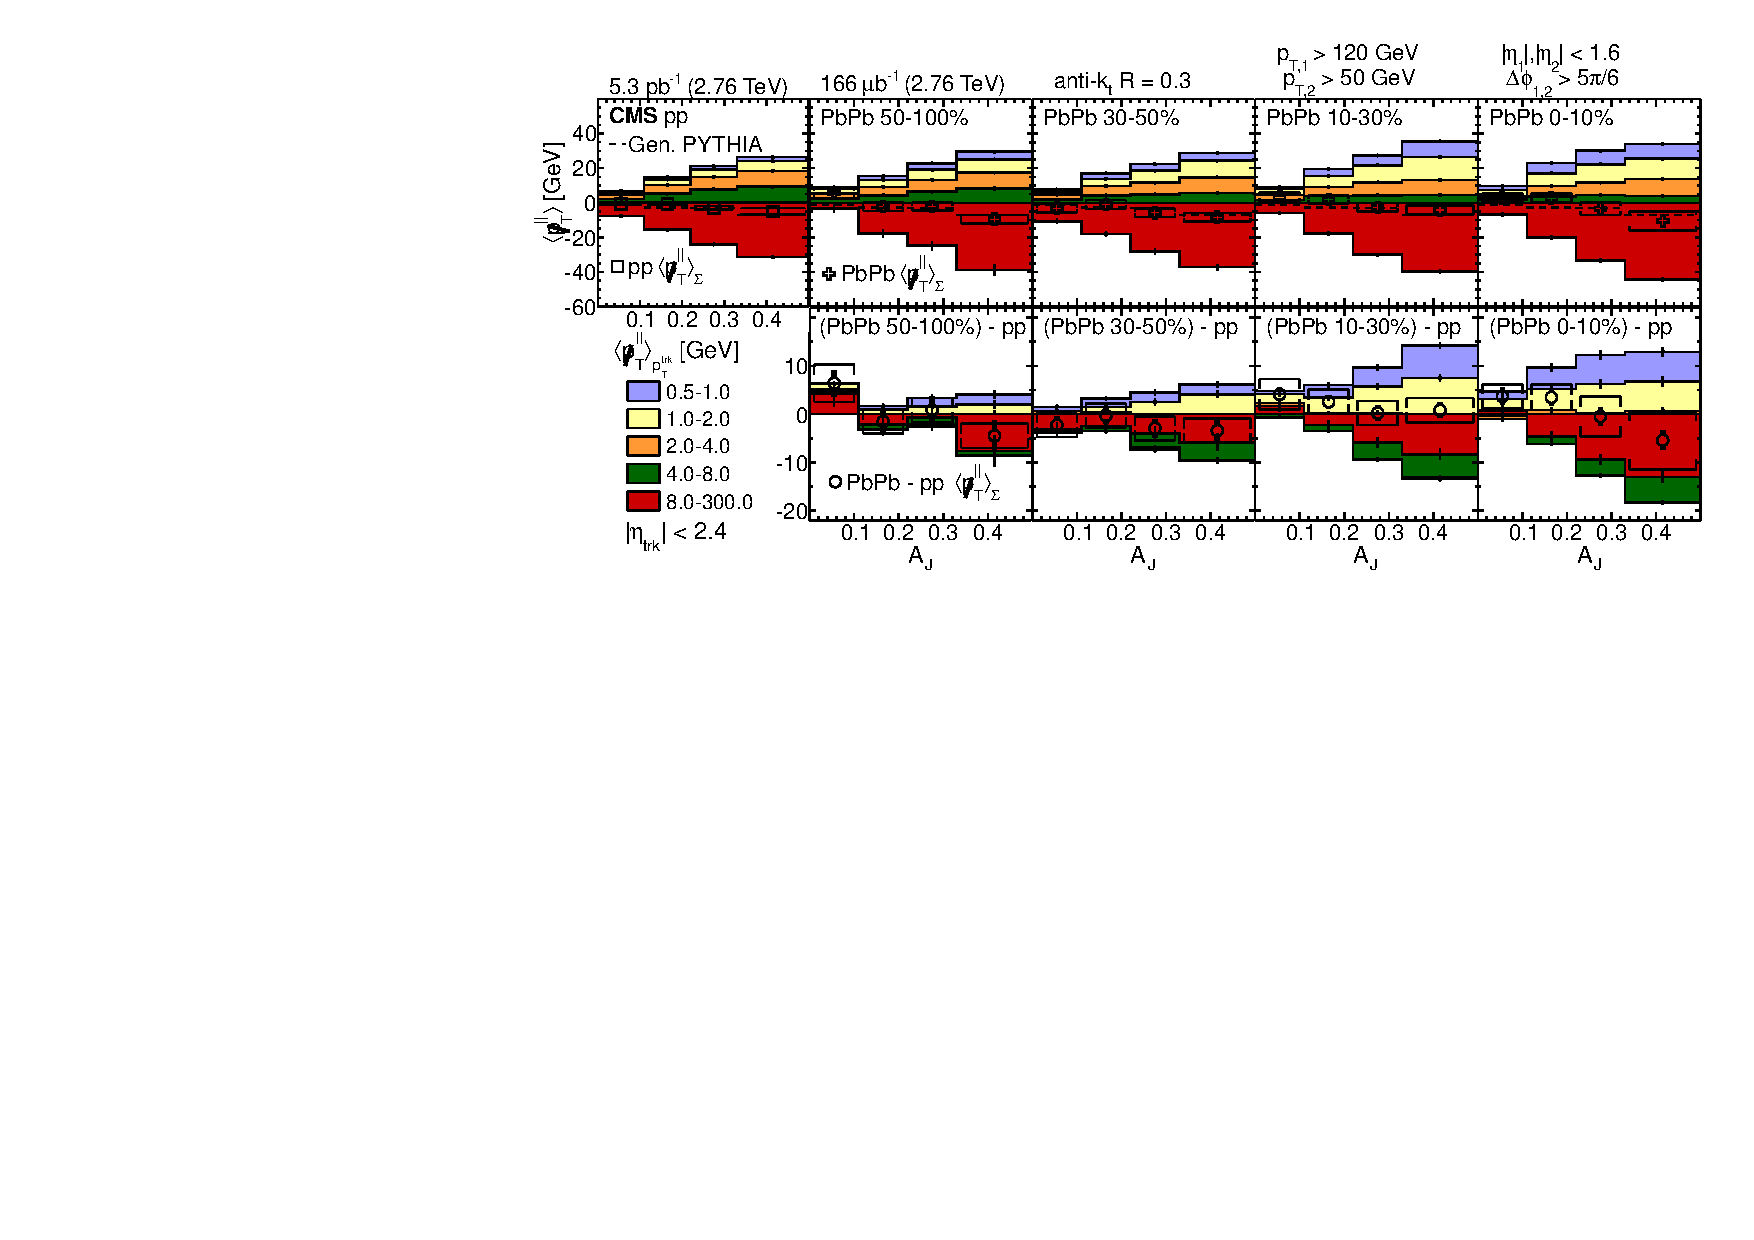
\includegraphics[width=0.99\textwidth]{figures/Theory/CMS_mpT.pdf}
\caption[Hemisphere $p_{\rm T}$ momentum balance in dijet events as a function of $A_{\rm J}$]{Top row: hemisphere $p_{\rm T}$ momentum balance in dijet events as a function of $A_{\rm J}$, taking the total difference $\slashed{p}_{\rm T}^{\rm ||}$ in the subleading hemisphere minus that in the leading hemisphere from Ref.~\ref{HIN_2014_010} in pp and PbPb data.  Bottom row:  Differences PbPb - pp.}
\label{fig:cms_mpT}
\end{center}
\end{figure}

Dijet momentum balance studies therefore show evidence of redistribution of jet energy from harder to softer particles via jet quenching, and greater quenching of the subleading than leading jets.  As discussed above, the angular distribution of quenching products relative to the jet axis is also highly relevant for constraining models of interactions between the jet and the medium.  This measurement is shown in Fig.~\ref{fig:cms_mpT_unbalanced} for unbalanced dijets with $A_{\rm J} > 0.22$.  Comparing the radial distribution with respect to the dijet axis shows that in this unbalanced dijet sample in central PbPb events, more $p_{\rm T}$ is recovered in lower-$p_{\rm T}$ particles extending to large angles from the jet axis.  It is important to note that this measurement shows overall hemisphere differences in the radial $p_{\rm T}$ distribution, combining the effects of quenching to the subleading jet, quenching to the leading jet, and also any azimuthal asymmetry in the underlying event (as would arise if the direction of the dijet axis coupled to odd underlying event flow terms such as $v_{\rm 3}$).  Isolating and further studying each of these contributions will be a major goal of this analysis, as discussed in Sec.~\ref{sec:motivation_decomp}.


\begin{figure}[hbtp]
\begin{center}
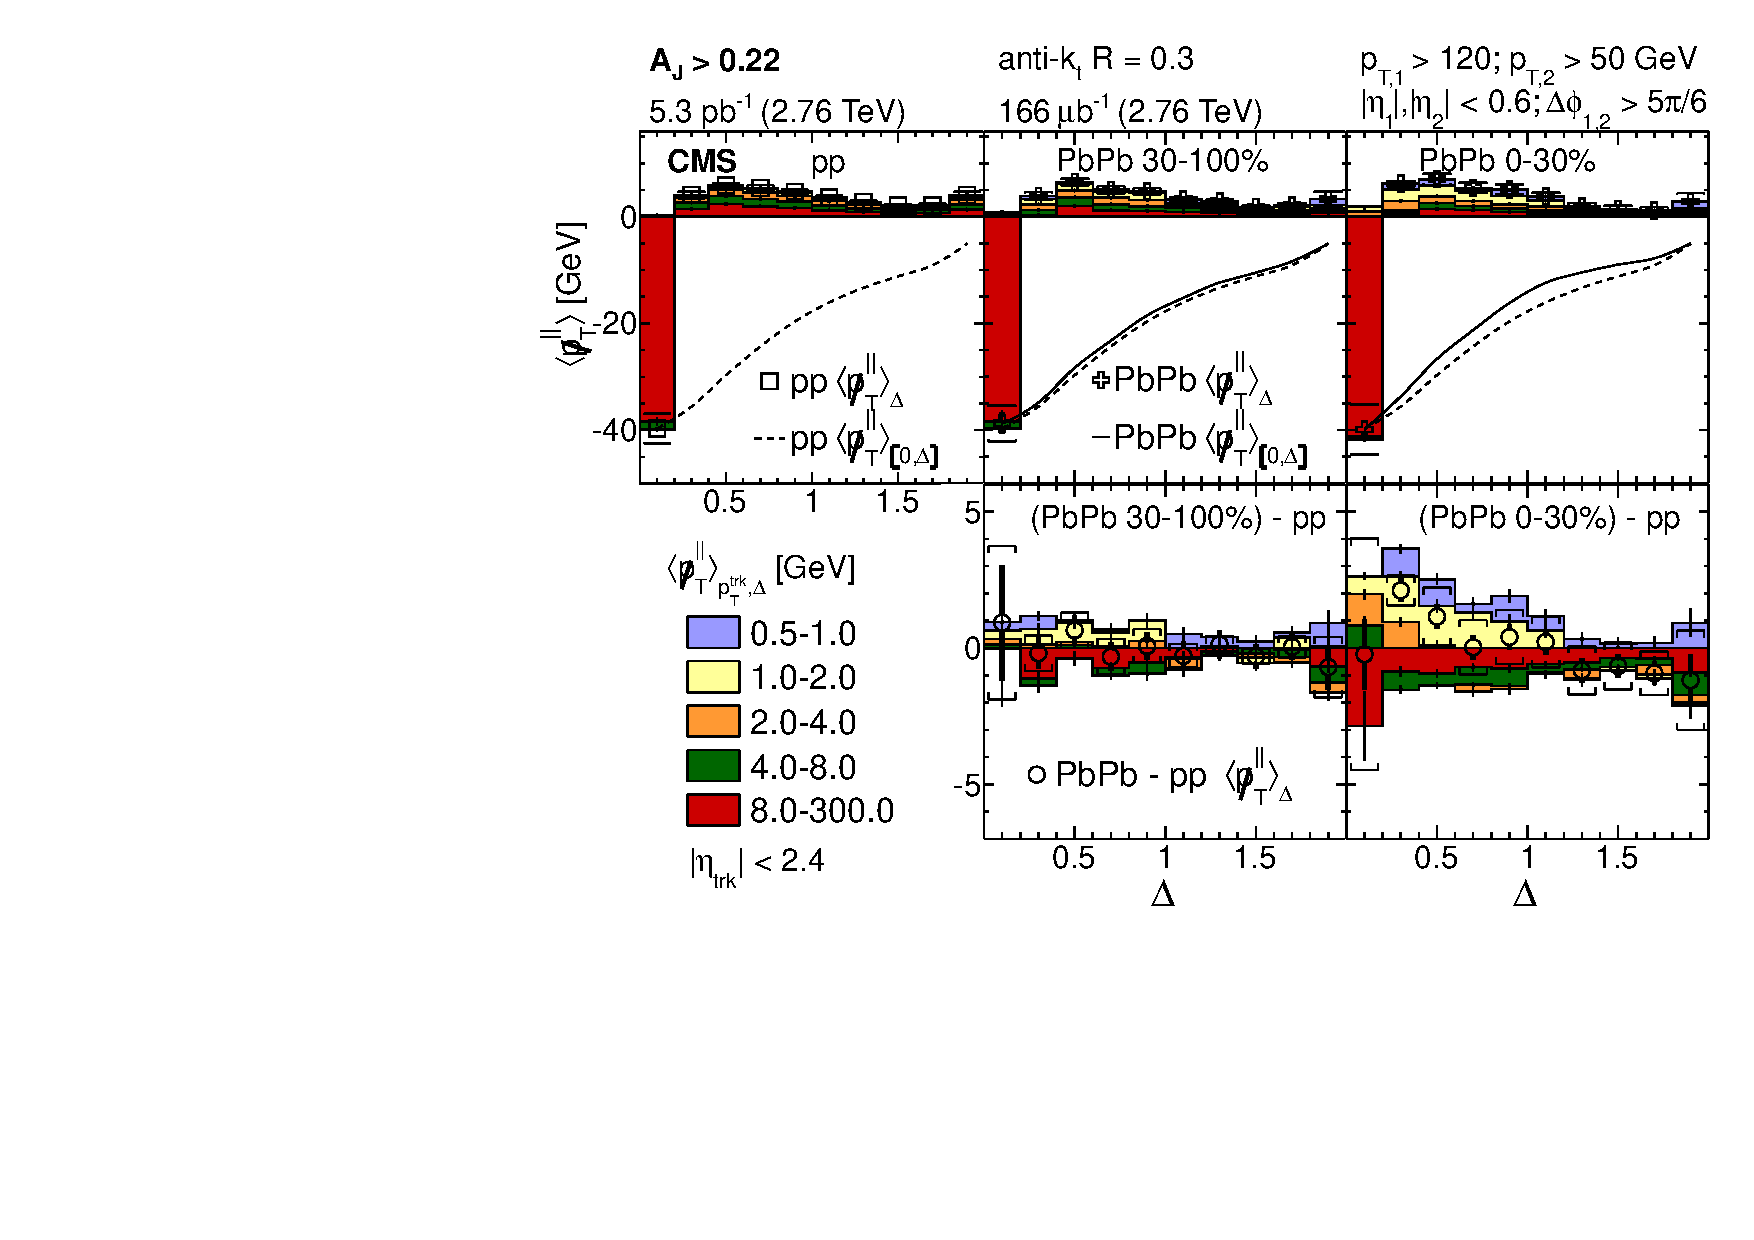
\includegraphics[width=0.9\textwidth]{figures/Theory/MpT_Unbalanced.pdf}
\caption[]{}
\label{fig:cms_mpT_unbalanced}
\end{center}
\end{figure}




\clearpage


\section{Models of jet energy loss in the quark gluon plasma}
\label{sec:theory_models}

A range of theoretical models of jet quenching have been developed to specifically account for the energy loss of a propagating probe through the quark gluon plasma.  In general, models characterize collisional energy loss mechanisms (i.e. jet energy loss via elastic interactions with the medium), radiative energy loss by the propagating parton, and in some cases a medium response in the form of a ``plasma wave'' or back reaction.  Some prominent examples of specific quenching models are surveyed briefly in Sec.~\ref{sec:model_survey}.  Some relevant comparisons to data are shown in Sec.~\ref{sec:model_comparison}, and then Sec.~\ref{sec:motivation} summarizes goals of the present analysis in the context of the current state of jet quenching models. 

\subsection{Survey of theoretical models of jet quenching mechanisms}
\label{sec:model_survey}

pQCD works down to 1 GeV...

\begin{itemize}

\item DGLV (and CUJET implementation)
\item BDMPS-Z/ASW (and JEWEL implementation)
\item Higher-Twist
\item AMY (McGill and MARTINI implementations)
\item Soft collinear effective theory with glauber gluons
arxiv:1509.07257
https://arxiv.org/pdf/1601.04695.pdf

\item Linear Boltzman Transport model
https://arxiv.org/pdf/1703.00822.pdf

\item Strong/weak hybrid model from AdS/CFT
arXiv:1101.0618v2
arXiv:1609.05842

\item Coupled jet-fluid model
 arXiv:1701.07951


\end{itemize}

Nice summary of these
https://arxiv.org/pdf/1312.5003.pdf

\subsection{Quenching model comparisons to high-$p_{\rm T}$ particle and jet observables}
\label{sec:model_comparison}

\subsubsection{Quenching model comparisons: $R_{AA}$}

\begin{figure}[hbtp]
\begin{center}
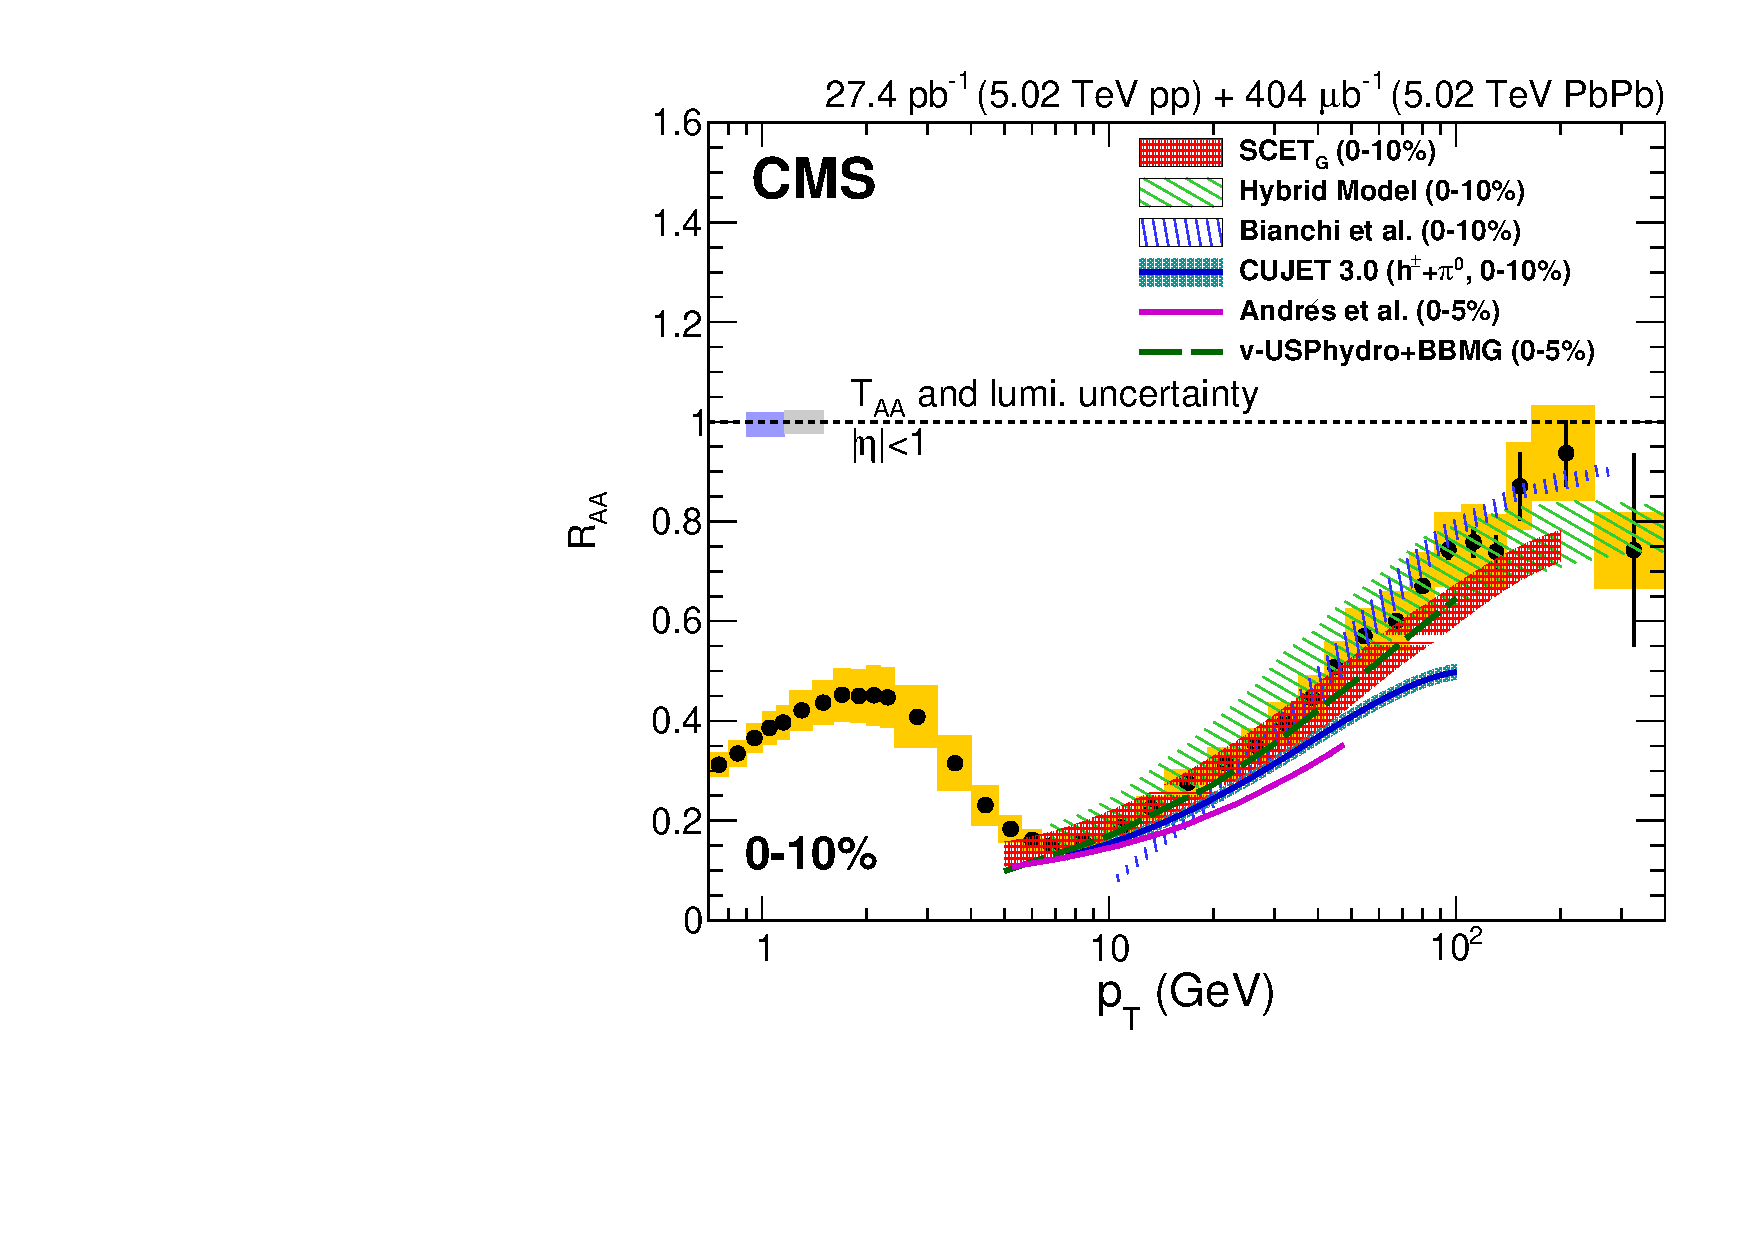
\includegraphics[width=0.7\textwidth]{figures/Theory/ChPart_Raa_CMS_Theory.pdf}
\caption[Model comparisons to charged particle $R_{AA}$ at 5.02 TeV]{Model comparisons to charged particle $R_{AA}$ in 0-10\% central PbPb data at 5.02 TeV from Ref.~\cite{Khachatryan:2016odn}.}
\label{fig:cms_chpart_raa_theory}
\end{center}
\end{figure}



\subsubsection{Quenching model comparisons: jet fragmentation functions}

\subsubsection{Quenching model comparisons: jet shapes}

\subsubsection{Quenching model comparisons: dijet asymmetry}
  
  
  
 \subsection{Theoretical motivations for detailed jet-track correlation studies}
 \label{sec:motivation}
 
  \subsubsection{Extenshion of jet shape measurements to large angles}
  
  \subsubsection{Detailed characterization of jet peak in separate dimensions $\Delta\eta$ and $\Delta\phi$}
  
  \subsubsection{Detailed characterization of leading and subleading jet peaks in dijet events}
  
  \subsubsection{Decomposition of contributions to momentum balance studies in dijet events}
  \label{sec:motivation_decomp}
  
  
\clearpage

\section{The Large Hadron Collider and the CMS detector}
\label{sec:Detector}

\subsection{The Large Hadron Collider}

The Large Hadron Collider (LHC), located at CERN near Geneva, is the largest and highest-energy particle accelerator in the world.  It consists of two counter-rotating particle beam line in a tunnel 26.7 km in circumference, located between 45 m and 170 m underground~\cite{Evans:2008zzb}.  During standard operation, the LHC collides beams of protons accelerated and focused using a series of superconducting magnets, cooled to below 2 K using supercritical helium.  Particle beams are brought together for collisions at in experimental detectors at four points in the accelerator ring:  the ATLAS, CMS, ALICE, and LHCb detectors.  In addition to the proton-proton (pp) data collected at center-of-mass energies $\sqrt{\rm S_{NN}} = 7$ TeV, 8 TeV, and 13 TeV, the LHC has also been operated for heavy ion physics by colliding with fully-stripped lead nuclei ($\rm ^{182}Pb^{82+}$) in lead-lead (PbPb) and proton-lead (pPb) collisions.  Heavy ion runs at the LHC have included PbPb data and pp ``reference'' runs at $\sqrt{\rm S_{NN}} = 2.76$ TeV (2011 and 2013, respectively) and 5.02 TeV (2015) and pPb data at $\sqrt{\rm S_{NN}} = 5.02$ TeV (2013 and 2016) and 8.16 TeV (2016).  This analysis relies on PbPb data at 2.76 TeV and 5.02 TeV, and corresponding pp reference data at the same center-of-mass energies. 

In peak proton-proton operation, the LHC collides 2,808 bunches each containing approximately $10^{11}$ protons with a minimum bunch spacing of 25 ns, for a maximum luminosity of $10^{34}\rm cm^{-2}s^{-1}$ delivered to the high-luminosity detectors (ATLAS and CMS).  The lead-lead performance target of $10^{27}\rm cm^{-2}s^{-1}$ delivered via 592 bunches of $10^{7}$ lead ions was slightly exceeded during the 2015 PbPb run.  At this high-intensity frontier, it is common during nominal pp data collection and possible in PbPb data collection that multiple distinct proton-proton collisions may occur within a recorded event in a phenomenon known as ``pile-up.''  However, pile-up is relatively rare in PbPb collisions due to the lower luminosities, and in the present analysis only one primary vertex will be considered (with products of any other possible interactions removed via background subtraction procedures). 

\subsection{The CMS detector}

The CMS detector is named for the Compact Muon Solenoid at its heart:  a superconducting magnet with magnetic field of 3.8 T, length of 13 m, diameter of 6 m, and weight 14,000 tons.  Inside of this solenoid, the detector includes silicon pixel and strip detectors for particle tracking (see Sec.~\ref{sec:trackers} for a detailed explanation), and electromagnetic and hadronic calorimeters (see Sec.~\ref{sec:calorimeters}).  Calorimeters within the solenoid volume are complemented by additional calorimetry outside of the solenoid that provides coverage in the very forward direction close to the beam line, including the hadronic forward (HF) calorimeter in the region $3.0 < |\eta| < 5.2$ used in this analysis for centrality determination, and the Zero Degree and CASTOR calorimeters in the even more forward region.  The CMS detector also includes an extensive muon system outside of the solenoid volume, consisting of aluminum drift tubes in the barel region, cathode strip chambers in the forward region, and a complementary system of resistive plate chambers (not discussed in detail here as muons are not of primary relevance to this analysis).  Full details about the CMS detector may be found in Ref.~\cite{Chatrchyan:2008zzk}, and a perspective drawing of the CMS detector from this report is shown in Fig.~\ref{fig:detector}.

In the CMS detector, the +z axis is defined to be horizontal, pointing to the West along the beam line direction.  The x axis is horizontal, pointing to the South toward the center of the LHC.  The +y axis is vertical, pointing upward.  The azimuthal angle $\phi = \rm tan^{-1}(\frac{y}{x})$ is defined in the x-y plane such that $\phi = 0$ is the +x axis.  Pseudorapidity $\eta = \rm -ln(tan(\frac{\theta}{2})$ is defined to have the same sign as the +z axis.  Pseudorapidity coverage in the CMS detector ranges from $\eta = 0$ at the y-axis, to $|\eta| > 8.3$ in Zero Degree Calorimeter approaching the +/-z axis.

\begin{figure}[hbtp]
\begin{center}
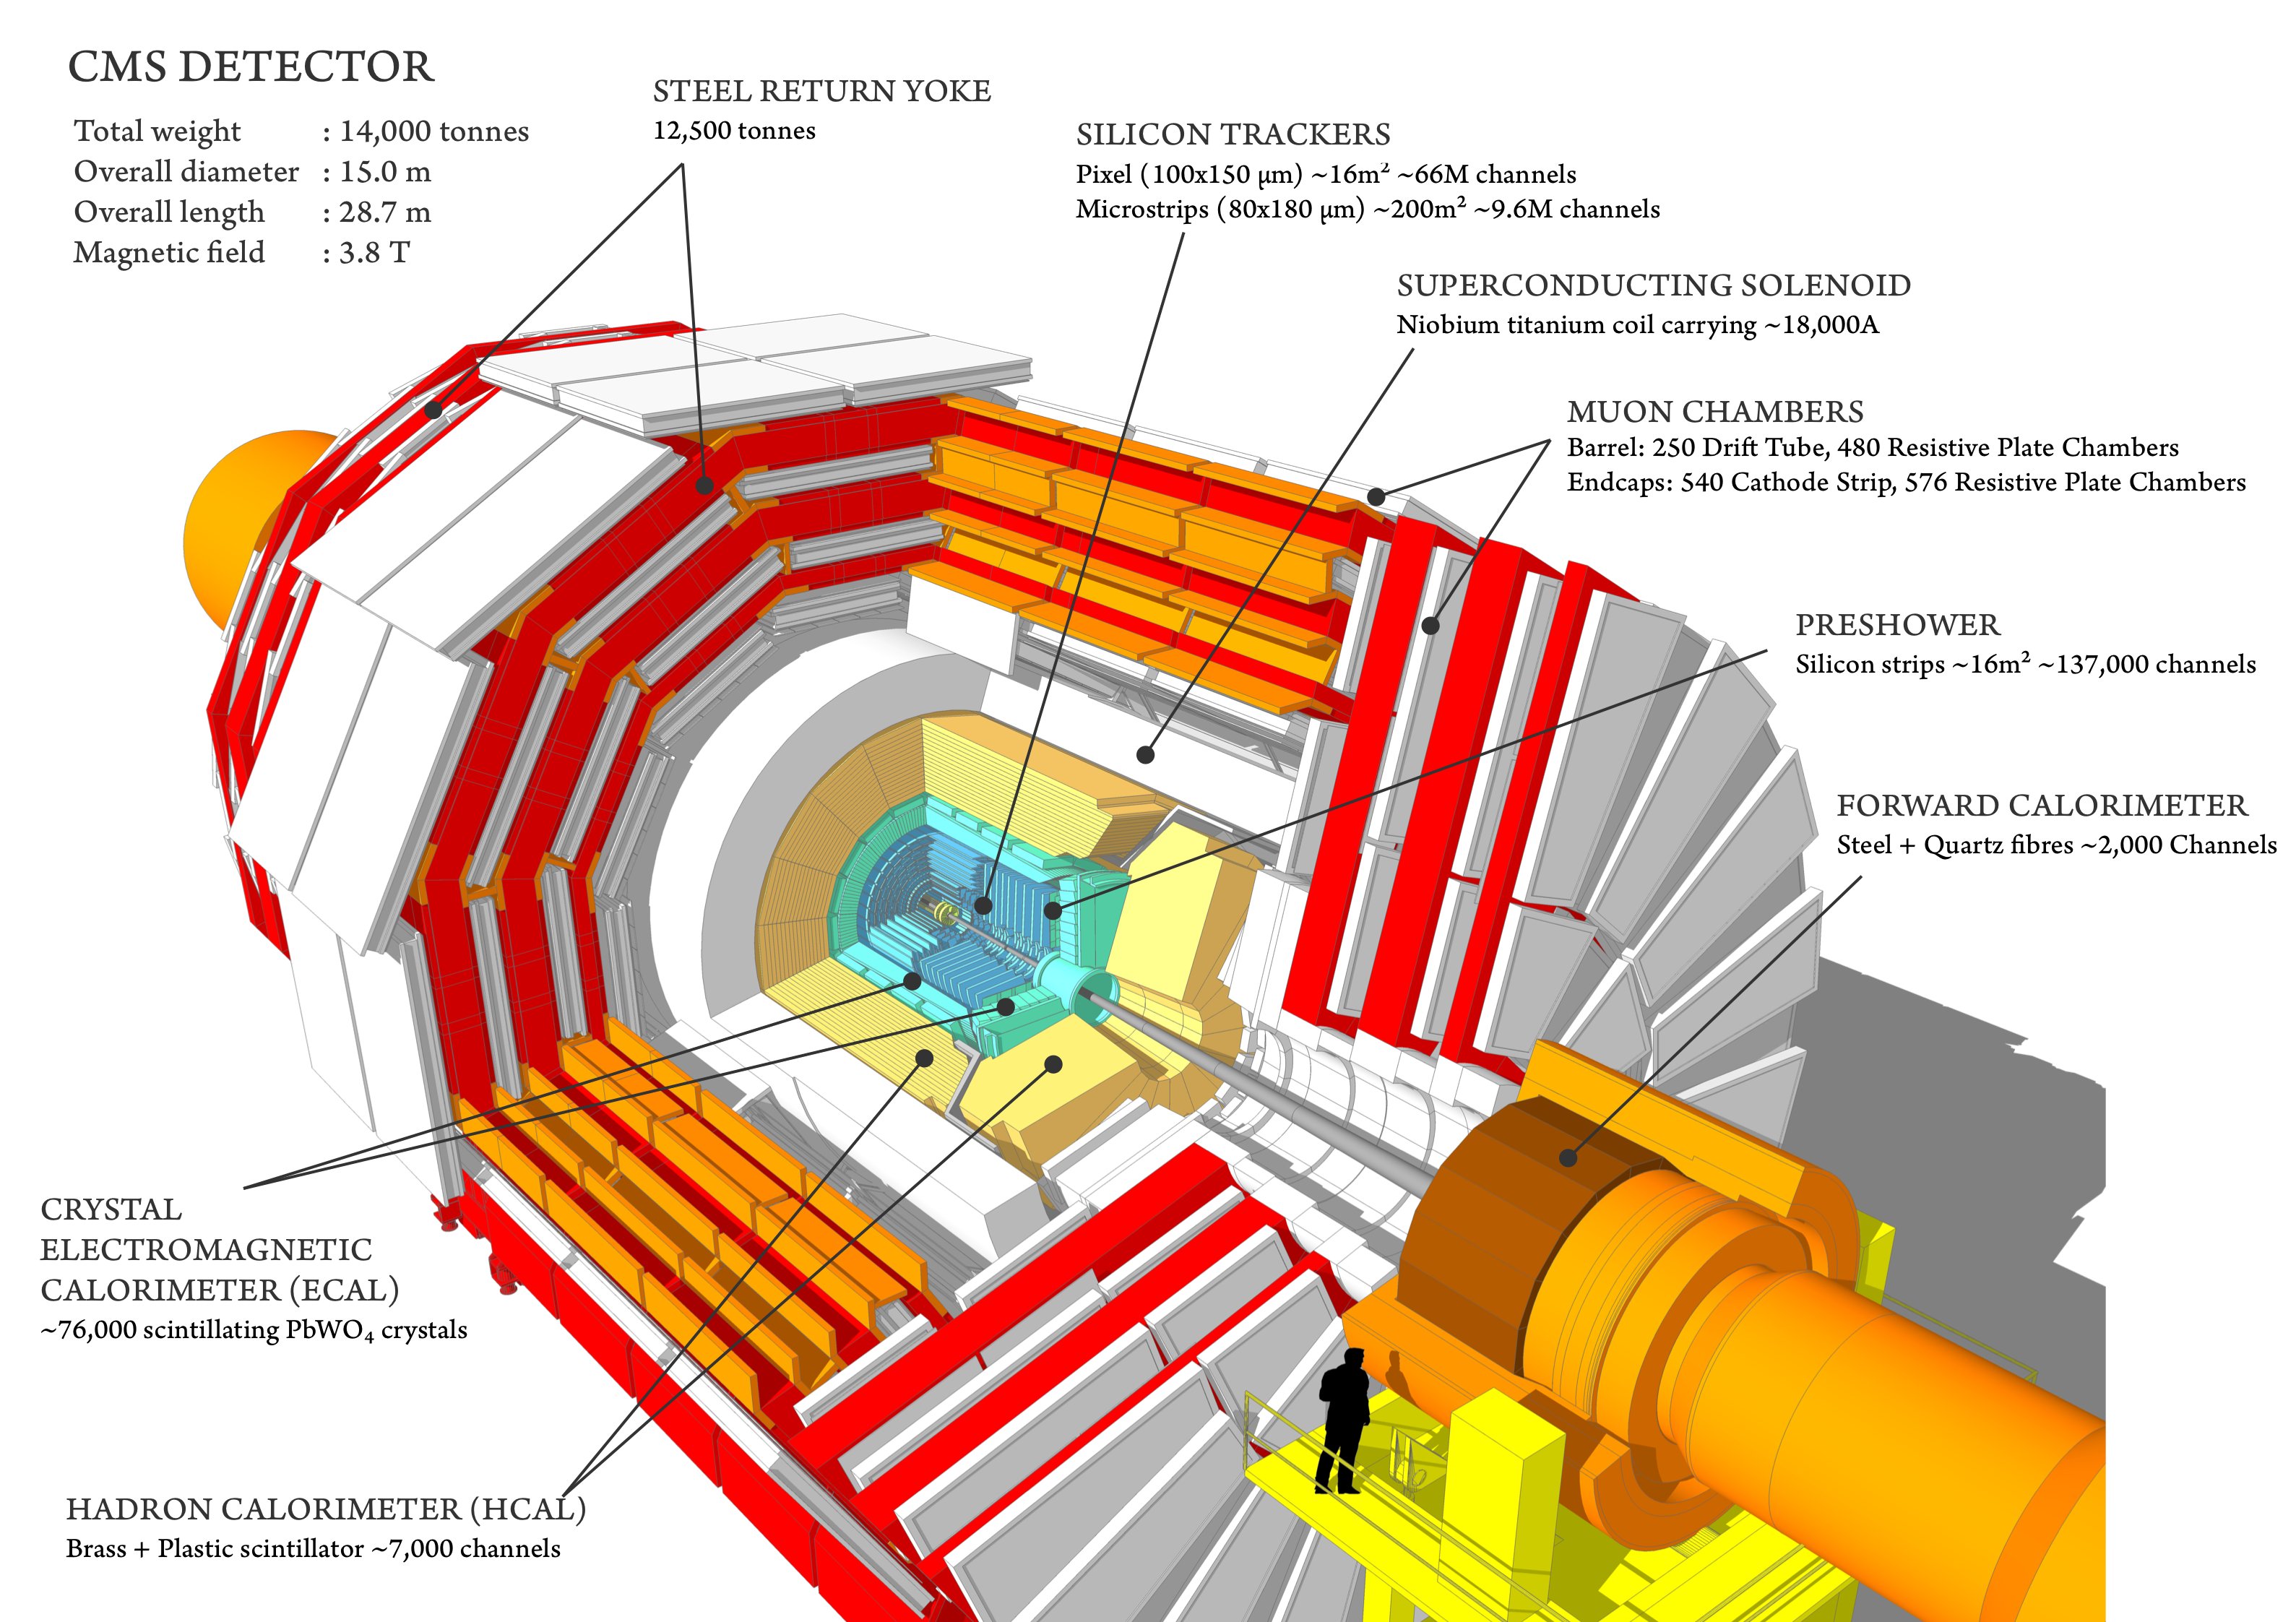
\includegraphics[width=0.9\textwidth]{figures/Detector/Detector.png}
\caption[CMS detector perspective drawing]{Perspective rendering of the CMS detector, showing component sub-detectors with a human included for scale perspective~\cite{SketchUp}.}
\label{fig:detector}
\end{center}
\end{figure}

\subsection{Trackers in the CMS detector}
\label{sec:trackers}

The CMS tracking system consists of a small silicon pixel detector for precise measurement near the interaction point (with three layers with radii 4.4 cm to 10.2 cm), surrounded by a large silicon strip detector with layers to a radius of 110 cm.  In both detectors, a cylindrical tracker ``barrel'' is complemented by ``endcap'' disks that together provide full azimuthal coverage and pseudorapidity coverage in the range $|\eta| < 2.5$.  The pixel detector consists of 66 million pixels in 1440 modules.  It provides three-dimensional measurements of ``hits,'' or interactions of particles with tracker materials, with a transverse resolution $10 \mu$m and longitudinal resolution $20 - 40 \mu$m (and a third coordinate provided by the pixel plane).  The silicon strip detector consists of 9.3 million strips in 15,148 modules, organized in four components:  Tracker Inner Barrel (TIB) and Disks (TID), Tracker Outer Barrel (TOB, covering the region $r > 55 \rm$ cm), and Tracker End Caps (TEC, covering the region $124 < |z| < 282$ cm).  Figure~\ref{fig:tracker} shows a diagram of the pixel and strip detectors, which have total length 5.8 m and diameter 2.5 m~\cite{Chatrchyan:2014fea}.  Track reconstruction and tracking efficiency will be discussed in detail in Sec.~\ref{sec:Tracks}.


\begin{figure}[hbtp]
\begin{center}
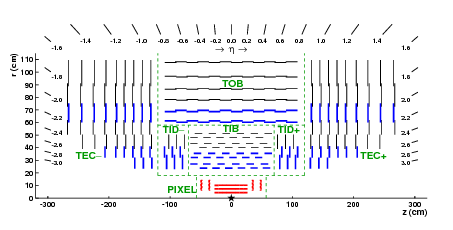
\includegraphics[width=0.7\textwidth]{figures/Detector/figs_2011_cmsTracker_TrackerLayoutNew.png}
\caption[Diagram of CMS trackers]{Diagram of CMS pixel and silicon strip detectors in the $r-z$ plane~\cite{Chatrchyan:2014fea}.}
\label{fig:tracker}
\end{center}
\end{figure}



\subsection{Calorimeters in the CMS detector}
\label{sec:calorimeters}

This analysis relies on electromagnetic and hadronic calorimeters for the energy measurements used as inputs for the reconstruction of high-$p_{\rm T}$ jets.  The ECAL, which measures the energy of charged particles, consists of 75\,848 lead tungstate ($\rm PbWO_{4}$) crystal scintillators, organized in $5 \time 5$ arrays, covering $|\eta| < 1.48 $ in a barrel region and $1.48 < |\eta| < 3.0$ in the endcap region.  Light from the scintillators is captured with avalanche photodiodes in the barrel region, and vacuum phototriodes in the endcap region.  A preshower detector system in front of the ECAL is used to assist in the identification of neutral pions and electrons~\cite{Chatrchyan:2008zzk}.  ECAL energy resolution ranges from about 1-2.5\% (depending $|\eta|$ and photon conversion) in the barrel region, and from 2.5-4\% in the endcap region.~\cite{CMS:EGM-14-001}. 

Hadrons pass through the ECAL and are stopped by the HCAL, a hermetic detector which records their energy using a system of scintellator tiles embedded with wavelength-shifting  fibers.  The HCAL has three regions, as shown in Fig.~\ref{fig:HCAL}:  barrel (HB), endcap (HE), and an outer region (HO) outside of the solenoid, necessitated by the fact that the HB is volume-limited by the solenoid diameter.  In the barrel region $|\eta| < 1.74$, the HCAL cells have widths of 0.087 in pseudorapidity and 0.087 in $\phi$, while for $|\eta| > 1.74$ the coverage of the towers increases progressively to a maximum of 0.174 in $\Delta \eta$ and $\Delta \phi$.  HCAL towers are mapped onto ECAL towers within the barrel region, and their summed energies are used to determine the location, energy, and axis of jets, as described below in Sec.~\ref{sec:Jets}.  The HCAL is complimented in the forward region by the HF calorimeters, which each consist quartz fibers in the $\pm z$ directions organized in 432 readout towers in the region $3.0 < |\eta| < 5.2$~\cite{Chatrchyan:2008zzk}.  In this analysis, only jets from the barrel region of the calorimeters wil be included, while the HF detector is used for the determination of PbPb event centrality as described in Sec.~\ref{sec:centrality}. 

\begin{figure}[h!]
\begin{center}
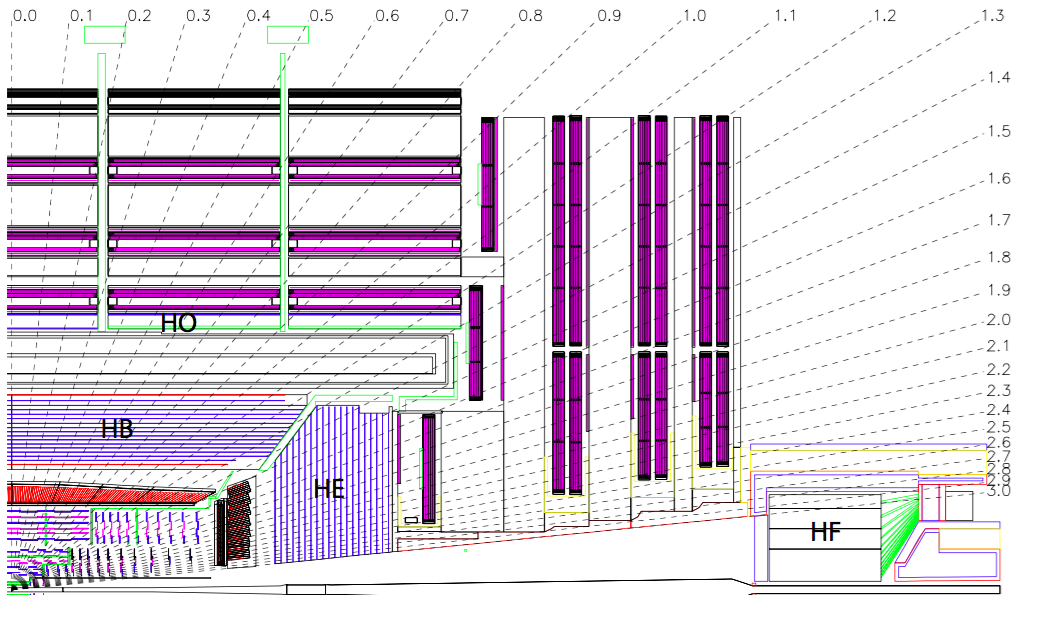
\includegraphics[width=0.6\textwidth]{figures/Detector/HCAL_Diagram.png}
\caption[Diagram of the HCAL]{Diagram of the HCAL~\cite{Chatrchyan:2008zzk}.}
\label{fig:HCAL}
\end{center}
\end{figure}

\subsection{The CMS trigger system}
\label{sec:HLT}

The collision rate at in the LHC is so high that it is impossible to store and process every event that occurs in the CMS detector.  A two-level online trigger system is therefore used to select events of interest.  Furthermore, data selected with loose trigger requirements (for example ``zero bias'' data with no selection criteria and ``minimum bias'' criteria consisting of minimal requirements to demonstrate the presence of a collision event) may also need to be further ``prescaled'' to limit the rate of recorded events by a specified factor.  The trigger system consists of a first (L1) trigger consisting of progammable electronics that use information from the calorimeter and muon systems of the detector to select events to record.  The L1 trigger opperates with an interval of approximately $4 \mu$ s, with a maximum rate of 100 kHz.  The next trigger level, the High Level Trigger (HLT), consists of a processor farm that allows for more sophisticated event selection based on the reconstruction of physics objects.  Reconstruction is performed in a series of steps, or a ``HLT path,'' chosen to apply selection in order of increasing reconstruction complexity, so as to minimize processing time~\cite{Khachatryan:2016bia}.  This analysis will rely primarily on two kinds of triggers:  minimum bias data, and jet-triggered data samples selected by requiring the presence of an online reconstructed jet with $p_{\rm T} > 80 $ GeV ($p_{\rm T} > 100 $ GeV for 5.02 TeV PbPb data).  No prescale is applied for the jet-triggered data samples used in this analysis.  






\clearpage

\section{Track reconstruction and correction}
\label{sec:Tracks}
\subsection{Track reconstruction in pp collisions}

Standard track reconstruction in CMS occurs in the following steps, summarized here and described in detail in Ref.~~\cite{Chatrchyan:2014fea}: 
\begin{itemize}
\item \textbf{Hit reconstruction} --  In the pixel tracker, zero-supression is performed by setting an adjustable threshold, equivalent charge to 3200 for each pixel. Pixel its are reconstructed as clusters of adjacent pixels, requiring a minimum charge equivalent of 4000 electrons (compared to at least 21,000 electrons deposited by a typical ionizing particle).  In the strip detector, zero-suppression is performed by subtracting the baseline pedestal and noise from the signal, and clusters are seeded with channels which contain charge at least three times that of the pedestal.  Adjacent strips are added to the cluster if their charge is more than twice that of the pedestal, and the cluster is kept if its total charge is at least five times larger than the combined strip noise.  Cluster position in the strip detector is determined from the charge-weighted average of strip positions, corrected for Lorentz drift.  The average efficiency for hit reconstruction in both the pixel and strip detectors (excluding 2.4\% of pixel modules and 2.3\% of strip modules known to be defective) is $> 99$ \%.

\item \textbf{Track seed generation}  -- Track reconstruction begins by first running a fast track and vertex reconstruction using the pixel tracker only to reconstruct the beamspot position and the location of primary vertices in the event.  After this, track reconstruction is carried out in six iterations, each of which begins with ``seeds'' that define the trajectories and uncertainties of potential tracks.  The first set of seeds are pixel triplets, produced from corresponding sets of three pixel hits (on a helical track trajectory) with weak constraints on ompatibility with the beam spot to require that the tracks correspond to promptly produced particles.  In later iterations, additional information from vertex reconstruction and the silicon strip detector is incorporated in seed generation.

\item \textbf{Track finding} -- The seeds generated in the step above are used as starting points for track-finding based on the Kalman filter method, implemented in four steps for each tracker layer.  First, track parameters at the starting level are extrapolated, assuming a perfectly helical track trajectory (neglecting multiple scatterings, energy loss, and non-uniformity in the magnetic field), to determine the locations of interception in other pixel layers.  The second step is a search for tracker modules consistent with the interception locations determined in the previous step.  In the third step, hits from mutually exclusive module groups (i.e. groups of modules for which it is not possible that one track could pass through more than one of the grouped modules) are used to update and refine hit locations (including the possibility of adding ``ghost'' hits where a particle failed to produce a hit due to module inefficiency) and to calculate the Lorentz drift in the silicon bulk.  Finally, in the fourth and last step, new track candidates are formed by adding one compatible hit from each of the module groupings, and trajectories are updated combining this added hit with the original track path extrapolation.  All track candidates at a given level are then extrapolated to the next compatible layer and the procedure repeated through five iterations.

\item \textbf{Track fitting} -- Finally, the track trajectory is refitted to reduce possible biases (due, for example, to the beam spot constraint introduced in initial seed finding), and to remove outlying hits falsely associated to a track.  

\end{itemize}

\noindent After tracks are reconstructed according to this procedure, the track sample both includes a contribution from ``fake'' tracks (that do not correspond to the trajectory of an ionizing particle), which is reduced by requiring certain selection criteria as discussed in Sec.~\ref{sec:high_purity}.  The collection also suffers from detector and reconstruction inefficiencies, which are corrected in this analysis according to the procedure described in Sec.~\ref{sec:track_eff}.

\subsection{Track reconstruction in PbPb collisions}

In PbPb collision data, dedicated track reconstruction is necessary due to the dramatically greater multiplicity in PbPb compared to pp collisions.  This heavy ion tracking occurs in the following steps, and is detailed in Refs.~\cite{AN_2014_024} and~\cite{AN-15-187}: 
\begin{itemize}

\item \textbf{Hit reconstruction} -- Tracker hits are reconstructed following the same basic procedure applied in pp collisions.

\item \textbf{Track seed generation} -- First, primary vertex positions are reconstructed using only a collection of pixel hits, extrapolated to the region near the beam spot.  In PbPb data pileup is negligible, so there is generally only one primary vertex reconstructed in each event.  Initial track seeds are then constructed from pixel triplets only.  To reduce combinatorial backgrounds, seeds are restricted to those pointing to a region within 2 mm of the primary vertex, and further selections are applied on track $p_{\rm T}$, goodness-of-fit ($\chi^{2}$), and compatibility between the seed trajectory and the primary vertex.  

\item \textbf{Track finding} -- Track trajectories are propagated through the tracker following a procedure similar to that outlined above for pp data.  The track seeding and finding procedure is repeated through three iterations.  In the second and third iterations, hits belonging unambigulously to a previously identified tracks are first removed, and then reconstruction is repeated using pixel triplet and pixel pair seeds (in the 2nd and 3rd iterations, respectively).  Tracks identified in these later iterations are merged into first-iteration tracks, with duplicates removed based on hit matching.

\end{itemize}

\subsection{High purity tracks}
\label{sec:high_purity}

The track reconstruction procedures described above for pp and PbPb collision data give track collections with significant ``fake rates,'' or fraction of reconstructed tracks that cannot be associated with a particle.  This fake rate is reduced with a series of quality selections, defined in three levels:  ``loose'' criteria define the minimum to keep tracks in track collections, ``tight'' criteria are somewhat more stringent (sacrificing some lost efficiency for a lower fake rate), and finally ``high purity'' criteria are most strict and are those applied for most CMS analyses, including those reported here.  Track quality in each case is set with flags for each track, and criteria in each case are applied separately at each iterative tracking step.  The precise criteria for high purity tracks at each iterative pass are defined in Refs.~\cite{Chatrchyan:2014fea, AN_2014_024, AN-15-187}, and include the following types of selections, imposed as a function of $p_{\rm T}$ and $\eta$: 

\begin{itemize}
\item Requirements on the number of hits on the track trajectory ($N_{\rm hit}$)
\item Requirements on the minimum layers in which the track has an associated hit ($N_{\rm layers}$, and on the maximum intercepted layers in which the track has no assigned hits
\item A minimum imposed on the goodness-of-fit of the track ($\chi^{2}/\rm{Ndof}/N_{\rm layers}$ or $\chi^{2}/N_{\rm hit}$)
\item A maximum on relative track-$p_{\rm T}$ uncertainty
\item Maxima on longitudinal and transverse impact parameters ($\rm d_{z}$ and $\rm d_{xy}$) with respect to the primary vertex position and beam spot
\end{itemize}

\noindent In pp data, criteria are optimized by the quality metric $Q(\rho) = s/ \sqrt{s+\rho b}$, where s = selected (``real'') tracks, b = selected fake tracks, and parameter $\rho \approx  10$ weights the metric toward minimizing the fake rate.  In PbPb data from Run 2, optimization is performed via the output of a multivariate analysis tool (MVA), as detailed in Ref.~\cite{AN-15-187}.

\subsection{Tracking efficiency and fake rate evaluation and correction}
\label{sec:track_eff}

Tracking efficiency for charged particles in pp collisions ranges from approximately 80\% at $p_{\rm T}\approx$0.5~GeV to 90\% or better at $p_{\rm T}\approx$10~GeV and higher.  Track reconstruction is more difficult in the heavy-ion environment due to the high track multiplicity, and tracking efficiency for PbPb collisions ranges from approximately 30\% at 0.5~GeV to about 70\% at 10~GeV.  Tracking efficiencies are evaluated using {\sc pythia} and {\sc pythia+hydjet} Monte Carlo simulation, by comparing track distributions as generated to those after MC samples are passed through {\sc Geant} detector simulation and reconstructed with the algorithms used to reconstruct data.  Corrections are derived as a function of centrality, $p_{\rm T}$, $\eta$, $\phi$, and local charged particle density.   Tracking efficiency closure and systematic uncertainty is evaluated in {\rm pythia} and {\rm pythia+hydjet}, comparing generated track $p_{\rm T}$, $\eta$, and $\phi$ distributions to reconstructed distributions before and after correction.  For illustration, examples of these closure checks for 5.02 TeV {\sc pythia} simulation are shown in Fig.~\ref{fig:trk_eff_pythia}.  Additional 5\% residual systematic uncertainty is conservatively assigned for possible differences between MC and data that might affect tracking performance.  


 \begin{figure}[h!]
    \begin{center}
       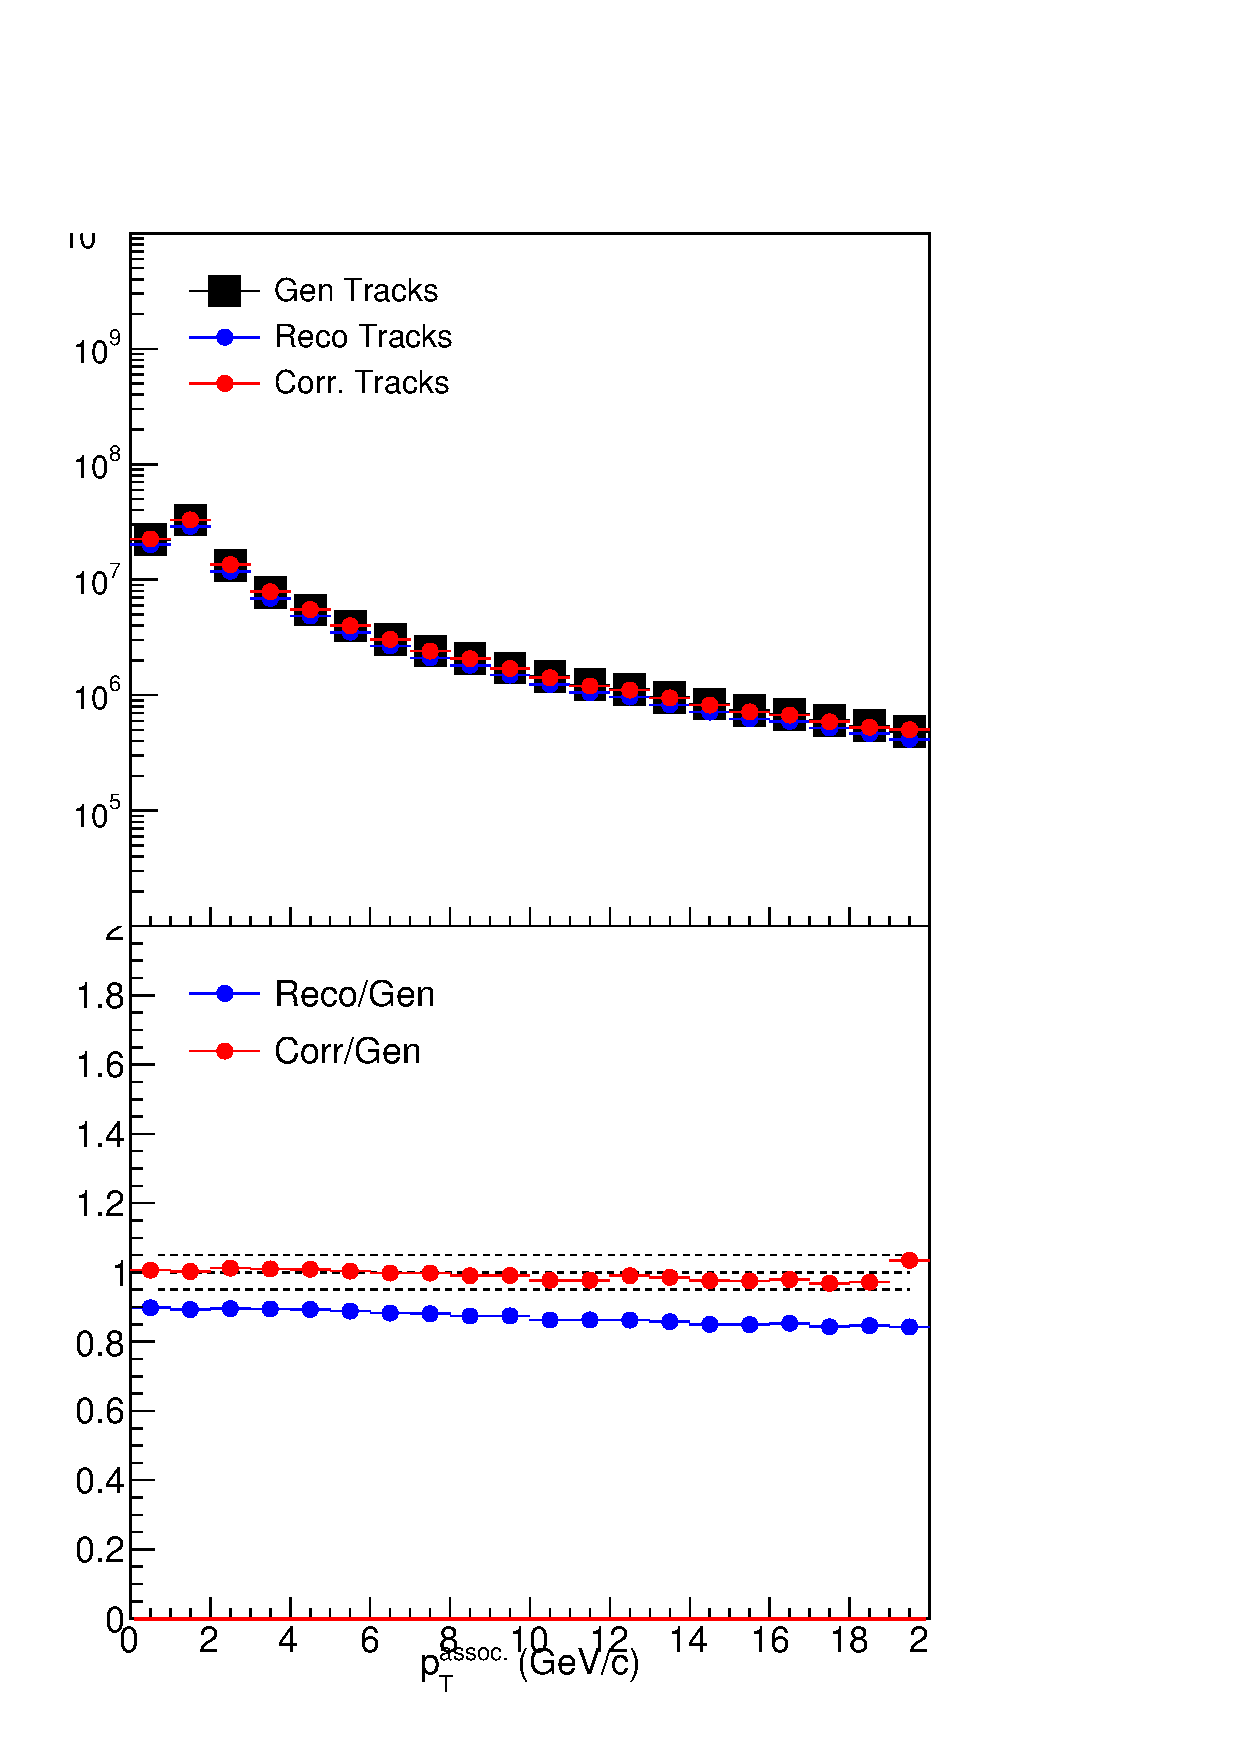
\includegraphics[width=0.3\textwidth]{figures/Detector/TrackingEfficiencyPtPythia.pdf}
             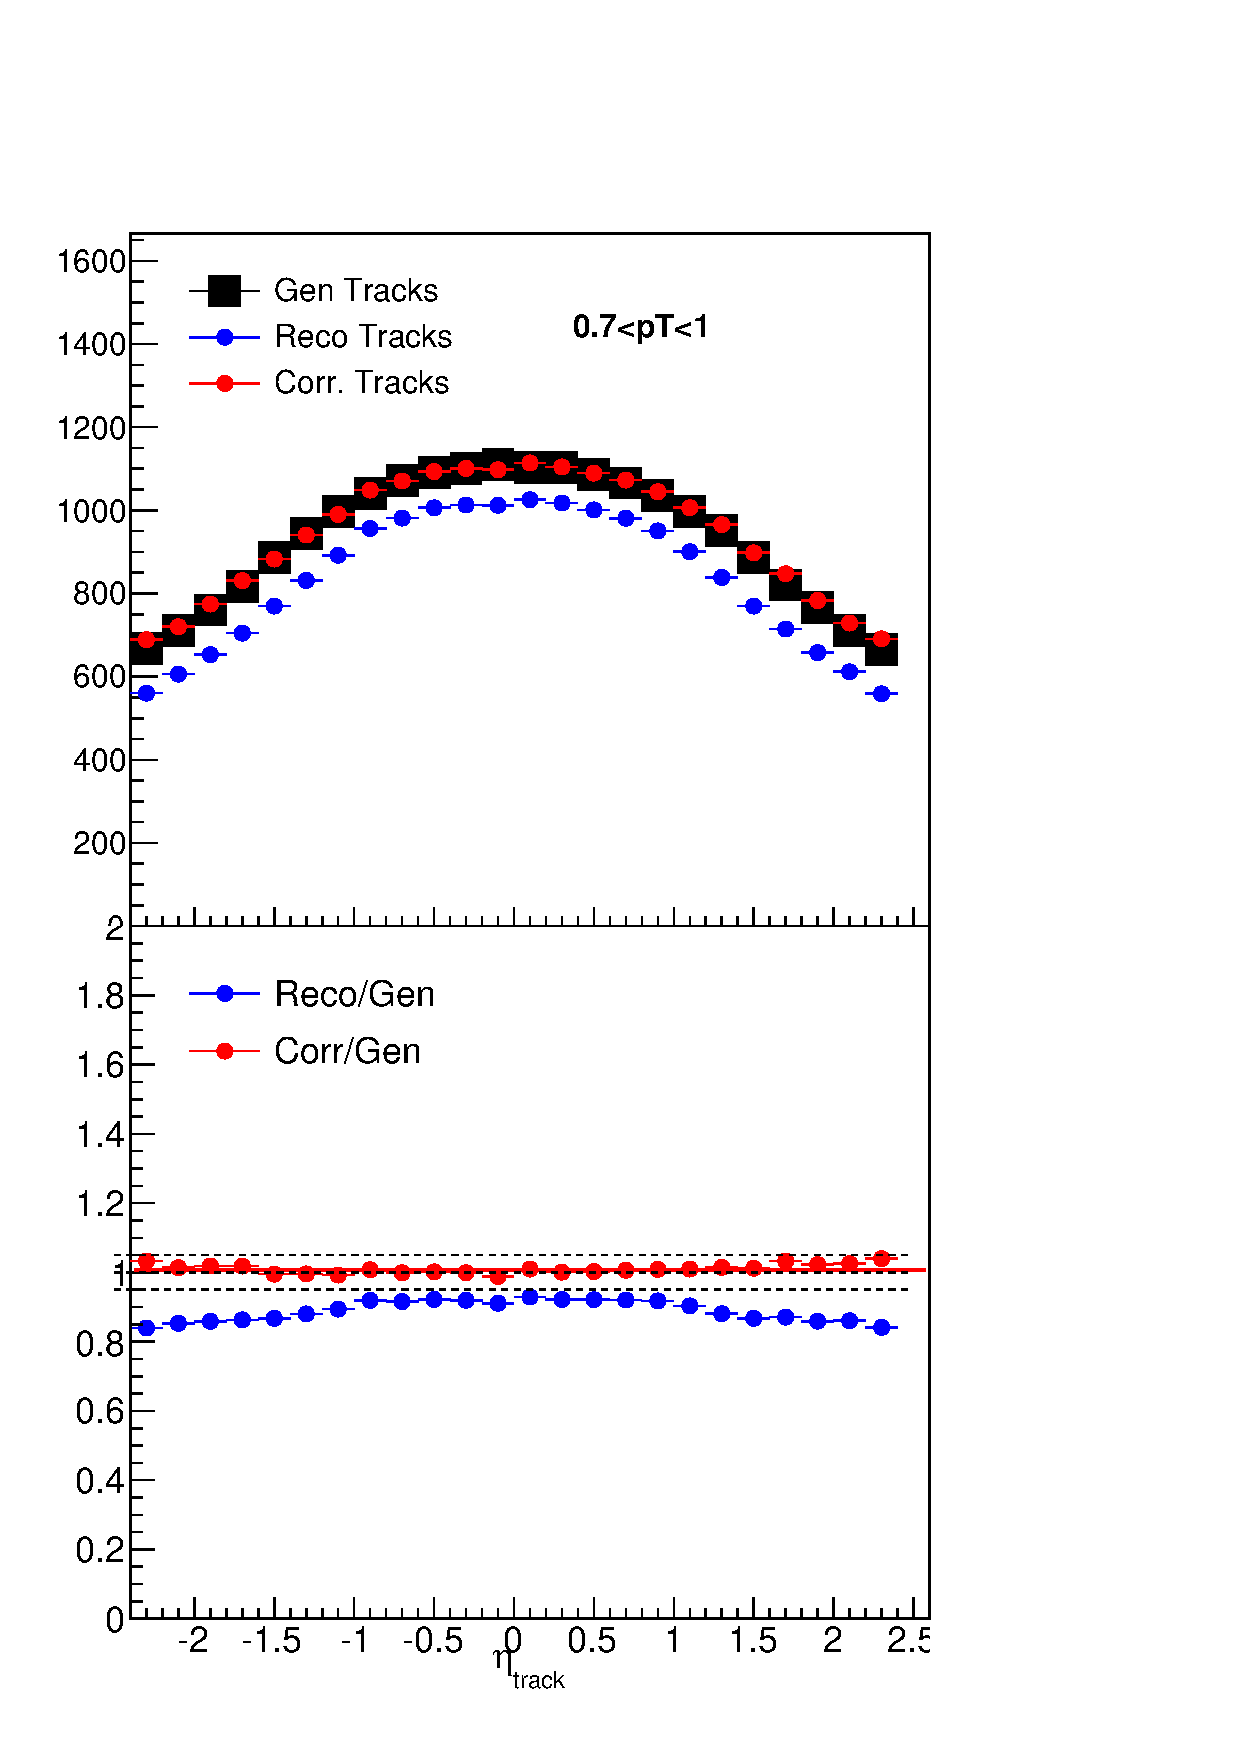
\includegraphics[width=0.3\textwidth]{figures/Detector/TrackingEfficiencyEtaPythia_TrkPt0p7TrkPt1.pdf}	
                    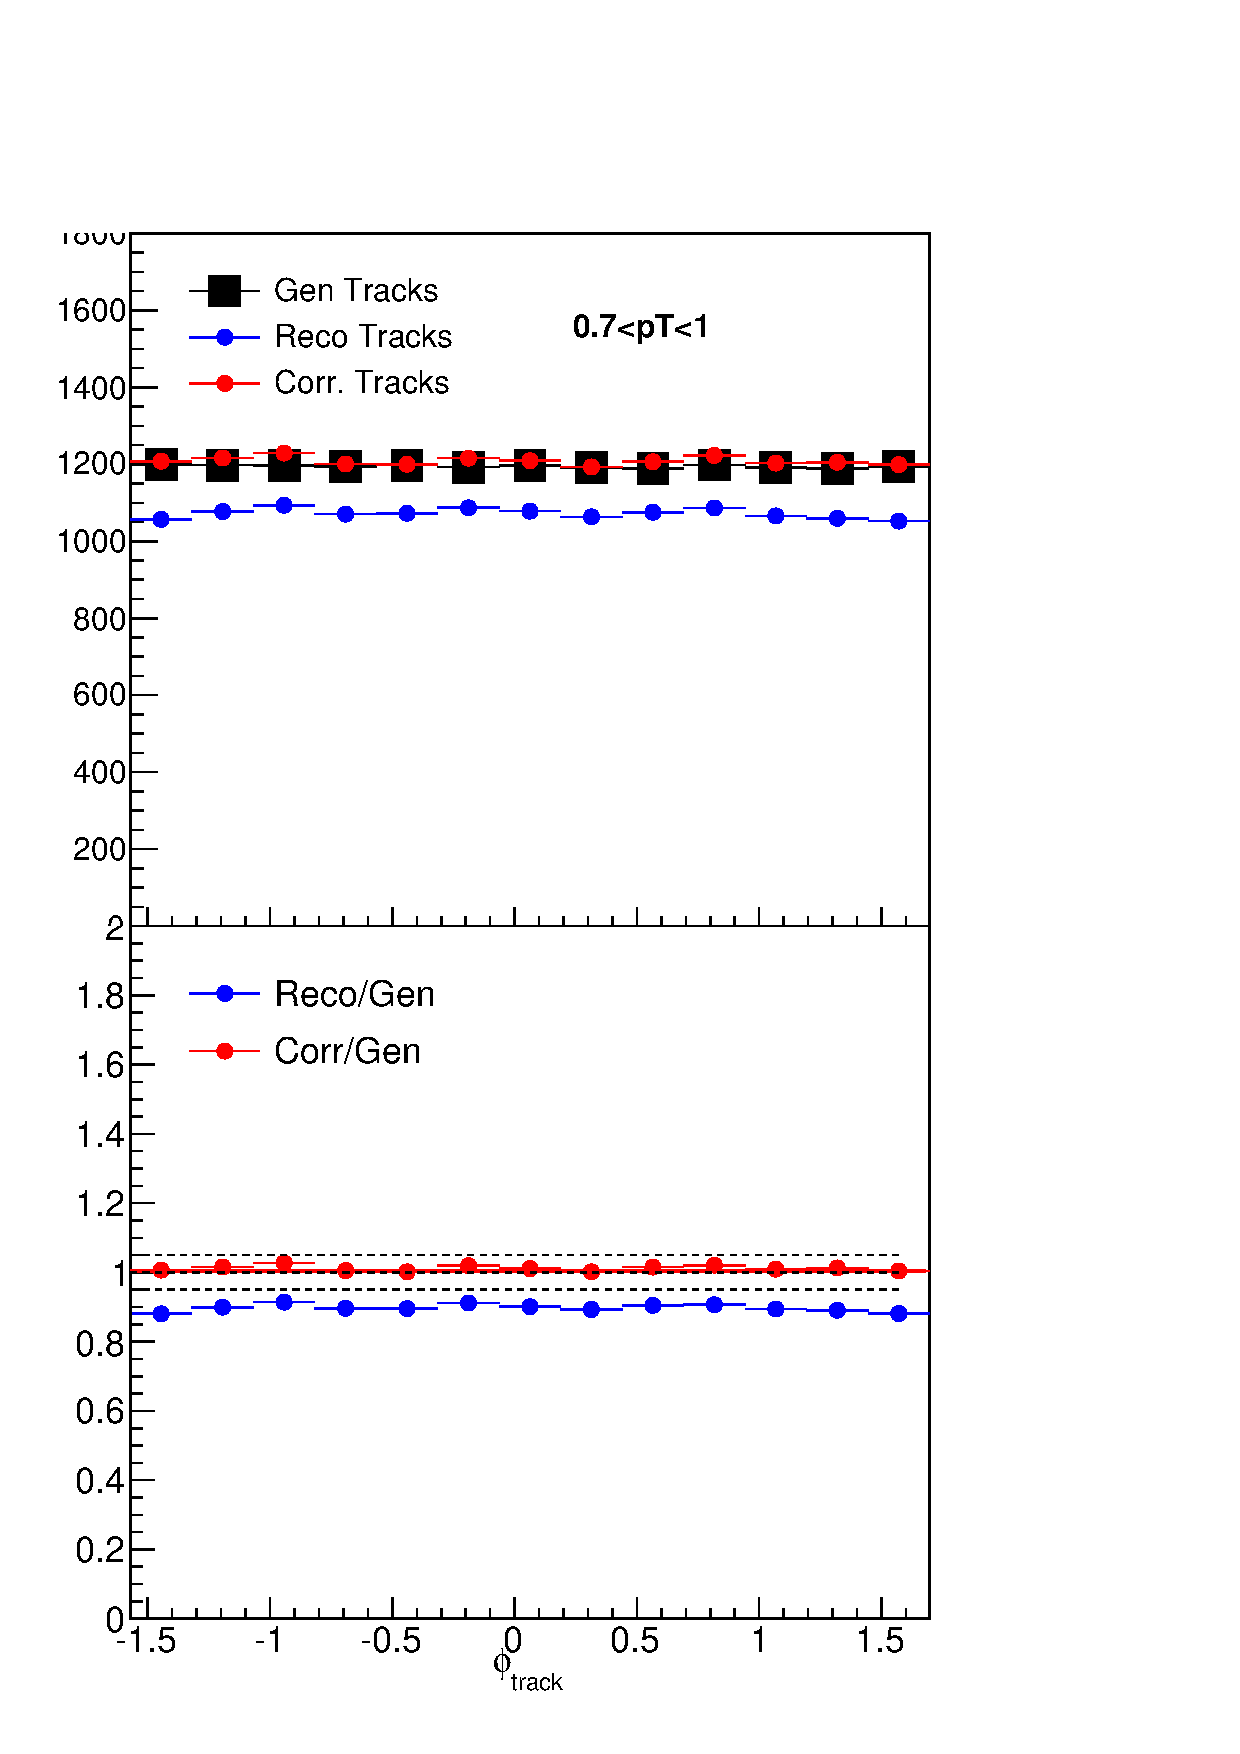
\includegraphics[width=0.3\textwidth]{figures/Detector/TrackingEfficiencyPhiPythia_TrkPt0p7TrkPt1.pdf}	
         \caption[Tracking efficiency correction example]{Tracking efficiency correction closure for {\sc pythia} simulation at 5.02 TeV, comparing tracking generated tracks to uncorrected and corrected reconstructed tracks, as a function of track $p_{\rm T}$ and of pseudorapidity, and azimuth for the lowest $p_{\rm T}^{\rm trk}$ bin.}
       \label{fig:trk_eff_pythia}
    \end{center}
 \end{figure}
 
 




\clearpage

\section{Jet reconstruction and correction}
\label{sec:Jets}
\subsection{Jet reconstruction with the anti-$k_{t}$ algorithm}

The goal in jet reconstruction is to identify clusters of hadrons originating from a fragmenting high-energy parton.  In high-$p_{\rm T}$ jet studies in pp collisions, the general locations of jets in an event may be qualitatively obvious via large energy deposits in calorimeters;  however, there is no clear single standard of how jet boundaries should be drawn.  In practice, jets are defined by the algorithms used to find and determine their direction.  These algorithms fall in two primary categories:  ``cone algorithms,'' which define jets within specific conical regions (based on the fact that hadronization has little effect total momentum flow), and ``sequential recombination algorithms,'' which iteratively identify and cluster pairs of closest particles to form jets that are not necessarily conical.~\cite{Salam:2009jx, bib_antikt, Cacciari:fastjet1}.  Several properties are desireable, from theoretical and experimental perspectives, in jet finding: 
\begin{itemize}
\item Straightforward implementation for both theoretical calculations and jet-finding and reconstruction in experimental measurements
\item Cross-sections that are finite in perturbation theory
\item Infrared and collinear (IRC) safety -- the property that a soft collinear emission in a parton splitting should not modify the overall collection of hard (high-$p_{\rm T}$) jets in the event, in particular avoiding the possibility of non-cancelling divergences in perturbation calculations
\item Soft resilience -- clustering jets that are reasonably regular and not overly sensitive to soft particles, a property motivated by the finite resolution of experimental detectors.
\end{itemize}

\noindent Heavy ion jet studies in CMS use the anti-$k_{t}$ algorithm, a soft-resilent, IRC safe, and straightforward sequential recombination algorithm~\cite{bib_antikt}, implemented in the FastJet framework~\cite{Cacciari:fastjet1}.  The anti-$k_{t}$ algorithm clusters entities (calorimeter towers, particles, or partially clustered pseudo-jets) $i$ and $j$ based on the distance measures $d_{ij}$ between the two particles and $d_{iB}$ between the particle and beam, with the measures defined as: 

\begin{equation}
\label{eq:a_kt1}
d_{ij} = {\rm min}(k_{ti}^{-2},k_{tj}^{-2})\frac{(\Delta R_{ij})^{2}}{R^{2}}, 
\end{equation}

\begin{equation}
\label{eq:a_kt2}
d_{iB} = k_{ti}^{-2},
\end{equation}

\noindent where $k_{ti}$ refers to the transverse momentum of particle $i$, $\Delta R_{ij}$ refers to the spatial distance (in rapidity and azimuth) between the two particles, and radius parameter $R$ is a reconstruction parameter.  The name anti-$k_{t}$ derives from the negative exponent for $k_{t}$ (in contrast to other sequential recombination algorithms), which enables IRC safety and soft resilience by making jet shape sensitivity to a particle inversely correlated to the particle's transverse momentum.  With this low sensitivity to soft particles, the anti-$k_{t}$ algorithm results in a collection of mostly circular jets (except in the case of jets separated by less than $2R$, in which each jet has a radius of $\pi R^{2}$.  The choice of parameter $R$ is a trade-off between capturing more fragmentation products (as can extend as far as $\Delta R{ij}$ = 0.8 in pp collisions), and limiting the influence of background particles in jet reconstruction.  In heavy ion experimental studies, where background levels are very high, typical choices of R range from 0.2 to 0.5.  

With the CMS detector, jets may be clustered from ECAL and HCAL information only (``calorimeter jets'') or from information from the full detector, using the particle flow (PF) algorithm.  The PF algorithm improves jet energy resolution (JER) substantially at low-$p_{\rm T}$ (at 10 GeV JER is 15\% for PF jets versus 40\% for calorimeter jets) with improvements decreasing for higher-$p_{\rm T}$ jets (at 100 GeV PF jet JER is 8\% versus 12\% for calorimeter jets, falling to a difference of 4\% versus 5\% at 1 TeV).  For jet-track correlation studies, however, the resolution improvements that the particle flow algorithm offers come at the cost of enhancing sensitivity to tracking biases in the jet-track correlation signal, since low-$p_{\rm T}$ tracks are included in jet reconstruction.  In this analysis, calorimeter jets are used to avoid these auto-correlation effects, and because we will consider jets with $p_{\rm T} > 120$ GeV for which calorimeter jet energy resolution is adequate.  Jets are reconstructed with anti-$k_{t}$ radius $R = 0.3$ for 2.76 TeV data (``ak3Calo'' jets), and with radius $R = 0.4$ for 5.02 TeV data (``ak4Calo'' jets).  In pp data at 2.76 TeV and 5.02 TeV the contribution to the jet energy from the underlying event (UE) is negligible (less than 1 GeV), so no underlying event subtraction is employed.
 
 
\subsection{Underlying event subtraction in PbPb data}

In PbPb collisions it is necessary to subtract contributions from the large underlying event in order to recover the true jet energy.  There are a variety of methods used for underlying event subtraction, of which the following two are relevant for this anlaysis.  

\subsubsection{Noise/pedestal subtraction}
 In most CMS high-$p_{\rm T}$ jet analyses, including 5.02 TeV PbPb data studies here, underlying event subtraction is performed using a variant of an iterative noise/pedestal subtraction technique~\cite{Kodolova:2007hd}.  This algorithm occurs in the following steps: 
 \begin{itemize}
 \item First, the mean ``pedestal'' energy in calorimeter cells as a function of energy $\eta$ ($P(\eta)$) is calculated along with its dispersion.  
 \item The pedestal function $P(\eta)$ is subtracted from all cells.  
 \item Cells with non-physical negative energy entries are then set to zero.
 \item $ \langle{\rm E_{cell}}\rangle + \langle\sigma (\rm E_{cell})\rangle$ is subtracted from each cell to compensate for the elimination of negative energy cells.
 \item Jets are clustered from the pedestal-subtracted cells using the anti-$k_{t}$ algorithm.  
 \item The pedestal function $P(\eta)$ is then re-derived using only cells that are not a part of clustered jets, and the algorithm is repeated.  
 \end{itemize}
 
 \noindent  After this underlying event subtraction is applied, the anti-$k_{t}$ algorithm with radius parameter $R = 0.4$ is then employed for jet reconstruction (``akPu4Calo jets'').  

\subsubsection{HF/Voronoi subtraction}
For 2.76 TeV PbPb data a different algorithm, designed to eliminate the threshold and possible resulting bias from the noise/pedestal technique, is employed~\cite{AN_2014_024}.  This algorithm uses information from the HF detector to model and subtract the underlying event using Voronoi decomposition (``HF/Voronoi'' algorithm) in the following steps: 
\begin{itemize}
\item The distribution of underyling $E_{\rm T}$ as a function of $\eta$ and $\phi$ is modeled using singular value decomposition (SVD) training (${\rm d}p_{\rm T}/{\rm d}\eta / {\rm }\phi$ with Voronoi parameters $v_{1}...v_{4}$) to extrapolate the UE distribution from the HF calorimeter at large $\eta$ to the central analysis region ($|\eta| < 1.6$).
\item The modeled UE distribution is subtracted from all calorimeter cells.
\item Each calorimeter cell is associated with its nearest neighbors, and energy is redistributed between neighboring in an ``equalization'' procedure used to eliminate non-physical negative $E_{\rm T}$ entries (optimized to minimize energy transfers.
\end{itemize}

\noindent After Voronoi subtraction and equalization, the anti-$k_{t}$ algorithm is employed with radius parameter $R = 0.3$ to cluster (``akVs3Calo") jets.

\subsection{Jet energy corrections}
\label{sec:JEC}

Jet reconstruction as described above gives spatial coordinates and $p_{\rm T}$ for each jet as measured by the detector.  Our goal in jet studies, however, is to reconstruct the true total parton or particle energy.  This is achieved through jet energy corrections (JEC) that establish a mapping between measured energy (which does not, for example, include neutrinos produced in jet fragmentation) and ``true'' jet energies.  This mapping is complicated by nonlinearity in detector response.  Initial corrections are derived as a function of $p_{\rm T}$ and $\eta$ using dijet QCD samples of {\sc pythia} and {\sc pythia+hydjet} Monte Carlo, spatially matching reconstructed jets to generated particles, and comparing generated versus reconstructed jet energy for these matched jets.  These ``MC truth'' corrections are applied to measured jet energies to return a collection of jets that, on average, capture the kinematic distribution of the partons before fragmentation.

These corrections do not, however, fully account for the non-linearity of calorimeter response.  In particular, in an effect particularly relevant for jet-track correlation studies, the jet energy scale depends on jet fragmenation.  Given two jets with identical parton energy, the jet with softer fragmentation (i.e. jets with a higher fraction low-$p_{\rm T}$ particles) will be on average reconstructed with lower energy than the jet with harder fragmentation.  When combined wtih a jet selection threshold, this non-linearity results in a bias that systematically underestimates the jets with soft fragmentation in the analysis sample.  An additional fragmentation-function dependent jet energy correction (JFF-JEC) is therefore applied after initial jet energy corrections in order to reduce this bias (detailed in Ref.~\cite{AN_2014_024}).  These JFF-JEC are derived using the number of particle flow candidates ($N_{\rm PF}$) in the jet with $p_{\rm T} > 2$ GeV, with this threshold chosen to reduce the influence of soft fluctuations in the underlying event.   Correction tables are derived as a function of $N_{\rm PF}$, jet $p_{\rm T}$, and PbPb event centrality in {\sc pythia} and {\sc pythia+hydjet} simulation, and are applied to jets after the JECs described above.  Finally, iterative residual corrections are applied as a function of jet $p_{\rm T}$.  The application of JFF-JECs reduces the overall quark/gluon non-closure, as illustrated for PbPb data in Fig.~\ref{fig:quark_gluon}, and slightly improves jet energy resolution overall.

\begin{figure}[hbtp]
\begin{center}
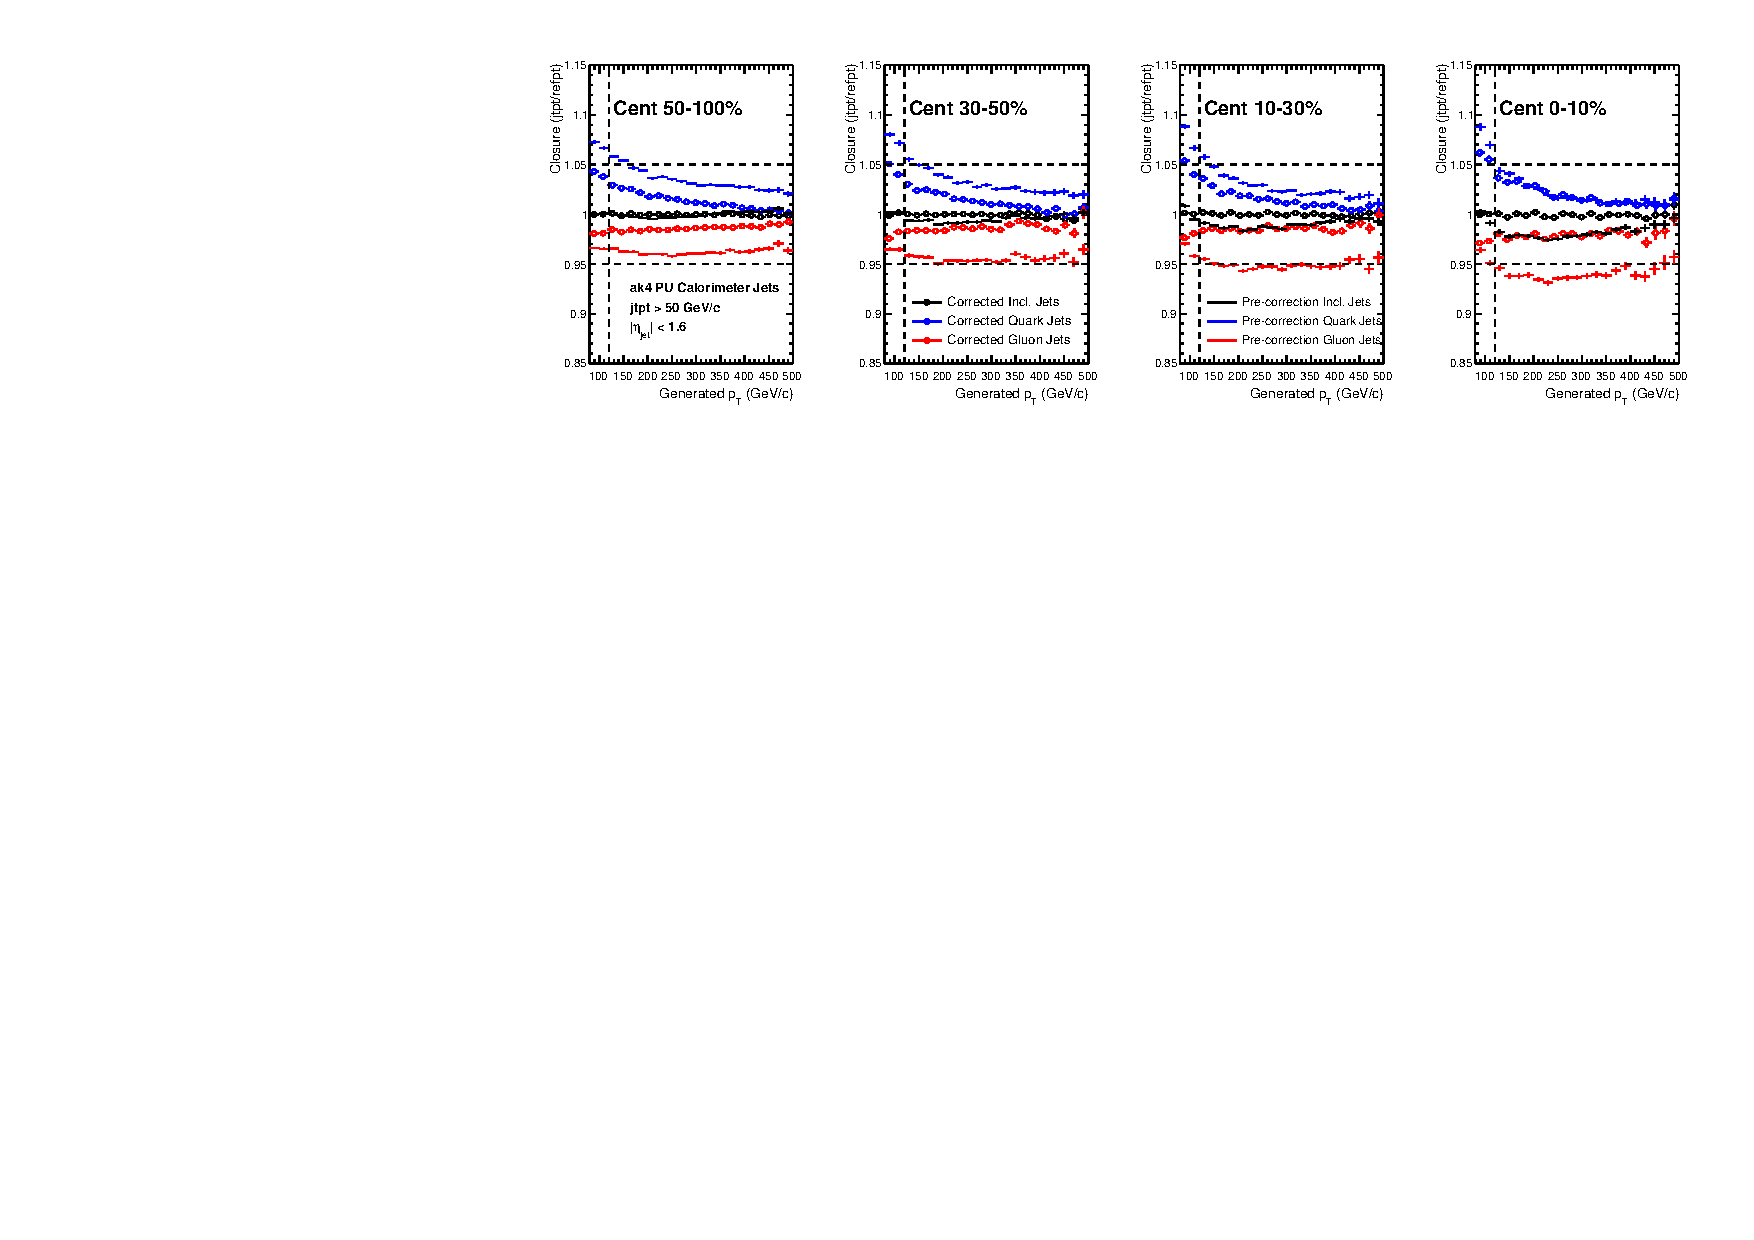
\includegraphics[width=0.99\textwidth]{figures/Detector/fullClosures_DogaIterative_centDep_correctToJetPt.pdf}
\caption{Closure with and without JFF-JEC for quark and gluon jets.}
\label{fig:quark_gluon}
\end{center}
\end{figure}



\clearpage

\section{Data and Monte Carlo samples}
\label{sec:Samples}
\subsection{Data samples and event selection}

This analysis is based on PbPb and pp data collected with the CMS detector at 2.76 TeV and 5.02 TeV during Run 1 and Run 2 of the CERN LHC.  Studies at 2.76 TeV use 166 $\mu {\rm b}^{-1}$ of PbPb data collected in 2011, and 5.3 pb$^{-1}$ of pp data collected in 2013.  Studies at 5.02 TeV use 404 $\mu {\rm b}^{-1}$ of PbPb data and 25 pb$^{-1}$ of pp data, both collected in 2015.  Online collision selection was performed using the CMS HLT described in Sec.~\ref{sec:HLT} to obtain a minimum bias sample of PbPb collision events, and to obtain samples of PbPb and pp data with the requirement that events contain at least one high-$p_{\rm T}$ jet (with $p_{\rm T} > 80$~GeV for pp data and 2.76 TeV PbPb data, $p_{\rm T} > 100$~GeV for 5.02 TeV PbPb data).  These jet triggers are fully efficient for offline-reconstructed jets with $p_{\rm T} > 120$~GeV.  Total numbers of selected events are summarized in Table~\ref{table:evt_sel}.

\begin{table}[h!]
\begin{center} 
\caption{Summary of data samples and number of selected events}
\label{table:evt_sel} 
\begin{tabular}{|c|c|c|c|}
\hline
\hline
Dataset & Number of selected events  \\
\hline
\hline
2.76 TeV PbPb MinimumBias & 1.01 M \\
2.76 TeV PbPb Jet-triggered ($p_{\rm T} > 80$~GeV) & 1.25 M \\
2.76 TeV pp Jet-triggered ($p_{\rm T} > 80$~GeV) & 1.27 M \\
\hline
\hline
5.02 TeV PbPb MinimumBias & 764 k \\
5.02 TeV PbPb Jet-triggered ($p_{\rm T} > 100$~GeV) & 3.35 M \\
5.02 TeV pp Jet-triggered ($p_{\rm T} > 80$~GeV) & 2.66 M\\
\hline
\hline
\end{tabular}
\end{center} 
\end{table} 

A number of quality cuts are applied, as is standard for CMS analyses to remove detector noise backgrounds, ultra-peripheral collisions, beam gas events, and events with exceptionally large pixel occupancy. These selection criteria have shown to have negligible impact on dijet analyses~\cite{Chatrchyan:2012gt,Chatrchyan:2012gw}, and are as follows in PbPb and pp collisions: 
\begin{itemize}
\item Vertex-z position within 15 cm of the center of the detector ($|\rm v_{z}| < 15$)
\item Primary vertex filter -- a requirement that events include a reconstructed primary vertex filter with at least two tracks, requiring the presence of inelastic hadronic scattering and removing beam-gas events and ultra-peripheral collisions
\item Beam-scraping filter -- a requirement of pixel clusters compatible with the primary vertex.  In pp, this requires that if there are more than 10 tracks, at least 25\% of tracks must be highPurity (see Sec.~\ref{sec:Tracks})
\item HB/HE noise filter -- a filter to exclude events exhibiting uncharacteristic calorimeter noise~\cite{Chatrchyan:2009hy}
\item PbPb data only:  HF coincidence filter -- at least 3~GeV recorded in at least each of at least three hadronic forward calorimeter towers on each side of the interaction point
\end{itemize}

\noindent These cleaning cuts are applied to both minimum bias and jet-triggered data samples.  Additional event selection will later be applied to obtain samples of high-$p_{\rm T}$ jets and dijet events, as discussed in Sec.~\ref{sec:jet_sel} below. 



\subsection{Collision centrality determination and classes}
\label{sec:centrality}

The variable centrality is used to parameterize the degree of overlap of the colliding nuclei.  In CMS, centrality is determined using total transverse energy ($E_{\rm T}$) in the HF calorimeter towers, in the region $4.0 < |\eta| < 5.2$.  The distribution of total $E_{\rm T}$ in all events is used to divide the total minimum bias event sample into centrality bins, each containing 0.5\% of the total events.  The resulting centrality distribution is flat in minimum bias data by construction.  In jet-triggered data, however, requiring the presence of a high-$p_{\rm T}$ jet results in a larger fraction of more central collisions (in which hard-scatterings are more likely).  The collisions defined as ``most central'' (centrality = 0\%) are those with the greatest $E_{\rm T}$, corresponding to collisions in which the nuclei collided head-on.  In contrast, the collisions defined as ``least central'' or ``most peripheral'' (centrality = 100\%) are those in which the nuclei barely overlapped at all.  To observe how jet modifications evolve with changing centrality, this analysis considers four centrality classes:  0-10\% (most central), 10-30\%, 30-50\%, and 50-100\%.

\subsection{Monte Carlo simulation}

Monte Carlo (MC) simulation is used in this analysis to evaluate and correct for jet reconstruction performance and tracking efficiency for both pp and PbPb data.  Simulation of pp data and of the hard processes in PbPb data are performed using the {\sc pythia} (version 6, tune Z2~\cite{bib_pythia}) event generator. In order to have reasonable event samples in all jet $p_{\rm T}$ ranges, different samples are produced with various cut-off values of $\hat{p_{\rm T}}$, which are then combined using their respective cross-sections as weights.  To simulate CMS detector output for MC events, {\sc geant}4 detector simulation is used~\cite{bib_geant}.  Jet and track reconstruction performance and efficiency for pp data is evaluated by comparing observables in {\sc pythia} samples as generated to the same observables after they have been passed through the detector simulation and the same reconstruction procedures applied to pp data.  For the relevant jet kinematics observables relevant to this analysis, {\sc pythia} reasonably reproduces pp data.  

For PbPb data, the underlying event is simulated using {\sc hydjet} (Drum5 tune)~\cite{Lokhtin:2005px}, which combines hydrodynamics with ``mini-jets''  produced with quenched {\sc pythia} input.  Hard processes are generated using {\sc pythia}, and are directly embedded in this {\sc hydjet} sample (refered to as {\sc pythia+hydjet} simulation), with no medium quenching effects applied to the embedded jets.  This {\sc pythia+hydjet} sample is used to evaluate the reconstruction effects of the presence of the heavy ion collision environment, $other$ than the jet-medium interactions that are our objects of study.  As for {\sc pythia} simulation of pp data, comparing {\sc pythia+hydjet} samples that have been passed through the detector and reconstructed chain to the generated Monte Carlo allows for the evaluation of jet and track reconstruction performance.  


\subsubsection{Monte Carlo centrality and vertex-z reweighting}

Simulated {\sc pythia+hydjet} samples are generated minimum bias, and therefore must be reweighted to match the bias toward more central events induced by requiring the presence of a high-$p_{\rm T}$ jets discussed in Sec.~\ref{sec:centrality}.  Reweighting factors are calculated for each 0.5\%-wide centrality bin, and applied to the {\sc pythia+hydjet} sample overall to match the PbPb centrality distribution.  Similarly, another reweighting procedure is performed to match the distributions of the position of the primary interaction along the beam direction in MC and data for both pp and PbPb collisions.  Figures~\ref{fig:HydCent_Reweighting}-\ref{fig:PythiaVz_Reweighting} illustrate the necessity and effects of these reweighting procedures.  


\begin{figure}[ht]
\begin {center}
  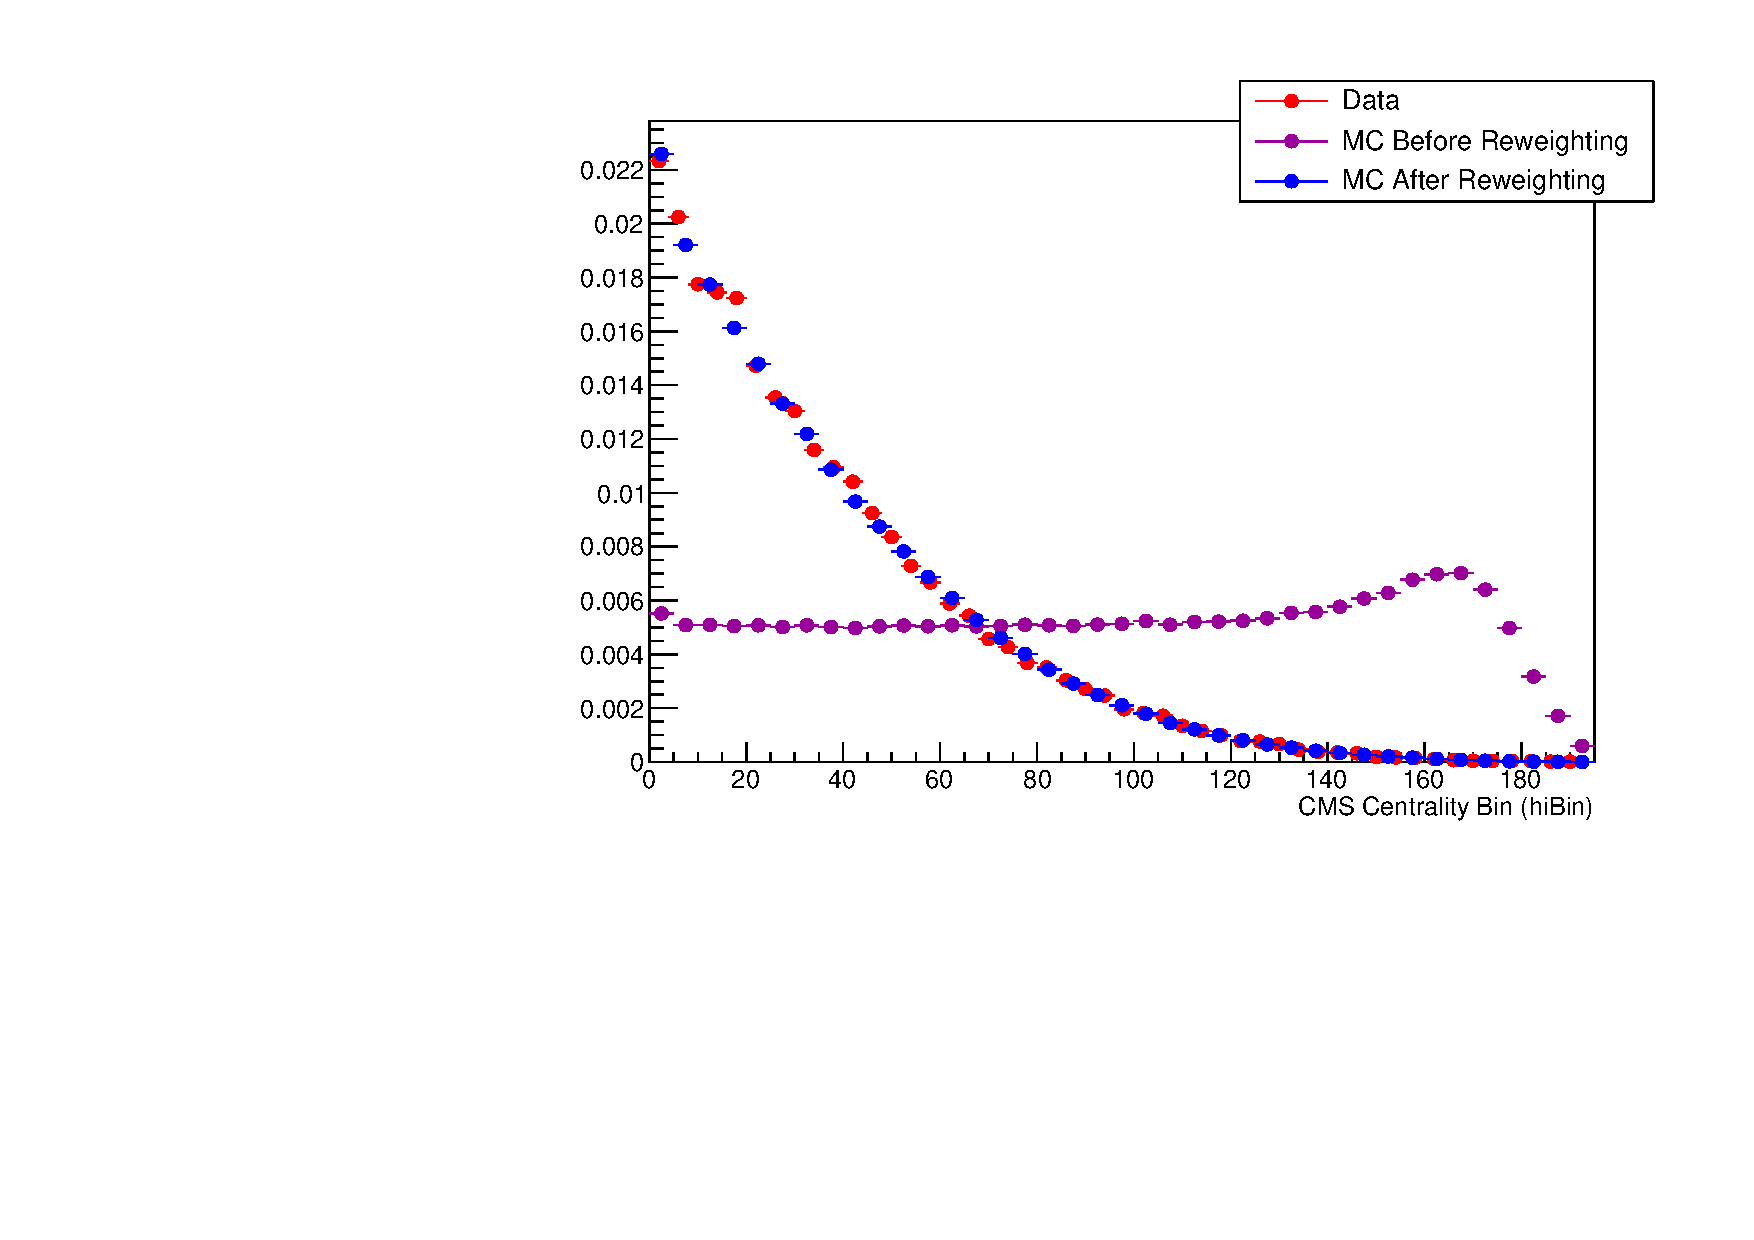
\includegraphics[width=0.58\linewidth]{figures/Samples/HydjetCentralityReweighting.pdf}
  \caption{
    Centrality distribution for {\sc pythia+hydjet} reweighted to the distribution of PbPb data.
  }
\label{fig:HydCent_Reweighting}
\end{center}
\end{figure}



\begin{figure}[ht]
\begin {center}
  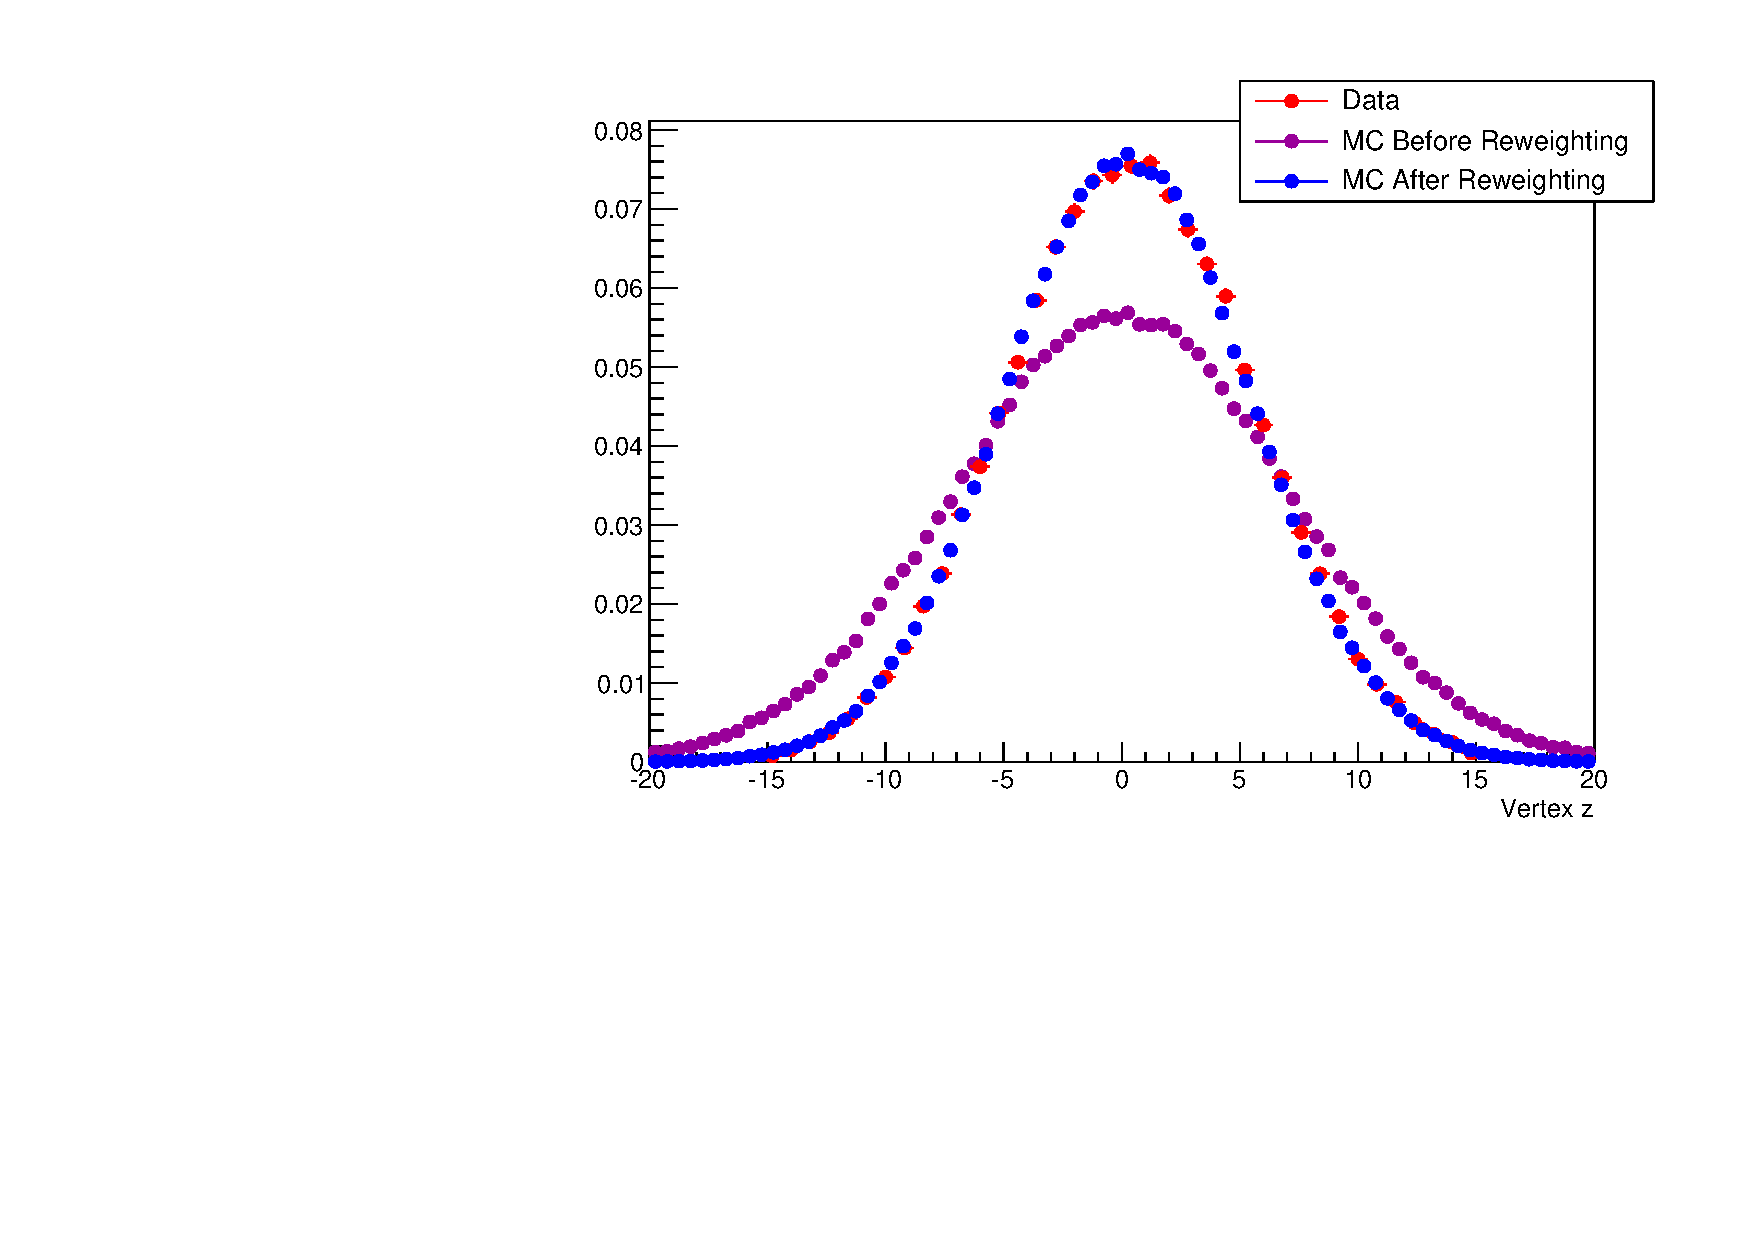
\includegraphics[width=0.58\linewidth]{figures/Samples/HydjetVzReweighting.pdf}
  \caption{
    Vertex z distribution for {\sc pythia+hydjet} reweighted to the distribution of PbPb data.
  }
\label{fig:HydVz_Reweighting}
\end{center}
\end{figure}




\begin{figure}[ht]
\begin {center}
  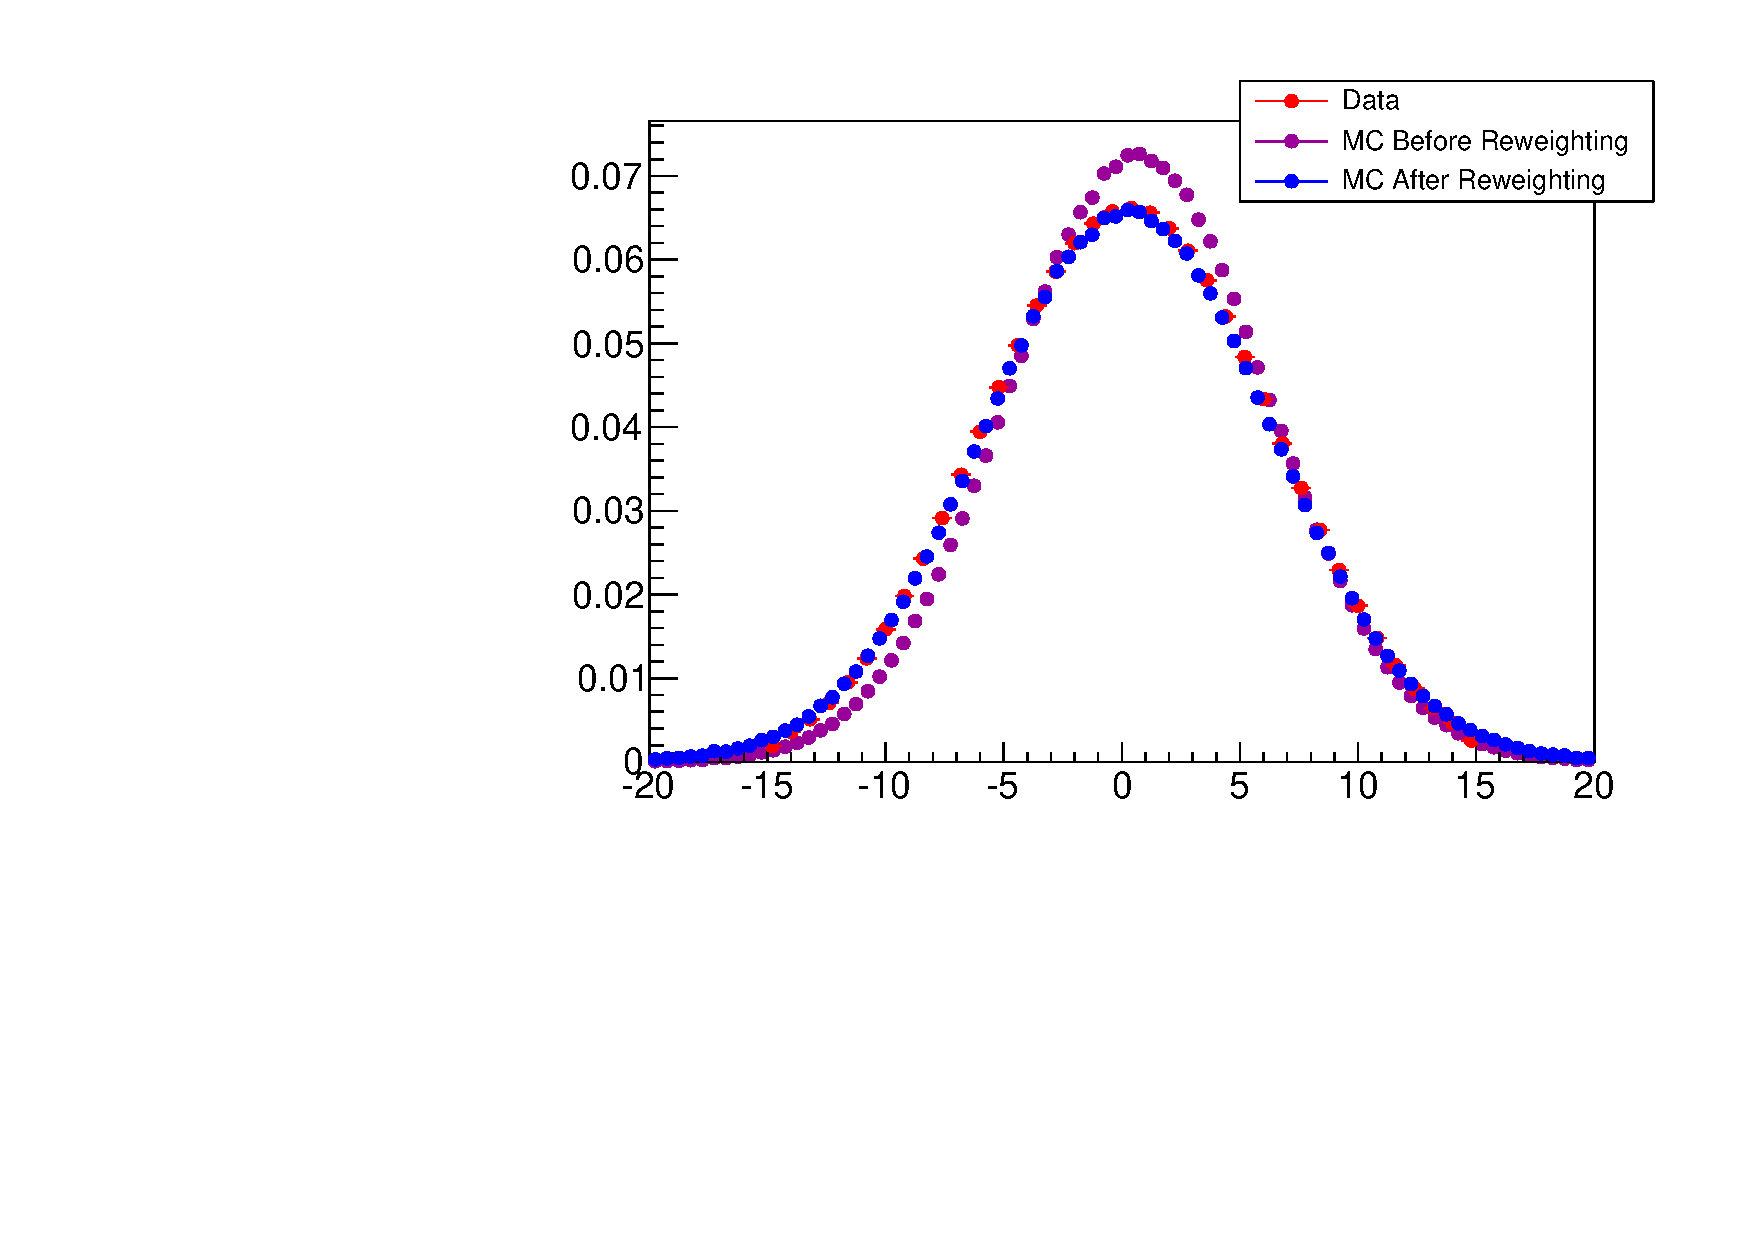
\includegraphics[width=0.58\linewidth]{figures/Samples/PythiaVzReweighting.pdf}
  \caption{
    Vertex z distribution for {\sc pythia} reweighted to the distribution of pp data.
  }
\label{fig:PythiaVz_Reweighting}
\end{center}
\end{figure}


\subsubsection{Monte Carlo samples at 2.76 TeV}

Tables~\ref{mc_stats_276}  and~\ref{mc_stats_502} summarize the {\sc pythia} and {\sc pythia+hydjet} samples used in this analysis by $\hat{p_{\rm T}}$, with respective numbers of generated events and cross-sections used for combining samples. 

\begin{table}[htbp]
\begin{center} 
\caption{Summary of Monte Carlo samples and generated events at 2.76 TeV}

\label{mc_stats_276} \begin{tabular}{|c|c|c|c|}
\hline
Generator & Process & Cross section (mb) & Number of events \\
\hline
{\sc pythia+hydjet} & $\hat{p_{\rm T}}$ $> 50$~GeV & $1.025\times 10^{-3}$ & 395k  \\
{\sc pythia+hydjet} & $\hat{p_{\rm T}}$ $> 80$~GeV & $9.865\times 10^{-5}$ & 368k  \\
{\sc pythia+hydjet} & $\hat{p_{\rm T}}$ $> 120$~GeV & $1.129 \times 10^{-5}$ & 367k \\
{\sc pythia+hydjet} & $\hat{p_{\rm T}}$ $> 170$~GeV & $1.465 \times 10^{-6}$ & 392k \\
{\sc pythia+hydjet} & $\hat{p_{\rm T}}$ $> 220$~GeV & $2.837\times 10^{-7}$ & 181k \\
{\sc pythia+hydjet} & $\hat{p_{\rm T}}$ $> 280$~GeV & $2.837\times 10^{-7}$ & 50k \\
\hline
{\sc pythia} & $\hat{p_{\rm T}}$ $> 80$~GeV & $9.865\times 10^{-5}$ & 104k  \\
{\sc pythia} & $\hat{p_{\rm T}}$ $> 120$~GeV & $1.129 \times 10^{-5}$ & 975k \\
{\sc pythia} & $\hat{p_{\rm T}}$ $> 170$~GeV & $1.465 \times 10^{-6}$ & 69k \\

\hline
\end{tabular}
\end{center} 
\end{table} 


\clearpage

\subsubsection{Summary of Monte Carlo samples at 5.02 TeV}

\begin{table}[h!]
\begin{center} 
\caption{Summary of Monte Carlo samples and generated events at 5.02 TeV}

\label{mc_stats_502} \begin{tabular}{|c|c|c|c|}
\hline
\hline

Generator & Process & Cross section (mb) & Number of events \\
\hline
{\sc pythia+hydjet} & $\hat{p_{\rm T}}$ $> 80$~GeV/$c$ & $4.412\times 10^{-4}$ & 499k \\
{\sc pythia+hydjet} & $\hat{p_{\rm T}}$ $> 120$~GeV/$c$ & $ 6.147\times 10^{-5}$& 496k \\
{\sc pythia+hydjet} & $\hat{p_{\rm T}}$ $> 170$~GeV/$c$ &  $1.018\times 10^{-5}$ & 498k \\
{\sc pythia+hydjet} & $\hat{p_{\rm T}}$ $> 220$~GeV/$c$ &  $2.477\times 10^{-6}$ & 200k \\
{\sc pythia+hydjet} & $\hat{p_{\rm T}}$ $> 280$~GeV/$c$ &  $6.160\times 10^{-7}$ & 200k \\




\hline
{\sc pythia} & $\hat{p_{\rm T}}$ $> 80$~GeV/$c$ & $4.412\times 10^{-4}$ & 500k \\
{\sc pythia} & $\hat{p_{\rm T}}$ $> 120$~GeV/$c$ & $6.147\times 10^{-5}$& 500k \\
{\sc pythia} & $\hat{p_{\rm T}}$ $> 170$~GeV/$c$ & $1.018\times 10^{-5}$ & 499k \\
{\sc pythia} & $\hat{p_{\rm T}}$ $> 220$~GeV/$c$ & $2.477\times 10^{-6}$ & 200k \\
{\sc pythia} & $\hat{p_{\rm T}}$ $> 280$~GeV/$c$ & $6.160\times 10^{-7}$ & 200k \\


\hline
\hline

\end{tabular}
\end{center} 
\end{table} 


\clearpage


\subsection{Jet selection and dijet asymmetry classes}
\label{sec:jet_sel}

Jet selection in this analysis is restricted to the pseudorapidity region $|\eta_{\rm jet}| < 1.6$ to ensure stable reconstruction performance in the calorimeter barrel region.  A requirement is also imposed that the highest-$p_{\rm T}$ track contains no less than 1\% and no more than 98\% of the total jet $p_{\rm T}$.  In the jet selection refered to as ``inclusive jets'' for analysis at both 2.76 TeV and 5.02 TeV, all jets with $p_{\rm T, jet} > 120$~GeV are considered.  In this selection, it is possible to select more than one jet from the same event, provided that each jet satisfies the inclusive selection criteria. 

In addition to the inclusive jet selection, a ``dijet'' selection of events containing two back-to-back high-$p_{\rm T}$ jets is also analyzed for the 2.76 TeV data sample.  Events are included in this sample based on the criteria that they contain highest-$p_{\rm T}$ ``leading'' jet with $p_{\rm T,1} > 120$~GeV and a second-highest-$p_{\rm T}$ ``subleading'' jet with $p_{\rm T,2} > 50$~GeV with relative azimuthal separation between the two jets $\Delta\phi_{1,2} > \frac{5\pi}{6}$.  This dijet sample is subdivided into a sample of relatively ``balanced'' dijets, with similar $p_{\rm T,1}$ and $p_{\rm T,2}$ and a sample of relatively ``unbalanced'' dijets in which the leading jet has a much larger $p_{\rm T}$ than the subleading jet based on asymmetry parameter $A_{\rm J}$. The balanced selection is defined as those events for which $A_{\rm J} < 0.22$, while the unbalanced selection as defined as those events for which $A_{\rm J} > 0.22$.  The dividing value $A_{\rm J} = 0.22$ is chosen for consistency with previous CMS analyses~\cite{Chatrchyan:2011sx, HIN_2014_010}.  In this analysis, 52\% of central PbPb events are balanced, while 67\% of pp events are balanced.  Jet kinematics for all jet samples (broken down by asymmetry for 2.76 TeV dijet data) are shown in Appendix~\ref{app:kinematics_run1} for 2.76 TeV data and in Appendix~\ref{app:kinematics_run2} for 5.02 TeV data.

\subsection{Track selection and classes}

Tracks, reconstructed as described in Sec.~\ref{sec:Tracks} are required to satisfy the following criteria: 
\begin{itemize}
\item  $|\eta_{\rm trk}| < 2.4$ -- restricts to the barrel region of the tracker
\item  $0.5 < p_{\rm T}^{\rm trk} < 300$ GeV -- excludes very low-$p_{\rm T}$ tracks where reconstruction performance is not stable
\item High Purity criteria  -- see  Sec.~\ref{sec:high_purity}
\item Distance of closest approach (DCA) in x-y plane and in z less than 3 times the DCA error -- reduces fraction of tracks not associated with a primary vertex
\item Relative $p_{\rm T}^{\rm trk}$ error less than 30\% (10\% for 5.02 TeV PbPb data) -- removes tracks with very poor resolution (has a negligible effect on efficiency as CMS resolution is generally good) 
\end{itemize}

\noindent For 5.02 TeV PbPb data, the following additional criteria are also applied to reduce the contribution from misidentified tracks~\cite{AN-15-187}:
\begin{itemize}
\item Exclude tracks with fewer than 11 tracker hits
\item Require that for each track the chi-squared over number of degrees of freedom ($\chi^{2}$/ Ndof) of the track fit, also divided by the number of tracker layers (nLayer) hit as the track passed through the detector, is less than 0.15, i.e. $\chi^{2}$/Ndof/nLayer $< 0.15$.  
\item For tracks with $p_{\rm T} > 20$ GeV (the kinematic region in which misreconstruction is difficult to access with Monte Carlo), calorimeter matching is applied:  since high-$p_{\rm T}$ tracks eventually deposit their energy in a calorimeter after passing through the tracker, tracks are required to be associated with calorimeter transverse energy $E_{\rm T} = (E_{\rm ECAL} + E_{\rm HCAL})/\rm{cosh}(\eta_{\rm trk})$, such that $E_{\rm T} > 0.5 p_{\rm T}^{\rm trk}$ 

\end{itemize}

\noindent After these selection criteria are applied, tracking efficiency corrections are applied as described in Sec.~\ref{sec:track_eff}.  Tracks in this analysis are considered in the following classes:  0.5--1~GeV, 1--2~GeV, 2--3~GeV, 3--4~GeV, 4--8~GeV, 8--12~GeV, 12--16~GeV, 16--20~GeV, and above 20~GeV.   Not all bins are considered in every analysis, and for 5.02 TeV studies the lowest-$p_{\rm T}^{\rm trk}$ bin is 0.7--1~GeV.     

\clearpage

\subsection{Summary of analysis bins}

Table~\ref{table:bins} summarizes the key kinematic selections and bins for the three components to this analysis.  In all cases, identical selection is applied to PbPb and pp data.  Event, jet, and track quality cuts are not included in this table.

\begin{table}[h!]

\begin{center} 
\caption{Summary of data selections and analysis bins}
\label{table:bins} 
\begin{tabular}{|p{0.6in}|p{1.4in}|p{1.4in}|p{1.4in}|}
\hline
\hline
Variable & 2.76 TeV Inclusive & 5.02 TeV Inclusive & 2.76 TeV Dijets\\
\hline
PbPb & 0-10\%, 10-30\%,  & 0-10\%, 10-30\%, & 0-10\%, 10-30\%,\\
Centrality & 30-50\%, 50-100\% & 30-50\%, 50-100\% & 30-50\%, 50-100\%\\
\hline
Jet & $|\eta_{\rm jet}| < 1.6$ &  $|\eta_{\rm jet}| < 1.6$ &  $|\eta_{\rm jet}| < 1.6$ \\ 
Selection& $p_{\rm T} > $120~GeV & $p_{\rm T} > 120$~GeV & $p_{\rm T,1} > 120$~GeV\\
 &&&$p_{\rm T,2} > 50 $GeV\\
 &&&$\Delta\phi_{1,2}> \frac{5\pi}{6}$\\
 \hline
 $A_{\rm J}$ Bins & -- & -- &  $A_{\rm J} < 0.22$, \\
 &&&$A_{\rm J} > 0.22$\\
 \hline
 Track $\eta$ & $|\eta_{\rm trk}| < 2.4$ &$|\eta_{\rm trk}| < 2.4$ & $|\eta_{\rm trk}| < 2.4$ \\
 \hline
 $p_{\rm T}^{\rm trk}$ Bins & 1-2~GeV, 2-3~GeV, 3-4~GeV, 4-8~GeV & 0.7-1~GeV, 1-2~GeV, 2-3~GeV, 3-4~GeV, 4-8~GeV & 0.5-1~GeV, 1-2~GeV, 2-3~GeV, 3-4~GeV, 4-8~GeV, 8-300~GeV\\

\hline
\hline
\end{tabular}
\end{center} 
\end{table} 




\clearpage


\section{Jet-track correlation measurements}
\label{sec:JetTrack}

\subsection{Analysis procedure}

Measurements in this analysis are carried out by considering correlations between high-$p_{\rm T}$ jets and tracks in PbPb and pp collisions.  Jets are selected within $\eta < 1.6$ and $p_{\rm T}$ above a particular threshold.  For each jet, the relative separation in pseudorapidity ($\Delta\eta = \eta_{\rm track} - \eta_{jet}$) and azimuth ($\Delta\eta = \phi_{\rm track} - \phi_{jet}$) is measured between the jet and all charged-hadron tracks within $\eta < 2.4$.  For each jet-track pair, these measurements are recorded in a two-dimensional $\Delta\eta - \Delta\phi$ correlation in a particular track transverse momentum ($p_{\rm T}^{\rm trk}$) and centrality class.  Each correlation is normalized by dividing by the number of jets in the sample ($N_{\rm jets}$), resulting in a signal pair distribution, $S(\Delta\eta,\Delta\phi)$, that gives the per-jet yield of tracks and their relative distance from the jet:

  \begin{equation}
  \label{eq:signal}
  S(\Delta\eta,\Delta\phi) = \frac{1}{N_{\rm jets}}\frac{\rm d^{2} N^{\rm same}}{\rm d\Delta\eta d\Delta\phi}.
  \end{equation}

This procedure results in a two dimensional measurement of the distribution of charged tracks with respect to the jet axis.  The same procedure may also be repeated, weighting each track by its $p_{\rm T}^{\rm trk}$, in order to obtain a distribution of transverse momentum with respect to the jet axis.  These particle density and $p_{\rm T}^{\rm trk}$ correlations form the basis for all results discussed in this analysis.  From this point, several additional corrections and other steps are necessary to isolate jet-related effects from long range and uncorrelated backgrounds.  These additional steps are as follows: 
\begin{itemize}
\item A correction for jet-track pair acceptance effects;
\item Separation of correlations into short-range jet peaks and and long range components;
\item Monte Carlo-based corrections for biases related to jet reconstruction.
\end{itemize}
After these steps, a range of different observables may be extracted to characterize the multiplicity and distribution of tracks and $p_{\rm T}^{\rm trk}$ at both small and large angles from the jet axis.  

\clearpage

\subsection{Jet-track correlation pair-acceptance correction}

This analysis considers $\Delta\eta$ jet-track separations as large as $\Delta\eta = 2.5$.  With finite $\eta$ acceptance for both jets and tracks ($|\eta_{\rm jet}| < 1.6$ and $|\eta_{\rm track}| < 2.4$, tracks that fall within $\Delta\eta = 2.5$ of a jet may be outside the tracking acceptance.  This pair acceptance effect results in trapezoidal correlations that fall with rising $|\Delta\eta|$ as tracks are ``lost'' outside of the acceptance.  This effect is purely geometric, and may be corrected by reproducing this pair acceptance geometry.  This is done by creating a ``mixed event'' correlation in which jets in the sample are correlated to tracks within $|\eta| < 2.4$ from randomly selected events in a minimum bias PbPb sample, matched in vertex-$z$ position (within 0.5 cm) and centrality (within 2.5\%).  This reproduces the pair acceptance geometry from the signal correlations: 
  
  \begin{equation}
  \label{eq:background}
  ME(\Delta\eta,\Delta\phi) = \frac{1}{N_{\rm jets}}\frac{\rm d^{2}N^{\rm mix}}{\rm d\Delta\eta d\Delta\phi},
  \end{equation}
  is constructed to account for pair-acceptance effects, with $N^{\rm mix}$ denoting the number of mixed-event jet-track pairs.  The mixed event correction is normalized to unity at $\Delta\eta$=0, where the jet and track are colinear in $\eta$ and therefore have perfect pair acceptance, with the normalization factor $ME(0,0)$.  Dividing the signal correlation $S(\Delta\eta,\Delta\phi)$, defined in Equation~\ref{eq:signal}, by this normalized mixed event correlation $ME(\Delta\eta,\Delta\phi)$/$ME(0,0)$ yields the corrected per-jet correlated yield distribution, as illustrated in Figure~\ref{fig:ME_corr}: 

  \begin{equation}
  \label{2pcorr_incl}
  \frac{1}{N_{\rm jets}}\frac{\rm d^{2} N}{\rm d\Delta\eta\, \rm d\Delta\phi}
  = \frac{ME(0,0)}{ME(\Delta\eta,\Delta\phi)}\times S(\Delta\eta,\Delta\phi).
  \end{equation}
  
\begin{figure}[ht!] 
\begin{center} 
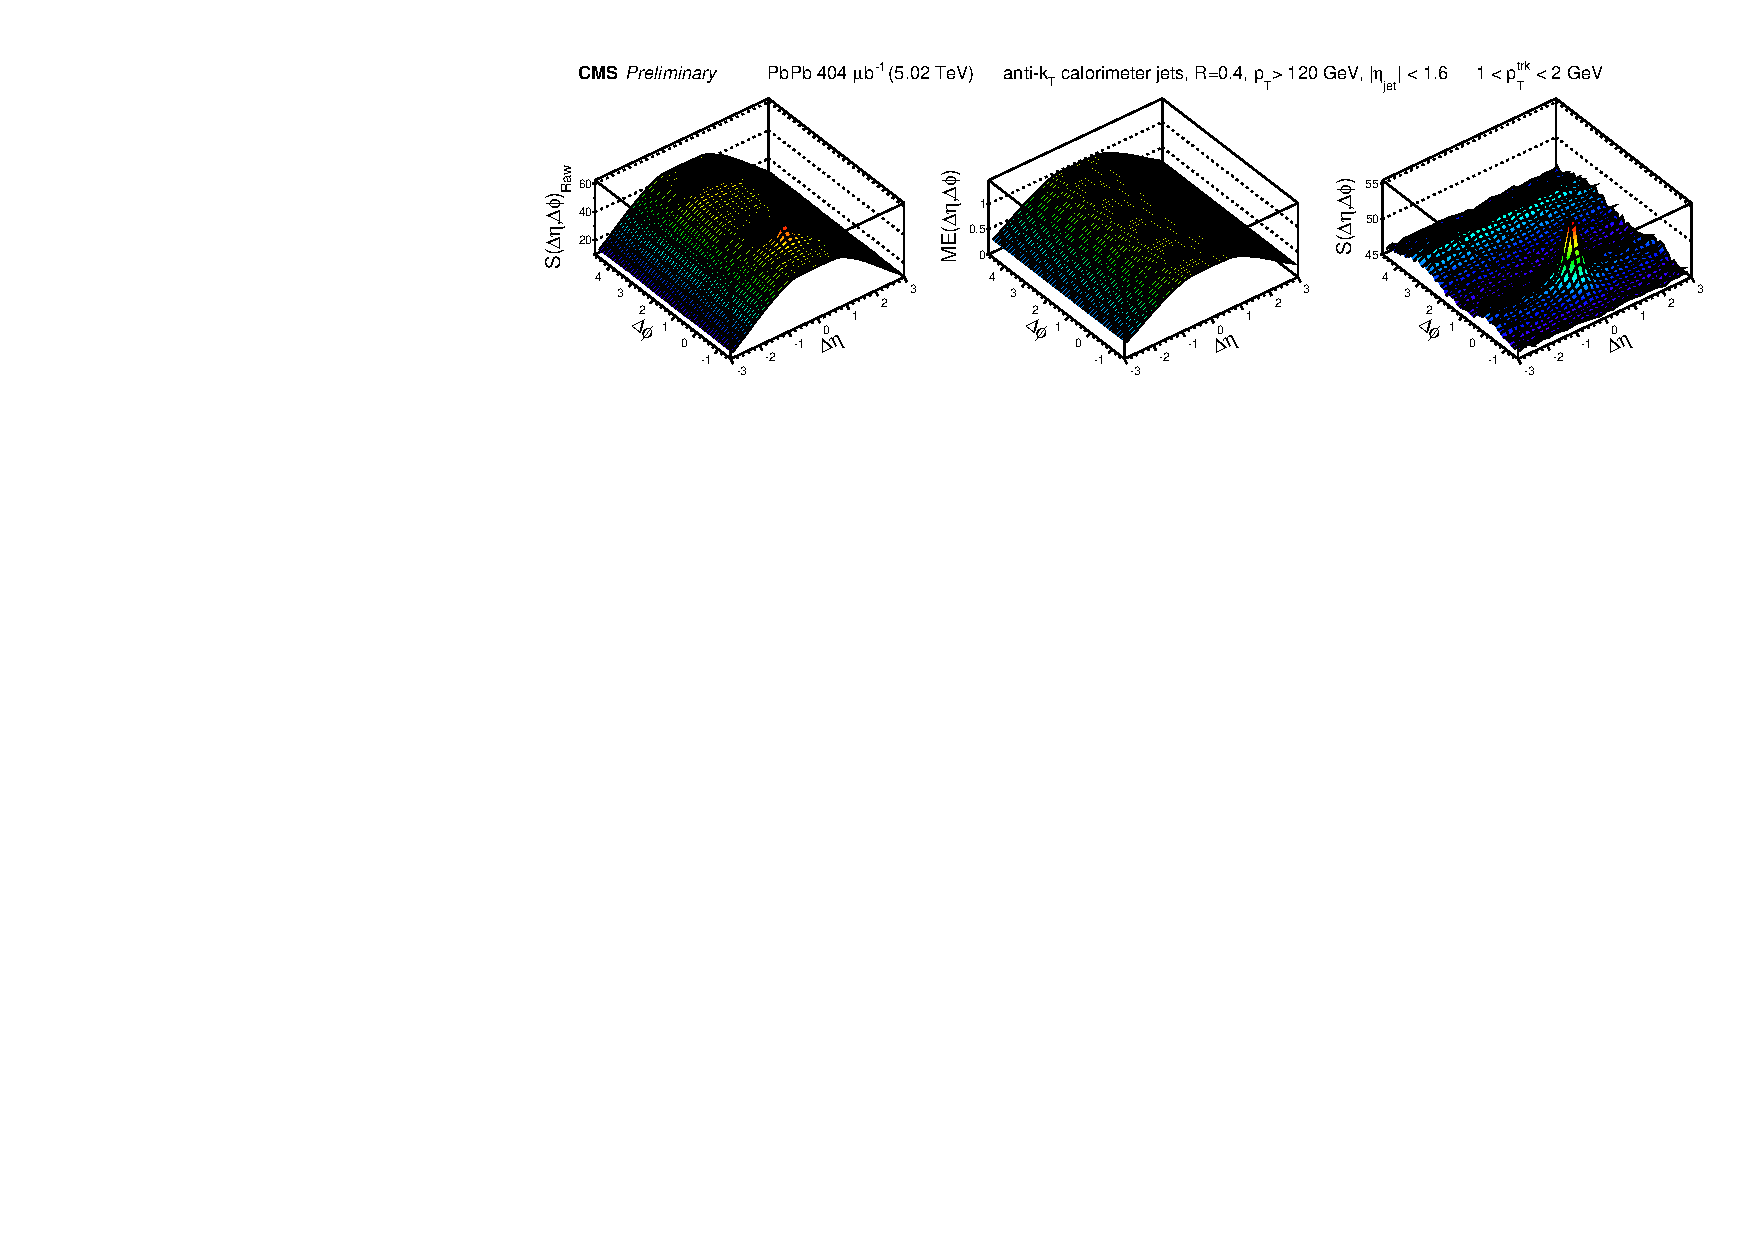
\includegraphics[width=0.99\textwidth]{figures/Results/ME_Correction.pdf}
\caption[Illustration of the pair-acceptance correction procedure]{Illustration of the pair-acceptance correction procedure:  left panel shows signal correlation $S(\Delta\eta,\Delta\phi)$, and center panel shows mixed event correlation $ME(\Delta\eta,\Delta\phi)$.  Dividing the signal correlation by the normalized mixed event correlation yields the corrected per-jet correlated yield distribution shown in the right panel.}
\label{fig:ME_corr}
\end{center} 
\end{figure} 

  
\subsection{Separation of correlations into long range and short-range components}
\label{sec:bkg_sub}

After correlations are corrected for pair-acceptance effects, in each correlation we are left with a well-defined jet peak sitting at $\Delta\eta = 0$, $\Delta\phi = 0$ on top of a large combinatoric and long range correlated background.  For most measurements, it is necessary to isolate this jet peak in order to distinguish jet-related effects from eventwise correlations.   In order to achieve this, we note that the long range correlation is independent of $\Delta\eta$ at distances larger than $\Delta\eta = 1.5$ from the jet.  This ``sideband'' region ($1.5 < |\Delta\eta| < 3.0$) is used to model the underlying event, capturing both the level of the combinatoric background in the event, and also the long range ``flow'' correlations in the event.  The assumption of rapidity--independence of the flow harmonics is based on the CMS study~\cite{v2_HIN_11_012}, which shows no appreciable variation of the elliptic flow for charged particles above 1~GeV in the pseudorapidity interval of $\Delta\eta < 3.0$ relevant for this study.  As long range correlations depend only on $\Delta\phi$, the sideband region is projected into $\Delta\phi$ to obtain a one-dimensional model of the underlying event.   To subtract this long range correlation in 2D, this distribution may be either directly re-propagated into $\Delta\phi$ (as shown in Figure~\ref{fig:BG_sub1}), or may be fit in $\Delta\phi$ before repropagation in a smoothing procedure as shown in Fig.~\ref{fig:BG_sub2}.  When aiming to simply remove the long range correlated background, we fit long range correlations function modeling harmonic flow plus a term to capture the (Gaussian or sharper) ``away-side'' peak opposite the jet in relative azimuth:  

\begin{equation}
\label{eq:bkg_fit_as}
B(\Delta\phi) = B_{0}(1+2V_{\rm1}\cos{(\Delta\phi)}+2V_{\rm 2}\cos{(2\Delta\phi)}+2V_{\rm 3}\cos{(3\Delta\phi)})+A_{\rm AS}\exp{\bigg(-\bigg(\frac{|\Delta\phi-\pi|}{\alpha}\bigg)^{\beta} \bigg) },
\end{equation}

\noindent In this case, the fit is performed only as a smoothing procedure to model the background under the near-side jet peak.; as only the jet peak within $|\Delta\phi|<\frac{\pi/}{2}$ is studied, the fit to the away-side peak is not relevant to the analysis.  Furthermore, no physics conclusions can be extracted from the $V_{n}$ terms in this fit, which are used only to establish a reasonable functional form for smooth modeling of the background distributions.  

\begin{figure}[t!] 
\begin{center} 
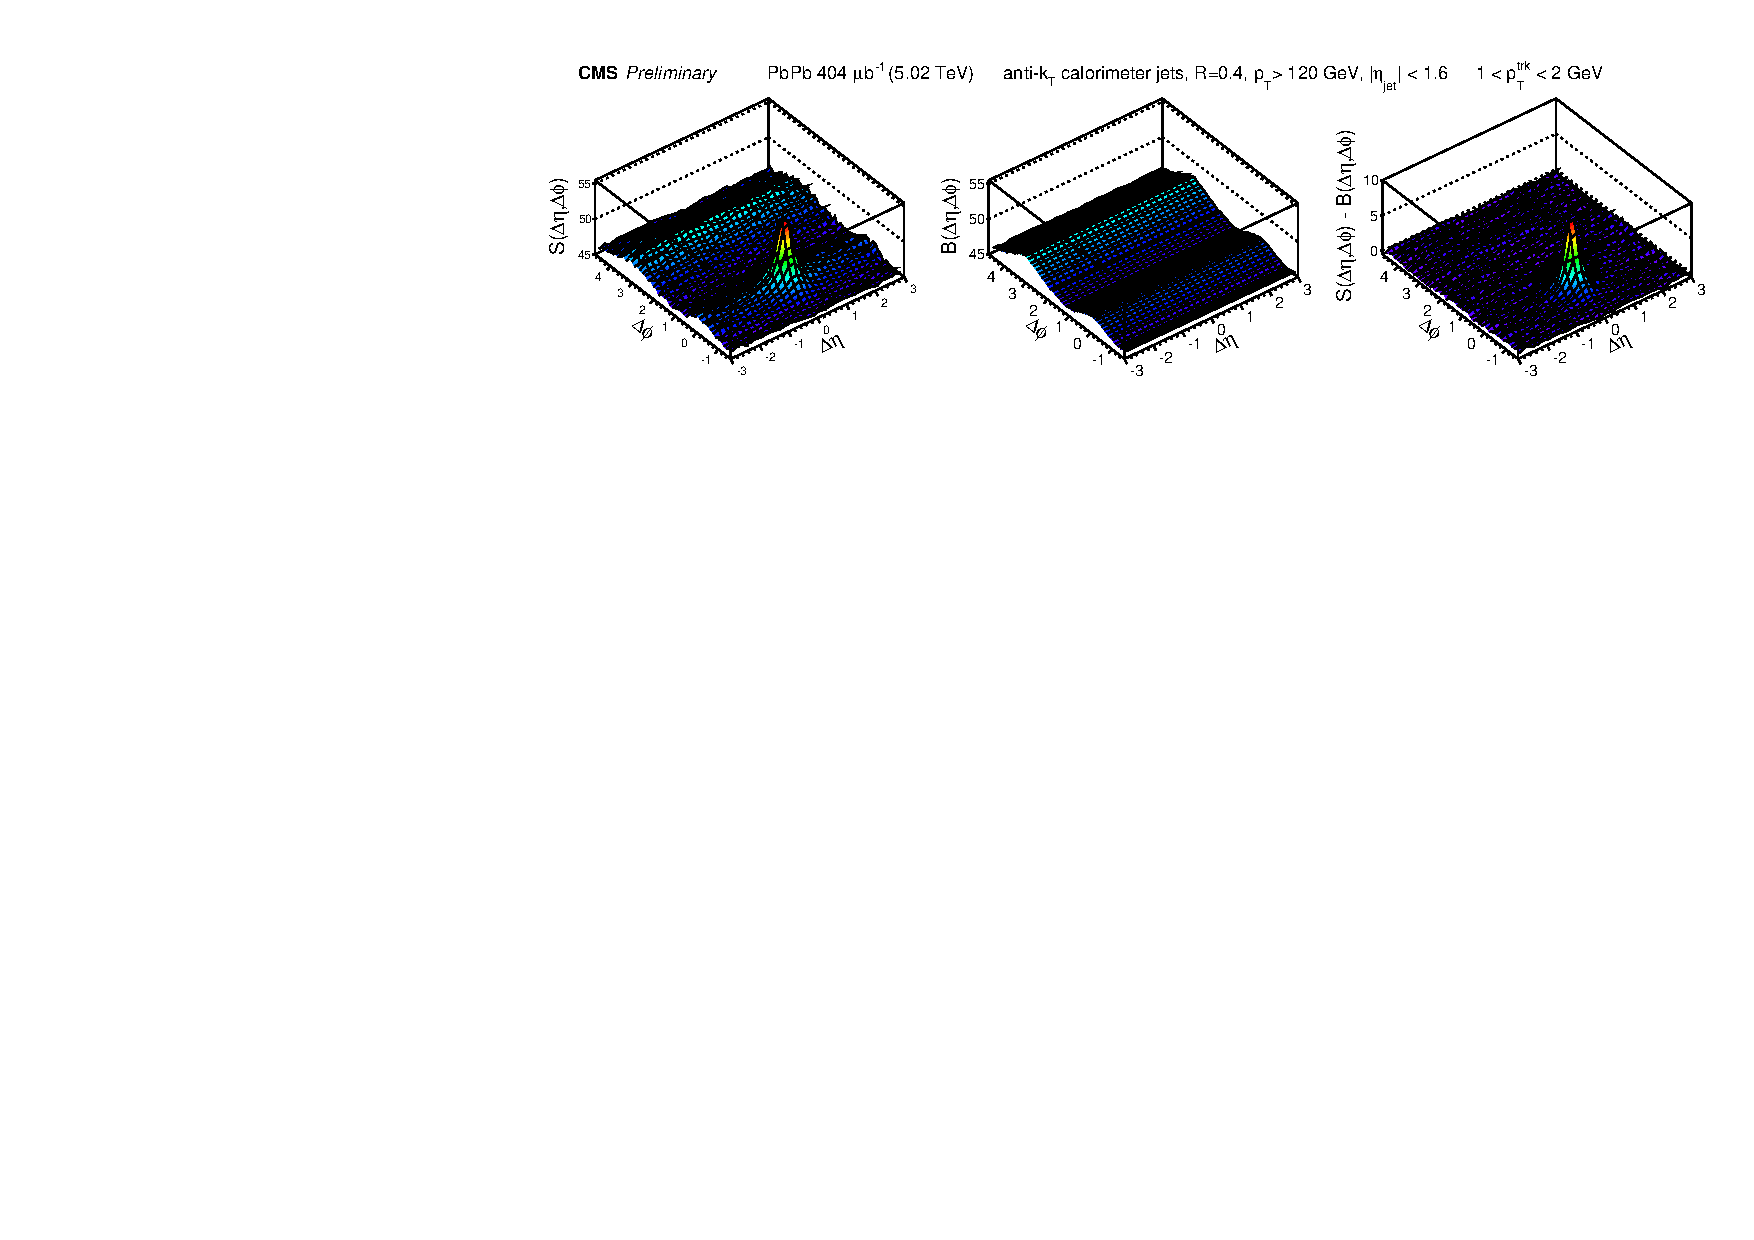
\includegraphics[width=0.99\textwidth]{figures/Results/Background_Subtraction.pdf}
\caption[Illustration of the event decomposition procedure without $\Delta\phi$ fitting]{Illustration of the event decomposition procedure without $\Delta\phi$ fitting:  left panel shows the acceptance-corrected correlation, middle panel shows the projected and re-propagated long range distribution, and right panel shows the background-subtracted jet peak.}
\label{fig:BG_sub1}
\end{center} 
\end{figure}

\begin{figure}[hbt] 
\begin{center} 
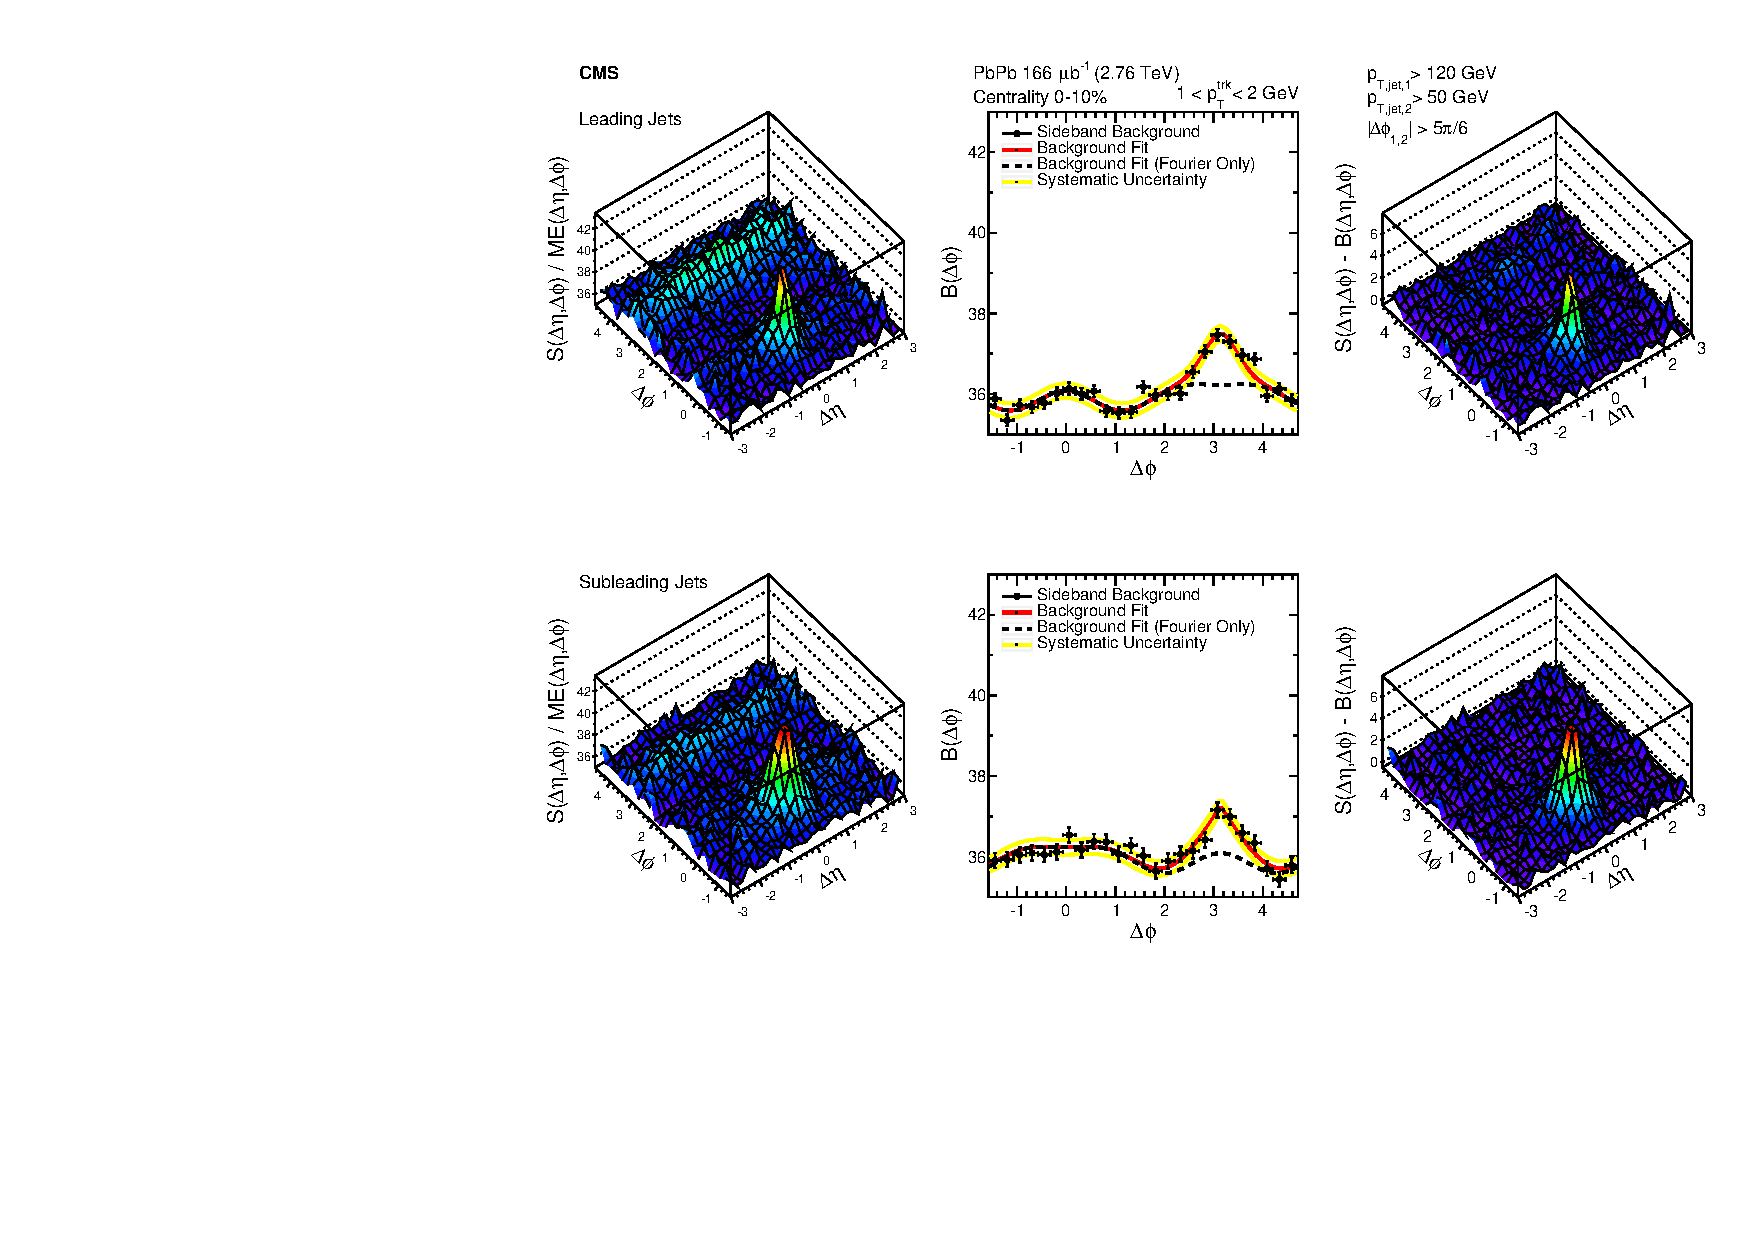
\includegraphics[width=0.99\textwidth]{figures/Results/PAS_Figure_2_TrkPt1_TrkPt2.pdf}
\caption[Illustration of the event decomposition procedure with $\Delta\phi$ fitting]{Illustration of the event decomposition procedure with $\Delta\phi$ fitting:  left panel shows the acceptance-corrected correlation, middle panel shows the projected and fit long range distribution, and right panel shows the background-subtracted jet peak.}
\label{fig:BG_sub2}
\end{center} 
\end{figure}


The long range correlations in the underlying event are in themselves interesting objects of study, however, as they contain information about the collective behavior of particles in the event as a whole, and the extent to which the distribution of high-$p_{\rm T}$ jets in the event couple to this collective flow.  To further study the long range correlations, we may apply the well-established harmonic flow decomposition method used to study two-particle correlations~\cite{Chatrchyan:2012wg} to correlations between jets and tracks.  In dijet studies, more accurate information about long range flow correlations can furthermore be obtained by making use of the fact that for our dijet selection and a given value of $\Delta\eta$ the region $-\frac{\pi}{2}<\Delta\phi<\frac{\pi}{2}$ of the leading correlation is by definition equivalent to the region $\frac{\pi}{2}<\Delta\phi<3\frac{\pi}{2}$ of the subleading correlation.  This provides a full $2\pi$ distribution of the long range correlated underlying event under both the leading and subleading jet peaks.  We can then perform a single fit to the combined background.  Here we fit with harmonic flow terms only:  

\begin{equation}
\label{eq:bkg_fit_dijet}
B(\Delta\phi)^{\rm Dijet} = B_{0}(1+2V_{\rm1}\cos{(\Delta\phi)}+2V_{\rm 2}\cos{(2\Delta\phi)}+2V_{\rm 3}\cos{(3\Delta\phi)}),
\end{equation}

\noindent In this fit, we find that terms through $\rm V_{3}$ are necessary to describe the low-$p_{\rm T}$, central background, while at higher-$p_{\rm T}$ only $\rm V_{1}$, $\rm V_ {2}$.  From this combined fit, we extract parameters $\rm V_{1}$, $\rm V_ {2}$, and $\rm V_{3}$.  Then, to better constrain the background under the signal and minimize the effects of random background fluctuations, we apply the factorization relation of overall Fourier harmonic $\rm V_{2} = v_{2}^{jet} \times v_{2}^{trk}$~\cite{Aamodt:2011by, Chatrchyan:2011eka}. The values of $\rm v_{2}^{trk}$ for charged particles are determined in Ref.~\cite{Chatrchyan:2012wg}, while the fit parameter $\rm v_{2}$ is expected to be independent of  $p_{\rm T}^{\rm trk}$ ranges for a given centrality class.  The average value of $\rm v_{2}^{jet}$ from each $p_{\rm T}^{\rm trk}$ range is calculated, and used to fix the $\rm V_{2}$ parameter on the second iteration of the fit.  Both the combined dijet fit with $B(\Delta\phi)^{\rm Dijet}$ and the final $B(\Delta\phi)$ fits are shown in Appendix~\ref{app:bkg_fits}.  Through this process, we characterize the underlying event and note that the distribution of jets as well as tracks couples to the flow modulation of the underlying event.  This has immediate consequences for studies of momentum balance between leading and subleading hemispheres of the event:  as there are non-zero contributions from odd harmonics to the long-range correlated backgrounds, we cannot expect flow cancellation when directly subtracting hemishpere $p_{\rm T}^{trk}$ distributions.  

For jet peak studies the underlying event is a background to subtracted to isolate jet peaks.  After this is done, either by direct subtraction or by subtracting the fit and re-propagated background, we are left with isolated 2D jet peaks.  Before extracting observables, we must carefully consider and correct for reconstruction biases affecting these correlated yields.  Before correlations are constructed, both tracks and jets are corrected for detector efficiencies and other reconstruction effects, as discussed in detail in Sec.~\ref{sec:Tracks} and Sec.~\ref{sec:Jets}, respectively.  There are two additional effects, however, in which jet biases are coupled to the multiplicity of low-$p_{\rm T}$ tracks:  a bias against reconstructing jets with soft fragmentation that arises from nonlinearity in calorimeter response (reduced but not eliminated by the JFF-JEC described in Sec.~\ref{sec:JEC}), and a bias toward selecting jets that sit on upward (soft) fluctuations in the background resulting in excess low-$p_{\rm T}$ yields around the jet axis.  Both effects are studied and corrections obtained by carrying out the full analysis in Monte Carlo simulation, and corrections are applied to the data correlations after background subtraction.  

\subsection{Residual Jet Fragmentation Function correction}
	
	
Jets with harder fragmentation are more likely to be successfully reconstructed than jets with softer fragmentation, resulting in a bias toward the selection of jets with fewer associated tracks in both pp and PbPb data for all track-$p_{\rm T}$ selections studied.  This bias is partially resolved by the jet fragmentation function-dependent jet energy corrections described in Sec.~\ref{sec:Jets}.  Following the method used in~\cite{HIN_2014_010}, corrections are derived for this bias and for the related possible effect of "jet swapping" between leading, subleading, and additional jets by comparing correlated per-trigger particle yields for all reconstructed jets versus all generated jets.  This correction is derived for each jet selection in {\sc pythia}-only simulation, and also in {\sc pythia} embedded and reconstructed in a {\sc hydjet} underlying event, excluding {\sc hydjet} tracks from the correction determination.  For illustration, the derivation and magnitude of these corrections for inclusive jets at 2.76 TeV are shown in Figs.~\ref{fig:jff_residual_inclusive_trkpt1_trkpt2}--\ref{fig:jff_residual_inclusive_trkpt4_trkpt8}.

          \begin{figure}[hbtp]
          \begin{center}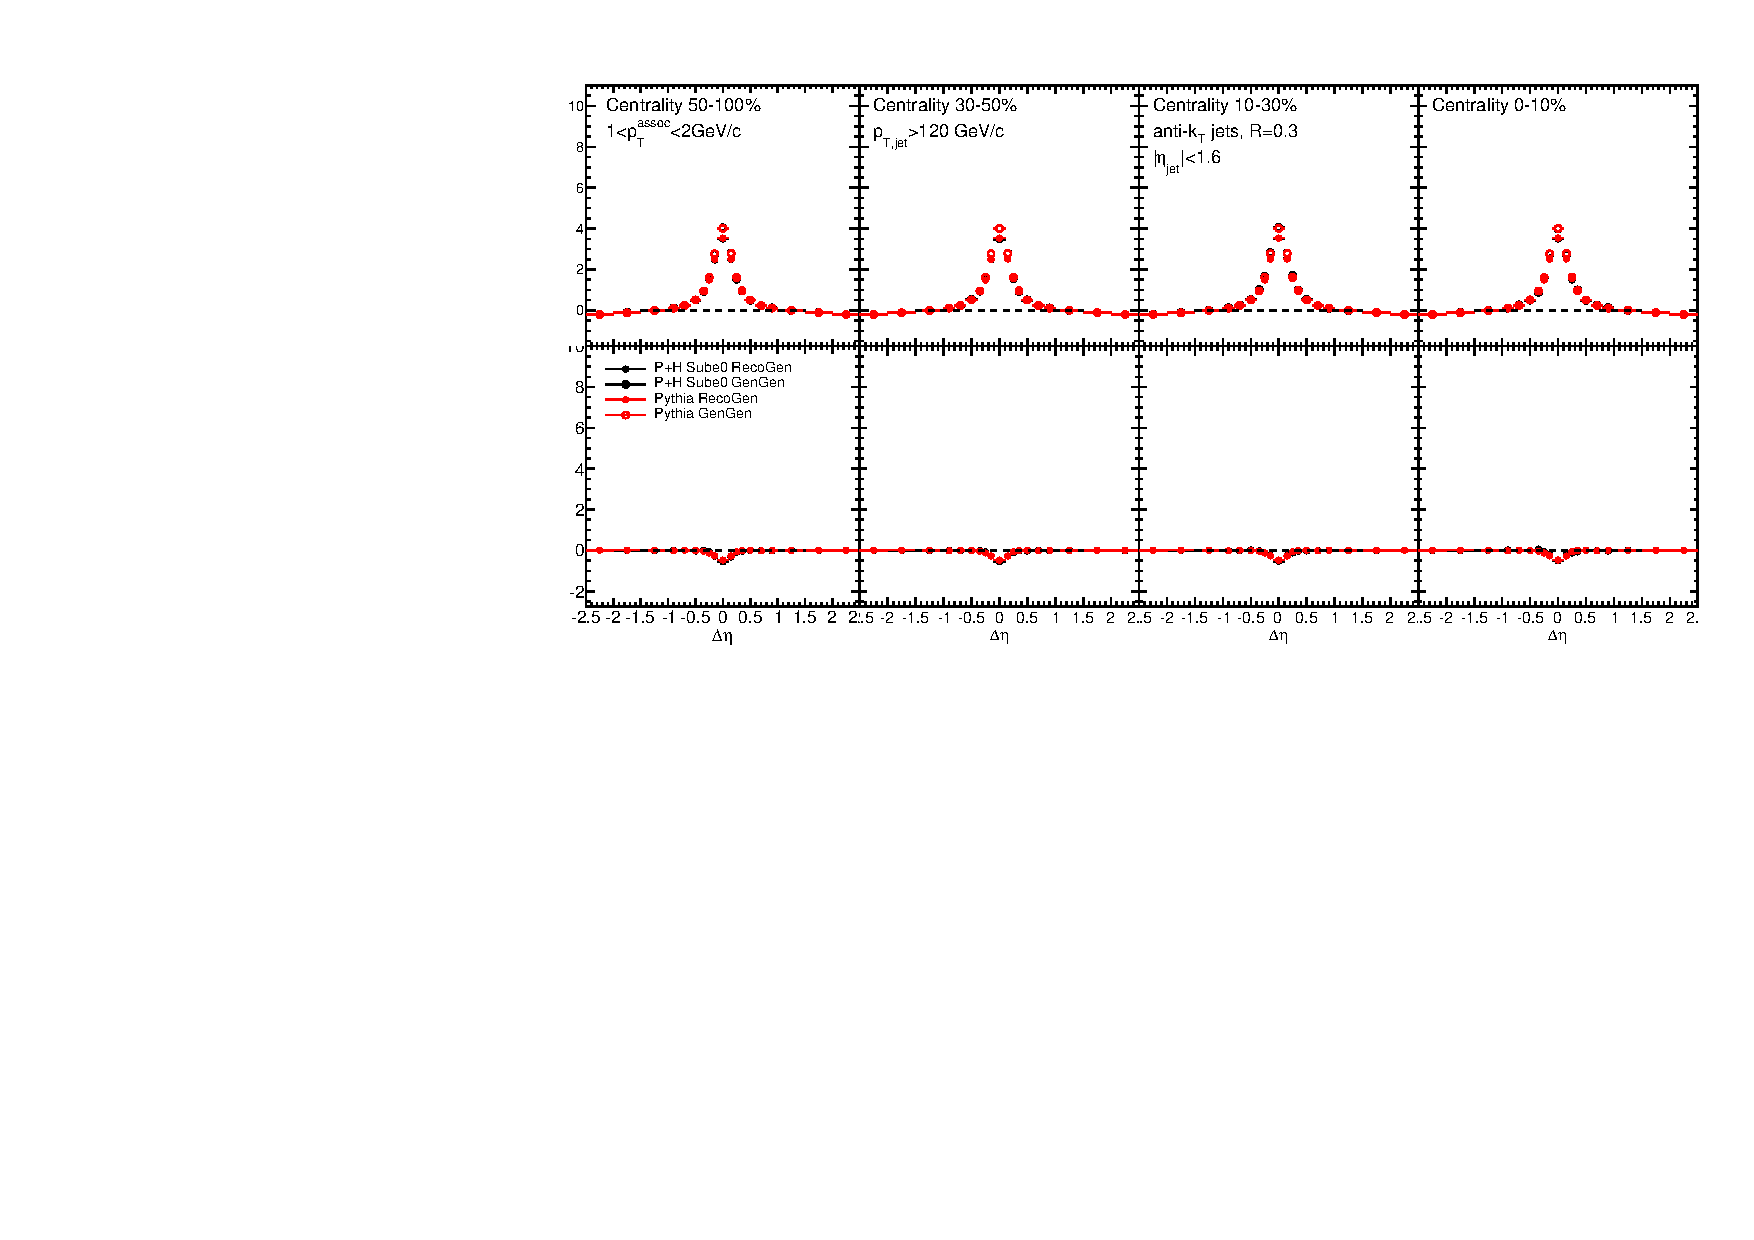
\includegraphics[width=0.99\textwidth]{figures/JFF_SpillOver/JFF_Residual_Corrections_Eta_Inclusive_TrkPt1_TrkPt2.pdf}
          \caption[Jet fragmentation function bias corrections for particles with $1<p_{\rm T}^{\rm trk}<2$ GeV]{$\Delta\eta$ jet fragmentation function bias corrections derived by comparing correlations between reconstructed vs. generated jets and generated {\sc pythia} events, with and without embedding into the {\sc hydjet} heavy ion environment, for particles $1<p_{\rm T}^{\rm trk}<2$ GeV.}
            \label{fig:jff_residual_inclusive_trkpt1_trkpt2}
            \end{center}
            \end{figure}
            
                      \begin{figure}[hbtp]
          \begin{center}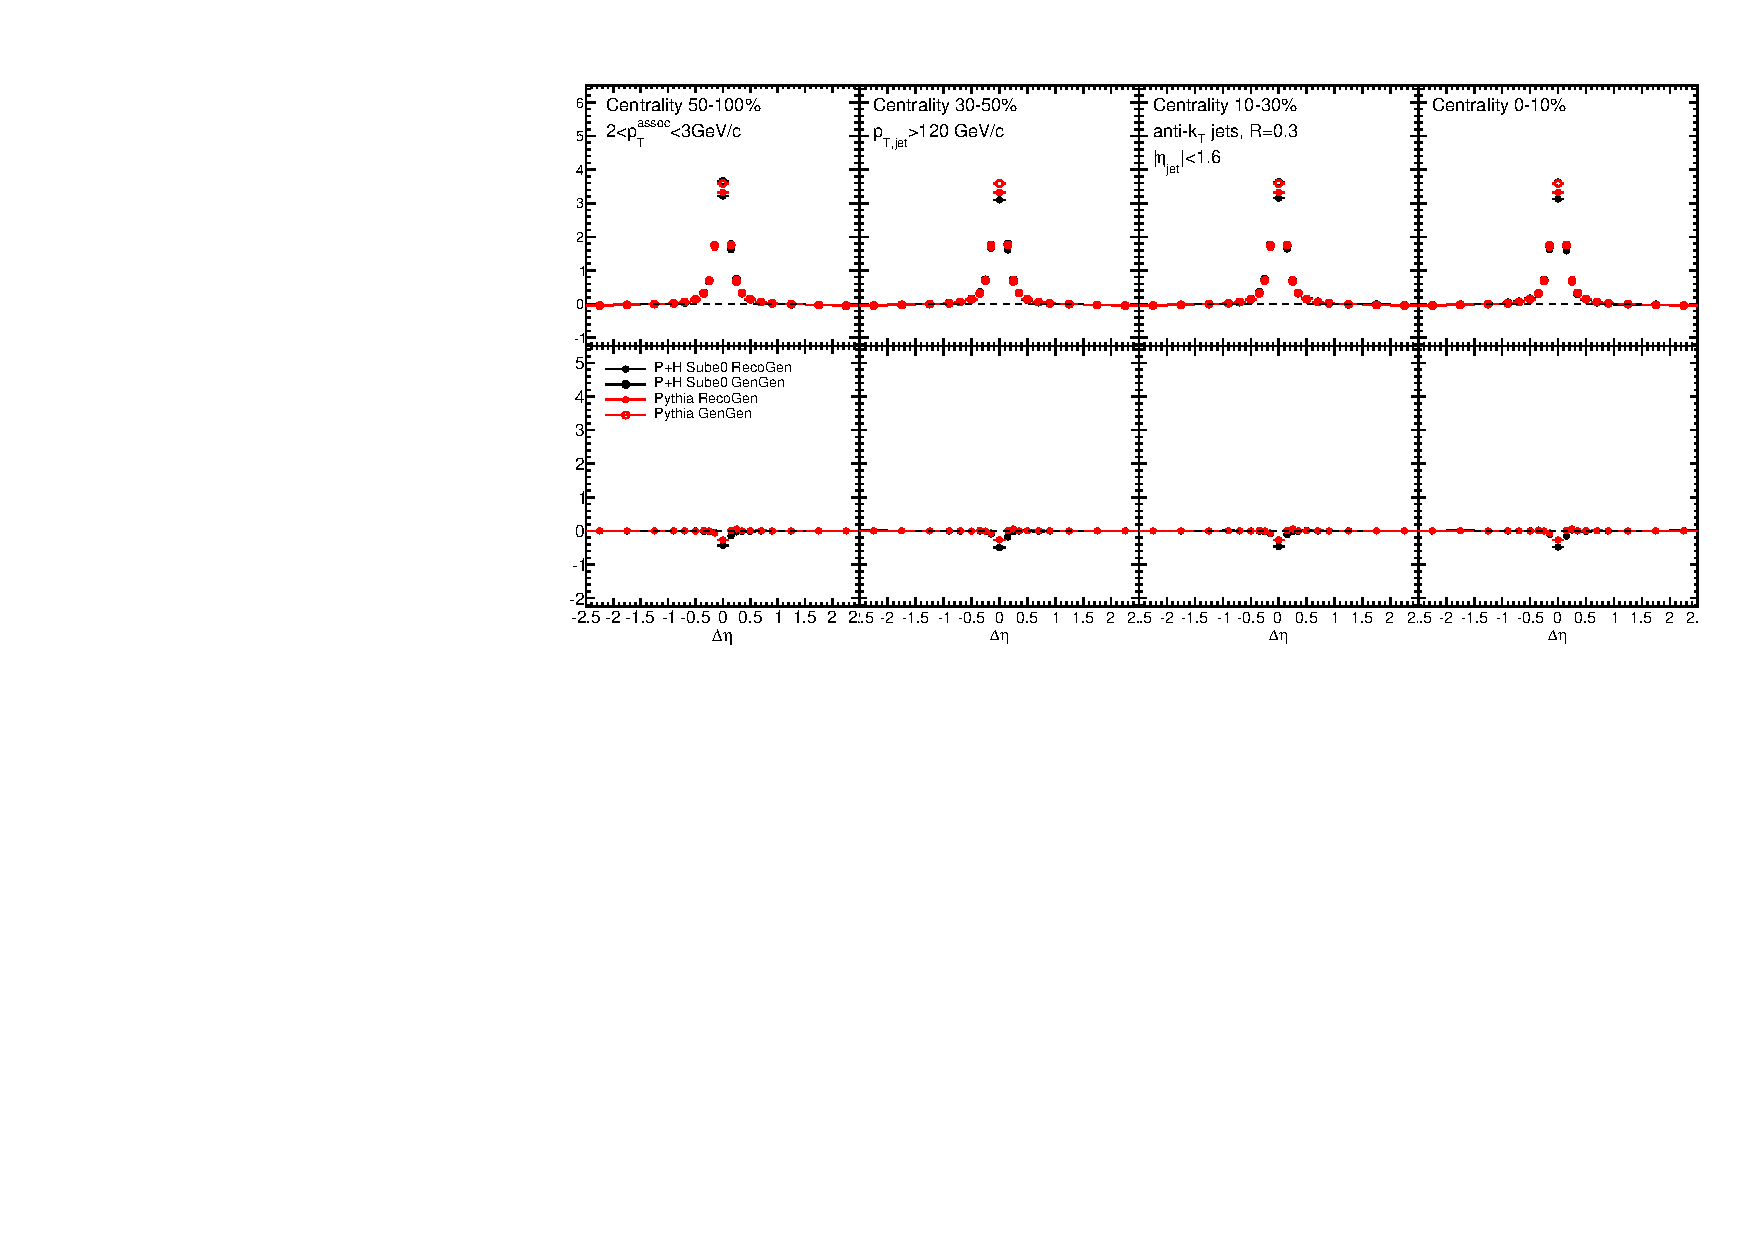
\includegraphics[width=0.99\textwidth]{figures/JFF_SpillOver/JFF_Residual_Corrections_Eta_Inclusive_TrkPt2_TrkPt3.pdf}
          \caption[Jet fragmentation function bias corrections for particles with $2<p_{\rm T}^{\rm trk}<3$ GeV]{$\Delta\eta$ jet fragmentation function bias corrections derived by comparing correlations between reconstructed vs. generated jets and generated {\sc pythia} events, with and without embedding into the {\sc hydjet} heavy ion environment, for particles $2<p_{\rm T}^{\rm trk}<3$ GeV.}
            \label{fig:jff_residual_inclusive_trkpt2_trkpt3}
            \end{center}
            \end{figure}
            
                      \begin{figure}[hbtp]
          \begin{center}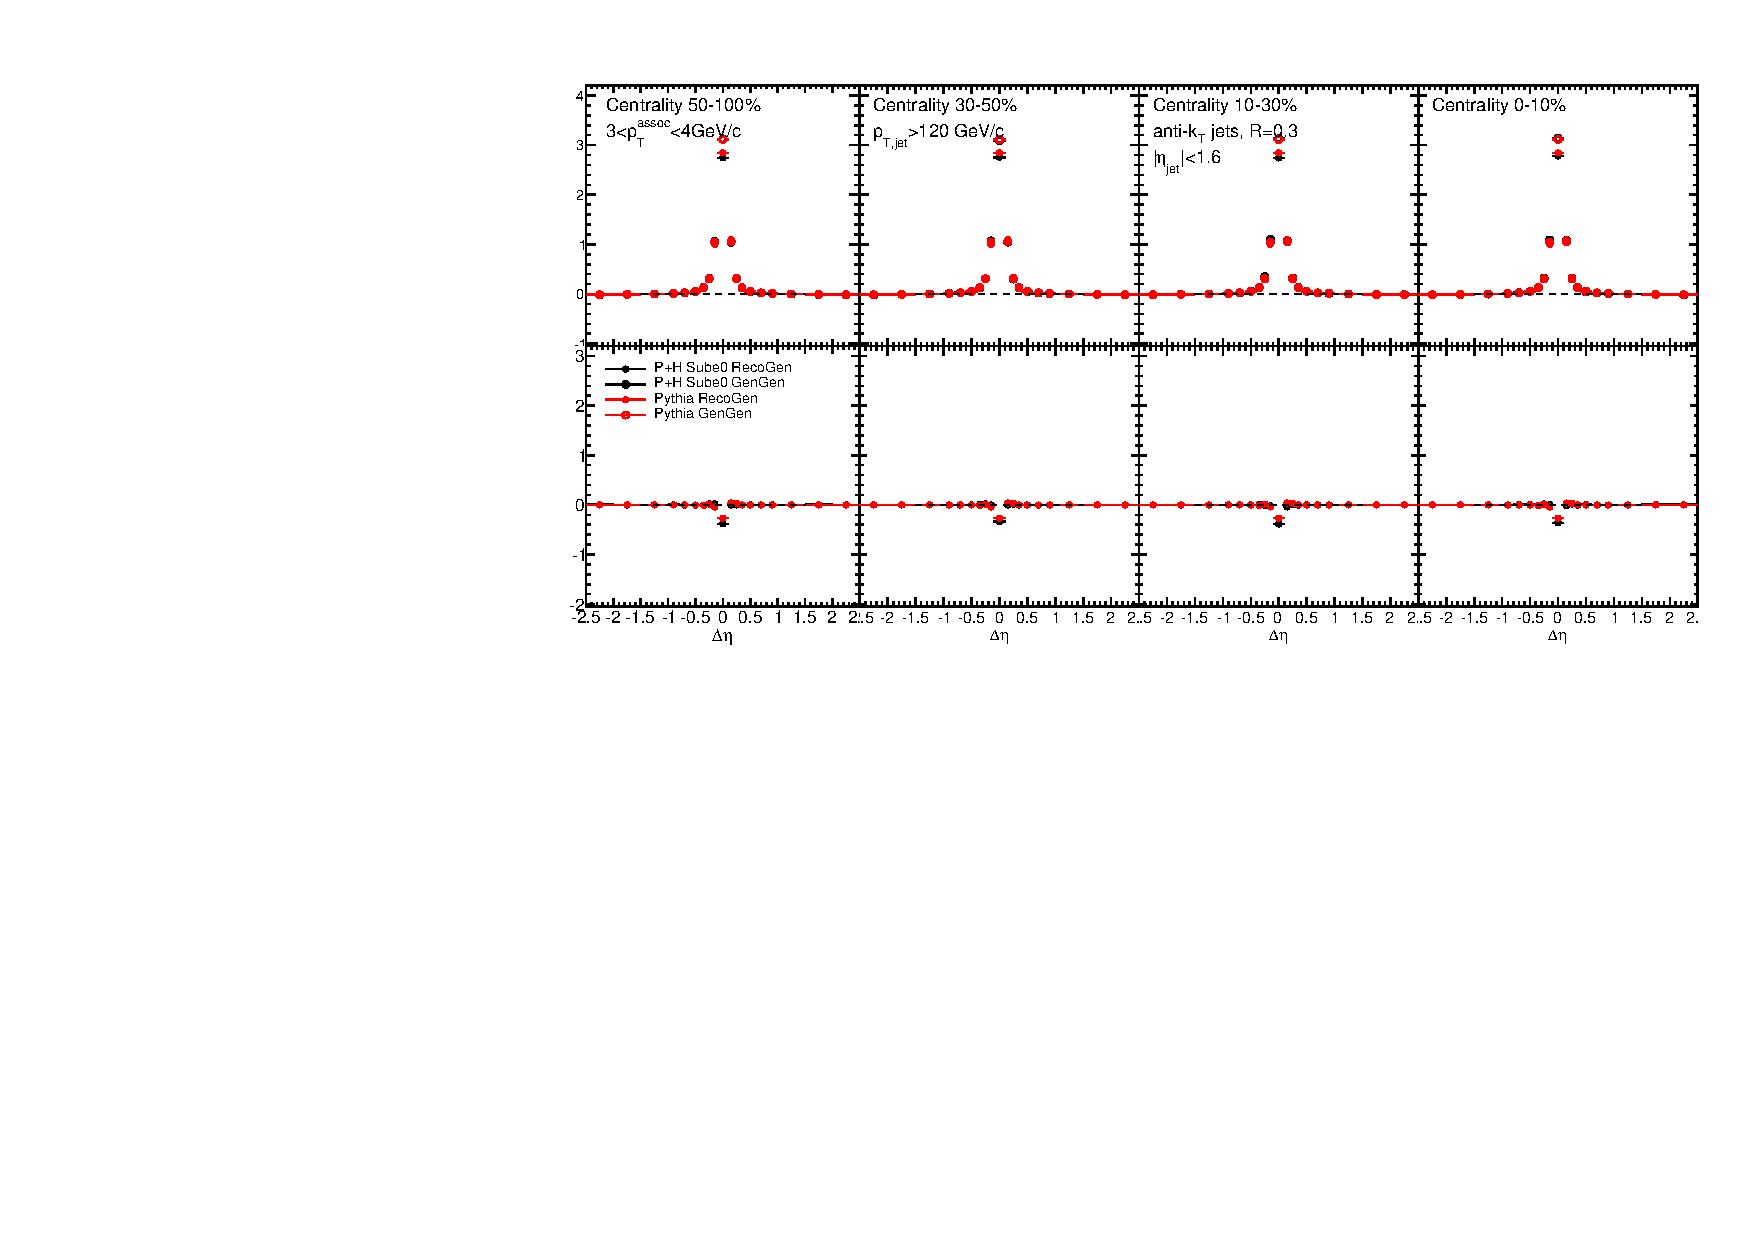
\includegraphics[width=0.99\textwidth]{figures/JFF_SpillOver/JFF_Residual_Corrections_Eta_Inclusive_TrkPt3_TrkPt4.pdf}
          \caption[Jet fragmentation function bias corrections for particles with $3<p_{\rm T}^{\rm trk}<4$ GeV]{$\Delta\eta$ jet fragmentation function bias corrections derived by comparing correlations between reconstructed vs. generated jets and generated {\sc pythia} events, with and without embedding into the {\sc hydjet} heavy ion environment, for particles $3<p_{\rm T}^{\rm trk}<4$ GeV.}
            \label{fig:jff_residual_inclusive_trkpt3_trkpt4}
            \end{center}
            \end{figure}
            
                      \begin{figure}[hbtp]
          \begin{center}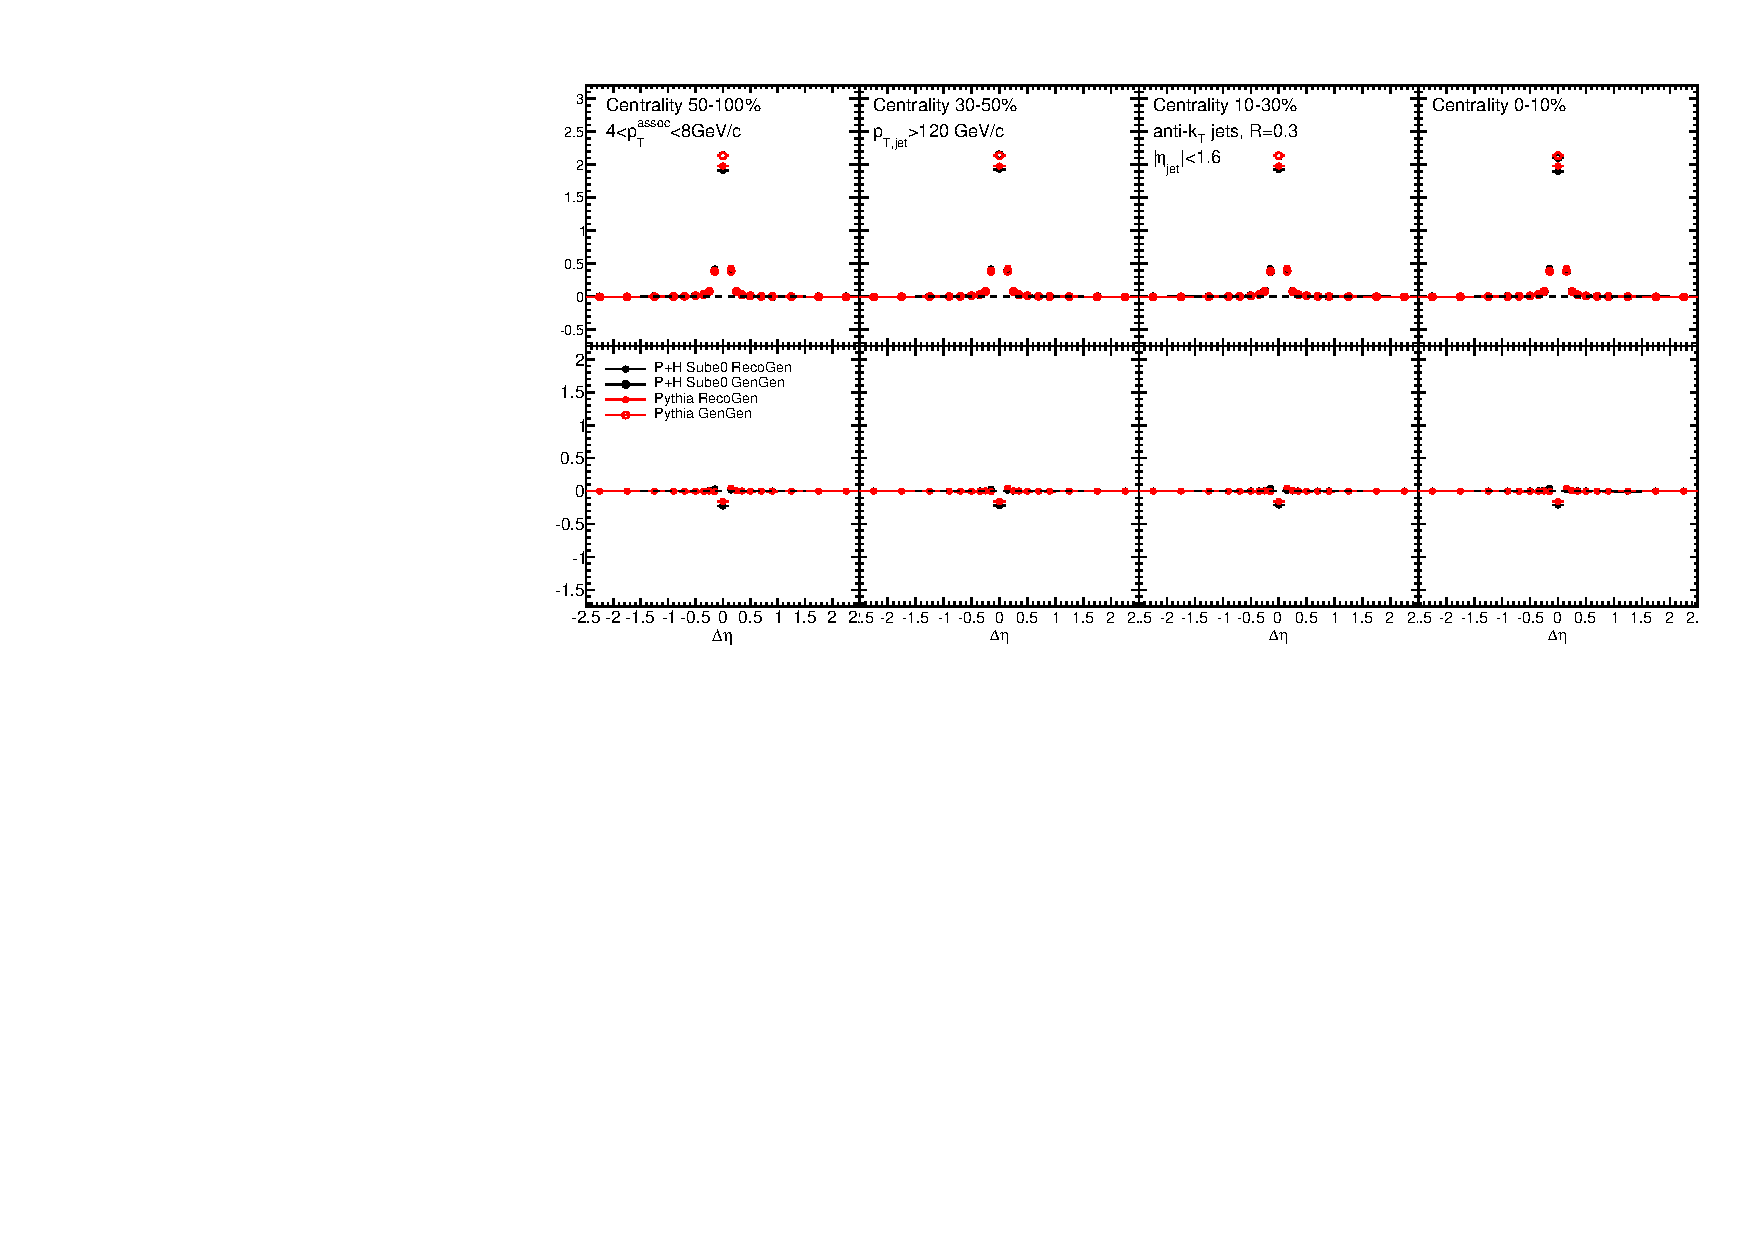
\includegraphics[width=0.99\textwidth]{figures/JFF_SpillOver/JFF_Residual_Corrections_Eta_Inclusive_TrkPt4_TrkPt8.pdf}
          \caption[Jet fragmentation function bias corrections for particles with $4<p_{\rm T}^{\rm trk}<8$ GeV]{$\Delta\eta$ jet fragmentation function bias corrections derived by comparing correlations between reconstructed vs. generated jets and generated {\sc pythia} events, with and without embedding into the {\sc hydjet} heavy ion environment, for particles $4<p_{\rm T}^{\rm trk}<8$ GeV.}
            \label{fig:jff_residual_inclusive_trkpt4_trkpt8}
            \end{center}
            \end{figure}
            
           \clearpage  
           
To assess the overall effect of these corrections, the integrated yield of these corrections is shown as a function of transverse momentum and centrality is shown for inclusive, leading, and subleading jets as a function of $p_{\rm T}^{\rm trk}$ in Fig.~\ref{fig:jff_residual_integrals_pT} and as a function of PbPb centrality in Fig.~\ref{fig:jff_residual_integrals_Cent}.  The correction magnitude shows little centrality dependence, and is very similar for pure {\sc pythia} simulation and {\sc pythia} embedded into {\sc hydjet}.  
            
                  \begin{figure}[h!]
                  \begin{center}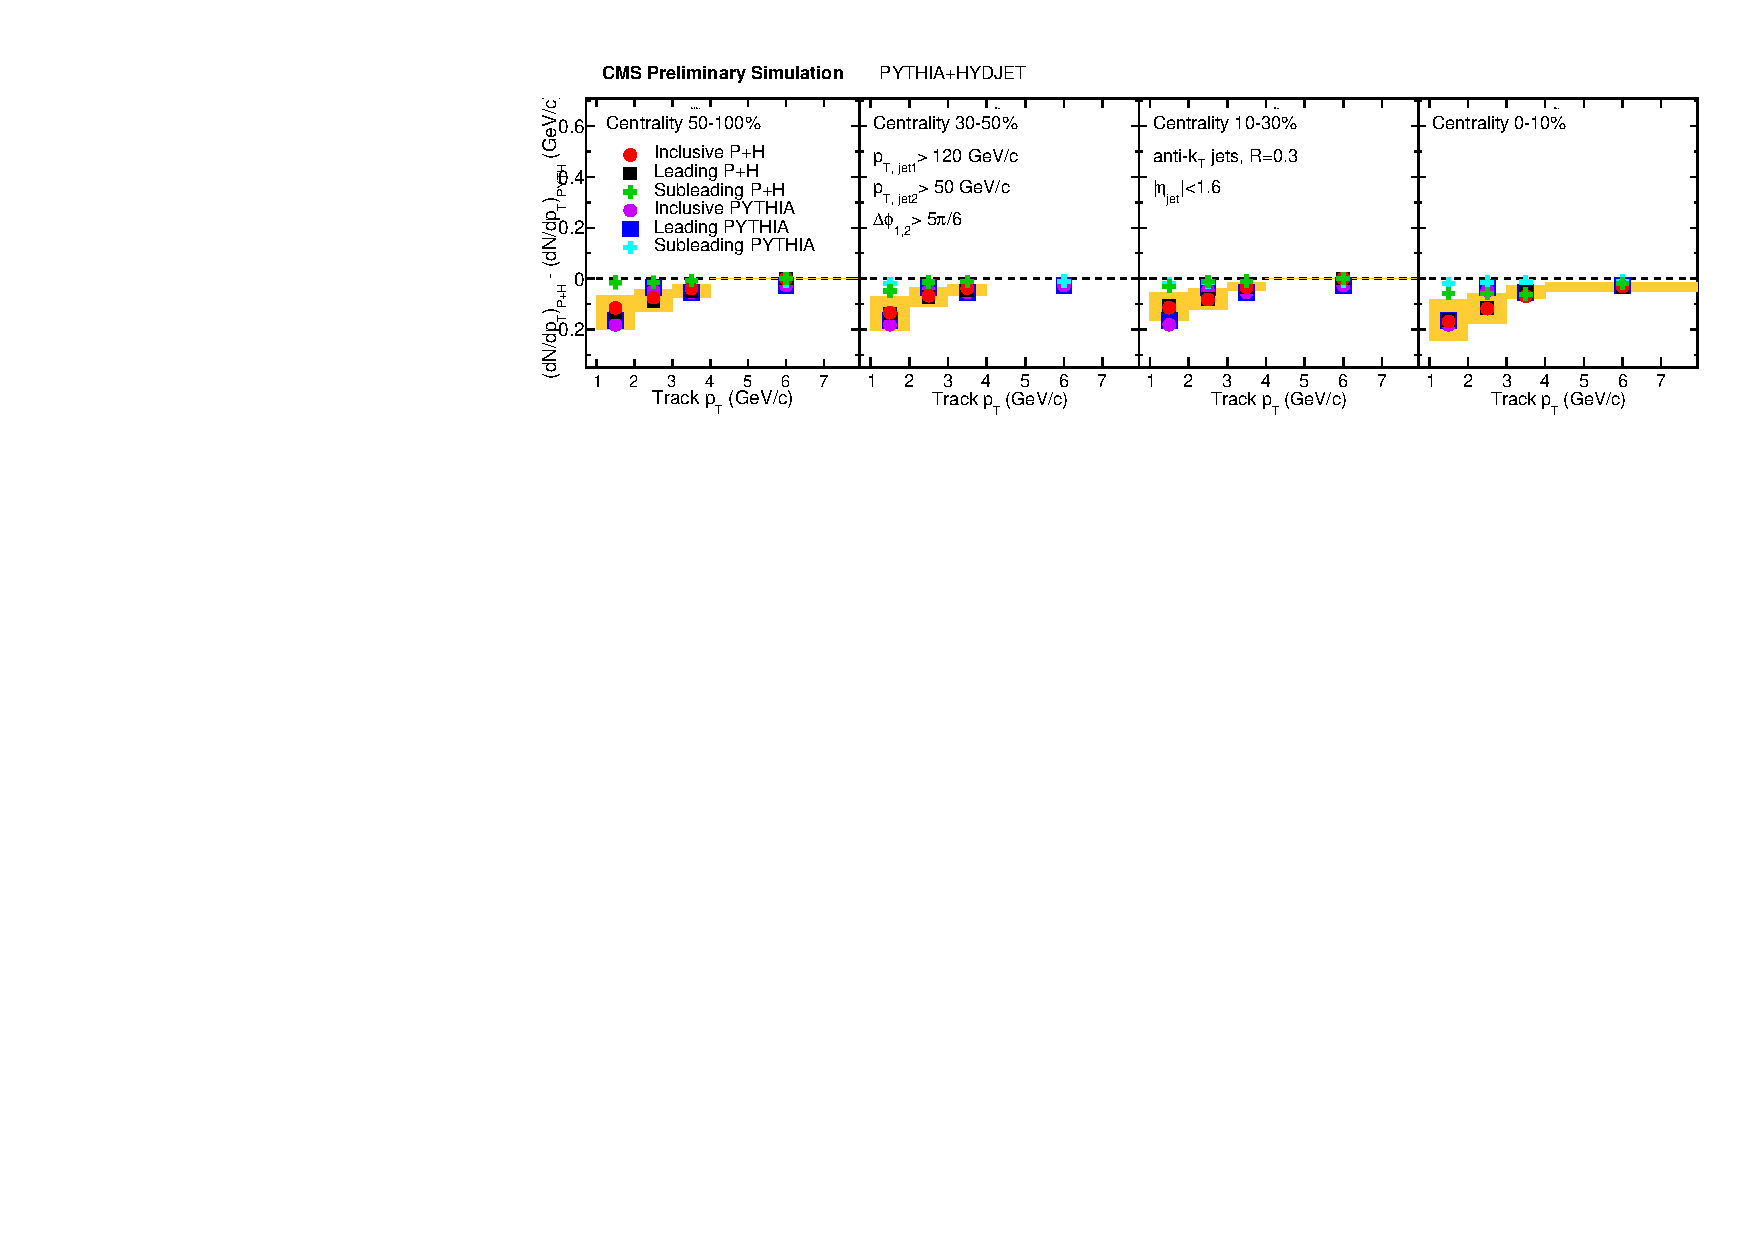
\includegraphics[width=0.99\textwidth]{figures/JFF_SpillOver/Integral_JFFResidual_pT.pdf}
                  \caption[Integrated yield attributed to jet fragmentation function bias as a function of $p_{\rm T}^{\rm trk}$]{Integrated yield attributed to jet fragmentation function bias in jet reconstruction for {\sc pythia} alone and embedded into {\sc hydjet}, shown as a function of $p_{\rm T}^{\rm trk}$ for each centrality class.}
                    \label{fig:jff_residual_integrals_pT}
                    \end{center}
                    \end{figure}

           
                  \begin{figure}[h!]
                  \begin{center}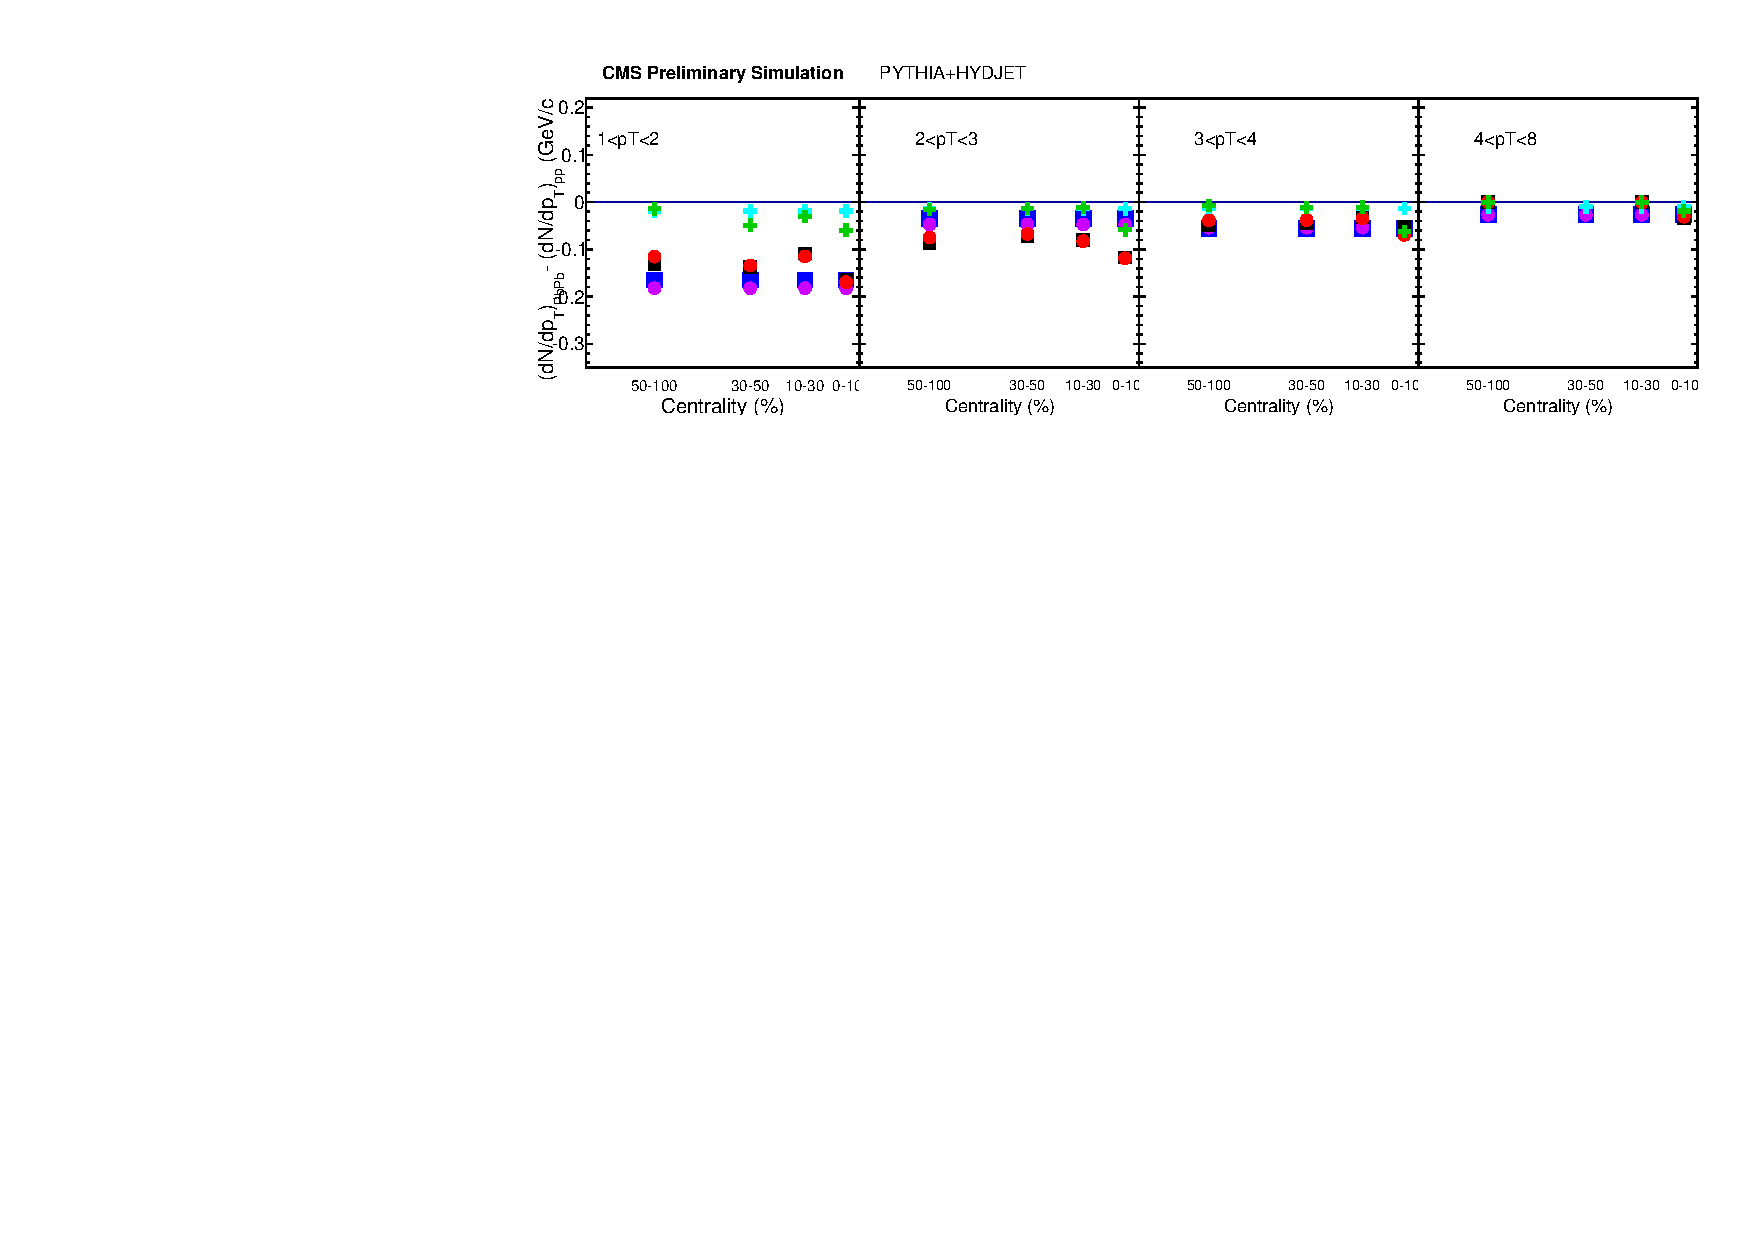
\includegraphics[width=0.99\textwidth]{figures/JFF_SpillOver/Integral_JFFResidual_Cent.pdf}
                  \caption[Integrated yield attributed to jet fragmentation function bias as a function of centrality]{Integrated yield attributed to jet fragmentation function bias in jet reconstruction for {\sc pythia} alone and embedded into {\sc hydjet}, shown as a function of centrality for each associate track $p_{\rm T}$ range.}
                    \label{fig:jff_residual_integrals_Cent}
                    \end{center}
                    \end{figure}
                    
\clearpage




\subsection{Background fluctuation bias correction}

In central PbPb collisions background levels are very high, and naturally fluctuate throughout the event.  As discussed in Section~\ref{sec:Jets}, the process of jet reconstruction in PbPb collisions includes background subtraction that accounts for the general distirbution of energy in the event.  However, small, local variations in background levels remain (on the order of 5 GeV within a radius of R = 0.3).  These are reconstructed into the jet, raising or lowering the measured jet energy depending on whether the jet sits on an upward or a downward fluctuation in the background.  As a result, jets with ``true'' $p_{\rm T}$ slightly below the 120 GeV selection threshold that sit on upward background fluctuations will be included in the sample, while jets sit on downward will be excluded.  Because the jet spectrum is steeply falling, it is much more common for a lower-$p_{\rm T}$ jet (on an upward fluctuation) to be included in the sample than for a higher-$p_{\rm T}$ jet to be excluded.  This results in the systematic inclusion of tracks from background fluctuations in the peak of tracks observed about the jet axis, resulting in a contribution to the initially measured jet peak that must be accurately quantified and subtracted.  

To estimate and subtract the contribution to the excess yield due to background fluctuation bias in jet reconstruction  to the measured excess yield, we perform simulations in {\sc pythia+hydjet} samples with reconstructed jets (but generated tracks, as the tracking efficiency uncertainty is analyzed separately), and construct correlations excluding particles generated with the embedded {\sc pythia} hard-scattering process.  As the {\sc pythia+hydjet} simulation does not include interactions between the {\sc pythia} hard process and the medium, this procedure by construction isolates the contribution to the jet peak that is attributable to the background fluctuation bias. The resulting corrections are illustrated in Fig.~\ref{fig:reco_reco_closure_deta_inc} -  Fig.~\ref{fig:reco_reco_closure_inc4} for inclusive jets at 2.76 TeV.  These correlations show a diminishing effect with increasing particle transverse momentum.  We subtract the gaussian fit to these correlations bin-by-bin from the data results, and also assign the half its magnitude as systematic uncertainty to the final measurements.  To assess the overall effect of these corrections, the integrated yield of these corrections is shown in Fig.~\ref{fig:closure_integrals_pT} as a function of transverse momentum and centrality is shown for inclusive, leading, and subleading jets at 2.76 TeV. 


      \begin{figure}[hbtp]
      \begin{center}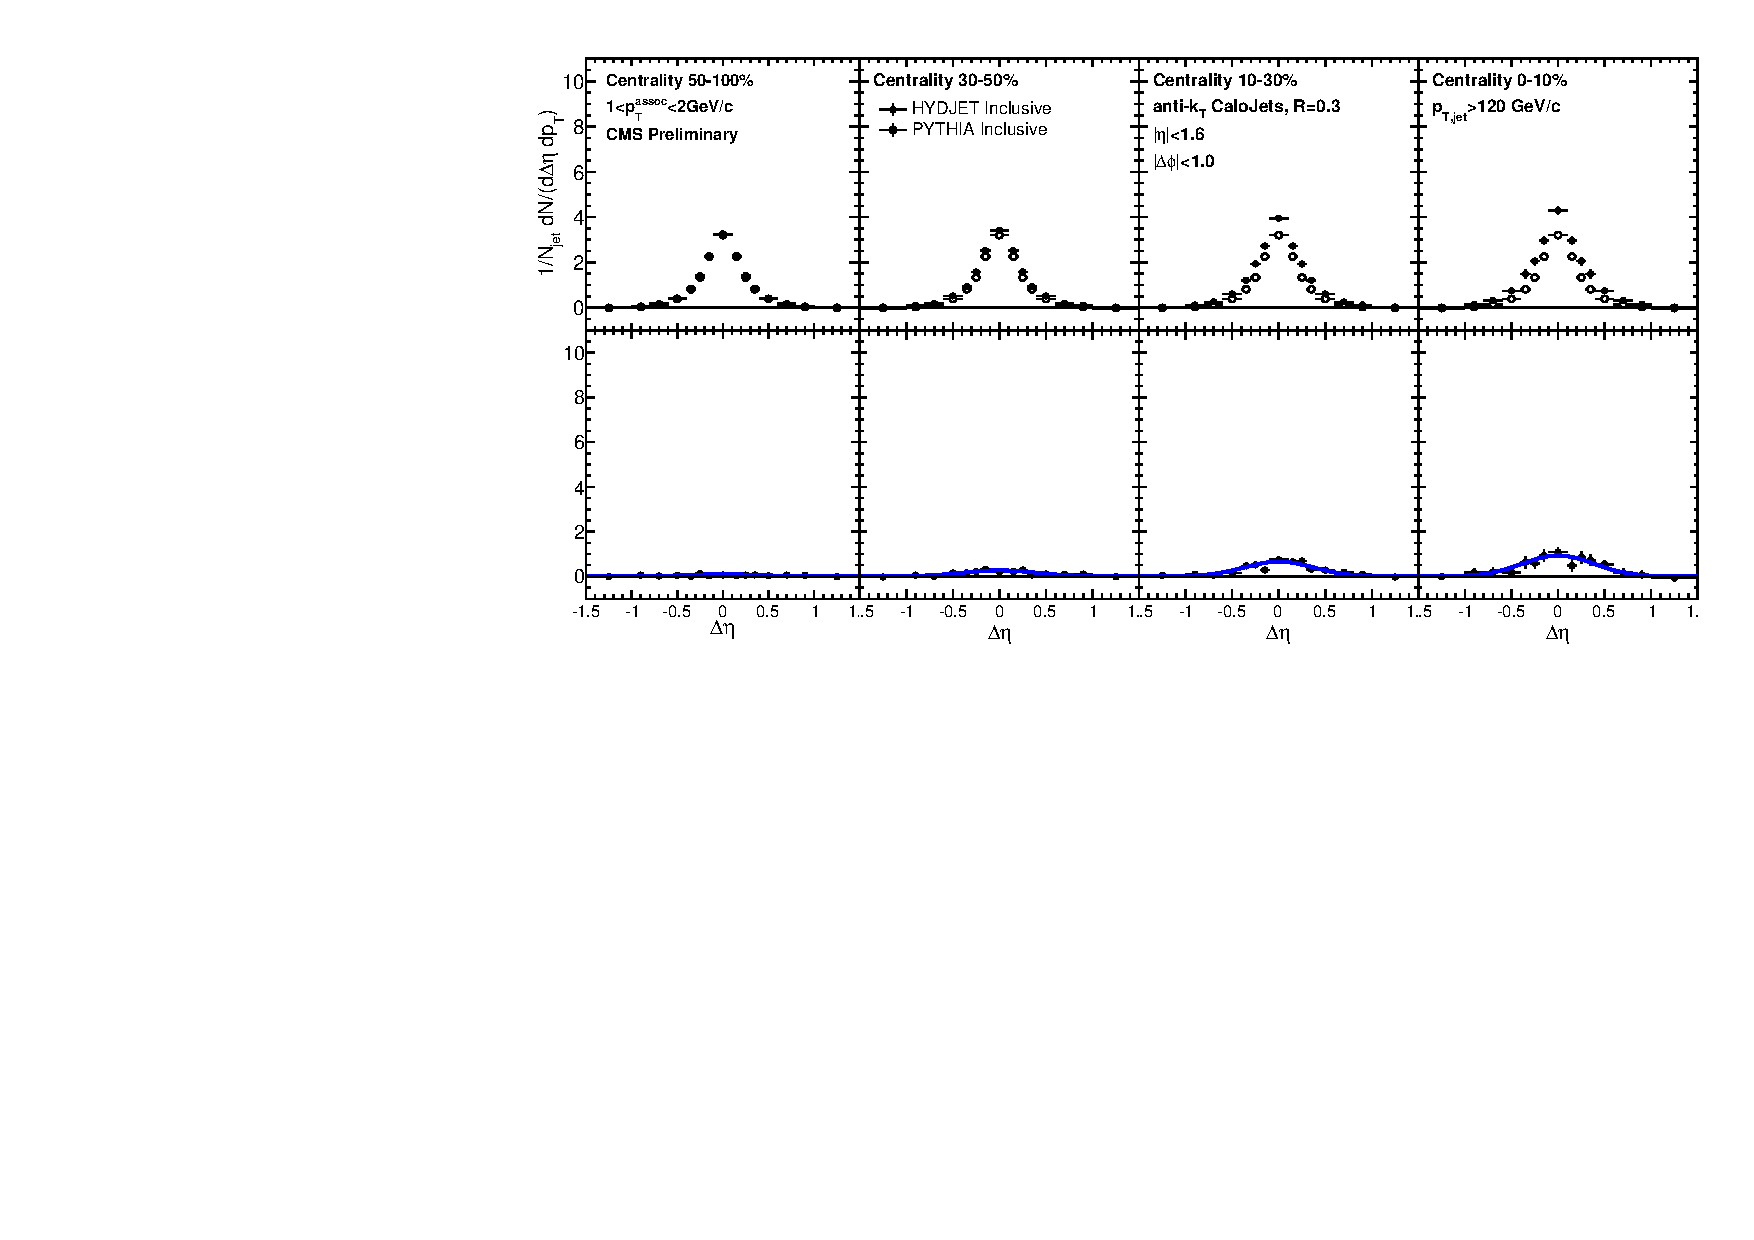
\includegraphics[width=0.99\textwidth]{figures/JFF_SpillOver/AN_Closures_Eta_InclusiveTrkPt1_TrkPt2.pdf}
      \caption[Background fluctuation bias corrections for particles with $1<p_{\rm T}^{\rm trk}<2$ GeV]{$\Delta\eta$ background fluctuation bias correction for inclusive jets derived by constructing correlations in {\sc pythia+hydjet} between reconstructed jets and only those tracks simulated as part of the heavy ion underlying event rather than the embedded {\sc pythia} hard process, for particles $1<p_{\rm T}^{\rm trk}<2$ GeV}
        \label{fig:reco_reco_closure_deta_inc}
        \end{center}
        \end{figure}



   \begin{figure}[hbtp]
              \begin{center}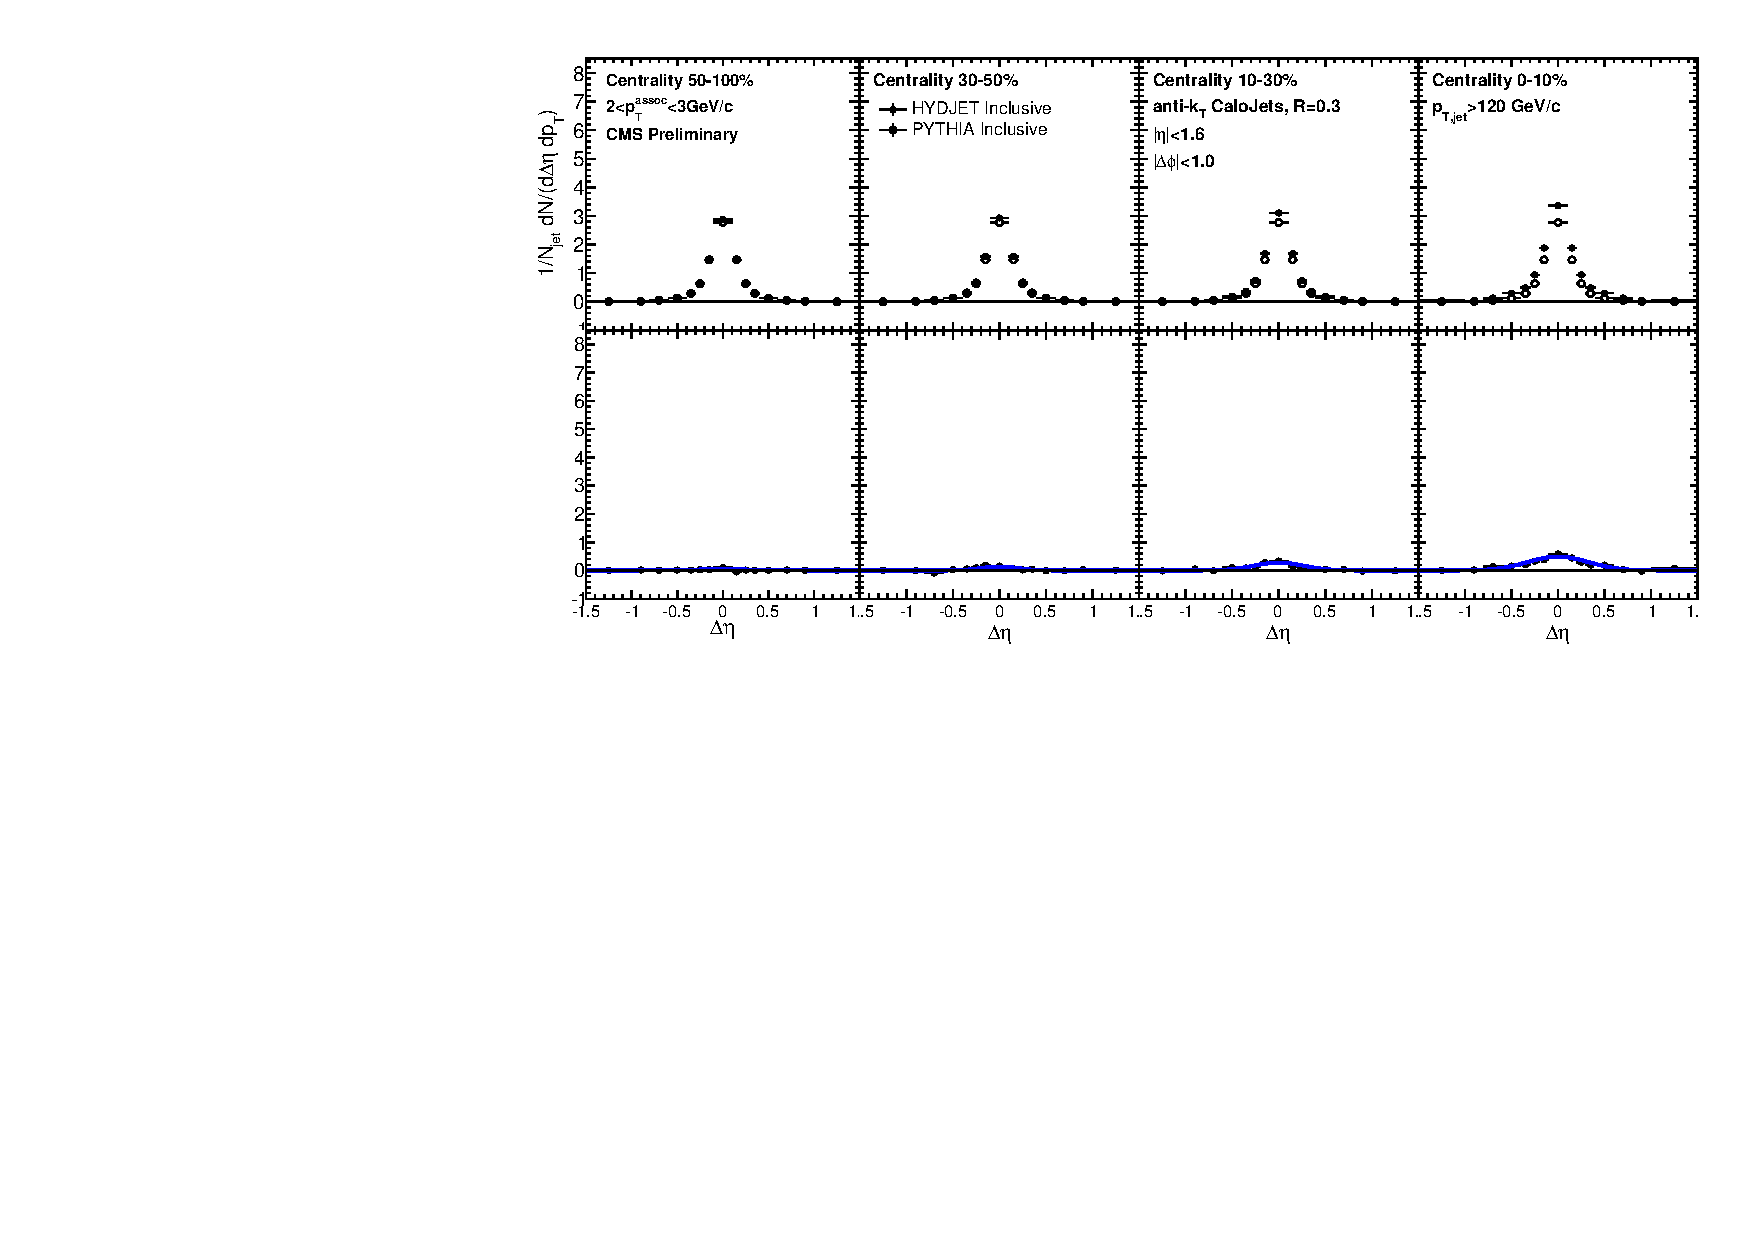
\includegraphics[width=0.99\textwidth]{figures/JFF_SpillOver/AN_Closures_Eta_InclusiveTrkPt2_TrkPt3.pdf}
             \caption[Background fluctuation bias corrections for particles with $2<p_{\rm T}^{\rm trk}<3$ GeV]{$\Delta\eta$ background fluctuation bias correction for inclusive jets derived by constructing correlations in {\sc pythia+hydjet} between reconstructed jets and only those tracks simulated as part of the heavy ion underlying event rather than the embedded {\sc pythia} hard process, for particles $2<p_{\rm T}^{\rm trk}<3$ GeV}
                \label{fig:reco_reco_closure_inc2}
                \end{center}
                \end{figure}

                \begin{figure}[hbtp] 
                \begin{center}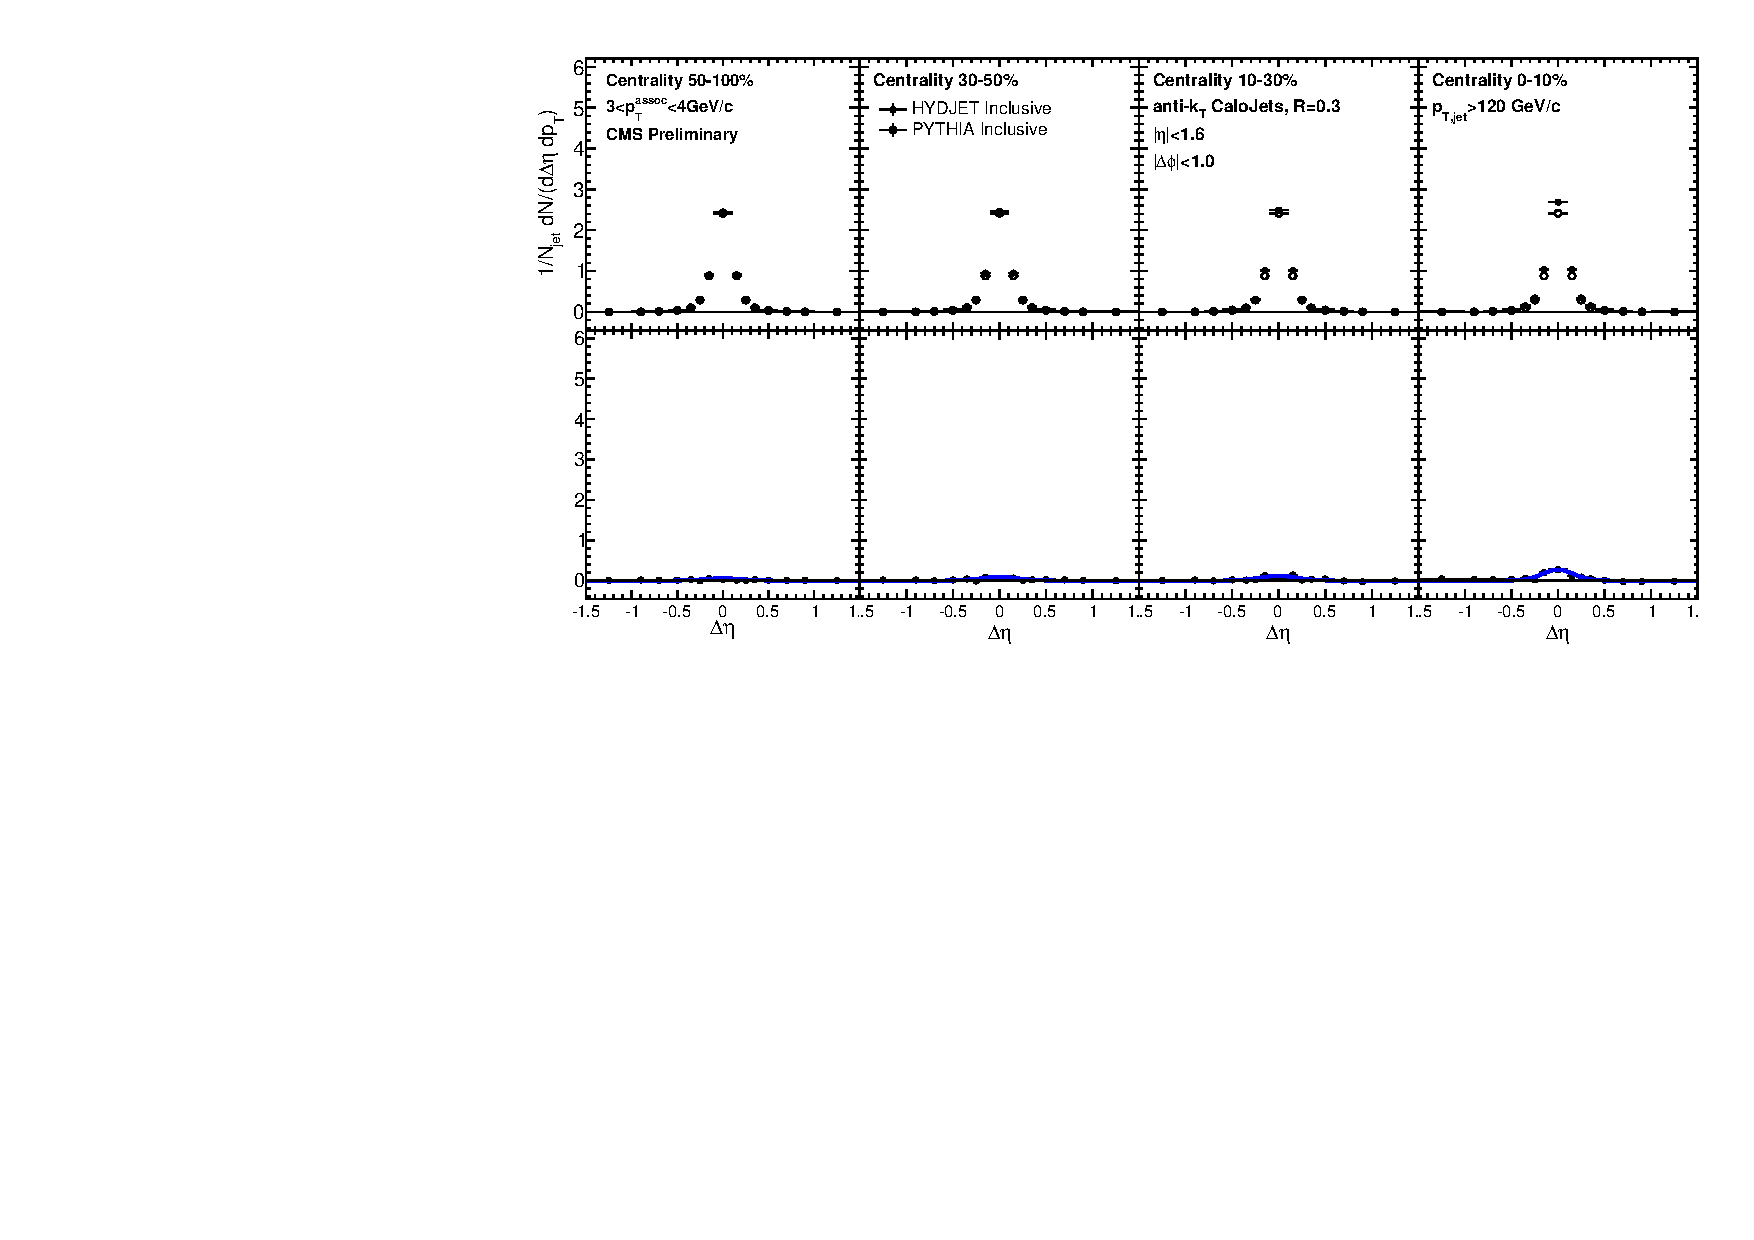
\includegraphics[width=0.99\textwidth]{figures/JFF_SpillOver/AN_Closures_Eta_InclusiveTrkPt3_TrkPt4.pdf}
               \caption[Background fluctuation bias corrections for particles with $3<p_{\rm T}^{\rm trk}<4$ GeV]{$\Delta\eta$ background fluctuation bias correction for inclusive jets derived by constructing correlations in {\sc pythia+hydjet} between reconstructed jets and only those tracks simulated as part of the heavy ion underlying event rather than the embedded {\sc pythia} hard process, for particles $3<p_{\rm T}^{\rm trk}<4$ GeV}

                  \label{fig:reco_reco_closure_inc3}
                  \end{center}
                  \end{figure}


                  \begin{figure}[hbtp]
                  \begin{center}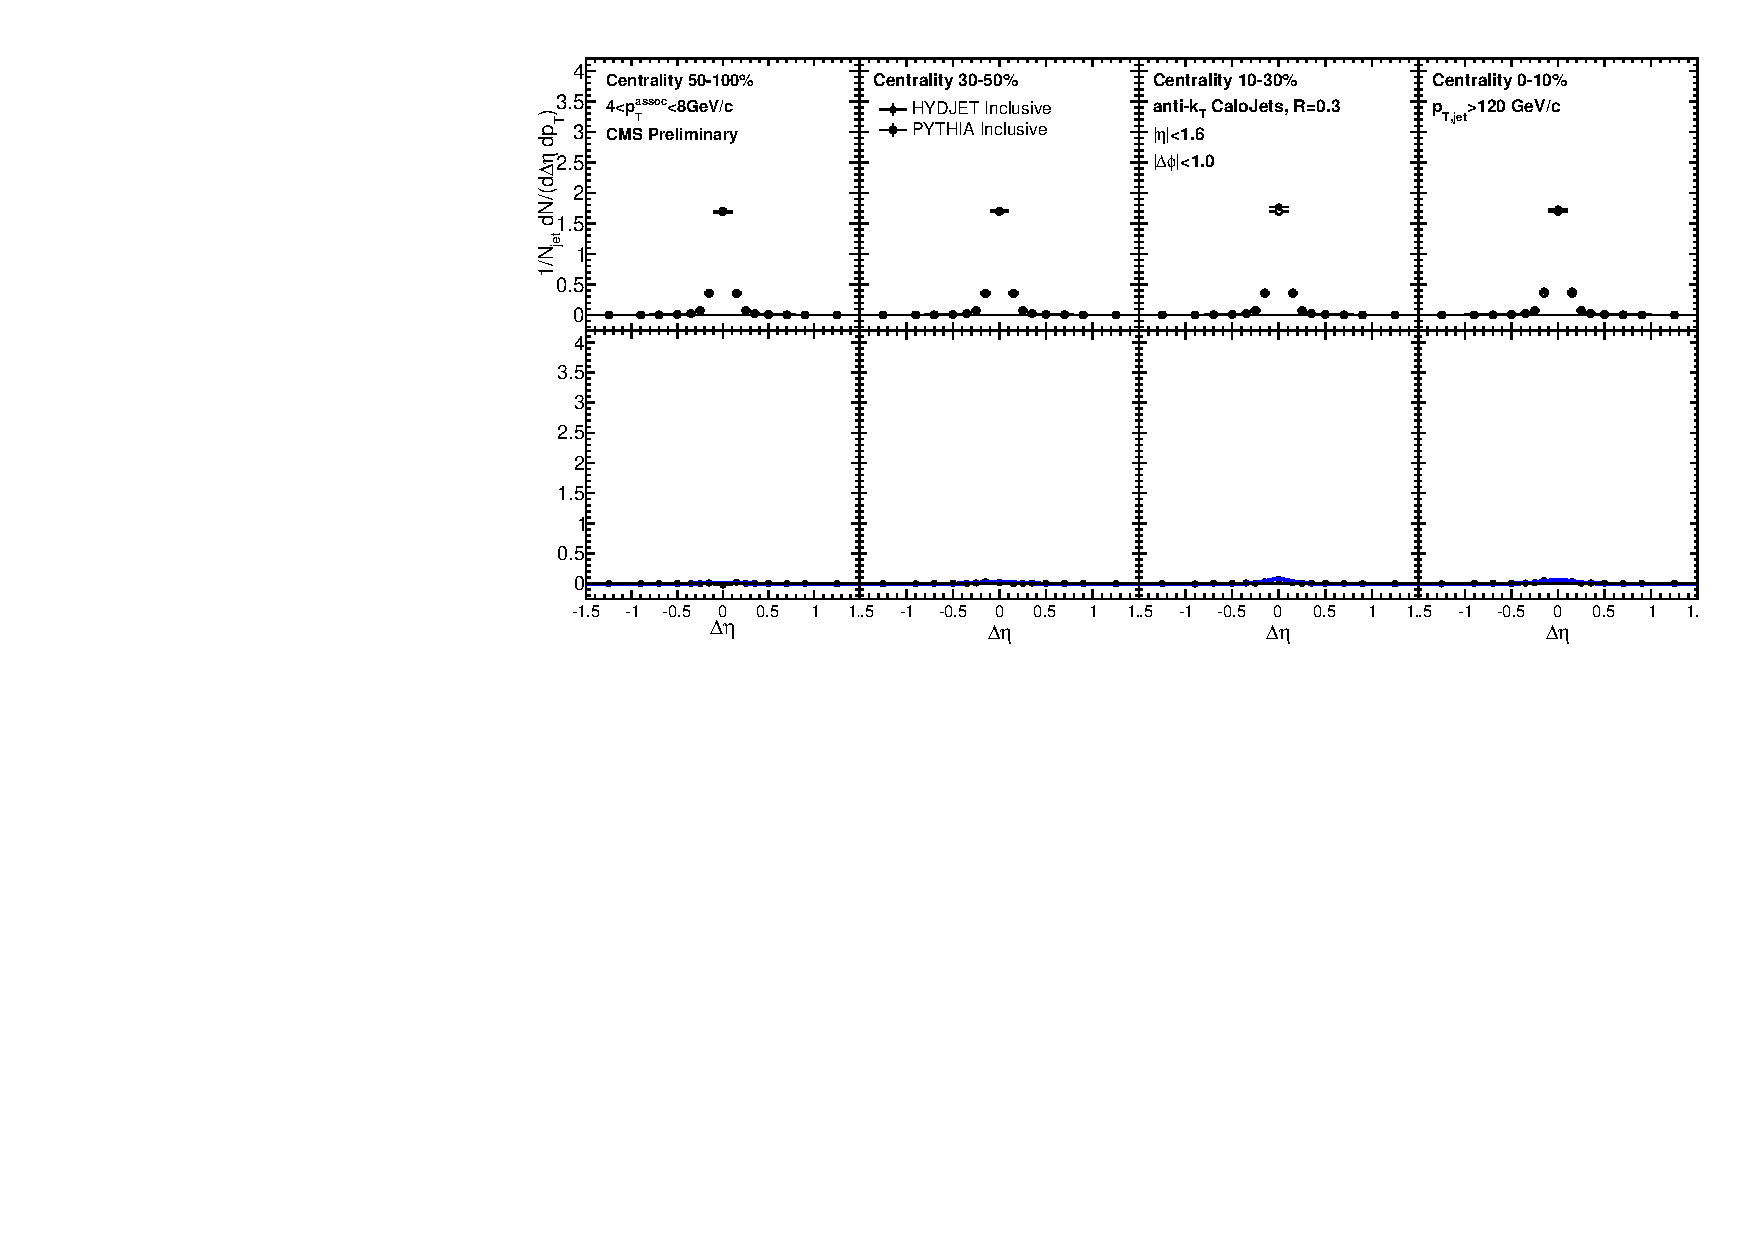
\includegraphics[width=0.99\textwidth]{figures/JFF_SpillOver/AN_Closures_Eta_InclusiveTrkPt4_TrkPt8.pdf}
                 \caption[Background fluctuation bias corrections for particles with $4<p_{\rm T}^{\rm trk}<8$ GeV]{$\Delta\eta$ background fluctuation bias correction for inclusive jets derived by constructing correlations in {\sc pythia+hydjet} between reconstructed jets and only those tracks simulated as part of the heavy ion underlying event rather than the embedded {\sc pythia} hard process, for particles $4<p_{\rm T}^{\rm trk}<8$ GeV}
                    \label{fig:reco_reco_closure_inc4}
                    \end{center}
                    \end{figure}

       
                  \begin{figure}[h!]
                  \begin{center}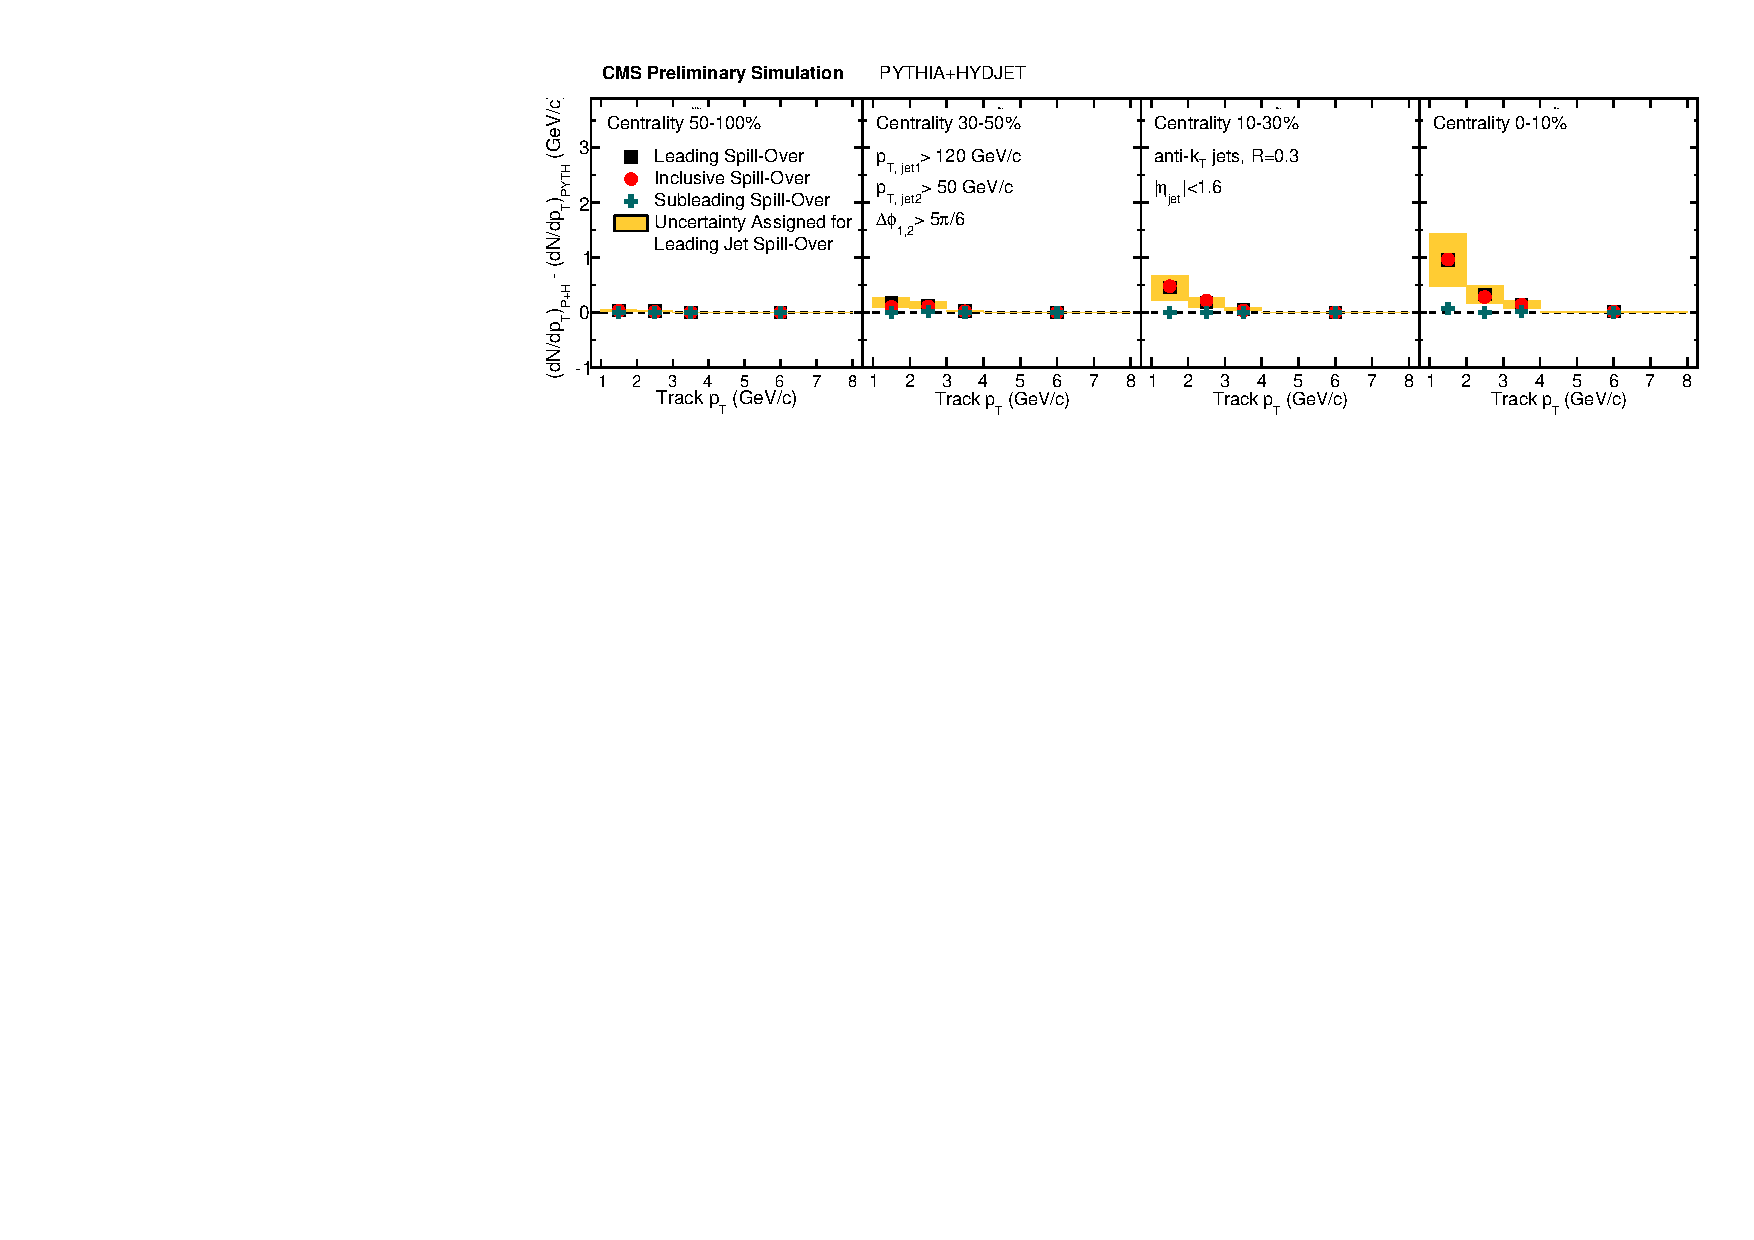
\includegraphics[width=0.99\textwidth]{figures/JFF_SpillOver/Integral_Closure_pT_Leading.pdf}
                  \caption[Integrated yield attributed to background fluctuation bias as a function of $p_{\rm T}^{\rm trk}$]{Integrated yield attributed to background fluctuation bias in the selection of inclusive and leading jets, shown as a function of associate track $p_{\rm T}$ for each centrality class.}
                    \label{fig:closure_integrals_pT}
                    \end{center}
                    \end{figure}
                    

Considering that the background fluctuation bias effect in many ways mimics the jet peak signal, it is particularly important to validate this correction and confirm both that its origin is well-understood and that the {\sc hydjet} simulation used to derive it reproduces the background fluctuations in data closely enough to accurately obtain corrections.  To check this, we extract a direct estimate of the effect from data using a ``pseudo-embedding'' of pp jets into a minimum bias PbPb data sample.  The goal of this study is to verify that we recover a similar magnitude of excess yield as we attribute based on our more detailed {\sc pythia+hydjet} simulations.  Here we approximate the effect by adding the total transverse momentum in a circle of radius  $R = 0.3$ around all jets with $p_{\rm T} > 90$ GeV, and considering the total deviation up or down of this $(\Sigma p_{\rm T})_{\rm cone}$ from the average total transverse momentum $< (\Sigma p_{\rm T})_{\rm cone}>$.  First, we may directly compare the average $p_{\rm T}$ and fluctuations in $p_{\rm T}$ in these random cones between data and Monte Carlo.  We find that our Monte Carlo approximately reproduces the data:  in data $< (\Sigma p_{\rm T})_{\rm cone, data}> = 10.0$ GeV, with $\sigma((\Sigma p_{\rm T})_{\rm cone, data}) = 4.9$ GeV, while in Monte Carlo $< (\Sigma p_{\rm T})_{\rm cone, MC}> = 11.9$ GeV, with $\sigma((\Sigma p_{\rm T})_{\rm cone, data}) = 5.6$ GeV. 

We then use these random cones to adjust jet energy and re-select jets:  we add the deviation up or down of this $(\Sigma p_{\rm T})_{\rm cone}$ to each embedded pp jets with this adjusted $p_{\rm T}$.  We then fill $\Delta\eta - \Delta\phi$ correlations to all jets that pass our nominal $p_{\rm T} > 120$ GeV jet selection cut.  We apply this technique to both our {\sc pythia+hydjet} sample and a minimum-bias PbPb data sample to measure the charged particle yield associated with the embedded jet axis as a result of the jet fluctuation bias.  As Fig.~\ref{fig:data_spill_int}--\ref{fig:data_spill_bins} show, this data pseudo-embedding recovers the same magnitude of excess yield due to background fluctuation bias as our nominal Monte Carlo studies, but artificially confines this effect to a $R = 0.3$ cone by construction, due to the artificially simple jet reconstruction procedure.  This gives confidence that the origin and magnitude of the effect are well-understood.

\begin{figure}[h!]
\begin{center}
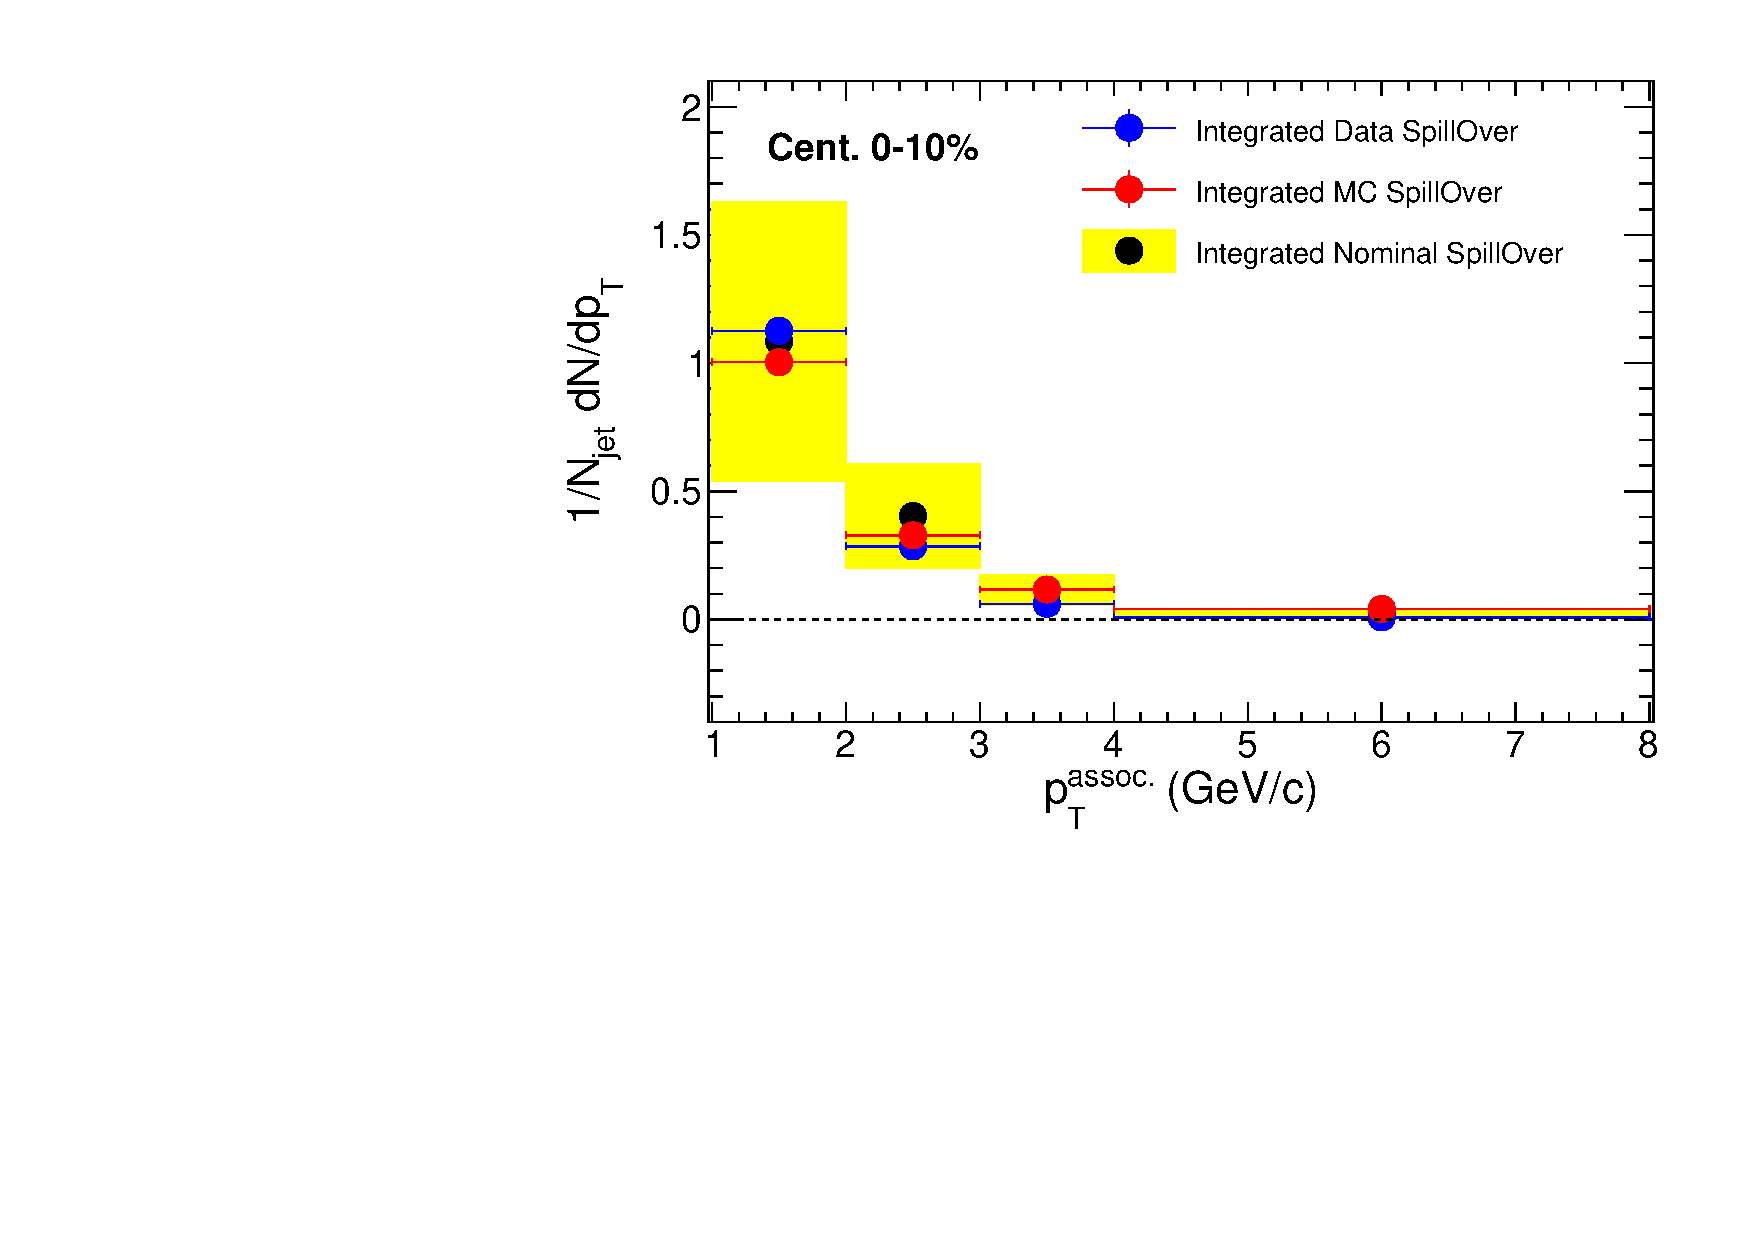
\includegraphics[width=0.49\textwidth]{figures/JFF_SpillOver/Data_Closure_Integrals.pdf}

\caption[Data-driven check of integrated yields attributed to background fluctuation bias]{Total integrated magnitude of background fluctuation bias as simulated with pp jets embedded in Minimum Bias events (blue points) compared to the effect as simulated with {\sc pythia}  jets into minimum bias {\sc hydjet} and to nominal corrections obtained with full {\sc pythia+hydjet} simulation. Nominal systematic errors of +/- 50\% as assigned in this analysis are shown as yellow systematic error bars on nominal (full MC simulation) points.}
\label{fig:data_spill_int}
\end{center}
\end{figure}


\begin{figure}[h!]
\begin{center}
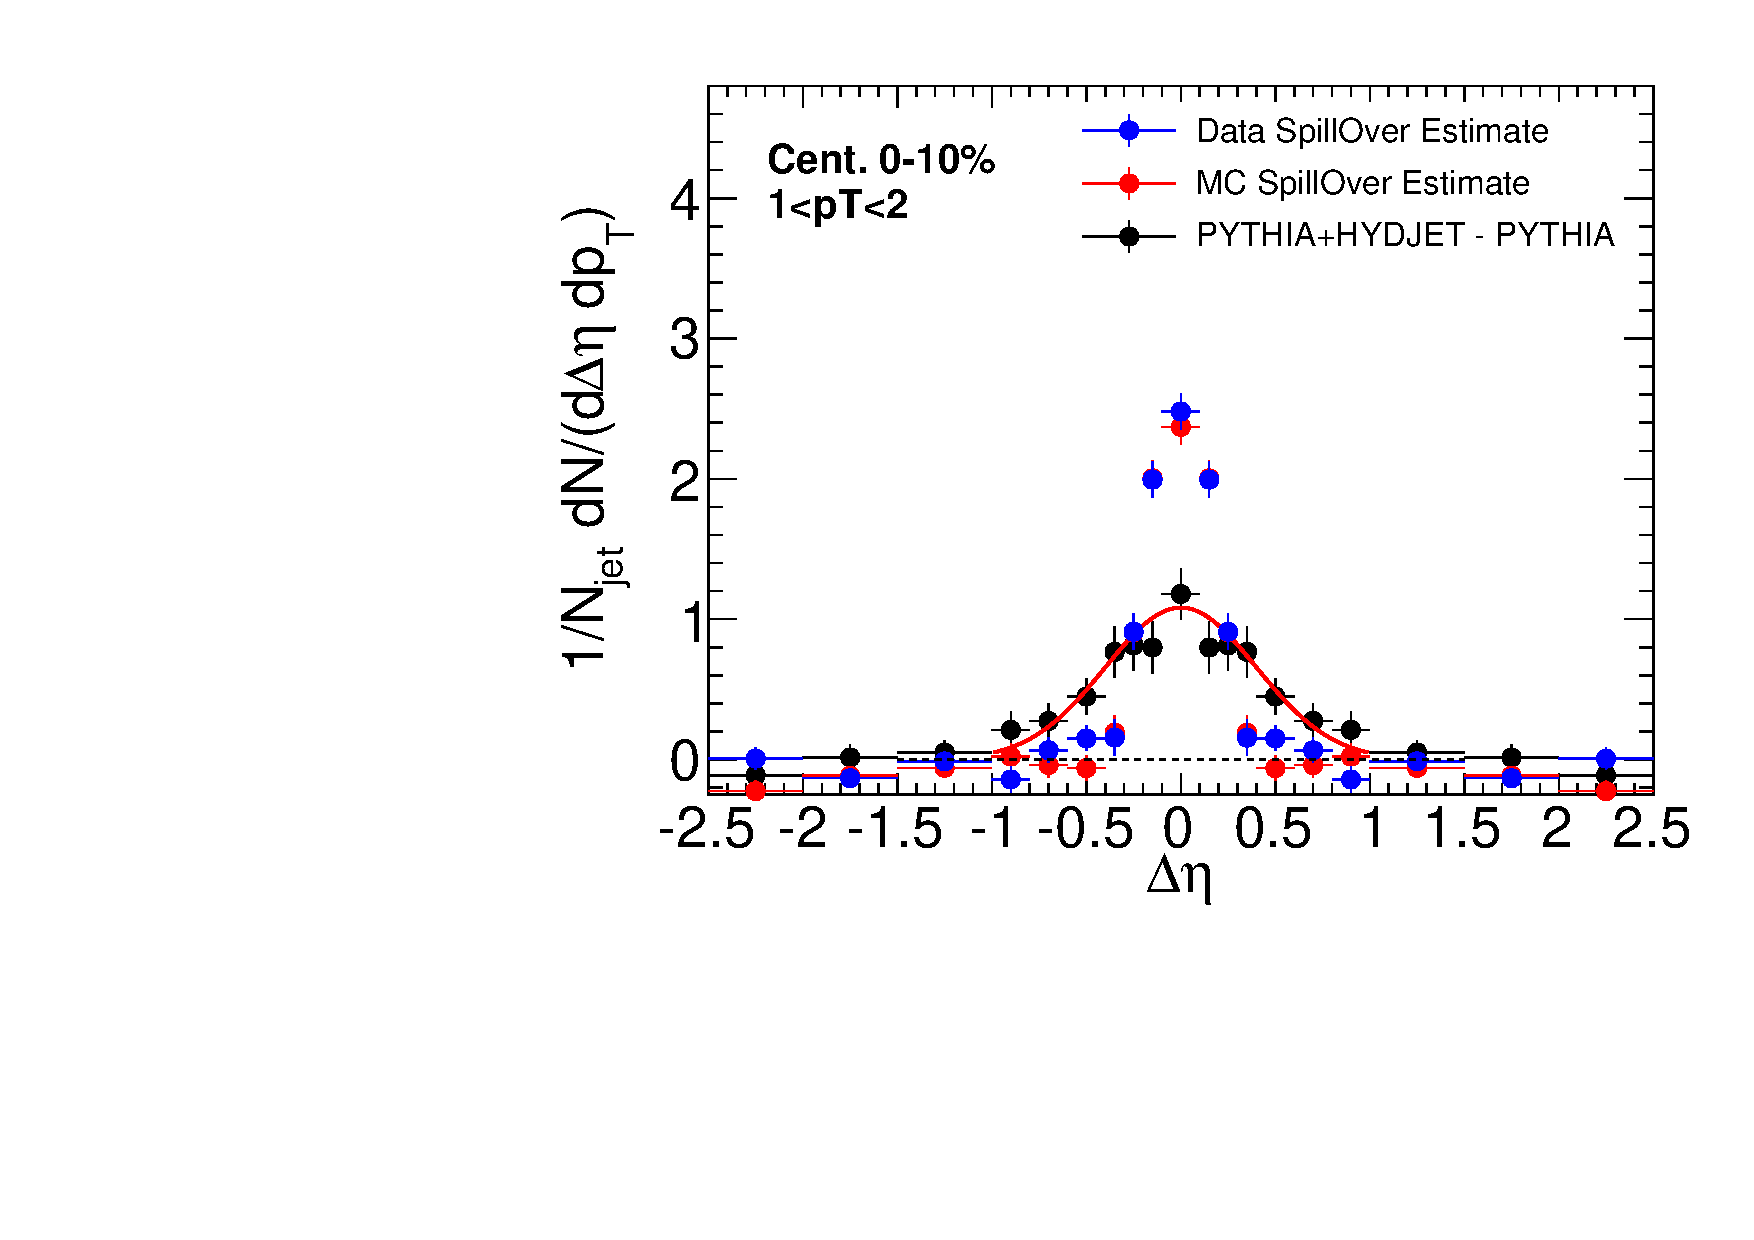
\includegraphics[width=0.49\textwidth]{figures/JFF_SpillOver/Data_Closures_TrkPt1_TrkPt2.pdf}
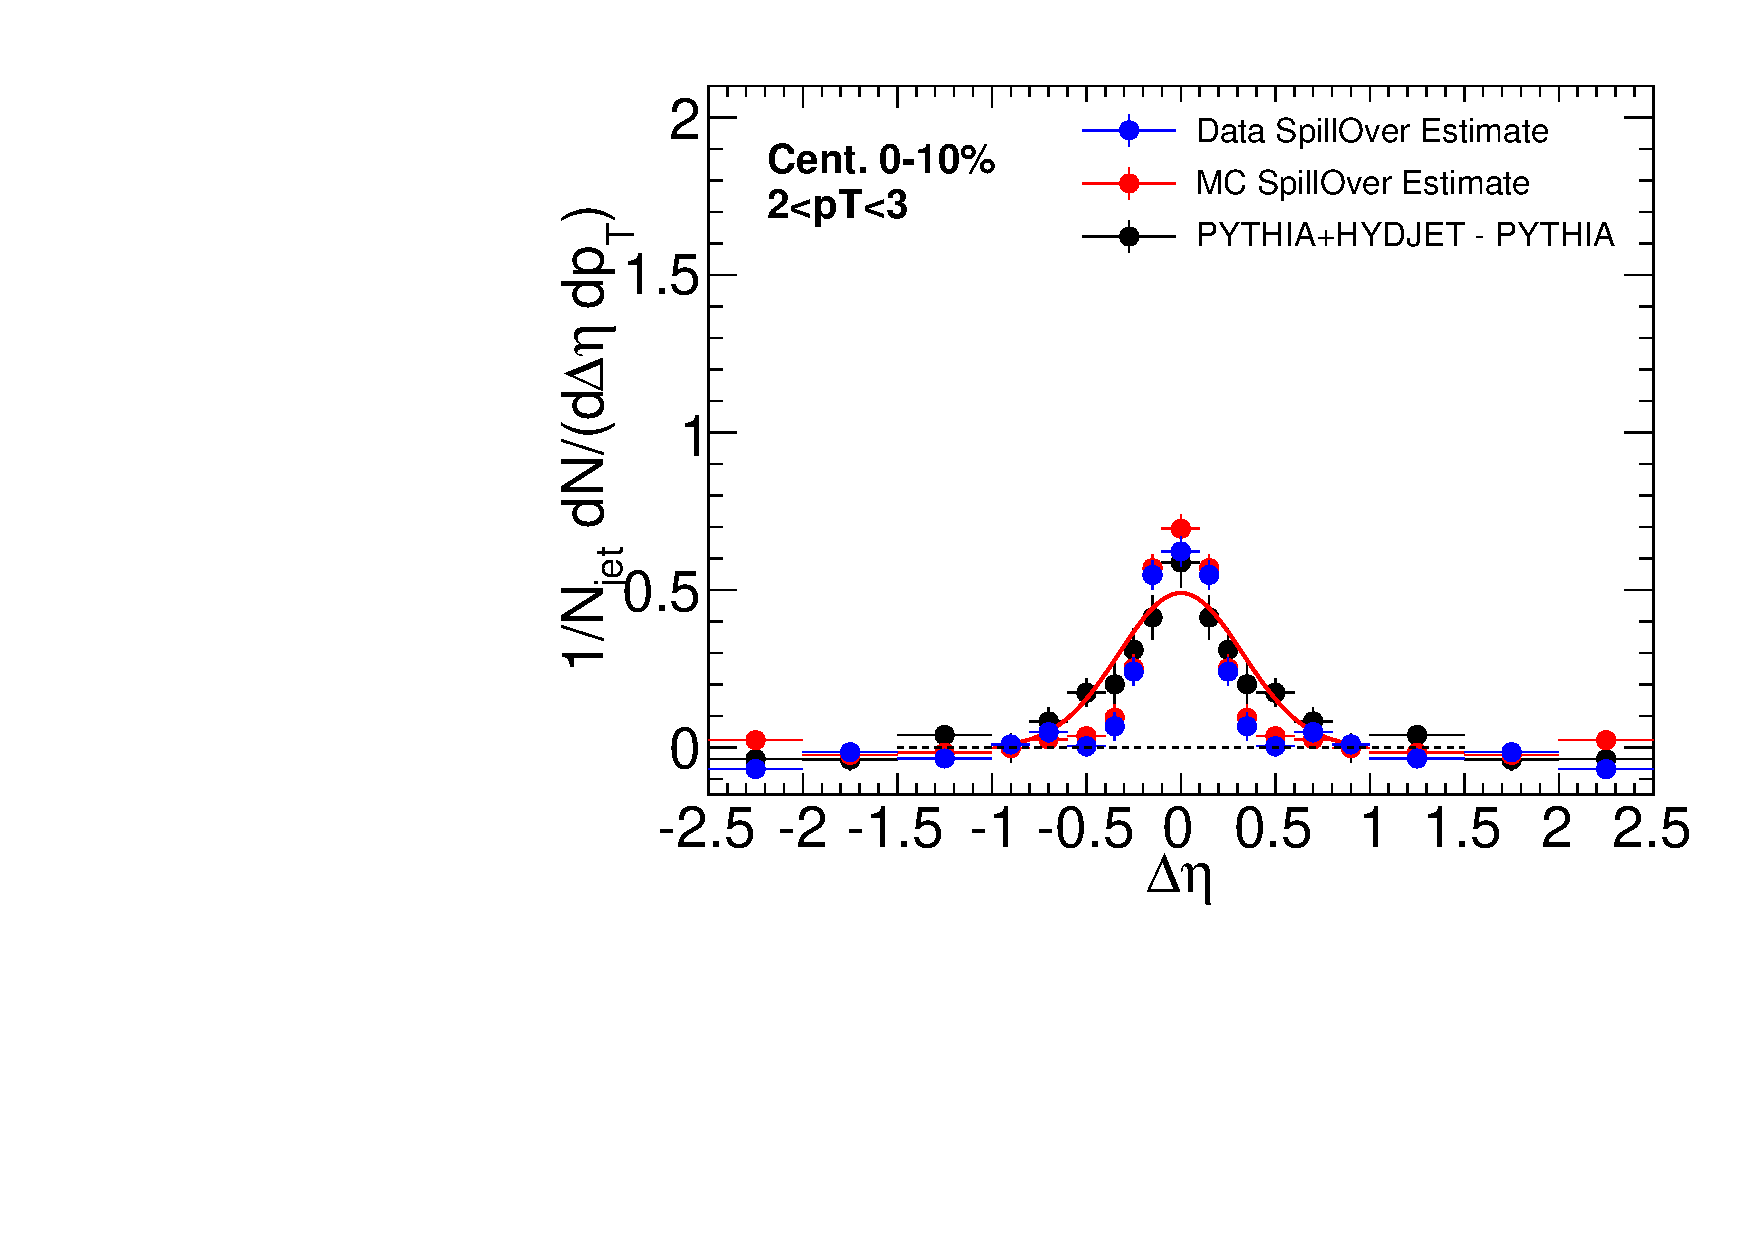
\includegraphics[width=0.49\textwidth]{figures/JFF_SpillOver/Data_Closures_TrkPt2_TrkPt3.pdf}
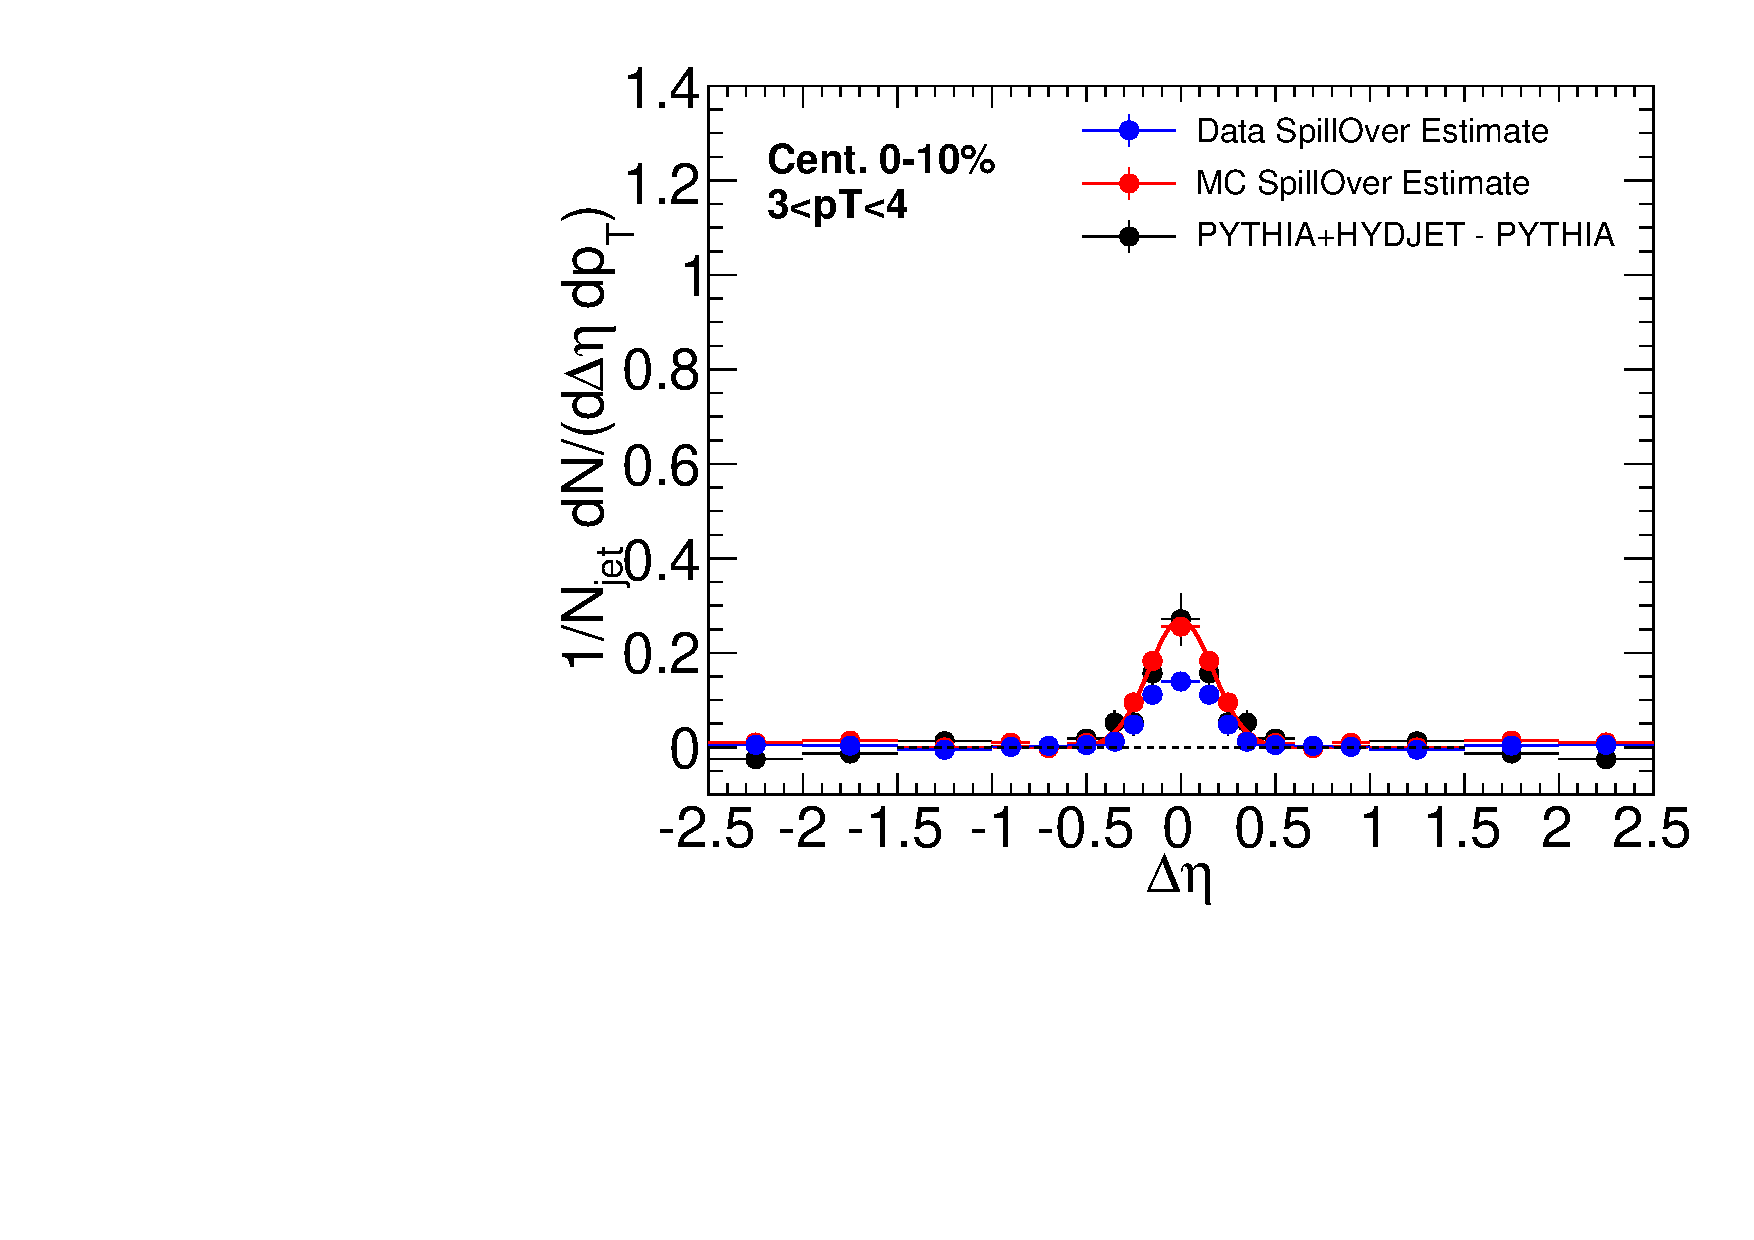
\includegraphics[width=0.49\textwidth]{figures/JFF_SpillOver/Data_Closures_TrkPt3_TrkPt4.pdf}
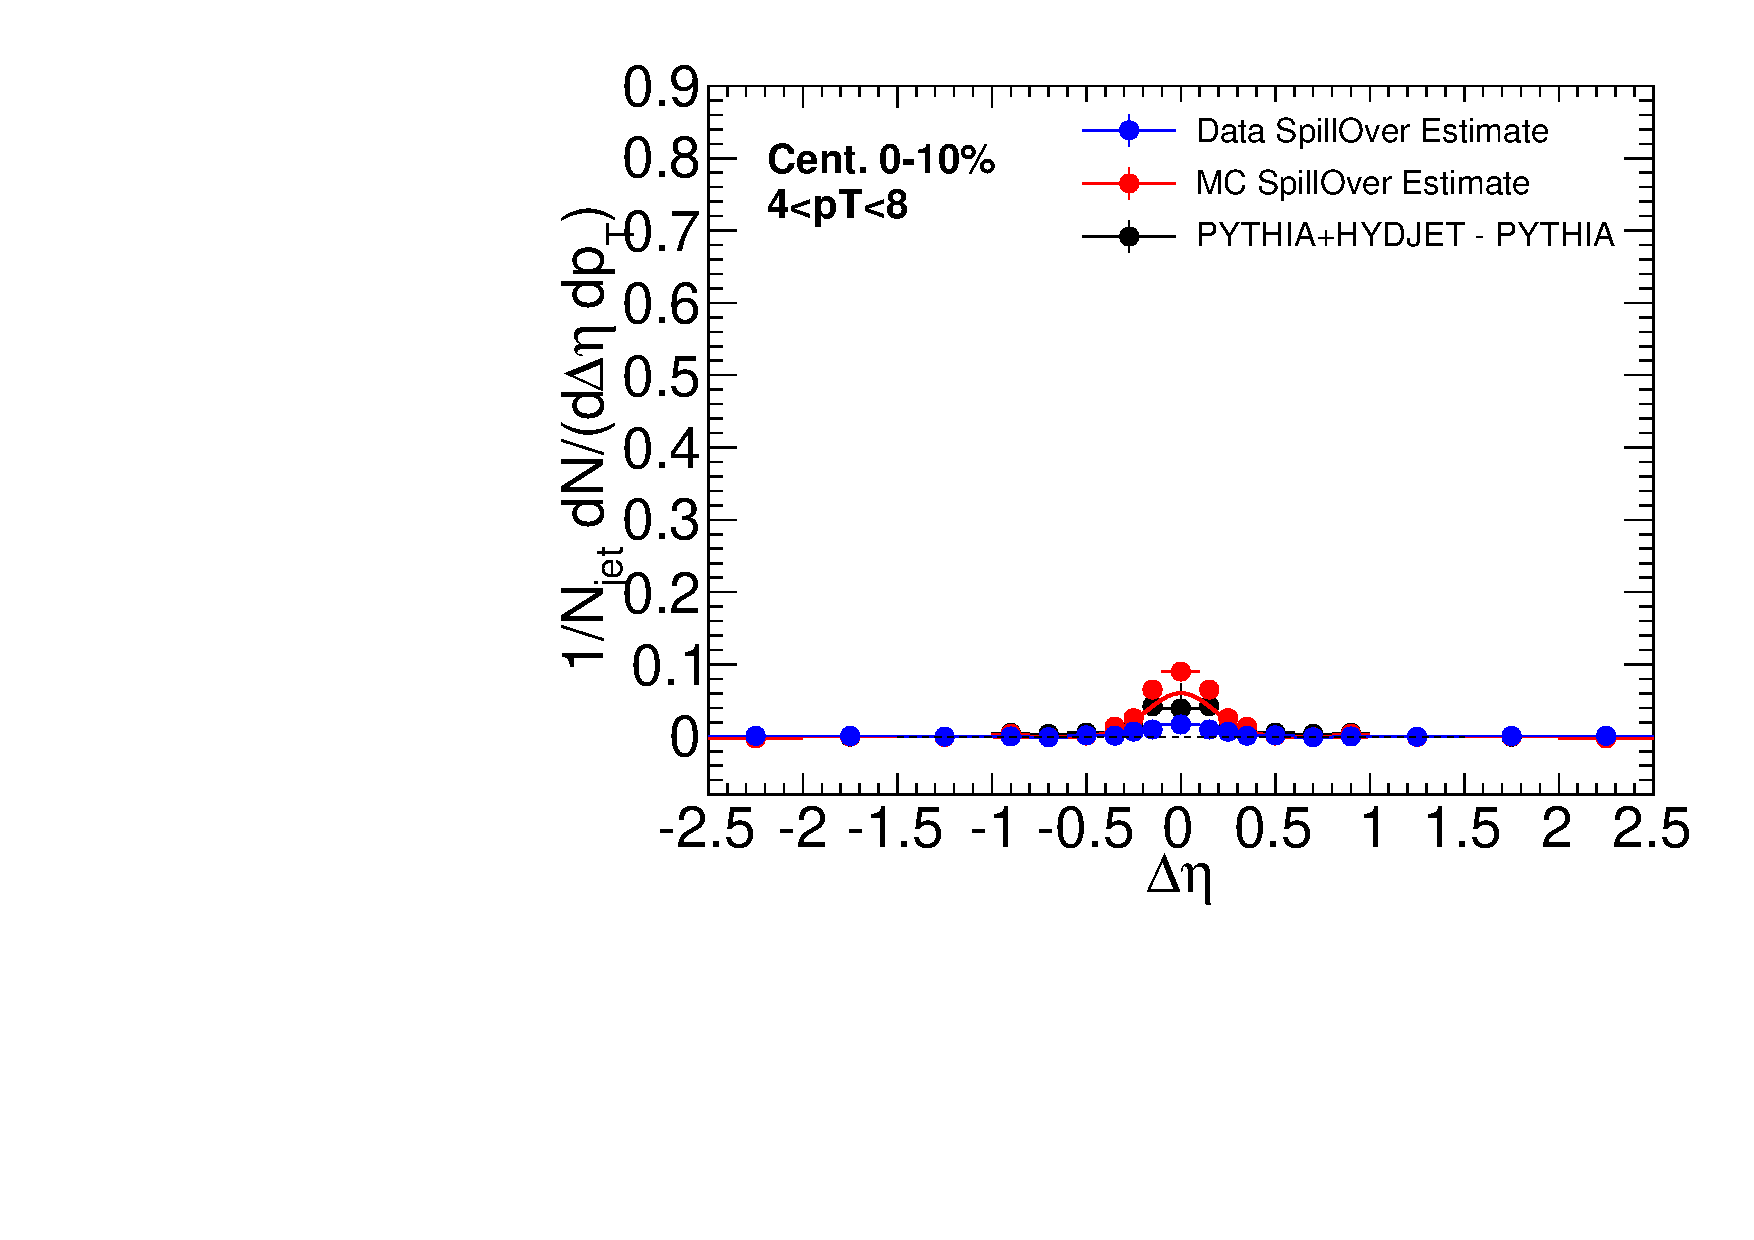
\includegraphics[width=0.49\textwidth]{figures/JFF_SpillOver/Data_Closures_TrkPt4_TrkPt8.pdf}
\caption[Data-driven check of correlated $\Delta\eta$ yields attributed to background fluctuation bias]{Correlated yield $\Delta\eta$ due to background fluctuation bias as simulated with pp jets embedded in Minimum Bias events (blue points) compared to the effect applying the same technique with {\sc pythia}  jets in {\sc hydjet}  minimum bias events, as well as in full {\sc pythia+hydjet} simulation (black points with red fit line).}
\label{fig:data_spill_bins}
\end{center}
\end{figure}
 
The background fluctuation bias could also be sensitive to the same calorimeter nonlinearity bias that necessitates fragmentation-jet energy corrections.  To study this question and validate the uncertainty associated with this correction, we separately study the effect for quark jets and gluon jets, as shown in Figure~\ref{fig:quark_gluon_closure}.  This study is limited by statistics, but deviations (or fluctuations) in the bias for quark versus gluon jets are are within the 50\% systematic uncertainty assigned.  


                  \begin{figure}[hbtp]
                  \begin{center}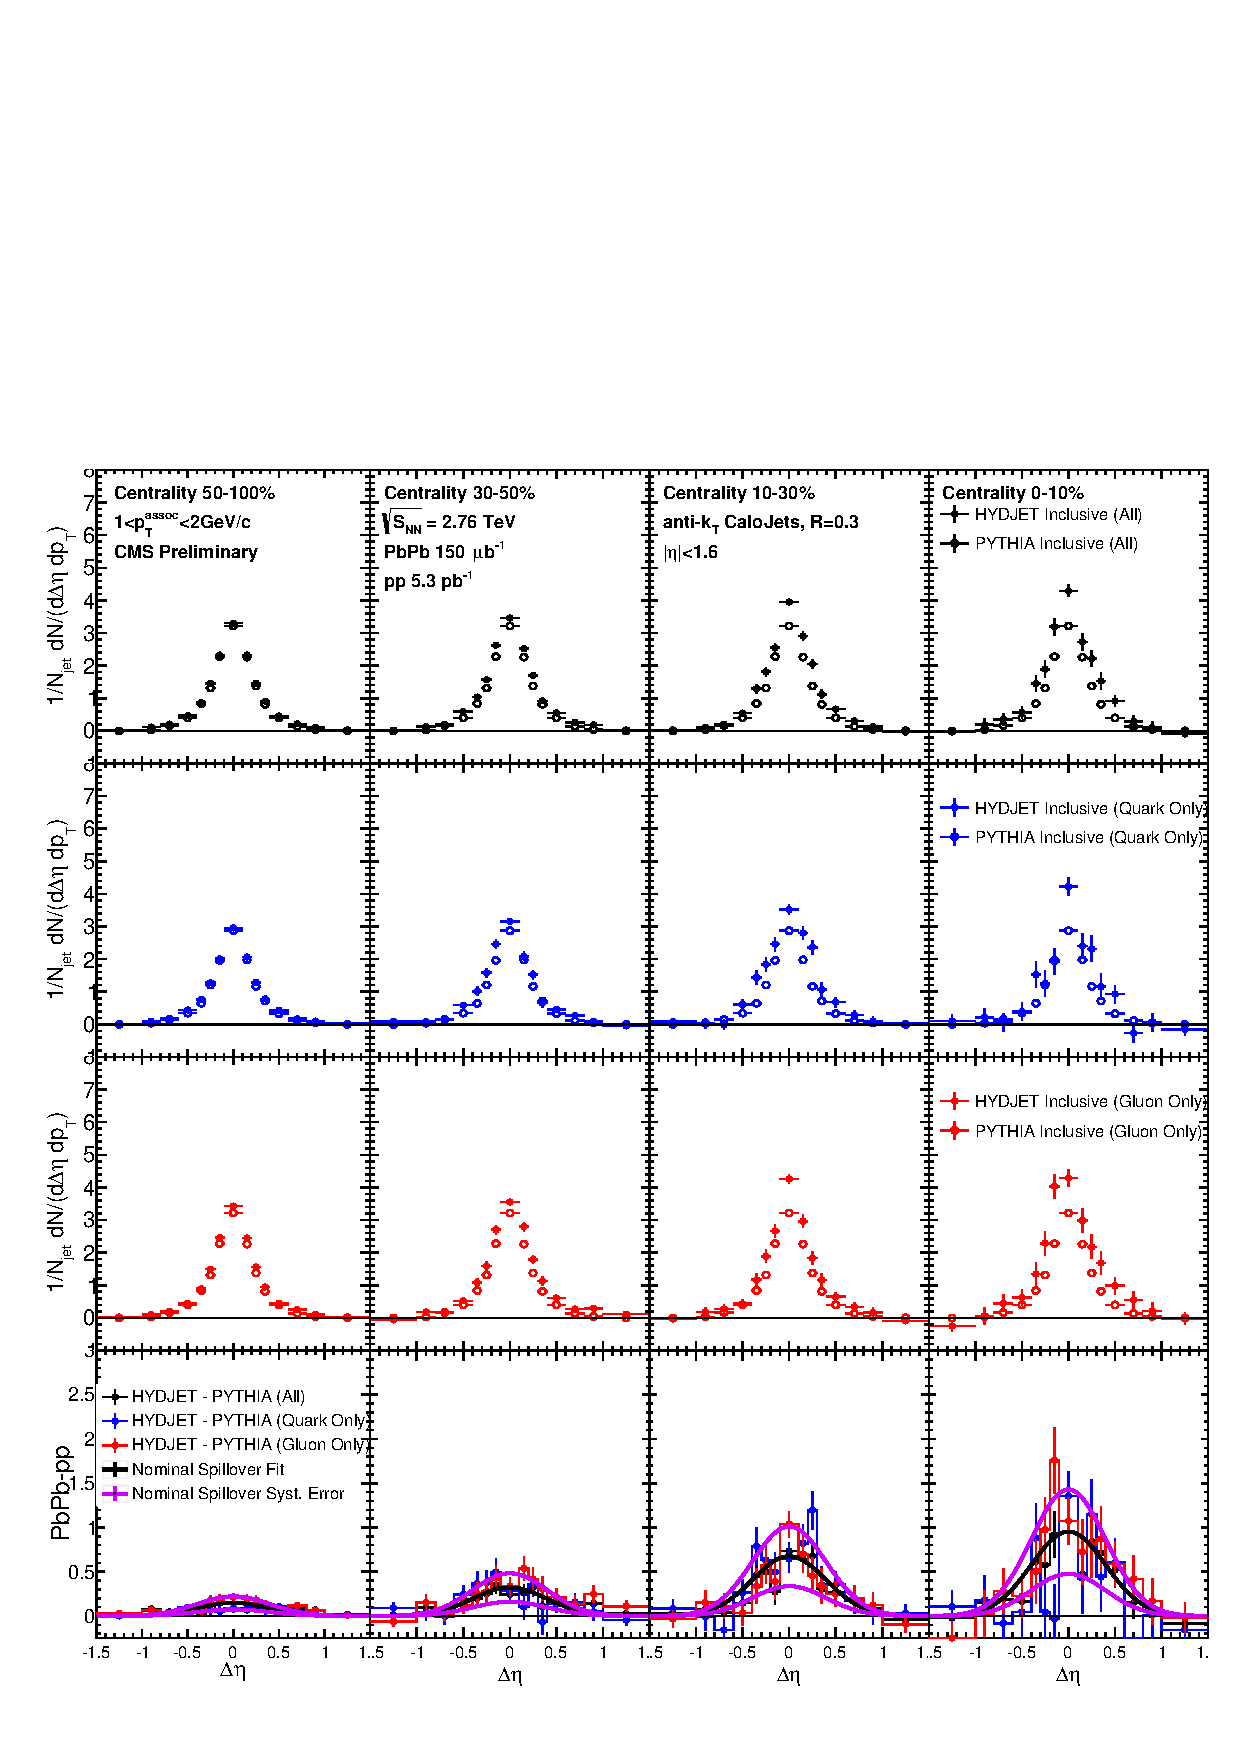
\includegraphics[width=0.99\textwidth]{figures/JFF_SpillOver/QuarkGluonComparison.pdf}
                  \caption[Comparison of background selection bias effect for quark verus gluon jets]{Comparison of magnitude of background selection bias effect for quark and gluon jets versus our nominal sample.  Jet selection is inclusive in all cases.}
                    \label{fig:quark_gluon_closure}
                    \end{center}
                    \end{figure}


                 

\clearpage

	
\subsection{Evaluation of systematic uncertainties}

A number of sources of systematic uncertainty have been discussed in presenting jet and track reconstruction and the jet-track correlation analysis procedure.  To estimate the total systematic uncertainty in these measurements, these contributions are added in quadrature.  A brief summary of all systematic uncertainty contributions, together with the procedure used to estimate their magnitude follows.  The contributions from each source (relative to jet peak signal) are summarized in Tables~\ref{tab:sys1}--\ref{tab:sys3}.

\subsubsection{Systematic uncertainties related to jet reconstruction}

Jet reconstruction-related sources of systematic uncertainty in this analysis include the two reconstruction biases as discussed above, as well uncertainty associated with the jet energy scale (JES) evaluation.  We consider three sources of uncertainty on the JES:  (1) differences in calorimeter response for quark versus gluon jets, meaning that medium-induced changes in jet flavor could result in either over-correction or under-correction of jet energy and a resulting bias in jet selection (evaluated via Monte Carlo non-closure for quark and gluon jets); (2) possible differences between data and simulation; (3) uncertainty due to quenching effects not included in our {\sc hydjet} simulation.  To evaluate how each of these sources of JES uncertainty affects final correlations, we vary jet selection threshold by the combined uncertainty, and then quantify the resulting differences in the final correlations as a measure of the combined residual JES uncertainty. Since all the measured correlations are studied per-reconstructed jets, the jet reconstruction efficiency does not contribute to the systematic uncertainty of this measurement.

\subsubsection{Systematic uncertainties related to tracking and tracking efficiency corrections}

The tracking efficiency correction uncertainty is estimated from the ratio of corrected reconstructed yields and generated yields by using generator level charged particles as a ``truth'' reference.  To account for the possible track reconstruction differences in data and simulation, a residual uncertainty in track reconstruction efficiency and fake rate corrections is also estimated.   

\subsubsection{Systematic uncertainty associated with pair acceptance correction and event decomposition}

Uncertainty arising from pair-acceptance effects is estimated by considering the sideband asymmetry after dividing by the mixed-event background.  Each sideband region of the final $\Delta\eta$ distribution ($-2.5<\Delta\eta<-1.5$ and $1.5<\Delta\eta<2.5$) is separately fit with a horizontal line after background subtraction.  The greater of these two deviations from zero is assigned as systematic error.  Uncertainties resulting from the background subtraction are determined by considering the average point-to-point deviation in two parts of the sideband region ($1.5<|\Delta\eta|<2.0$ and $2.0<|\Delta\eta|<2.5$) after background subtraction.  The derivations of both of these sources of uncertainty are illustrated in Appendix~\ref{app:err_me_bkg}.  In PbPb data this background subtraction uncertainty is greatest for the most central events (0--10\%) and the lowest track $p_{\rm T}$ bin where the background is most significant compared to the signal level, and decreases for less central collisions and for higher $p_{\rm T}$ tracks ($p_{\rm T}^{\rm trk} > 2$ GeV).  

\subsubsection{Summary of systematic uncertainties}

The contributions to total systematic uncertainty from each of the sources described above are given in Tables~\ref{tab:sys1}--\ref{tab:sys3}. Table~\ref{tab:sys1} gives uncertainty evaluations for correlation studies at 2.76 TeV, while Table~\ref{tab:sys2} gives the same for studies at 5.02 TeV.  Finally, Table~\ref{tab:sys3} gives uncertainty evaluations for balanced ($A_{\rm J} < 0.22$) and unbalanced ($A_{\rm J} > 0.22$) dijet events in momentum balance studies at 2.76 TeV.  

\begin{table}[htbp]
\begin{center}

\caption[Systematic uncertainties for particle density correlation studies at 2.76 TeV]{Systematic uncertainties in the measurement of the jet-track correlations in PbPb and pp collisions at 2.76 TeV, as percentage of the total measured correlated yield. The numbers presented in this table summarize the range of values of systematic uncertainty (as a function of $p_{\rm T}^{\rm trk}$) for different centrality bins.}
\label{tab:sys1}
\begin{tabular}{c|cccc|c}
\hline
\hline
Source & 0--10\% &  10--30\% & 30--50\% & 50--100\% &  pp \\ \hline
\hline

Background fluctuation bias             & 3--12\% & 2--7\% & 1--5\% & 0--1\% &  -- \\
Jet fragmentation function bias       & 0--2\% &    0--2\% &   0--2\% & 0--2\% &  0--2\% \\
Residual jet energy scale                                   & 3\% &    3\% &   3\% &    3\% &   3\% \\
Tracking efficiency uncertainty          & 4\% & 4\% & 4\% & 4\% &   3 \%  \\
Residual track efficiency corr.              &    5\% &    5\% &    5\% &    5\% &    5\% \\
Pair acceptance corrections                  & 5--9\% & 5--9\% & 4--8\% & 2--6\% &  2--3\% \\
Background subtraction                       & 2--5\% & 2--5\% & 2--5\% & 2--5\% &  1--2\% \\


\hline
Total                                        & 9--17\% & 9--14\% & 8--13\% & 8--10\% & 7--8\% \\

\hline


\end{tabular}
\end{center}
\end{table}


\begin{table}[htbp]
\begin{center}
	
\caption[Systematic uncertainties for particle density correlation studies at 5.02 TeV]{Systematic uncertainties in the measurement of the jet track correlations in PbPb and pp collisions at 5.02 TeV. The numbers presented in this table summarize typical range of systematic uncertainty as a function of collision centrality.  The upper limits of the cited values correspond to uncertainties at lowest $p_{\rm T}^{\rm trk}$, and uncertainties decrease with rising $p_{\rm T}^{\rm trk}$.}

\begin{tabular}{c|ccccc}
\hline
\hline
Source & 0--10\% &  10--30\% & 30--50\%& 50--100\% & ppRef \\ 
\hline
Background fluctuation bias              & 0--10\%    & 0--5\%  &        0--2\%  &       0--1\% & -- \\
Background fluctuation bias residual      & 0--2\% &       0--3\% &     0--1\% &     0--1\%&       --\\
JFF bias                                         & 3--5\%      & 3--4\% &        3--4\%&       3--4\%    &    3\% \\
Residual JES                                   & 4\% &       4\% &               4\% &            4\% &          4\% \\  
Tracking efficiency uncertainty          & 1\% &             1\%&         1\%&           1\% &        1\%  \\
Residual tracking efficiency              &    5\% &                5\%&      5\%&            5\% &         5\% \\
Pair-acceptance corrections              & 1--5\% &      1--4\% &     1--4\% &       1--4\% &       1--2\% \\
Event decomposition                     & 1--9\% &       0--4\% &     0--4\% &     0--3\%&       0--3\% \\
\hline
Total                                        & 7--16\%     & 7--11\%     & 7--9\%  & 7--9\% &        7--8\% \\
\hline
\hline
\end{tabular}
\label{tab:sys2}
\end{center}
\end{table}





\begin{table}[htbp]

\begin{center}
\caption[Systematic uncertainties for balanced and unbalanced dijets in transverse momentum distribution studies at 2.76 TeV]{This table summarizes the systematic uncertainties in the measurement of the $p_{\rm T}^{\rm trk}$ correlations in PbPb and pp collisions at 2.76 TeV. Upper and lower limits are shown as a function of collision centrality.  Upper values correspond to the uncertainties at lowest $p_{\rm T}^{\rm trk}$.}
\label{tab:sys3}
\begin{tabular}{c|ccccc}
\hline
\hline

Source & 0--30\% &   30--50\% & 50--100\% & pp \\ \hline
\hline
Balanced jet selection ($A_{\rm J} < 0.22$):\\
\hline
Background fluctuations                       & 1--8\%  & 1--3\% & 0--1\% & -- \\
JFF bias and jet swapping               & 0--2\%  &   0--2\% & 0--2\% &    0--2\% \\
Residual JES                                   & 3\% &      3\% &    3\% &    3\% \\
Tracking efficiency         & 4\%  & 4\% & 4\% & 3 \%  \\
Residual track efficiency corr.              &    5\%  &    5\% &    5\% &    5\% \\
Pair acceptance corrections                  & 5--9\%  & 4--8\% & 2--6\% & 2--3\% \\
Event decomposition                      & 2--5\% & 2--5\% & 2--5\% & 1--2\% \\
\hline
Total                                        & 9--15\%  & 8--13\% & 8--10\% & 7--8\% \\
\hline
\hline
Unbalanced jet selection ($A_{\rm J} > 0.22$):\\
\hline
Background fluctuations                       & 1--10\% &  1--5\% & 0--2\% & -- \\
JFF bias and jet swapping               & 0--2\% &      0--2\% & 0--2\% &    0--2\% \\
Residual JES                                   & 3\% &     3\% &    3\% &    3\% \\
Tracking efficiency           & 4\% & 4\% & 4\% & 3 \%  \\
Residual track efficiency corr.              &    5\% &    5\% &    5\% &    5\% \\
Pair acceptance corrections                  & 5--9\%  & 4--8\% & 2--6\% & 2--3\% \\
Event decomposition                    & 2--5\% &  2--5\% & 2--5\% & 1--2\% \\
\hline
Total                                        & 9--16\%  & 8--13\% & 8--10\% & 7--8\% \\

\hline
\hline

\end{tabular}
\end{center}
\end{table}



\clearpage

\section{Discussion of results}
\label{sec:Results}


Jet-track correlation studies can produce measurements of the density of particles (in each $p_{\rm T}^{\rm trk}$ class) with respect to the jet axis and can also, by creating correlations weighted per-track by its $p_{\rm T}^{\rm trk}$, produce measurements of the distribution of $p_{\rm T}^{\rm trk}$ in the event as a whole.  Both types of measurements are presented here, for inclusive selections of jets with $p_{\rm T} > 120$ GeV at 2.76 TeV and 5.02 TeV, and for high-$p_{\rm T}$ dijet events at 2.76 TeV.  First, particle density correlation results are presented in Secs.~\ref{sec:inc_corr}-~\ref{sec:dijet_corr}.  Next, $p_{\rm T}^{\rm trk}$ distributions are used to extract measurements of jet shapes (the transverse momentum profiles of jets) in Sec.~\ref{sec:jet_shapes}.  Finally, in Sec.~\ref{sec:dijet_mpt}, $p_{\rm T}^{\rm trk}$ distributions are used to decompose and analyze the hemisphere momentum balance in dijet events.

\subsection{Inclusive jet particle density correlation results}
\label{sec:inc_corr}


Particle density correlation studies allow for the detailed characterization of jet fragmentation, and of medium-induced modifications to jet fragmentation in PbPb data (as a function of collision centrality) compared to pp data.  The analysis procedure described in Sec.~\ref{sec:JetTrack} results in fully-corrected 2D jet peaks in $\Delta\eta-\Delta\phi$, which may then be projected to obtain the distribution of particles in each $p_{\rm T}^{\rm trk}$ class as a function of $\Delta\eta$ or $\Delta\phi$.  The top panels of Figs.~\ref{fig:Inclusive_dEta1}-\ref{fig:Inclusive_dPhi4} show these $\Delta\eta$ and $\Delta\phi$ distributions (projected over $|\Delta\phi| < 1$ and $|\Delta\eta| < 1$, respectively) for 2.76 TeV pp data and PbPb data in each $p_{\rm T}^{\rm trk}$ range from 1--2 GeV (Fig.~\ref{fig:Inclusive_dEta1}-\ref{fig:Inclusive_dPhi1}) up to 4--8 GeV (Fig.~\ref{fig:Inclusive_dEta4}-\ref{fig:Inclusive_dPhi4}).  The bottom panels of these figures show the differences PbPb--pp for illustration of medium modifications to jet fragmentation patterns.  In both the $\Delta\eta$ and $\Delta\phi$ dimensions, centrality-dependent excesses of soft (low-$p_{\rm T}^{\rm trk}$) particles are evident.  These exhibit the greatest modifications in the most central PbPb collisions, decreasing with centrality until the most peripheral collisions show little modification when compared to pp data.  These excesses decrease with increasing $p_{\rm T}^{\rm trk}$, until in the 4-8 GeV range the enhancements evident at lowest-$p_{\rm T}^{\rm trk}$ reverse to possible slight depletion.  In both $\Delta\eta$ and $\Delta\phi$ dimensions, the soft excesses exhibit a gaussian-like distribution around the jet axis, while also extending to large angles $\Delta\eta = 1$ and $\Delta\phi = 1$ at lowest $p_{\rm T}^{\rm trk}$.  

Figures~\ref{fig:yield_deta_stacked} and~\ref{fig:yield_dphi_stacked} show the corresponding $\Delta\eta$ and $\Delta\phi$ distributions at 5.02 TeV.  Here, the distribution of particles in each $p_{\rm T}^{\rm trk}$ class are stacked (with lowest-$p_{\rm T}^{\rm trk}$ particles on top), and pp data shown separately at left.  Again the differences PbPb--pp are shown in bottom panels to illustrate the medium modifications, and exhibit similar qualitative trends to those described above for 2.76 TeV results.  Results may also be presented as a function of radial distance from the jet axis $\protect\Delta r = \sqrt{\Delta\eta^{2}+\Delta\phi^{2}}$.  Figure~\ref{fig:yield_dr_stacked} presents charged particle yields, differentially in $p_{\rm T}^{\rm trk}$, as a function of $\protect\Delta r$.  For comparison, the bottom row of each plot shows the difference, PbPb minus pp.  This shows the particles contributing to a jet fragmentation function measurement within a given radius from a jet, and illustrates the radial dependence of modifications extending to at least $\protect\Delta r = 1$.  


\begin{figure}[hbt] 
\begin{center} 
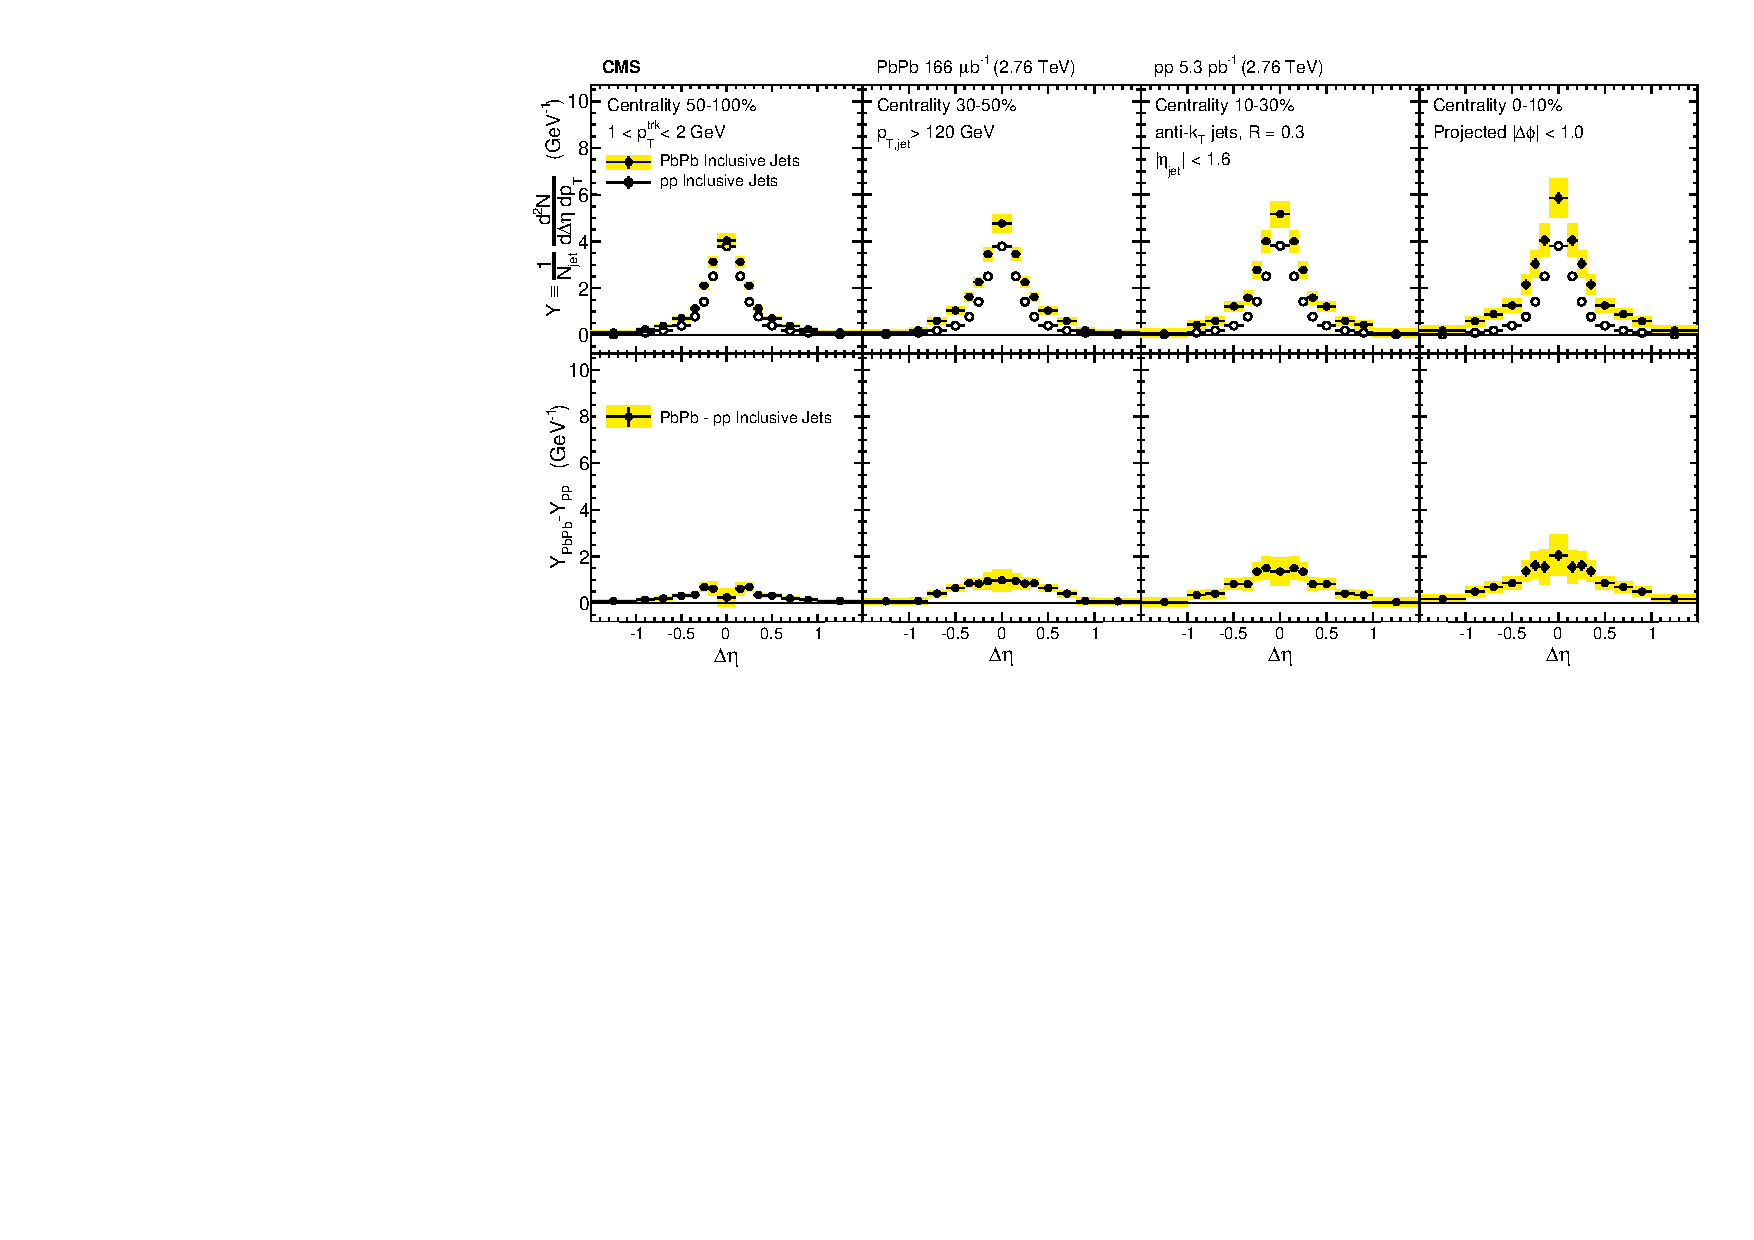
\includegraphics[width=0.99\textwidth]{figures/Results/PAS_Figure_3_TrkPt1_TrkPt2.pdf}
\caption[Inclusive jet $\Delta\eta$ correlations for tracks with $1 < p_{\rm T}^{\rm trk} < 2$ GeV at 2.76 TeV]{Symmetrized $\protect\Delta\eta$ distributions (projected over $|\Delta\phi| < 1$) of background-subtracted particle yields correlated to PbPb and pp inclusive jets with $p_{\rm T}>$ 120 GeV are shown in the top panels for tracks with 1 $ < p_{\rm T}^{\rm trk} < $ 2 GeV.  The difference in PbPb and pp per-jet yields is shown in the bottom panels. The total systematic uncertainties are shown as shaded boxes, and statistical uncertainties are shown as vertical bars (often smaller than the symbol size).}
\label{fig:Inclusive_dEta1}
\end{center} 
\end{figure} 

\begin{figure}[hbt] 
\begin{center} 
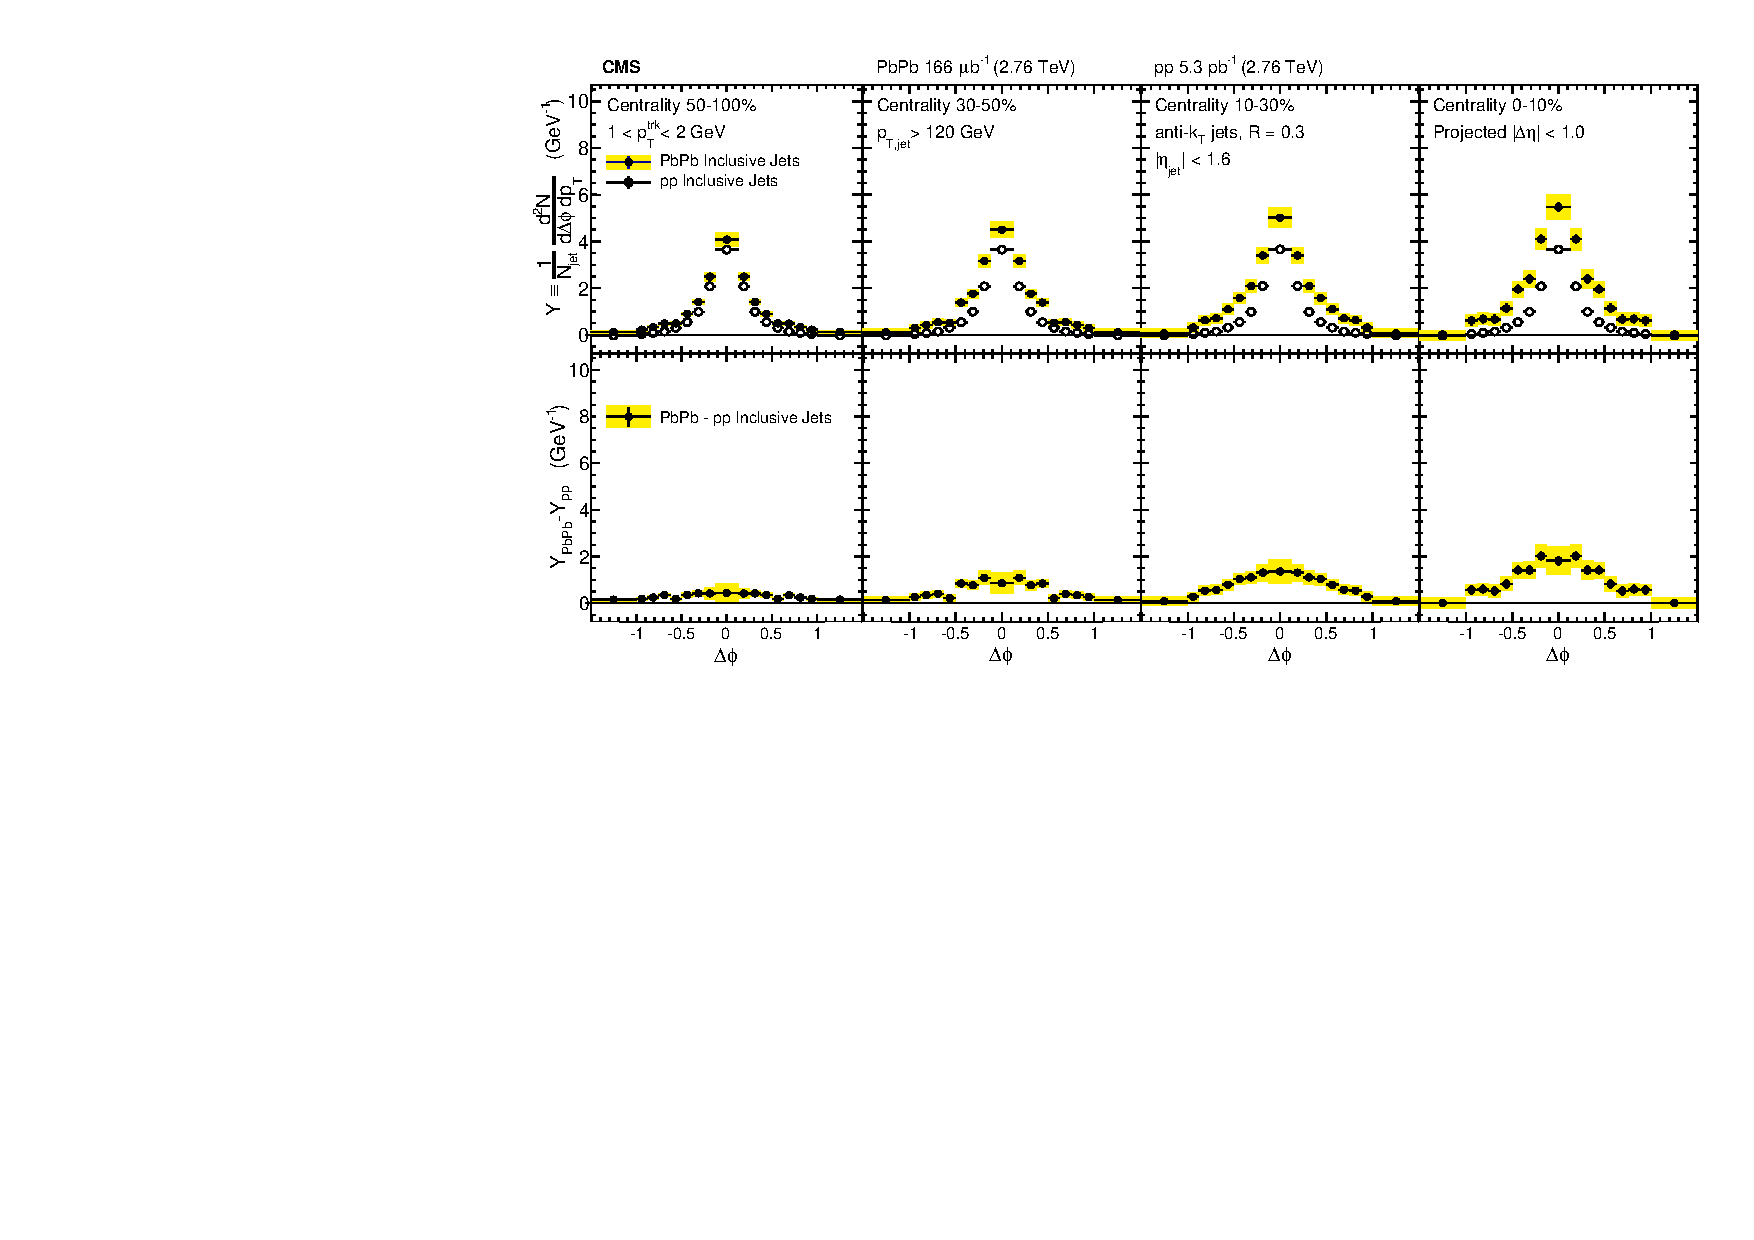
\includegraphics[width=0.99\textwidth]{figures/Results/PAS_Figure_4_TrkPt1_TrkPt2.pdf}
\caption[Inclusive jet $\Delta\phi$ correlations for tracks with $1 < p_{\rm T}^{\rm trk} < 2$ GeV at 2.76 TeV]{Symmetrized $\protect\Delta\phi$ distributions  (projected over $|\Delta\eta| < 1$) of background-subtracted particle yields correlated to PbPb and pp inclusive jets with $p_{\rm T} >$ 120 GeV are shown in the top panels for tracks with 1 $ < p_{\rm T}^{\rm trk} < $ 2 GeV.  The difference in PbPb and pp per-jet yields is shown in the bottom panels. The total systematic uncertainties are shown as shaded boxes, and statistical uncertainties are shown as vertical bars (often smaller than the symbol size).}
\label{fig:Inclusive_dPhi1} 
\end{center} 
\end{figure} 



\begin{figure}[hbt] 
\begin{center} 
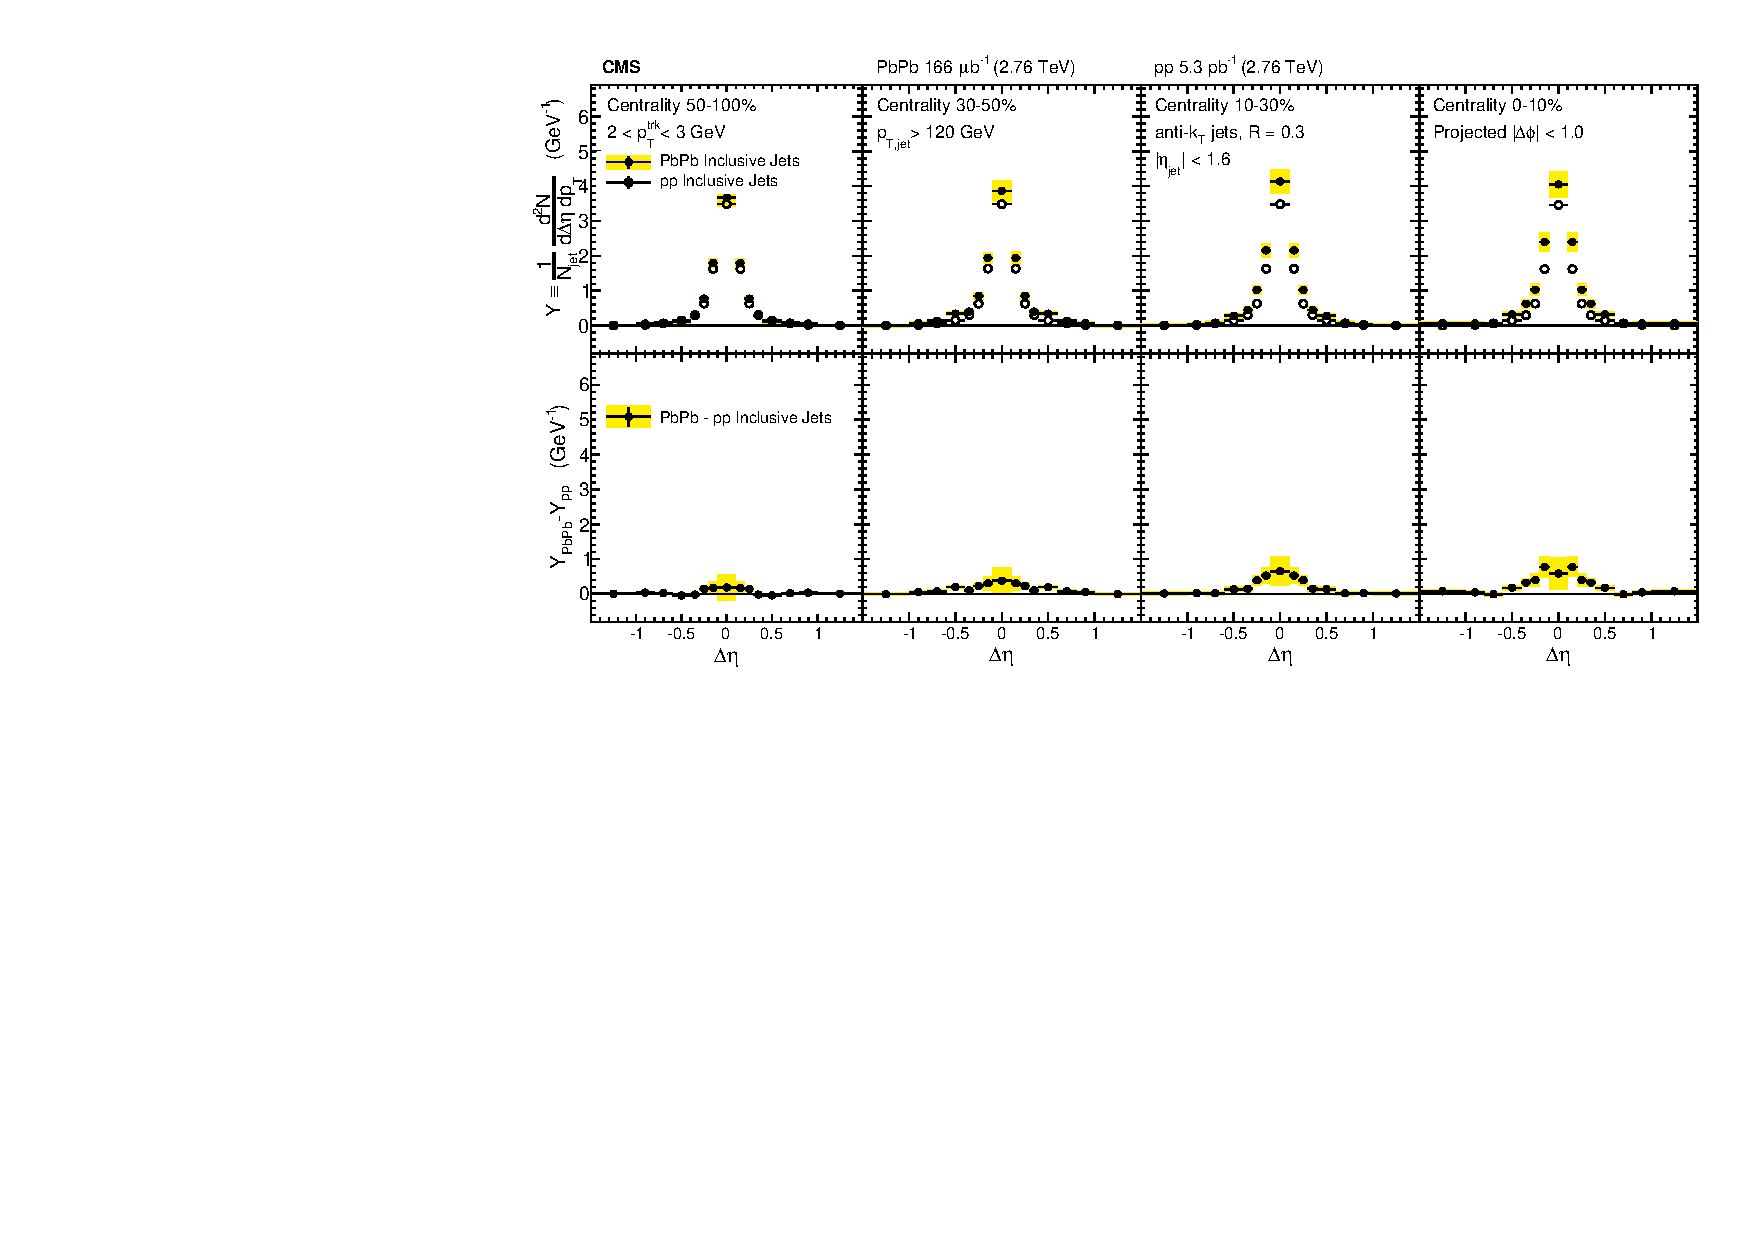
\includegraphics[width=0.99\textwidth]{figures/Results/PAS_Figure_3_TrkPt2_TrkPt3.pdf}
\caption[Inclusive jet $\Delta\eta$ correlations for tracks with $2 < p_{\rm T}^{\rm trk} < 3$ GeV at 2.76 TeV]{Symmetrized $\protect\Delta\eta$ distributions (projected over $|\Delta\phi| < 1$) of background-subtracted particle yields correlated to PbPb and pp inclusive jets with $p_{\rm T}>$ 120 GeV are shown in the top panels for tracks with 2 $ < p_{\rm T}^{\rm trk} < $ 3 GeV.  The difference in PbPb and pp per-jet yields is shown in the bottom panels. The total systematic uncertainties are shown as shaded boxes, and statistical uncertainties are shown as vertical bars (often smaller than the symbol size).}
\label{fig:Inclusive_dEta2}
\end{center} 
\end{figure} 

\begin{figure}[hbt] 
\begin{center} 
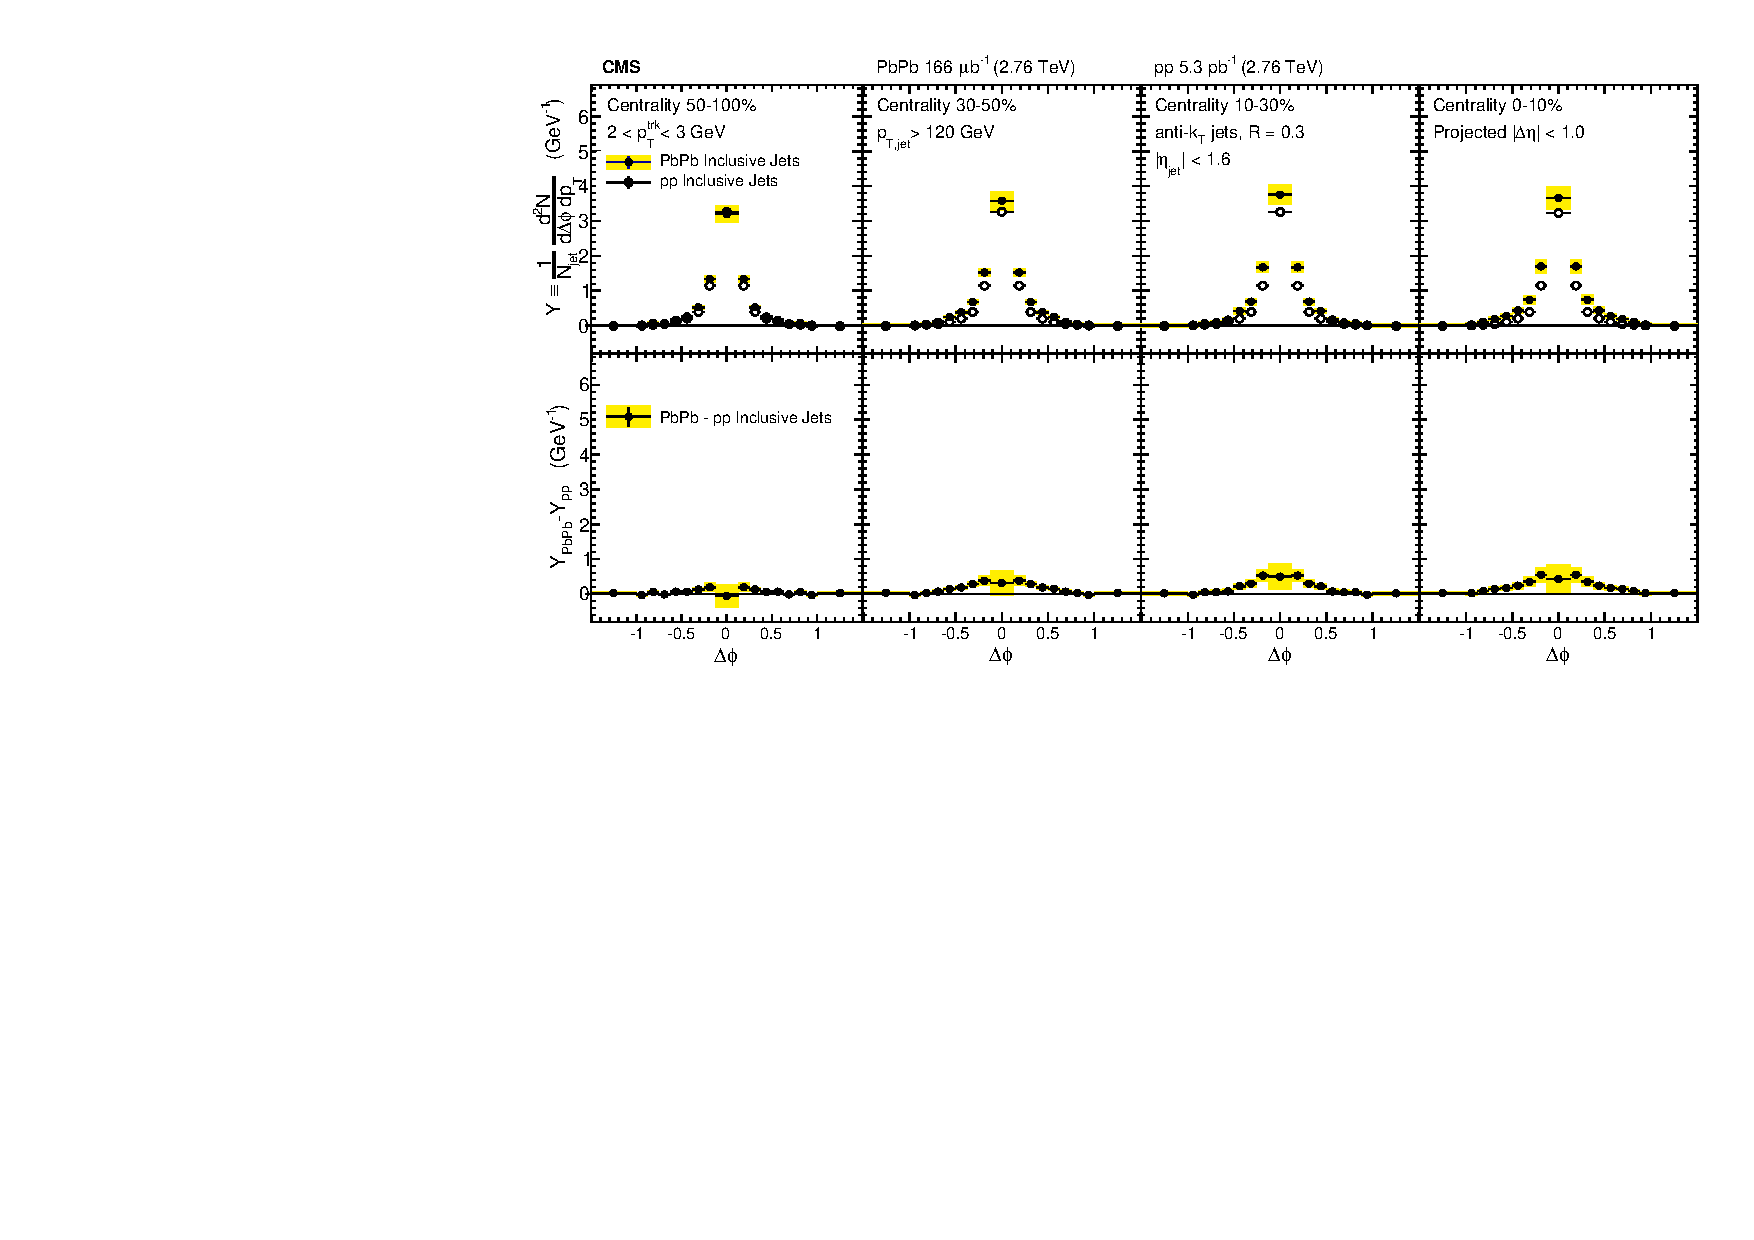
\includegraphics[width=0.99\textwidth]{figures/Results/PAS_Figure_4_TrkPt2_TrkPt3.pdf}
\caption[Inclusive jet $\Delta\phi$ correlations for tracks with $2 < p_{\rm T}^{\rm trk} < 3$ GeV at 2.76 TeV]{Symmetrized $\protect\Delta\phi$ distributions  (projected over $|\Delta\eta| < 1$) of background-subtracted particle yields correlated to PbPb and pp inclusive jets with $p_{\rm T} >$ 120 GeV are shown in the top panels for tracks with 2 $ < p_{\rm T}^{\rm trk} < $ 3 GeV.  The difference in PbPb and pp per-jet yields is shown in the bottom panels. The total systematic uncertainties are shown as shaded boxes, and statistical uncertainties are shown as vertical bars (often smaller than the symbol size).}
\label{fig:Inclusive_dPhi2} 
\end{center} 
\end{figure} 


\begin{figure}[hbt] 
\begin{center} 
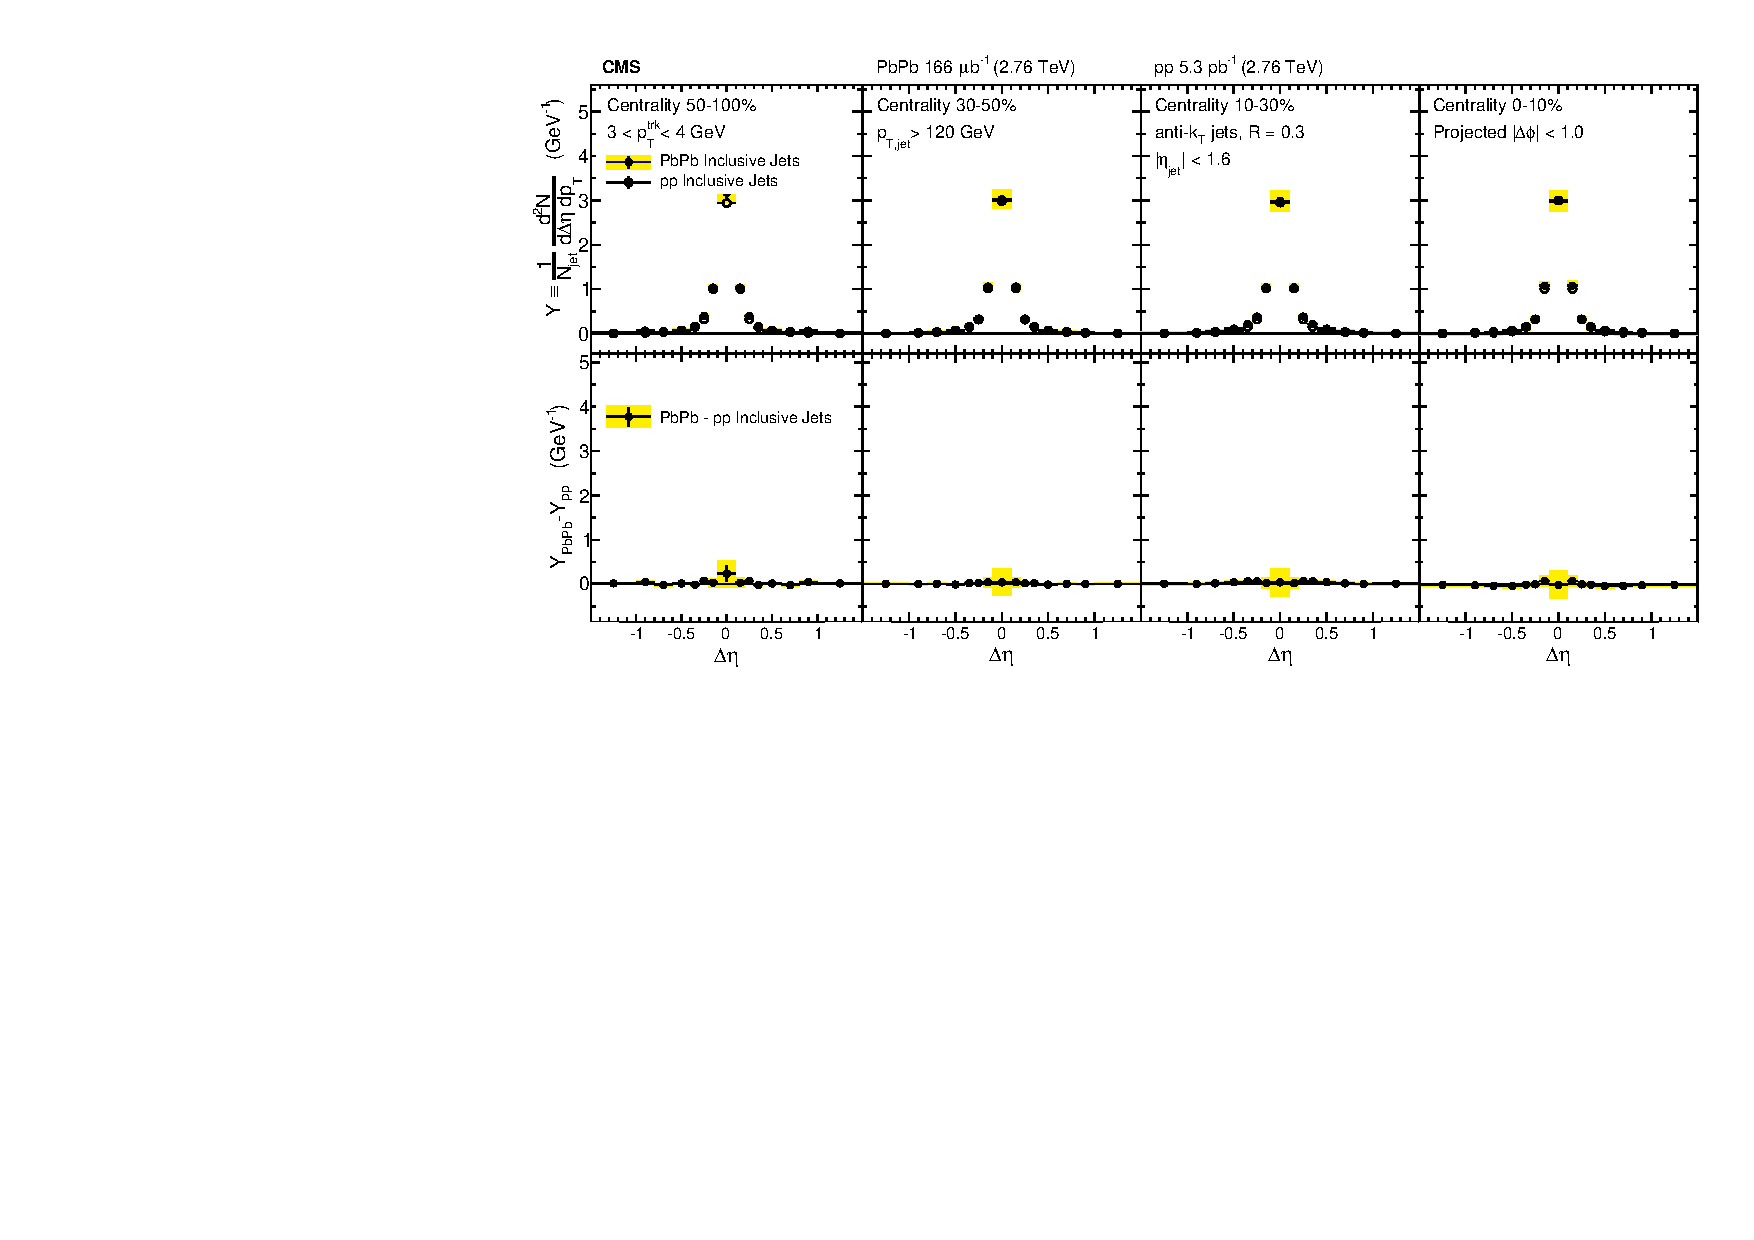
\includegraphics[width=0.99\textwidth]{figures/Results/PAS_Figure_3_TrkPt3_TrkPt4.pdf}
\caption[Inclusive jet $\Delta\eta$ correlations for tracks with $3 < p_{\rm T}^{\rm trk} < 4$ GeV at 2.76 TeV]{Symmetrized $\protect\Delta\eta$ distributions (projected over $|\Delta\phi| < 1$) of background-subtracted particle yields correlated to PbPb and pp inclusive jets with $p_{\rm T}>$ 120 GeV are shown in the top panels for tracks with 3 $ < p_{\rm T}^{\rm trk} < $ 4 GeV.  The difference in PbPb and pp per-jet yields is shown in the bottom panels. The total systematic uncertainties are shown as shaded boxes, and statistical uncertainties are shown as vertical bars (often smaller than the symbol size).}
\label{fig:Inclusive_dEta3}
\end{center} 
\end{figure} 

\begin{figure}[hbt] 
\begin{center} 
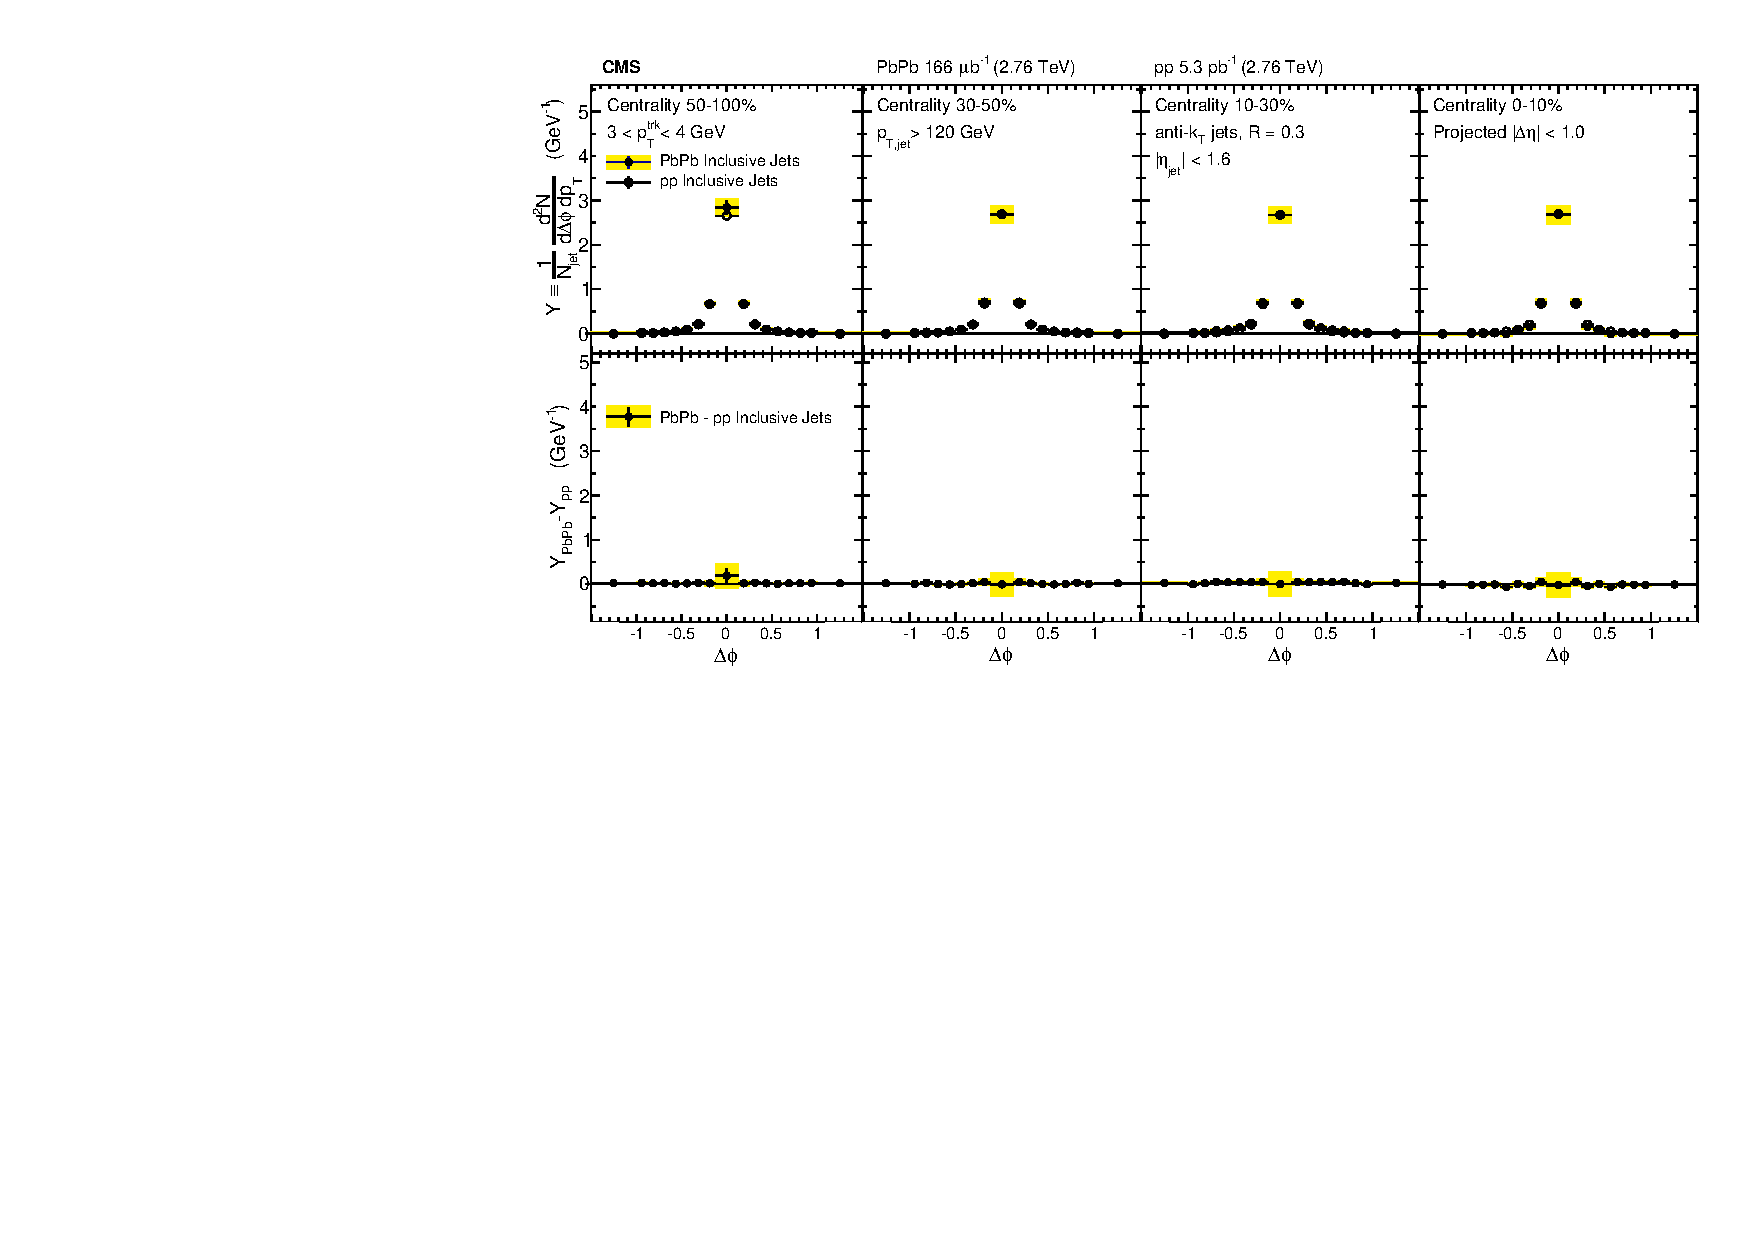
\includegraphics[width=0.99\textwidth]{figures/Results/PAS_Figure_4_TrkPt3_TrkPt4.pdf}
\caption[Inclusive jet $\Delta\phi$ correlations for tracks with $3 < p_{\rm T}^{\rm trk} < 4$ GeV at 2.76 TeV]{Symmetrized $\protect\Delta\phi$ distributions  (projected over $|\Delta\eta| < 1$) of background-subtracted particle yields correlated to PbPb and pp inclusive jets with $p_{\rm T} >$ 120 GeV are shown in the top panels for tracks with 3 $ < p_{\rm T}^{\rm trk} < $ 4 GeV.  The difference in PbPb and pp per-jet yields is shown in the bottom panels. The total systematic uncertainties are shown as shaded boxes, and statistical uncertainties are shown as vertical bars (often smaller than the symbol size).}
\label{fig:Inclusive_dPhi3} 
\end{center} 
\end{figure} 



\begin{figure}[hbt] 
\begin{center} 
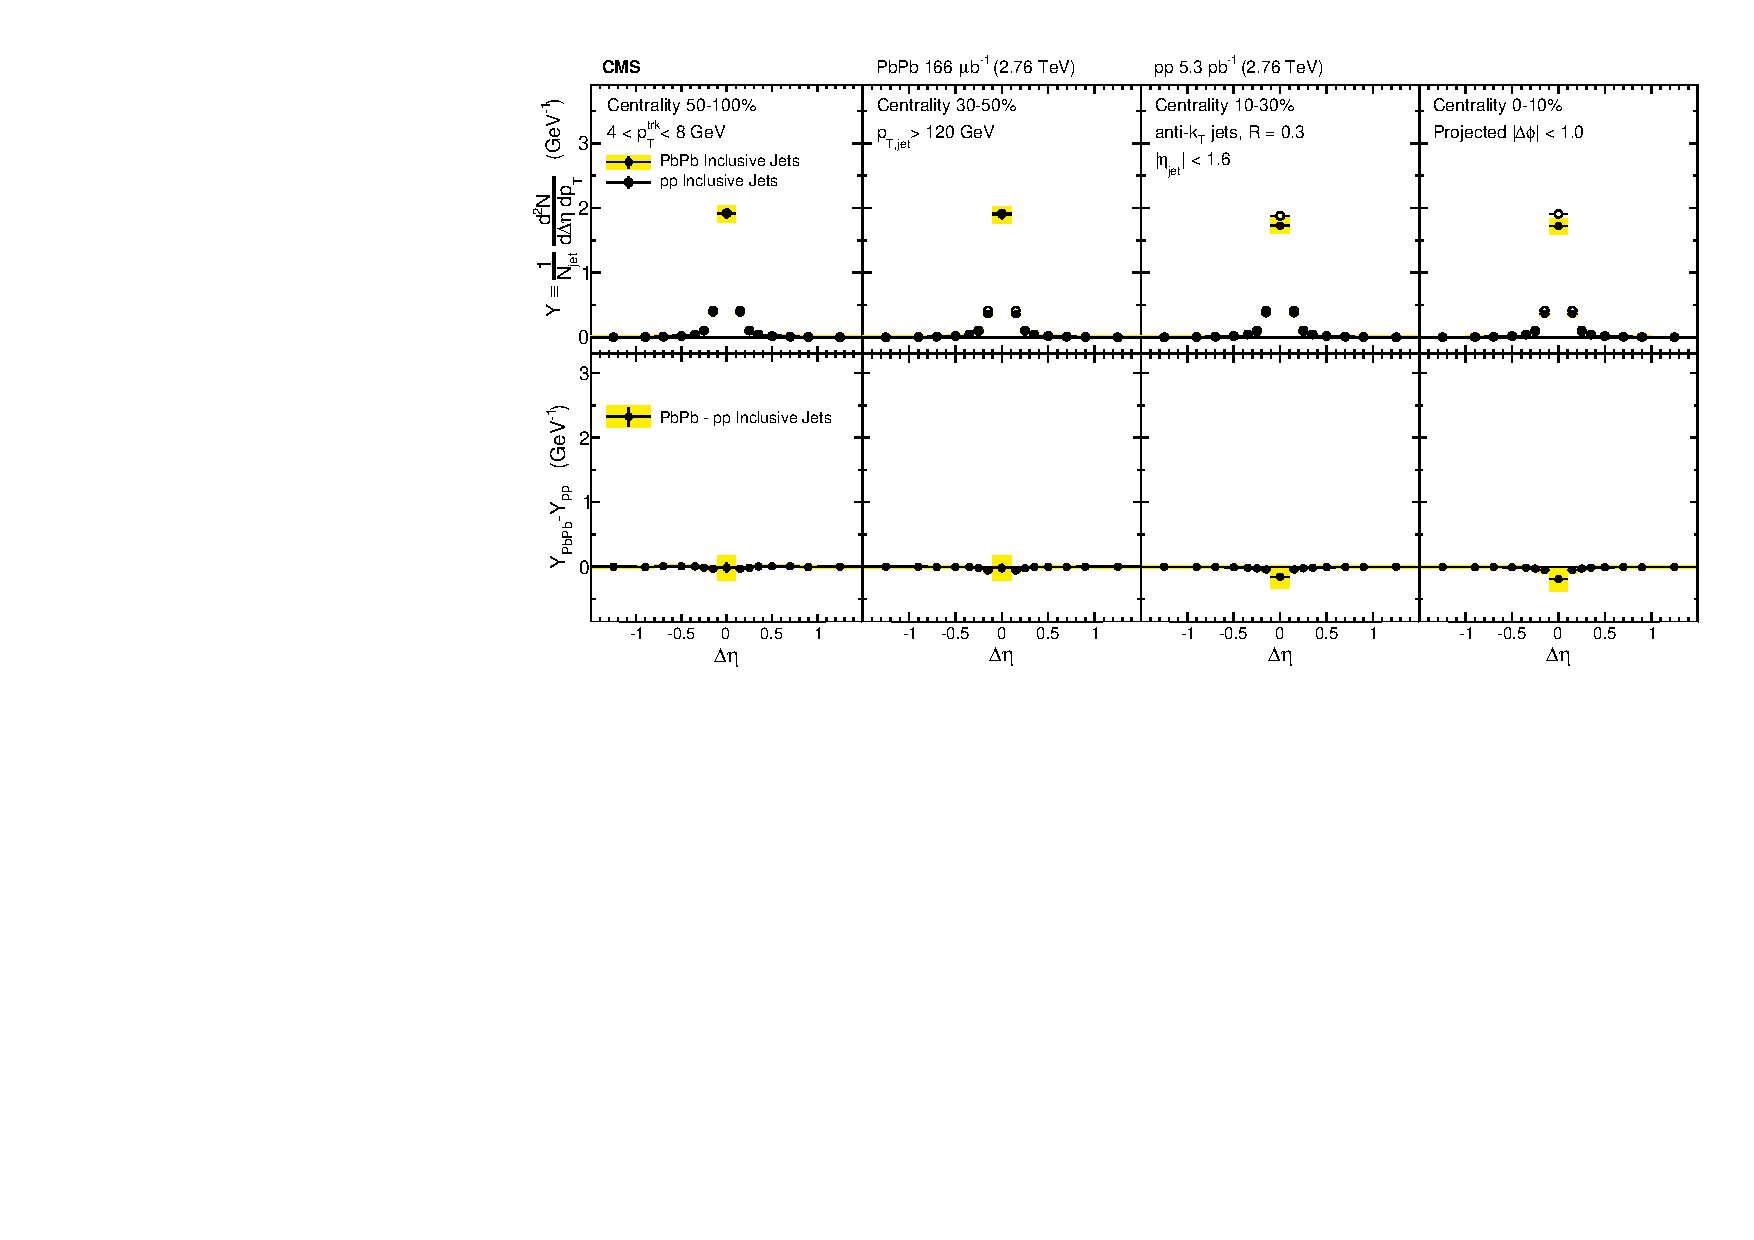
\includegraphics[width=0.99\textwidth]{figures/Results/PAS_Figure_3_TrkPt4_TrkPt8.pdf}
\caption[Inclusive jet $\Delta\eta$ correlations for tracks with $4 < p_{\rm T}^{\rm trk} < 8$ GeV at 2.76 TeV]{Symmetrized $\protect\Delta\eta$ distributions (projected over $|\Delta\phi| < 1$) of background-subtracted particle yields correlated to PbPb and pp inclusive jets with $p_{\rm T}>$ 120 GeV are shown in the top panels for tracks with 4 $ < p_{\rm T}^{\rm trk} < $ 8 GeV.  The difference in PbPb and pp per-jet yields is shown in the bottom panels. The total systematic uncertainties are shown as shaded boxes, and statistical uncertainties are shown as vertical bars (often smaller than the symbol size).}
\label{fig:Inclusive_dEta4}
\end{center} 
\end{figure} 

\begin{figure}[hbt] 
\begin{center} 
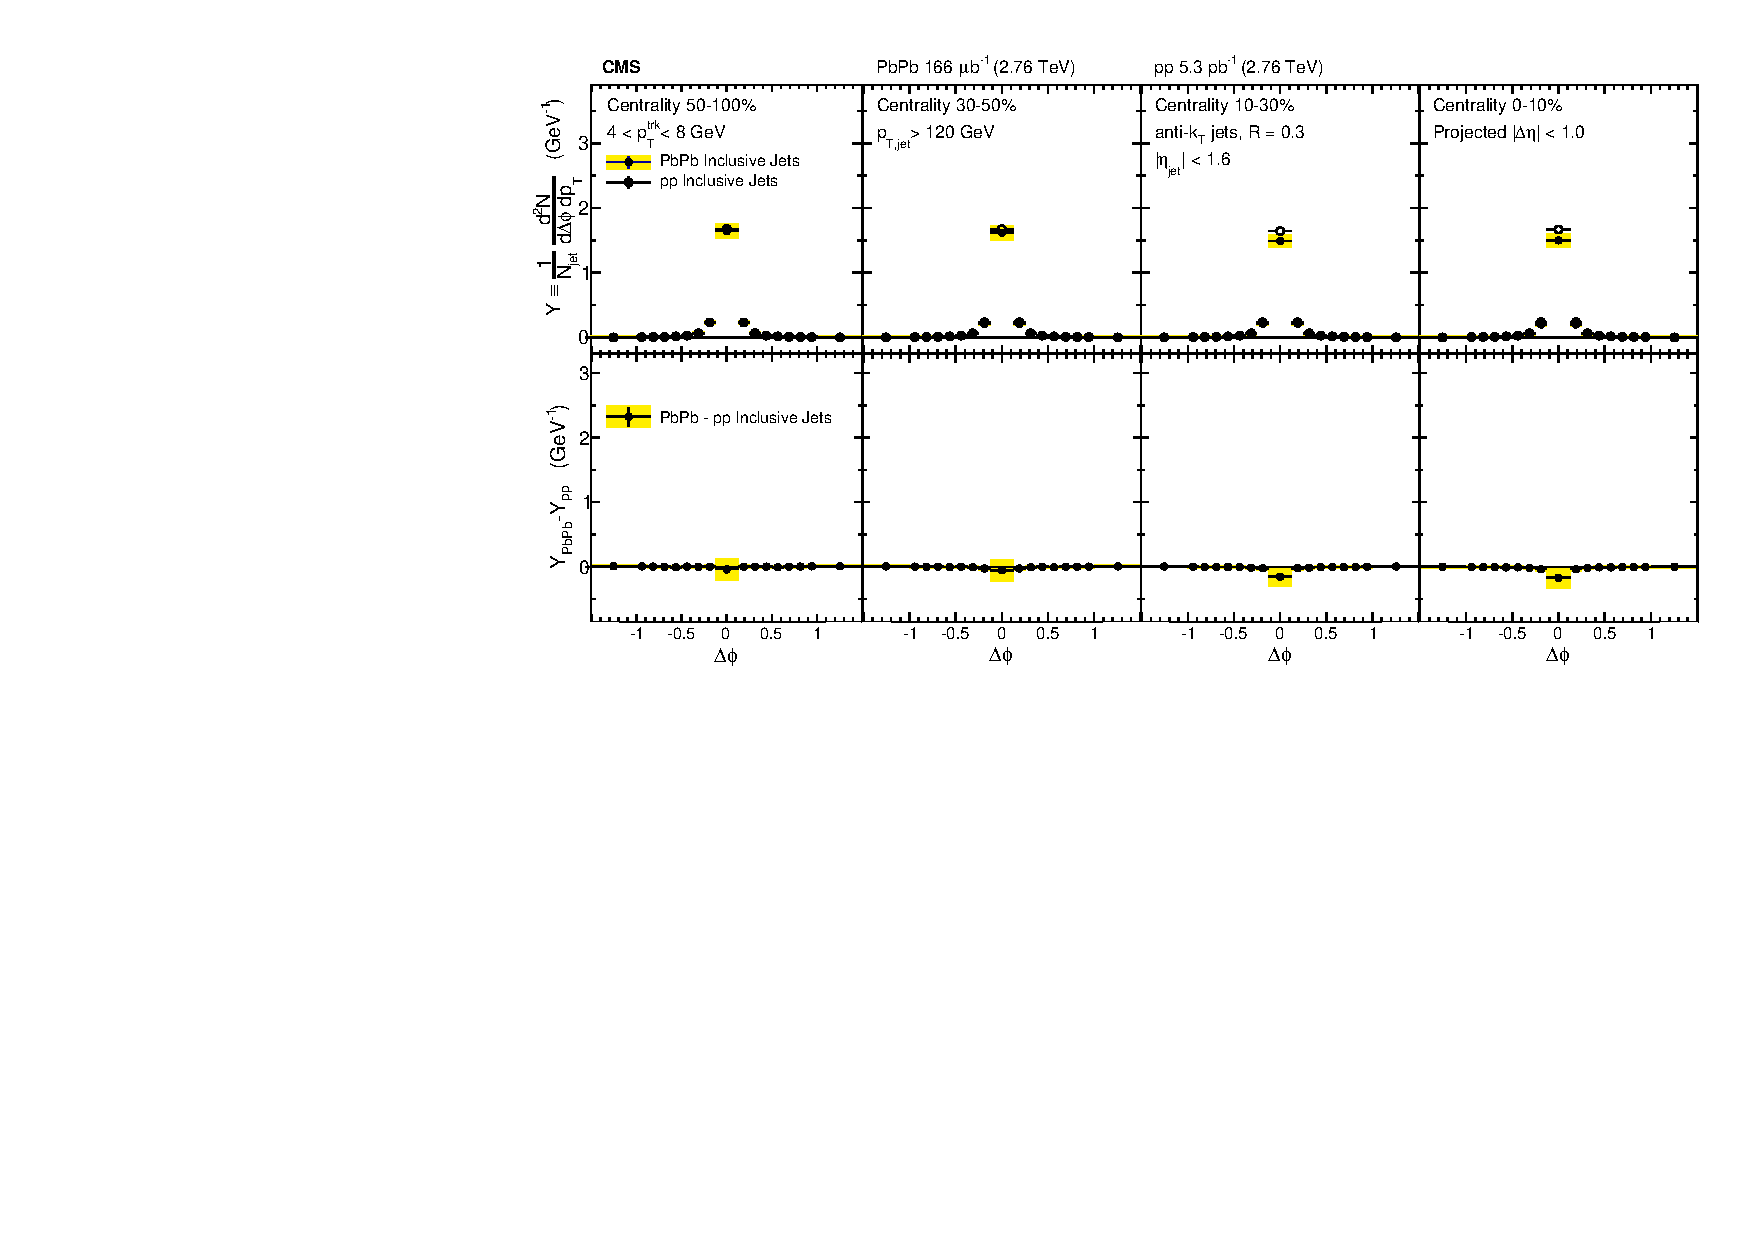
\includegraphics[width=0.99\textwidth]{figures/Results/PAS_Figure_4_TrkPt4_TrkPt8.pdf}
\caption[Inclusive jet $\Delta\phi$ correlations for tracks with $4 < p_{\rm T}^{\rm trk} < 8$ GeV at 2.76 TeV]{Symmetrized $\protect\Delta\phi$ distributions  (projected over $|\Delta\eta| < 1$) of background-subtracted particle yields correlated to PbPb and pp inclusive jets with $p_{\rm T} >$ 120 GeV are shown in the top panels for tracks with 4 $ < p_{\rm T}^{\rm trk} < $ 8 GeV.  The difference in PbPb and pp per-jet yields is shown in the bottom panels. The total systematic uncertainties are shown as shaded boxes, and statistical uncertainties are shown as vertical bars (often smaller than the symbol size).}
\label{fig:Inclusive_dPhi4} 
\end{center} 
\end{figure} 

 \begin{figure}[hbt]
    \begin{center}
       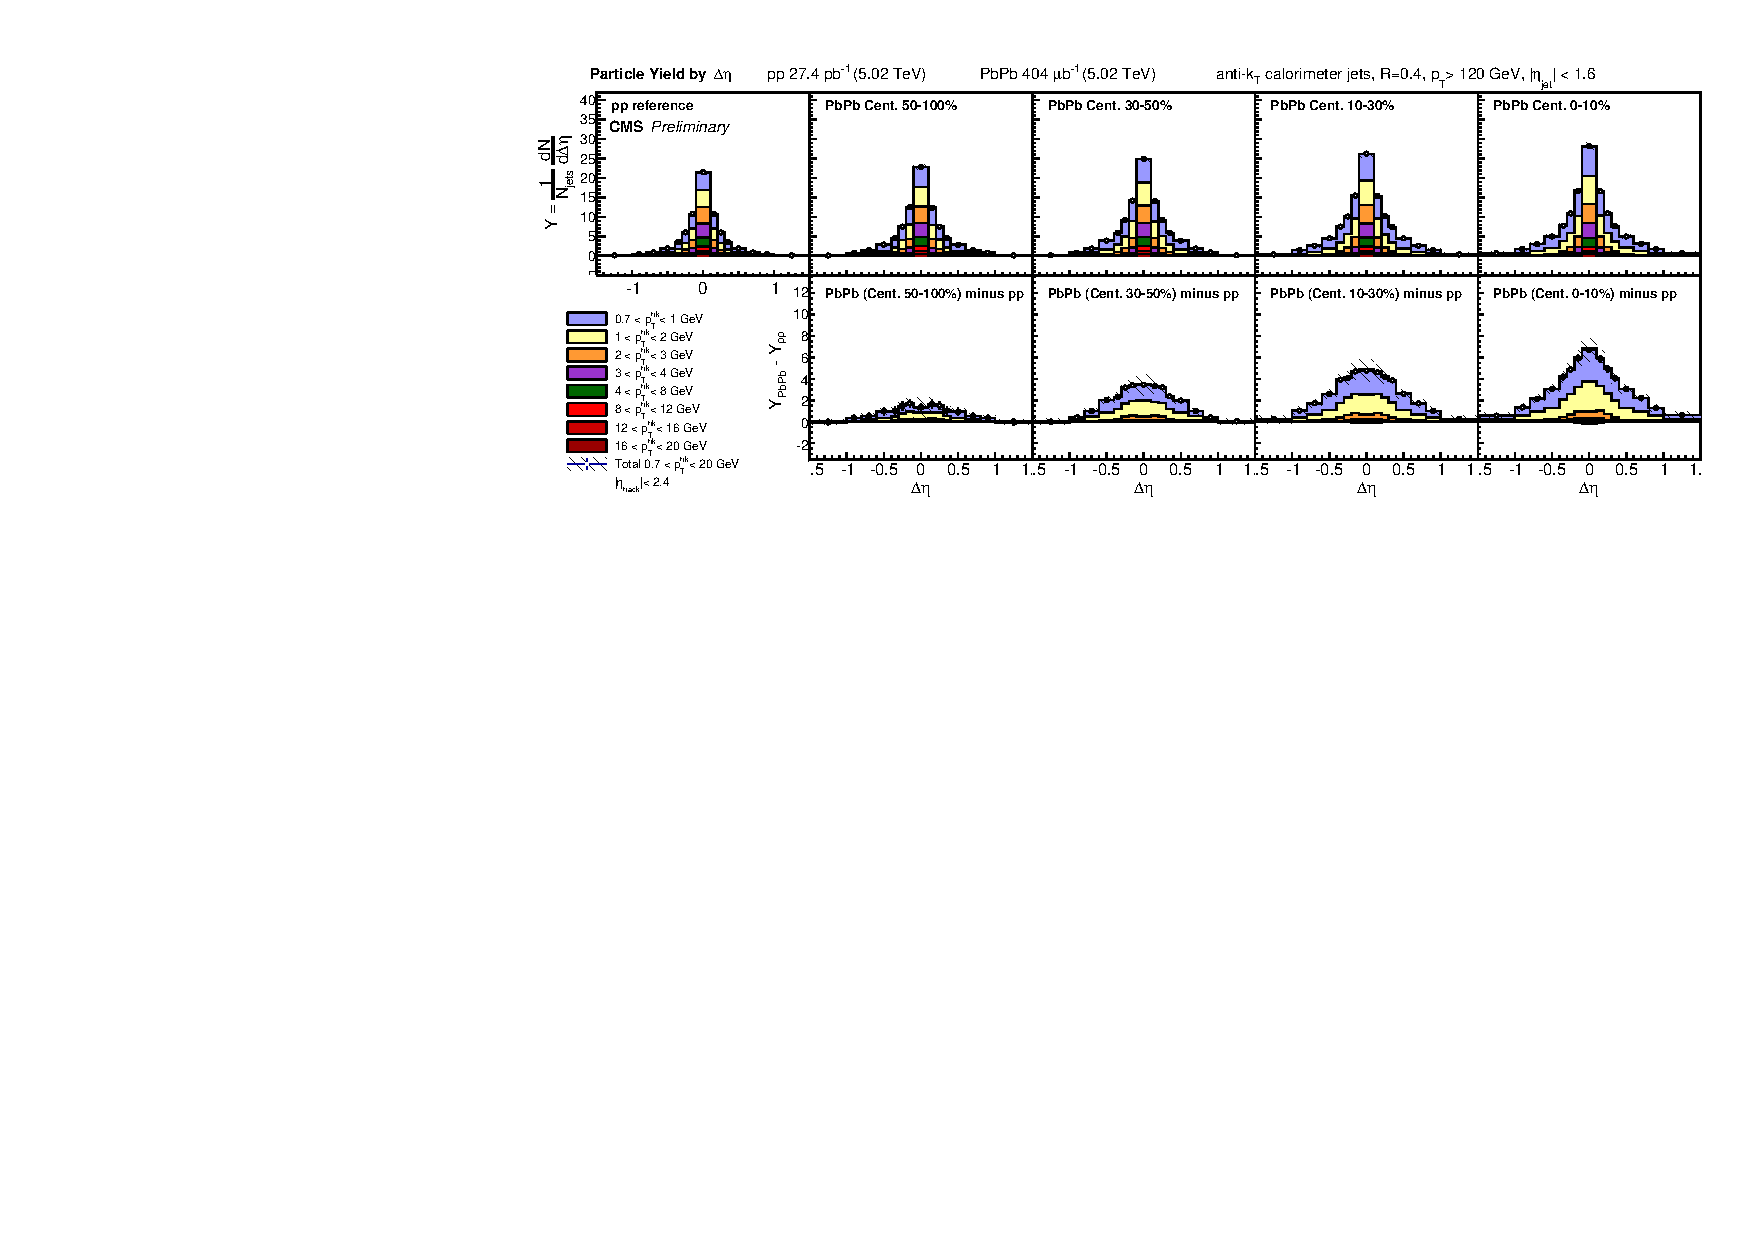
\includegraphics[width=0.99\textwidth]{figures/results/Yield_dEta_Stacked.pdf}
         \caption[Inclusive jet $\Delta\eta$ correlations at 5.02 TeV]{Top row: distributions of charged particle yields correlated to jets with $p_{\rm T} > 120$ GeV as a function of $\protect\Delta\eta$ (projected over $|\Delta\phi| < 1$), shown differentially for all $p_{\rm T}^{\rm trk}$ bins for pp, peripheral PbPb, and central PbPb data. Bottom row:  PbPb minus pp difference in these distributions.  Hatched lines on $p_{\rm T}^{\rm trk}$-inclusive points show total systematic uncertainties. }
       \label{fig:yield_deta_stacked}
    \end{center}
 \end{figure}
 
  \begin{figure}[hbt]
    \begin{center}
       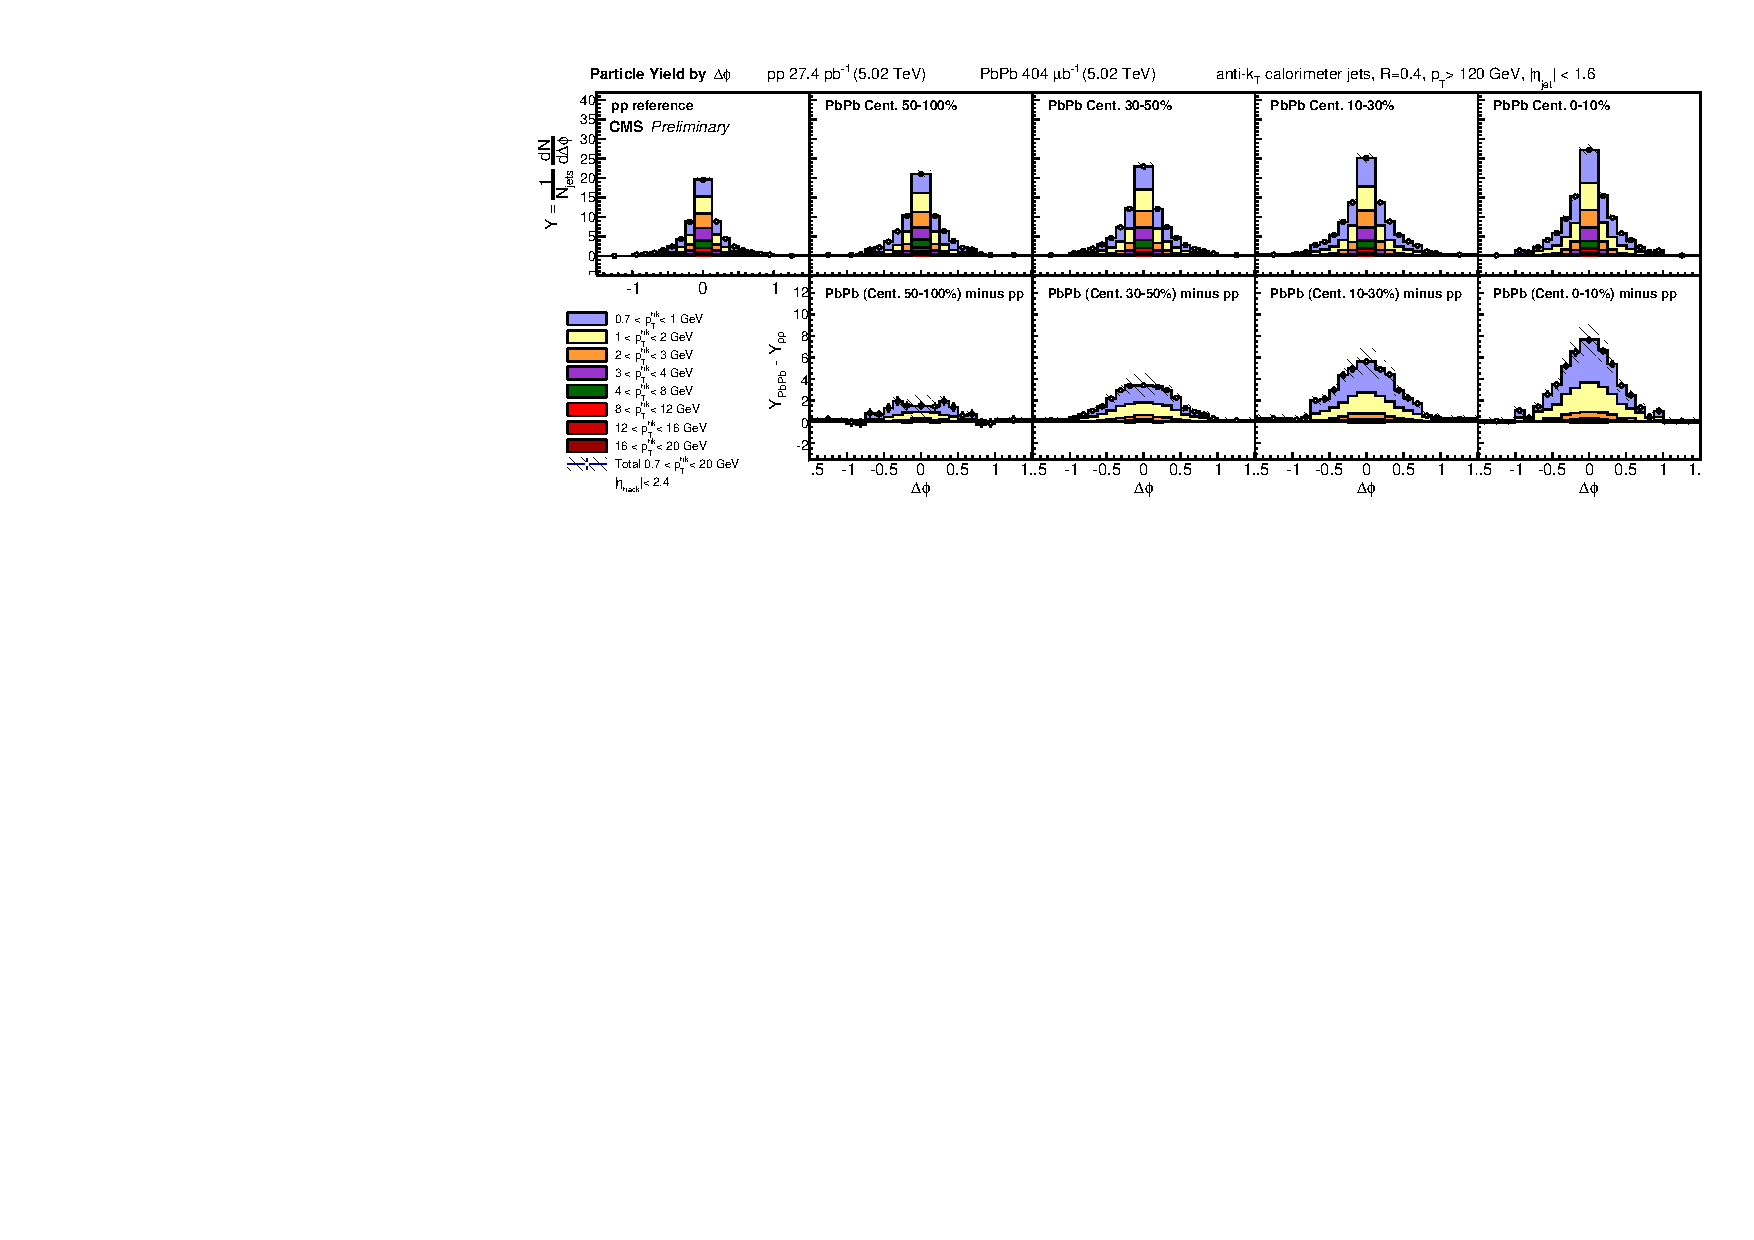
\includegraphics[width=0.99\textwidth]{figures/results/Yield_dPhi_Stacked.pdf}
         \caption[Inclusive jet $\Delta\phi$ correlations at 5.02 TeV]{Top row:  distributions of charged particle yields correlated to jets with $p_{\rm T} > 120$ GeV as a function of $\protect\Delta\phi$ (projected over $|\Delta\eta| < 1$), shown differentially for all $p_{\rm T}^{\rm trk}$ bins for pp, peripheral PbPb, and central PbPb data. Bottom row:  PbPb minus pp difference in these distributions.  Hatched lines on $p_{\rm T}^{\rm trk}$-inclusive points show total systematic uncertainties.}
       \label{fig:yield_dphi_stacked}
    \end{center}
 \end{figure}
 
  \begin{figure}[hbt]
    \begin{center}
       \includegraphics[width=0.99\textwidth]{figures/results/ParticleYield_by_dR.pdf}
         \caption[Inclusive jet distribution of charged particles as a function of $\Delta r$ at 5.02 TeV]{Top row:  distributions of charged particle yields correlated to jets with $p_{\rm T} > 120$ GeV as a function of $\protect\Delta r$, shown differentially for all $p_{\rm T}^{\rm trk}$ bins. Bottom row:  PbPb minus pp difference in these distributions. Hatched lines on $p_{\rm T}^{\rm trk}$-inclusive points show total systematic uncertainties.}
       \label{fig:yield_dr_stacked}
    \end{center}
 \end{figure}
 
 \clearpage
 
To summarize the magnitude of the modifications to particle yields in PbPb relative to pp colllisions, integrated yields as a function of $p_{\rm T}^{\rm trk}$ are presented in in the top panel of Fig.~\ref{fig:yield_integral}.  The bottom panel of Fig.~\ref{fig:yield_integral} shows differences PbPb--pp in total integrated particle yields in each $p_{\rm T}^{\rm trk}$ class for results at 5.02 TeV compared to 2.76 TeV results.  This quantifies the low-$p_{\rm T}$ excess in central PbPb collisions to as many as 4 additional particles (in central PbPb relative to pp reference) per unit of $p_{\rm T}^{\rm trk}$ in the lowest $p_{\rm T}^{\rm trk}$ bin.  This excess decreases smoothly with $p_{\rm T}^{\rm trk}$ in each centrality bin, until the 4--8 GeV central PbPb bin is consistent with or slightly depleted relative to pp reference.  For tracks with  $p_{\rm T}^{\rm trk} > 8 $ GeV, there is no evident modification in PbPb compared to pp.  Excess yields do not exhibit significant dependence on collision energies; particle yields at low-$p_{\rm T}^{\rm trk}$ are consistently larger at 5.02 TeV than at 2.76 TeV, but within the systematic uncertainties of the two measurements. 

 
  \begin{figure}[hbt]
    \begin{center}
       \includegraphics[width=0.99\textwidth]{figures/results/Integral_dR.pdf}
         \caption[Integrated inclusive jet charged particle yields at 2.76 and 5.02 TeV]{Top row: integrated yields of charged particle yields correlated to jets with $p_{\rm T} > 120$ GeV as a function of $p_{\rm T}^{\rm trk}$ bins for PbPb data, compared to pp reference.  Bottom row:  integrated excess yield, PbPb minus pp. New measurements of excess yields at 5.02 TeV are compared to those measured at 2.76 TeV.}       \label{fig:yield_integral}
    \end{center}
 \end{figure}


\clearpage

\subsection{Dijet correlation results at 2.76 TeV}
\label{sec:dijet_corr}

In the studies of charged-particle yields correlated to an inclusive sample of jets with $p_{\rm T} > 120$ GeV presented above, jet quenching is evident in the redistribution of $p_{\rm T}^{\rm trk}$ from harder to softer particles, and particularly in the observed centrality-dependent excess of low-$p_{\rm T}^{\rm trk}$ particle yields.  Jet quenching effects may be further probed by considering charged-particle yields correlated to each jet axis in dijet events.  Requiring events with two back-to-back jets (leading jet $p_{\rm T,1} > 120$ GeV, subleading jet $p_{\rm T,2} > 50$ GeV, $\Delta\phi_{\rm 1,2} > \frac{5\pi}{6}$), we construct separate correlations to the leading and the subleading jet axes.  In pp data, most dijets are balanced while in central PbPb a greater fraction of dijet pairs are unbalanced (as discussed in Sec.~\ref{sec:jet_sel}), suggesting that central PbPb data contains a significant fraction of dijet pairs in which the highest- and second-highest-$p_{\rm T}$ hard-scattering products had similar transverse momenta, but in which one jet experienced a greater path-length through the medium and correspondingly greater quenching.  This is expected to correspond to a ``surface-bias'' toward leading jets with very short path-lengths through the medium, that might be expected to cause minimal quenching in the leading jet sample.  It is therefore interesting to separately compare charged-particle distributions with respect to the leading and subleading jet axes in PbPb and pp data to look for evidence of path-length dependence in jet quenching.  

Figures~\ref{fig:fig2_dEta1} and~\ref{fig:fig2_dPhi1} show these correlation patterns in $\Delta\eta$ and $\Delta\phi$, respectively, for the $1 < p_{\rm T}^{\rm trk}$ GeV range in which the greatest quenching was evident in the 2.76 TeV inclusive jet studies.  As expected, quenching effects are greater for subleading than leading jets, as evident in larger excesses of soft particles in subleading jet correlations (while retaining the same centrality trends and gaussian-like distributions observed for the inclusive jet sample).  However, leading jets exhibit evidence of quenching as well, showing similar soft-particle excesses to those observed in the inclusive sample.  To quantitatively compare subleading and leading jet modifications to those in the inclusive jet sample, Fig.~\ref{fig:Excess_vs_trkpt} shows integrated particle yields for all three jet samples at 2.76 TeV.  Here it is clear that leading jets show similar PbPb--pp modifications to those observed in the inclusive sample, with approximately 2 excess particles in PbPb compared to pp data at lowest-$p_{\rm T}^{\rm trk}$, while the subleading jet sample shows as manty as 4 excess particles in PbPb compared to pp data at lowest-$p_{\rm T}^{\rm trk}$.

\begin{figure}[hbtp]
\begin{center}
\includegraphics[width=0.99\textwidth]{figures/Results/PAS_Figure_5_TrkPt1_TrkPt2.pdf}
\caption[Dijet $\Delta\eta$ correlations for tracks with $1 < p_{\rm T}^{\rm trk} < 2$ GeV at 2.76 TeV]{The top panels show the $\protect\Delta\eta$ distributions (projected over $|\Delta\phi| < 1$) of charged-particle background-subtracted yields correlated to PbPb and pp leading jets with $p_{\rm T, jet1}>$ 120~GeV.  The middle panels show the same distributions for subleading jets with $p_{\rm T, jet2}>$ 50~GeV, and the bottom panels show the difference PbPb minus pp for both leading and subleading jets. The total systematic uncertainties are shown as shaded boxes, and statistical uncertainties are shown as vertical bars (often smaller than the symbol size).}
 \label{fig:fig2_dEta1}
   \end{center}
\end{figure}

\begin{figure}[hbtp]
\begin{center}
\includegraphics[width=0.99\textwidth]{figures/Results/PAS_Figure_6_TrkPt1_TrkPt2.pdf}
     \caption[Dijet $\Delta\phi$ correlations for tracks with $1 < p_{\rm T}^{\rm trk} < 2$ GeV at 2.76 TeV]{The top panels show the $\protect\Delta\phi$ distributions (projected over $|\Delta\eta < 1$) of charged-particle background-subtracted yields correlated to PbPb and pp leading jets with $p_{\rm T, jet1}>$ 120~GeV.  The middle panels show the same distributions for subleading jets with $p_{\rm T, jet2}>$ 50~GeV, and the bottom panels show the difference PbPb minus pp for both leading and subleading jets. The total systematic uncertainties are shown as shaded boxes, and statistical uncertainties are shown as vertical bars (often smaller than the symbol size).}
      \label{fig:fig2_dPhi1}
   \end{center}
\end{figure}

\begin{figure}[hbtp]
\begin{center}
\includegraphics[width=0.99\textwidth]{figures/Results/PAS_Figure_7_WithInclusive.pdf}
\caption[Integrated charged particle yields for inclusive, leading, and subleading jets]{Total excess correlated yield observed in the PbPb data with respect to the reference measured in pp collisions, shown as a function of track $p_{\rm T}$ in four different centrality intervals (0--10\%, 10--30\%, 30--50\%, 50--100\%) for both leading jets with $p_{\rm T, jet1}> $120~GeV and subleading jets with $p_{\rm T, jet2}>$ 50~GeV. The total systematic uncertainties are shown as shaded boxes, and statistical uncertainties are shown as vertical bars (often smaller than the symbol size).}
\label{fig:Excess_vs_trkpt}
\end{center}
\end{figure}

\clearpage

In addition to characterizing the magnitude of jet quenching products (via the centrality-dependent excess of low-$p_{\rm T}^{trk}$ tracks greatest in correlations to subleading jets but also present in leading jet correlations), modifications to charged-particle correlated yields may also be characterized by their widths.  These studies are are relevant to look for the presence and extent of jet peak broadening due to medium interactions, and can be used to distinguish between different models for jet-medium interaction and medium-modified jet radiation.  In order to characterize correlation widths, correlations are fit to double-gaussian functions (all $\Delta\eta$ fits are shown in Appendix~\ref{app:width_determination} for illustration), and the width ($\sigma$) of these fits is obtained as the range in $|\Delta\eta|$ or $|\Delta\phi|$ containing 67\% of the total yield under the fit curve.   To obtain systematic uncertainties on these fits, points are varied up and down by their systematic uncertainties, and widths are re-calculated from these varied distributions.  

Figures~\ref{fig:Width_eta_lead} and~\ref{fig:Width_phi_lead} show correlation widths in $\Delta\eta$ and $\Delta\phi$ for leading jets in PbPb and pp data at 2.76 TeV.   At low-$p_{\rm T}^{\rm trk}$ there is a significant broadening evident in central PbPb data when compared to pp data, with this broadening decreasing in more peripheral collisions and with increasing $p_{\rm T}^{\rm trk}$ (with similar trends to those exhibited by correlated yield magnitudes).  Widths and width modifications are similar in $\Delta\eta$ and $\Delta\phi$, but slightly broader in $\Delta\phi$ for PbPb data.  These leading jet correlation widths and width modifications may also be compared to subleading jet correlation widths and width modifications, shown in Figs.~\ref{fig:Width_eta_sub} and~\ref{fig:Width_phi_sub}.  In peripheral PbPb data subleading and leading correlation widths are similar, but subleading jet PbPb correlation widths exhibiting less centrality dependence than leading jet correlation widths so that leading jet correlations in central PbPb data are slightly broader than than subleading jet correlations (but not significantly so, when taking into account the systematic uncertainties on both measurements).  Subleading jet peaks in pp data are, however, significantly broader than leading jet peaks in pp data--as is to be expected since the kinematic selection defining subleading jet as that with lower-$p_{\rm T}$, also implies that subleading jets will on average have softer fragmentation than leading jets.  Since subleading pp jets are broader than leading pp jets while subleading and leading jets have similar widths in PbPb, the jet peak broadening quantified as the PbPb--pp difference in widths is greater for leading jets than for subleading jets.  

\begin{figure}[hbtp]
\begin{center}
\includegraphics[width=0.99\textwidth]{figures/Results/Width_Eta_Leading.pdf}
\caption[Leading jet $\Delta\eta$ correlation widths as a function of $p_{\rm T}^{\rm trk}$ at 2.76 TeV]{Comparison of the widths in PbPb and pp of the $\protect\Delta\eta$ charged-particle distributions correlated to leading jets with $p_{\rm T, jet1}>$ 120~GeV, as a function of $p_{\rm T}^{\rm trk}$.  The bottom row shows the difference of the widths in PbPb and pp data.  The shaded band corresponds to systematic uncertainty, and statistical uncertainties are smaller than symbol size.}
\label{fig:Width_eta_lead}
\end{center}
\end{figure}

\begin{figure}[hbtp]
\begin{center}
\includegraphics[width=0.99\textwidth]{figures/Results/Width_Phi_Leading.pdf}
\caption[Leading jet $\Delta\phi$ correlation widths as a function of $p_{\rm T}^{\rm trk}$ at 2.76 TeV]{Comparison of the widths in PbPb and pp of the $\protect\Delta\phi$ charged-particle distributions correlated to leading jets with $p_{\rm T, jet1}>$ 120~GeV, as a function of $p_{\rm T}^{\rm trk}$.  The bottom row shows the difference of the widths in PbPb and pp data.  The shaded band corresponds to systematic uncertainty, and statistical uncertainties are smaller than symbol size.}
\label{fig:Width_phi_lead}
\end{center}
\end{figure}

\begin{figure}[hbtp]
\begin{center}
\includegraphics[width=0.99\textwidth]{figures/Results/Width_Eta_SubLeading.pdf}
\caption[Subleading jet $\Delta\eta$ correlation widths as a function of $p_{\rm T}^{\rm trk}$ at 2.76 TeV]{Comparison of the widths in PbPb and pp of the $\protect\Delta\eta$ charged-particle distributions correlated to leading jets with $p_{\rm T, jet2}>$ 50~GeV, as a function of $p_{\rm T}^{\rm trk}$.  The bottom row shows the difference of the widths in PbPb and pp data.  The shaded band corresponds to systematic uncertainty, and statistical uncertainties are smaller than symbol size.}
\label{fig:Width_eta_sub}
\end{center}
\end{figure}

\begin{figure}[hbtp]
\begin{center}
\includegraphics[width=0.99\textwidth]{figures/Results/Width_Phi_SubLeading.pdf}
\caption[Subleading jet $\Delta\phi$ correlation widths as a function of $p_{\rm T}^{\rm trk}$ at 2.76 TeV]{Comparison of the widths in PbPb and pp of the $\protect\Delta\phi$ charged-particle distributions correlated to leading jets with $p_{\rm T, jet2}>$ 50~GeV, as a function of $p_{\rm T}^{\rm trk}$.  The bottom row shows the difference of the widths in PbPb and pp data.  The shaded band corresponds to systematic uncertainty, and statistical uncertainties are smaller than symbol size.}
\label{fig:Width_phi_sub}
\end{center}
\end{figure}



\clearpage


\subsection{Jet shapes at 2.76 TeV and 5.02 TeV}
\label{sec:jet_shapes}

A common observable to characterize and compare the widths of jet peaks is the jet shape $\rho_{\Delta r}$, measuring the fraction of total jet transverse momentum as a function of distance $\Delta r$ from the jet axis.  As discussed in Sec.~\ref{sec:theory_models}, previous CMS measurements of jet shape~\cite{Chatrchyan:2013kwa} have gained particular attention from the theoretical community in efforts to constrain models of jet energy loss.  Jet shape measurements to large angles ($\Delta r = 1$, compared to previous measurements to only $\Delta r = 0.3$) may be obtained from correlation studies, extending measurements to the full range of the jet peak and offering the capability of distinguishing between theoretical predictions based on earlier, more narrow, measurements.  

In the correlation technique, jet shapes are obtained by weighting correlations by $p_{\rm T}^{\rm trk}$, and integrating the resulting (background-subtracted) 2D jet-peak momentum distributions in annuli with radial width $\protect\Delta r = 0.05$, where each has an inner radius of ${\rm r_{a}} = \Delta r - \delta r/2$ and an outer radius of ${\rm r_{b}} = \Delta r + \delta r/2$.  For this measurement, an inclusive high-$p_{\rm T}^{\rm trk}$ bin is included to capture particles with $20 < p_{\rm T}^{\rm trk}< 300 $ GeV.   The resulting transverse momentum profile of the jet is defined as: 

\begin{equation}
{\rm P} (\Delta r) = \frac{1}{\delta r} \frac{1}{N_{\rm jets}} \large{\Sigma_{\rm jets}} \Sigma_{\rm tracks \in (r_{a},r_{b})} p_{\rm T}^{\rm trk}
\end{equation}

\noindent This profile is then normalized to unity within $\protect\Delta r = 1$ to produce the jet shape $\rho(\Delta r)$: 

\begin{equation}
\rho(\Delta r) = \frac{1}{\delta r} \frac{\large{\Sigma_{\rm jets}} \Sigma_{\rm tracks \in (r_{a},r_{b})} p_{\rm T}^{\rm trk}}{\large{\Sigma_{\rm jets}} \Sigma_{\rm tracks} p_{\rm T}^{\rm trk}}
\end{equation}


The top row of Fig.~\ref{fig:jetshape_dr_stacked} presents the inclusive jet transverse momentum profile ${\rm P}(\Delta r)$ in pp and PbPb data at 5.02 TeV, while the middle row shows the jet shape ${\rho}(\Delta r)$, normalized to unity within $\protect\Delta r = 1$.  Here again redistribution of energy from small to large angles from the jet cone is evident in PbPb relative to pp reference, as seen in the dipping then rising trend in the jet shape ratio $\rho(\Delta r)_{\rm PbPb}/\rho(\Delta r)_{\rm pp}$ presented in the bottom row.  

\clearpage

  \begin{figure}[hbt]
    \begin{center}
       \includegraphics[width=0.99\textwidth]{figures/results/JetShapes_WithHighpT_pTweighted_3Row.pdf}
         \caption[Inclusive jet shape at 5.02 TeV, shown differentially in $p_{\rm T}^{\rm trk}$]{Top row: Transverse momentum profile of inclusive jets ${\rm P}(\Delta r)$ in pp and PbPb data at 5.02 TeV, shown differentially in $p_{\rm T}^{\rm trk}$.  Middle row: jet shapes $\rho(\Delta r)$ (normalized to unity over $\protect\Delta r < 1$) in PbPb and pp. Bottom row:  jet shape ratio $\rho(\Delta r)_{\rm PbPb} / \rho(\Delta r)_{\rm pp}$. Hatched lines on $p_{\rm T}^{\rm trk}$-inclusive points show total systematic uncertainties.}
       \label{fig:jetshape_dr_stacked}
    \end{center}
 \end{figure}


In addition to studies of inclusive jet shapes, it is also interesting to consider the jet shapes and jet shape modifications of leading and subleading jets in dijet events.  These studies are carried out with the same selection of 2.76 TeV dijet events used for the correlation studies presented in~\ref{sec:dijet_corr}.  In this case, for consistency with a previous CMS study measured the jet shape $\rho(\Delta r)$ within the jet cone radius $\Delta r = 0.3$~\cite{Chatrchyan:2013kwa} at 2.76 TeV, these leading and subleading jet shape measurements at 2.76 TeV are normalized to integrate to unity with in the radius $\Delta r < 0.3$.  In Fig.~\ref{fig:JetShape_Leading}, the leading jet shape measured with this correlation technique is compared to the published CMS reference and extend this measurement to $\Delta r = 1$, noting that the leading jet shape is consistent within uncertainties with the previous measurement for an inclusive jet selection of all jets with $p_{\rm T}>100$ GeV.  A new measurement of subleading jet shape in Fig.~\ref{fig:JetShape_SubLeading} is then presented.  As noted in the correlation width measurements discussed in Sec.~\ref{sec:dijet_corr}, subleading jets in pp data are broader than leading jets in pp data.  Therefore, although the PbPb-to-pp $modifications$ are similar for leading and subleading jets, the more steeply falling pp leading jet shape results in a greater \textit{relative} modification shown in the jet shape ratio $\rho_{\rm PbPb}(\Delta r)/\rho_{\rm pp}(\Delta r)$ for leading than for subleading jets.  Similarly, when comparing jet shape measurements at 2.76 TeV to those at 5.02 TeV, it is relevant to note hat the pp reference is broader at 5.02 TeV than at 2.76 TeV, likely due to the greater fraction of gluon versus quark jets that pass the kinematic selections of the analysis at the higher center-of-mass energy.  


\begin{figure}[h!]
\begin{center} 
\includegraphics[width=0.99\textwidth]{figures/Results/JetShapes_WithHighpT_PAS.pdf}
\caption[Leading jet shape at 2.76 TeV, shown differentially in $p_{\rm T}^{\rm trk}$]{Top row:  leading jet shape $\rho(\Delta r)$ for pp reference and central and peripheral PbPb data, shown for all tracks with $p_{\rm T}^{\rm trk} > 0.5$ GeV and decomposed by track transverse momentum.  Shapes are normalized to unity over the region $r<0.3$ for consistency with the published reference shown (Ref.~\cite{Chatrchyan:2013kwa}).  Bottom row:  leading jet shape ratio $\rho(\Delta r)_{\rm PbPb}/\rho(\Delta r)_{\rm pp}$, again with published reference.  }
\label{fig:JetShape_Leading} 
\end{center} 
\end{figure} 



\begin{figure}[h!]
\begin{center} 
\includegraphics[width=0.99\textwidth]{figures/Results/JetShapes_SubLeading_WithHighpT_PAS.pdf}
\caption[Subleading jet shape at 2.76 TeV, shown differentially in $p_{\rm T}^{\rm trk}$]{Top row:  subleading jet shape $\rho(\Delta r)$ for pp reference and central and peripheral PbPb data, shown for all tracks with $p_{\rm T}> 0.5$ GeV and decomposed by track transverse momentum, normalized to unity over the region $\Delta r<0.3$ Bottom row:  subleading jet shape ratio $\rho(\Delta r)_{\rm PbPb}/\rho(\Delta r)_{\rm pp}$. }
\label{fig:JetShape_SubLeading} 
\end{center} 
\end{figure} 



\clearpage



\subsection{Decomposition of hemisphere momentum balance in dijet events at 2.76 TeV}
\label{sec:dijet_mpt}

The dijet results at 2.76 TeV presented in this analysis are complimented by other CMS measurements conducted on the same data using the ``missing-$p_{\rm T}$'' hemisphere momentum balance method presneted in Ref.~\cite{HIN_2014_010} and discussed in Secs.~\ref{sec:theory_jets} and~\ref{sec:theory_models}.  In this analysis, a ``dijet'' axis is constructed by averaging the leading jet and subleading jet axes (these are separated by $\Delta\phi_{\rm 1,2} = \pi$ on average, but are not necessarily parallel in each event due to 3-jet events) to construct a dijet axis, dividing the event into leading and subleading hemispheres with respect to this axis, and comparing the hemisphere-wide distributions of $p_{\rm T}^{\rm trk}$ (projected, in this case, onto the combined dijet axis) to obtain the subleading-to-leading balancing distribution as a function of distance from the dijet axis $\Delta r$.  The jet track correlation technique may be used to obtain this same measurement (comparing subleading-to-leading distributions on average rather than event-by-event, and making use of the fact that the subleading and leading jet axes are \textit{on average} perfectly back-to-back).  When this cross-check is performed \textit{without background subtraction}, the two techniques yield consistent results, despite methodological differences and differences in jet-$\eta$ cuts.  This hemisphere-wide missing-$p_{\rm T}$ technique is also used to extract differences in total particle yields between the leading and subleading hemispheres, and shows an average excess of 4-5 particles with $p_{\rm T}^{\rm trk}$ in the subleading hemisphere compared to the leading hemisphere~\cite{HIN_2014_010}.  In the dijet correlation studies presented in this analysis \textit{with background subtraction}, however, only approximately 2 additional particles were found correlated to the subleading jet peak compared to the leading jet peak, as shown in Sec.~\ref{sec:dijet_corr}.  This apparent difference motivates a detailed examination and decomposition of the distribution of $p_{\rm T}^{\rm trk}$ in dijet events in order to consider contributions to the hemisphere-wide momentum balance from both the leading and subleading jet peaks, and from the long-range correlated underlying event.  

For this investigation, the dijet samples of 2.76 TeV PbPb and pp data are each divided based on asymmetry paramter $A_{\rm J}$ to further illuminate quenching effects and to decompose the contributions to the hemisphere $p_{\rm T}^{\rm trk}$ balance studied in Ref.~~\cite{HIN_2014_010}:  a balanced sample with $A_{\rm J} < 0.22$, and an ``unbalanced'' sample with $A_{\rm J} > 0.22$.  Transverse momenum distributions for each sample are constructed in $\Delta\eta--\Delta\phi$ for each sample, and are corrected for pair-acceptance effects.  Like all particle density and $p_{\rm T}^{\rm trk}$ correlations studied in this analysis, these show jet peaks on an underlying event that shows significant $\Delta\phi$ correlations but is flat in $\Delta\eta$.  Correlations are therefore projected into $\Delta\phi$ for further study in order to preserve this underlying event structure.  Studies will begin by considering the hemisphere-wide ``missing-$p_{\rm T}$'' distribution as a function of $\Delta\phi$, and will then decompose this distribution into jet peak and underlying event contributions, and finally consider the relative contributions from jet peaks and from the underlying event to the overall hemisphere $p_{\rm T}^{\rm trk}$ balance for balanced and unbalanced dijets.   

Figures~\ref{fig:MpT_nobkgsub_Aj0_Aj22} and~\ref{fig:MpT_nobkgsub_Aj22_Aj75} present the hemisphere-wide balancing distribution of transverse momentum around the subleading versus the leading jet for balanced and unbalanced dijets respectively.  For both selections, a wide excess of soft particles in the subleading versus leading hemisphere in central PbPb collisions relative to pp reference is evident, reflecting the greater quenching of the subleading jet.  In the unbalanced selection, as required by momentum conservation, the signal is enhanced in both pp and PbPb data:  in pp a large excess of particles with $p_{\rm T}>3$ GeV long-range is present on the subleading side, compensating for the lower momentum of the highest-$p_{\rm T}$ particles in the jet itself.  In peripheral PbPb data the distribution is quite similar to pp reference, while in central PbPb data this balancing distribution consists mostly of soft particles $p_{\rm T}<3$ GeV, consistent with the findings of a previous CMS study~\cite{HIN_2014_010}.  To better demonstrate these medium modifications, the difference in yield between PbPb and pp collisions is shown in the bottom panels of Fig.~\ref{fig:MpT_nobkgsub_Aj0_Aj22} and Fig.~\ref{fig:MpT_nobkgsub_Aj22_Aj75}.

\begin{figure}[h!]
\begin{center} 
\includegraphics[width=0.99\textwidth]{figures/Results/Missing_pT_NoBkgSub_Aj0_Aj22.pdf}
\caption[Dijet subleading-to-leading hemisphere momentum balance for balanced dijets]{Top row:  total hemisphere distribution in $\protect\Delta\phi$ of excess tranverse momentum about the subleading relative to the leading jet for balanced dijets with $A_{\rm J} < 0.22$, shown differentially by track transverse momentum for pp reference, peripheral PbPb, and central PbPb data.  Bottom row:  PbPb--pp difference in these $\protect\Delta\phi$ momentum distributions.}
\label{fig:MpT_nobkgsub_Aj0_Aj22} 
\end{center} 
\end{figure} 

\begin{figure}[hbt]
\begin{center} 
\includegraphics[width=0.99\textwidth]{figures/Results/Missing_pT_NoBkgSub_Aj22_Aj75.pdf}
\caption[Dijet subleading-to-leading hemisphere momentum balance for unbalanced dijets]{Top row:  total hemisphere distribution in $\protect\Delta\phi$ of excess tranverse momentum about the subleading relative to the leading jet for balanced dijets with $A_{\rm J} > 0.22$, shown differentially by track transverse momentum for pp reference, peripheral PbPb, and central PbPb data.  Bottom row:  PbPb--pp difference in these $\protect\Delta\phi$ momentum distributions.}
\label{fig:MpT_nobkgsub_Aj22_Aj75} 
\end{center} 
\end{figure} 

To better understand the redistribution of transverse momentum within the QGP, the distributions are then separated into three components as discussed above:  the gaussian-like peaks about the leading and subleading jet axes, plus a component accounting for overall subleading-to-leading asymmetry in the $\protect\Delta\phi$-correlated long-range underlying event (measured in the region $1.5<|\Delta\eta|<2.5$.  In Fig.~\ref{fig:MpT_jetrelated_Aj0_Aj22} and Fig.~\ref{fig:MpT_jetrelated_Aj22_Aj75}, the jet peak components are shown for balanced and unbalanced jets respectively, presenting subleading results positive and leading results negative (in line with the hemisphere difference measurements in Fig.~\ref{fig:MpT_nobkgsub_Aj22_Aj75} and Fig.~\ref{fig:MpT_nobkgsub_Aj0_Aj22}).  Jet peak distributions after decomposition are projected over the full range $|\Delta\eta|<2.5$, again for consistency with the hemisphere difference measurements.  The top row of each panel first shows the overall distribution of momentum carried by particles with $p_{\rm T} < 8$ GeV on about the jet peak.  The middle two panels then assess modifications to the subleading and leading jets, respectively.  Here there is evidence of quenching to both the subleading and the leading jet in central PbPb collisions relative to pp reference, with an excess of low-$p_{\rm T}^{\rm trk}$ particles correlated to the jet axis in both the balanced and unbalanced dijet selections, as observed in the charged particle density studies presented in Sec.~\ref{sec:dijet_corr}.  In unbalanced dijets this enhancement of soft-$p_{\rm T}^{\rm trk}$ particles turns into a depletion at higher-$p_{\rm T}^{\rm trk}$, and is greater on the subleading than the leading side.  To compare between hemispheres and assess the jet peak contribution to the overall hemisphere momentum balance, the double difference PbPb--pp, subleading--leading is presented in the bottom panel.  Here it is evident that the low-$p_{\rm T}^{\rm trk}$ excess in central PbPb collisions is larger on the subleading than the leading side of the dijet system, but larger subleading-to-leading excess only accounts for only a portion of the total momentum redistribution in unbalanced dijet events.

\begin{figure}[hbt]
\begin{center} 
\includegraphics[width=0.99\textwidth]{figures/Results/Missing_pT_JetRelated_Aj0_Aj22.pdf}
\caption[Jet peak subleading-to-leading momentum balance for balanced dijets]{Top row:  jet-peak (long-range subtracted) distribution in $\protect\Delta\phi$ of tranverse momentum about the subleading (plotted positive) and leading (plotted negative) jets for balanced dijets with $A_{\rm J} < 0.22$.  Middle rows:  PbPb--pp momentum distribution differences for subleading and leading jets.  Bottom row:  PbPb--pp, subleading--leading double difference in these $\protect\Delta\phi$ momentum distributions.}
\label{fig:MpT_jetrelated_Aj0_Aj22} 
\end{center} 
\end{figure} 

\begin{figure}[hbt]
\begin{center} 
\includegraphics[width=0.99\textwidth]{figures/Results/Missing_pT_JetRelated_Aj22_Aj75.pdf}
\caption[Jet peak subleading-to-leading momentum balance for unbalanced dijets]{Top row:  jet-peak (long-range subtracted) distribution in $\protect\Delta\phi$ of tranverse momentum about the subleading (plotted positive) and leading (plotted negative) jets for balanced dijets with $A_{\rm J} > 0.22$.  Middle rows:  PbPb--pp momentum distribution differences for subleading and leading jets.  Bottom row:  PbPb--pp, subleading--leading double difference in these $\protect\Delta\phi$ momentum distributions.}
\label{fig:MpT_jetrelated_Aj22_Aj75} 
\end{center} 
\end{figure} 

\clearpage

These jet-related studies are complemented by an analysis of the long-range subleading to leading asymmetry, presented in Fig.~\ref{fig:MpT_longrange_Aj0_Aj22}  and Fig.~\ref{fig:MpT_longrange_Aj22_Aj75} for balanced and unbalanced jets respectively.  The long-range correlated background in balanced dijet events is symmetric in pp and peripheral PbPb data, while in central PbPb data there is a small excess of low-$p_{\rm T}^{\rm trk}$ particles.  In unbalanced dijets, however, there is significant asymmetry already in pp reference, with a large correlated excess of particles in all $p_{\rm T}$ classes less than 8 GeV on the subleading relative to leading side of the underlying event.  This asymmetry reflects the presence of other hard-scattering products in the subleading hemisphere dijet event, as required by momentum conservation when selecting asymmetric dijets in vacuum-like collisions.  In the presence of the strongly interacting medium;  however, this underlying event asymmetry in asymmetric dijet events changes notably.  In peripheral PbPb collisions there is already some depletion of momentum carried by high-$p_{\rm T}^{\rm trk}$ particles, and in central pp collisions subleading-to-leading underlying event excesses with $p_{\rm T}^{\rm trk} > 2$ GeV vanish nearly completely.  To assess the contribution of this long-range asymmetry to the total hemisphere imbalance, the double difference PbPb--pp, subleading--leading is plotted on the bottom panel as for (and on the same scale as) the double difference shown for the jet peaks.  To assess the overall hemisphere momentum balance attributed to this long-range asymmetry, the hemisphere integral ($|\Delta\phi|<\pi/2$ and $|\Delta\eta|<2.5$) is presented in Fig.~\ref{fig:Integral_Longrange} for balanced versus unbalanced dijets.  For unbalanced dijets, the the overall asymmetry rises with track-$p_{\rm T}$ pp reference, but falls with track-$p_{\rm T}$ for central PbPb data.  

\begin{figure}[hbt]
\begin{center} 
\includegraphics[width=0.99\textwidth]{figures/Results/Missing_pT_LongRange_Aj0_Aj22.pdf}
\caption[long-range subleading-to-leading momentum balance for balanced dijets]{Top row:  long-range distribution in $\protect\Delta\phi$ of excess tranverse momentum in the subleading relative to leading sides for balanced dijets with $A_{\rm J} < 0.22$.  Bottom row:  PbPb--pp difference in these $\protect\Delta\phi$ long-range momentum distributions.}
\label{fig:MpT_longrange_Aj0_Aj22} 
\end{center} 
\end{figure} 

\begin{figure}[hbt]
\begin{center} 
\includegraphics[width=0.99\textwidth]{figures/Results/Missing_pT_LongRange_Aj22_Aj75.pdf}
\caption[long-range subleading-to-leading momentum balance for unbalanced dijets]{Top row:  long-range distribution in $\protect\Delta\phi$ of excess tranverse momentum in the subleading relative to leading sides for balanced dijets with $A_{\rm J} > 0.22$.  Bottom row:  PbPb--pp difference in these $\protect\Delta\phi$ long-range momentum distributions.}
\label{fig:MpT_longrange_Aj22_Aj75} 
\end{center} 
\end{figure} 


\begin{figure}[h!]
\begin{center} 
\includegraphics[width=0.99\textwidth]{figures/Results/Integral_Longrange.pdf}
\caption[Integrated transverse momentum in the long-range $\protect\Delta\phi$-correlated distribution as a function of track-$p_{\rm T}$]{Integrated transverse momentum in the long-range $\protect\Delta\phi$-correlated distribution as a function of track-$p_{\rm T}$ integrated over $|\Delta\phi| < \pi/2$  and $|\Delta\phi| < 2.5$ and for pp reference, peripheral PbPb and central PbPb data for balanced compared to unbalanced dijets.}
\label{fig:Integral_Longrange} 
\end{center} 
\end{figure} 


Finally, to show the relative conributions to overall hemisphere momentum balance from the leading and subleading jet peaks as well as from the long-range underlying event asymmetry, a summary of hemisphere-integrated excess (PbPb--pp) yield for balanced and unbalanced dijets in central PbPb collisions is shown in Fig.~\ref{fig:Integral_Summary} and Fig.~\ref{fig:Integral_Summary_Peripheral} for central and peripheral collisions respectively.  The top panels of Fig.~\ref{fig:Integral_Summary} present total PbPb minus pp differences in transvese momentum associated with the subleading jet (plotted positive) and leading jet (plotted negative).  Modifications to the distribution of tracks with $p_{\rm T}< 3$ GeV are evident for both the leading and subleading jet peaks, with a greater enhancement of low-$p_{\rm T}^{\rm trk}$ particles associated with the subleading jet.   These total jet peak modifications in central PbPb collisions are not significantly different in unbalanced versus balanced dijets.  The bottom panels of Fig.~\ref{fig:Integral_Summary} present these jet-peak modifications together with the long-range modifications evident in Fig.~\ref{fig:Integral_Longrange} to show the decomposed hemisphere-wide differences in associated transverse momentum in each $p_{\rm T}^{\rm trk}$ range.  Unlike the jet peak contributions, the long-range PbPb versus modifications differ outsie of uncertainties between balanced and unbalanced dijets:  here the depletion of high-$p_{\rm T}^{\rm trk}$ particles in unbalanced PbPb versus pp dijets corresponds to the reduced contribution from third jets (which are prominently evident in the long-range distribution for pp unbalanced dijet events) in central PbPb unbalanced dijet events.  Figure~\ref{fig:Integral_Summary_Peripheral} presents the same hemisphere-integrated PbPb minus pp excess information for peripheral collisions for comparison to the central results shown in Fig.~\ref{fig:Integral_Summary}.  Some possible small modifications are already evident in this 50-100\% centrality range, but these differences between peripheral PbPb and pp results are in most cases smaller than systematic uncertainties.


\begin{figure}[hbt]
\begin{center} 
\includegraphics[width=0.99\textwidth]{figures/Results/Integral_PbPb_pp_Summary.pdf}
\caption[Relative contributions from jet peaks and long-range asymmetry to the double difference PbPb--pp, subleading--leading in total hemisphere transverse momentum for central collisions]{Modifications of jet-hadron correlated transverse momentum in central PbPb collisions with respect to pp reference, integrated $|\Delta\phi| < \pi/2$, $|\Delta\phi| < 2.5$.  Top row:  subleading and leading jet peak PbPb--pp.  Bottom row:  relative contributions from jet peaks and long-range asymmetry to the double difference PbPb--pp, subleading--leading in total hemisphere transverse momentum. }
\label{fig:Integral_Summary} 
\end{center} 
\end{figure} 


\begin{figure}[hbt]
\begin{center} 
\includegraphics[width=0.99\textwidth]{figures/Results/Integral_PbPb_pp_Summary_Peripheral.pdf}
\caption[Relative contributions from jet peaks and long-range asymmetry to the double difference PbPb--pp, subleading--leading in total hemisphere transverse momentum for peripheral collisions]{Modifications of jet-hadron correlated transverse momentum in peripheral PbPb collisions with respect to pp reference, integrated $|\Delta\phi| < \pi/2$, $|\Delta\phi| < 2.5$.  Top row:  subleading and leading jet peak PbPb--pp.  Bottom row:  relative contributions from jet peaks and long-range asymmetry to the double difference PbPb--pp, subleading--leading in total hemisphere transverse momentum. }
\label{fig:Integral_Summary_Peripheral} 
\end{center} 
\end{figure} 


The decomposition of integrated jet peak and long-range correlated $p_{\rm T}^{\rm trk}$ shown in Fig.~\ref{fig:Integral_Summary} and Fig.~\ref{fig:Integral_Summary_Peripheral} clarify the relationship between the jet peak correlation studies presented in this analysis and the missing-$p_{\rm T}$ measurements presented in Ref.~\cite{HIN_2014_010}:  as shown through this detailed decomposition, comparing hemisphere distributions as a whole include contributions from the subleading and leading jet peaks studied in correlation studies, but also a contribution from the underlying event.  In both PbPb and pp data, the underlying event partially cancels with hemisphere subtraction:  contributions from combinatoric background and even flow harmonics ($V_{2}$ etc.) will cancel, while contributions from 3rd jets and and odd flow harmonics ($V_{1}$, $V_{3}$ etc.) will not.  As we have seen, in pp the non-cancelling underlying event is dominated by 3rd jets, especially in the unbalanced dijet selection in which their presence is kinematically required.  In PbPb (where the contribution from 3rd jet events is smaller), this underlying event has evident contributions from odd flow harmonics as well, reflecting coupling of jets to the event reaction plane.  

\clearpage


\subsection{Theory implications of these results}


https://arxiv.org/abs/1707.01539


\clearpage

\section{Conclusion}
\label{sec:Conclusion}
\input{Conclusion}
\clearpage

\bibliographystyle{unsrt}
\addcontentsline{toc}{section}{References}
\bibliography{HT_Thesis}

\clearpage


\appendix

\appendix
\section*{Appendices}
\addcontentsline{toc}{section}{Appendices}
\renewcommand{\thesubsection}{\Alph{subsection}}


\subsection{Jet kinematics}

The following sections summarize jet kinematics for inclusive jets and dijets at 2.76 TeV, for inclusive jets at 5.02 TeV, and for dijets in each asymmetry class at 2.76 TeV.

\subsubsection{Jet kinematics at 2.76 TeV}
\label{app:kinematics_run1}

The kinematic observables of jets in pp and PbPb 2.76 TeV events (solid markers) are compared with Monte Carlo (hatched marks). All spectra have been normalized to unity. Comparing the jet spectra observed in PbPb data (pp data) and in {\sc pythia+hydjet} ({\sc pythia}) samples, a reasonable agreement in the overall shape is found.
 
 
 \begin{figure}[h!]
 \begin{center}
 \includegraphics[width=.75\textwidth]{figures/Appendices/JetSpectra_MC_Data_Pythia_RecoJet_JetEtaCut16.pdf}
 \caption{Distribution of transverse momentum, pseudorapidity, and azimuthal distribution of all jet selections for Pythia data compared to {\sc pythia} simulation.}
  \label{fig:ppJetPt}
 \end{center}
 \end{figure}
 

 
  \begin{figure}[h!]
 \begin{center}
 \includegraphics[width=1\textwidth]{figures/Appendices/JetSpectra_MC_Data_HydJet_RecoJet_JetEtaCut16.pdf}
 \caption{Transverse momentum distribution of all jet selections for PbPb data  at 2.76 TeV compared to {\sc pythia+hydjet} simulation.}
 \label{fig:PbPbJetPt}
 \end{center}
 \end{figure}


 \begin{figure}[h!]
 \begin{center}
 \includegraphics[width=1\textwidth]{figures/Appendices/JetEta_MC_Data_HydJet_RecoJet_JetEtaCut16.pdf}
 \caption{ Pseudorapidity distribution of all jet selections for PbPb data at 2.76 TeV compared to {\sc pythia+hydjet} simulation.}
  \label{fig:PbPbJetEta}
 \end{center}
 \end{figure}
 
 
 \begin{figure}[h!]
 \begin{center}
 \includegraphics[width=1\textwidth]{figures/Appendices/JetPhi_MC_Data_HydJet_RecoJet_JetEtaCut16.pdf}
 \caption{Azimuthal angle distribution of all jet selections for PbPb data at 2.76 TeV compared to {\sc pythia+hydjet} simulation for each collision centrality bin.}
  \label{fig:PbPbJetPhi}
 \end{center}
 \end{figure}
 

 \clearpage
 
 
 
\subsubsection{Inclusive jet kinematics at 5.02 TeV}
\label{app:kinematics_run2}



Jet $p_{\rm T}$, $\eta$, and $\phi$ distributions for 5.02 TeV data, comparing PbPb data to {\sc pythia+hydjet} and pp data to {\sc pythia} simulation. 


 \begin{figure}[h!]
 \begin{center}

  \includegraphics[width=.75\textwidth]{figures/Appendices/JetKinematics_pp_Pythia.pdf}
 \caption{ Distribution of pseudorapidity distribution of all jet selections for PbPb data compared to {\sc pythia+hydjet} simulation for each collision centrality bin.}
\label{fig:ppJetPt2}
 \end{center}
 \end{figure}
 
 
  \begin{figure}[h!]
 \begin{center}
 \includegraphics[width=1\textwidth]{figures/Appendices/JetKinematics_PbPb_Hydjet.pdf}
 \caption{Transverse momentum distribution for PbPb data compared to {\sc pythia+hydjet} simulation for each collision centrality bin.}
 \label{fig:PbPbJetPt2} 
 \end{center}
 \end{figure}

  \begin{figure}[h!]
 \begin{center}
 \includegraphics[width=1\textwidth]{figures/Appendices/JetEta_PbPb_Hydjet.pdf}
 \caption{Jet $\eta$ distribution for PbPb data compared to {\sc pythia+hydjet} simulation for each collision centrality bin.}
 \label{fig:PbPbJetEta2} 
 \end{center}
 \end{figure}

 
  \begin{figure}[h!]
 \begin{center}
 \includegraphics[width=1\textwidth]{figures/Appendices/JetPhi_PbPb_Hydjet.pdf}
 \caption{Jet $\phi$ distribution for PbPb data compared to {\sc pythia+hydjet} simulation for each collision centrality bin.}
 \label{fig:PbPbJetPhi2} 
 \end{center}
 \end{figure}

  
 \subsubsection{Dijet kinematics in asymmetry classes at 2.76 TeV}

In the figures below, jet transverse momentum, pseudorapidity, and azimuth are shown for our Aj-inclusive sample, compared to each Aj selection in our analysis.  Note that $A_{\rm J}$-selection primarily affects the subleading jet spectrum, while the leading jet spectrum is nearly unchanged.  Jet $\eta$ and jet $\phi$ exhibit no significant $A_{\rm J}$-dependence for leading or subleading jets.  Distributions are shown first for pp, and then for PbPb data at 2.76 TeV.








\begin{figure}[htbp]
\begin{center}
\includegraphics[width=0.99\textwidth]{figures/Appendices/JetSummary_pp_Aj0_Aj11.pdf}
\caption{
Jet $p_{\rm T}$, $\eta$, and $\phi$ for all  pp dijets and for  pp dijets with $A_{\rm J}$:  $0<A_{\rm J}<0.11$.  
}
\label{fig:JetKin ppAj0Aj11}
\end{center}
\end{figure}

\begin{figure}[htbp]
\begin{center}
\includegraphics[width=0.99\textwidth]{figures/Appendices/JetSummary_pp_Aj11_Aj22.pdf}
\caption{
Jet $p_{\rm T}$, $\eta$, and $\phi$ for all  pp dijets and for  pp dijets with $A_{\rm J}$:  $0.11<A_{\rm J}<0.22$.  
}
\label{fig:JetKin ppAj11Aj22}
\end{center}
\end{figure}

\begin{figure}[htbp]
\begin{center}
\includegraphics[width=0.99\textwidth]{figures/Appendices/JetSummary_pp_Aj22_Aj33.pdf}
\caption{
Jet $p_{\rm T}$, $\eta$, and $\phi$ for all  pp dijets and for  pp dijets with $A_{\rm J}$:  $0.22<A_{\rm J}<0.33$.  
}
\label{fig:JetKin ppAj22Aj33}
\end{center}
\end{figure}


\begin{figure}[htbp]
\begin{center}
\includegraphics[width=0.99\textwidth]{figures/Appendices/JetSummary_pp_Aj33_Aj75.pdf}
\caption{
Jet $p_{\rm T}$, $\eta$, and $\phi$ for all  pp dijets and for  pp dijets with $A_{\rm J}$:  $A_{\rm J}>0.33$.  
}
\label{fig:JetKinppAj33Aj75}
\end{center}
\end{figure}


\begin{figure}[htbp]
\begin{center}
\includegraphics[width=0.99\textwidth]{figures/Appendices/JetSummary_PbPb_Aj0_Aj11.pdf}
\caption{Jet $p_{\rm T}$, $\eta$, and $\phi$ for all PbPb dijets and for PbPb dijets with  $0<A_{\rm J}<0.11$.  
}
\label{fig:JetKinPbPbAj0Aj11}
\end{center}
\end{figure}

\begin{figure}[htbp]
\begin{center}
\includegraphics[width=0.99\textwidth]{figures/Appendices/JetSummary_PbPb_Aj11_Aj22.pdf}
\caption{
Jet $p_{\rm T}$, $\eta$, and $\phi$ for all PbPb dijets and for PbPb dijets with $0.11<A_{\rm J}<0.22$.  
}
\label{fig:JetKinPbPbAj11Aj22}
\end{center}
\end{figure}

\begin{figure}[htbp]
\begin{center}
\includegraphics[width=0.99\textwidth]{figures/Appendices/JetSummary_PbPb_Aj22_Aj33.pdf}
\caption{
Jet $p_{\rm T}$, $\eta$, and $\phi$ for all PbPb dijets and for PbPb dijets with $0.22<A_{\rm J}<0.33$.  
}
\label{fig:JetKinPbPbAj22Aj33}
\end{center}
\end{figure}


\begin{figure}[htbp]
\begin{center}
\includegraphics[width=0.99\textwidth]{figures/Appendices/JetSummary_PbPb_Aj33_Aj75.pdf}
\caption{
Jet $p_{\rm T}$, $\eta$, and $\phi$ for all PbPb dijets and for PbPb dijets with $A_{\rm J}>0.33$.  
}
\label{fig:JetKinPbPbAj33Aj75}
\end{center}
\end{figure}


\clearpage




\subsection{Background fitting details}

\label{app:bkg_fits}

Figures~\ref{fig:dijet_fit}-\ref{fig:inc_fit} show the two steps of fits involved in modeling the the background distribution in $\Delta\phi$, as discussed in section~\ref{sec:bkg_sub}.

\begin{figure}[h!]
\begin{center}
\includegraphics[width=0.9\textwidth]{figures/Appendices/DijetFreeFitsGluedBackgroundV1V2V3.pdf}
\caption[Dijet background fits (preliminary step)]{Dijet combined background $\Delta\phi$ distributions, estimated by projection over the region 1.5$<|\Delta\eta|<$3.0.  Here the ''near-side'' region $\frac{-\pi}{2}<\Delta\phi<\frac{\pi}{2}$ is taken from the leading jet correlation, while the ''away-side'' $\frac{-\pi}{2}<\Delta\phi<\frac{\pi}{2}$ is taken from the subleading jet correlation.  The resulting combined background distribution is fit with the function $B^{dijet}(\Delta\phi) = B_{0}(1+2\rm{V}_{1}$Cos($\Delta\phi$)+$2\rm{V}_{2}$Cos(2$\Delta\phi$))+$2\rm{V}_{3}$Cos(3$\Delta\phi$)).}
\label{fig:dijet_fit}
\end{center}
\end{figure}


\begin{figure}[hbtp]
\begin{center}
\includegraphics[width=0.9\textwidth]{figures/Appendices/Fits_PbPb_Leading.pdf}
\caption[Leading jet background fits]{Background leading jet $\Delta\phi$ distributions, estimated by projection over the region 1.5$<|\Delta\eta|<$3.0, is fit as shown.  The 2D background distripbution is estimated by propagating the black fit line in $\Delta\eta$, with uncertainty assigned by varying fit parameters by the appropriate fit error as shown in the blue error band.}
\end{center}
\end{figure}


\begin{figure}[hbtp]
\begin{center}
\includegraphics[width=0.9\textwidth]{figures/Appendices/Fits_PbPb_SubLeading.pdf}
\caption[Subleading jet background fits]{Background subleading jet $\Delta\phi$ distributions, estimated by projection over the region 1.5$<|\Delta\eta|<$3.0, is fit as shown.  The 2D background distribution is estimated by propagating the black fit line in $\Delta\eta$, with uncertainty assigned by varying fit parameters by the appropriate fit error as shown in the blue error band.}
\end{center}
\end{figure}

\begin{figure}[h!]
\begin{center}
\includegraphics[width=0.9\textwidth]{figures/Appendices/Fits_PbPb_Inclusive.pdf}
\caption[Inclusive jet background fits]{Background inclusive jet $\Delta\phi$ distributions, estimated by projection over the region 1.5$<|\Delta\eta|<$3.0, is fit as shown.  The 2D background distribution is estimated by propagating the black fit line in $\Delta\eta$, with uncertainty assigned by varying fit parameters by the appropriate fit error as shown in the blue error band.}
\label{fig:inc_fit}
\end{center}
\end{figure}

\clearpage



\subsection{Pair acceptance and event decomposition systematic uncertainties}

\label{app:err_me_bkg}


Figure~\ref{fig:me_err} illustrates the estimation of pair-acceptance uncertainty, determined by considering the sideband asymmetry in the $\Delta\eta$ distributions of background subtracted yield.  

\begin{figure}[h!]
\begin{center}
\includegraphics[width=0.9\textwidth]{figures/Appendices/Eta_EdgeFit_PbPb_Inclusive.pdf}
\caption[Pair acceptance uncertainty determination]{Background-subtracted inclusive jet $\Delta\eta$ distribution is shown for sideband region 1.5$<|\Delta\eta|<$3.0 only.  Each side is fit separately with a horizontal line, and the greater deviation from zero is assigned as systematic uncertainty arising from the pair-acceptance correction.}
\label{fig:me_err}
\end{center}
\end{figure}

\clearpage


\noindent Figure~\ref{fig:bkg_err} illustrates the background-subtraction systematic uncertainty estimation:  the average content of the two 1.5$<\Delta\eta<$2.0 bins is assigned as systematic uncertainty for each $p_{\rm T}$ and centrality bin.  

\begin{figure}[h!]
\begin{center}
\includegraphics[width=0.9\textwidth]{figures/Appendices/Yield_Eta_wide_PbPb_Inclusive.pdf}
\caption[Background subtraction uncertainty determination]{Inclusive jet correlated yield in $\Delta\eta$, shown to axis range $|\Delta\eta|<2.0$.  The deviation of the most peripheral points from zero is assigned as systematic uncertainty as discussed in the Systematic Uncertainty section above.}
\label{fig:bkg_err}
\end{center}
\end{figure}
\clearpage



\subsection{Correlation widths and related uncertainty}

\label{app:width_determination}

\begin{figure}[h!]
\begin{center}

\includegraphics[width=0.9\textwidth]{figures/Appendices/Width_Check_Fits_Eta_PbPb_Leading.png}

\caption[Width determination for PbPb leading jets]{Illustration of the fits used to determine the distribution widths (shown here for leading jet PbPb $\Delta\eta$ correlations).  Correlations are fit to a double gaussian (shown in blue, with black dashed lines indicating constituent gaussians), and width is taken as the $\Delta\eta$ value containing 67\% of the total yield. Points are varied by their systematic errors and the fits are repeated (shown in red) to obtain the systematic error on the width.}
\label{fig:Width_check_fit_PbPb_lead}
\end{center}
\end{figure}



\begin{figure}[hbtp]
\begin{center}


\includegraphics[width=0.9\textwidth]{figures/Appendices/Width_Check_Fits_Eta_pp_Leading.png}

\caption[Width determination for pp leading jets]{Illustration of the fits used to determine the distribution widths (shown here for leading jet pp $\Delta\eta$ correlations).  Correlations are fit to a double gaussian (shown in blue, with black dashed lines indicating constituent gaussians), and width is taken as the $\Delta\eta$ value containing 67\% of the total yield. }
\label{fig:Width_check_fit_pp_lead}
\end{center}
\end{figure}



\begin{figure}[hbtp]
\begin{center}

\includegraphics[width=0.9\textwidth]{figures/Appendices/Width_Check_Fits_Eta_PbPb_SubLeading.png}

\caption[Width determination for PbPb subleading jets]{Illustration of the fits used to determine the distribution widths (shown here for subleading jet PbPb $\Delta\eta$ correlations).  Correlations are fit to a double gaussian (shown in blue, with black dashed lines indicating constituent gaussians), and width is taken as the $\Delta\eta$ value containing 67\% of the total yield.  Points are varied by their systematic errors and the fits are repeated (shown in red) to obtain the systematic error on the width.}
\label{fig:Width_check_fit_PbPb_sublead}
\end{center}
\end{figure}


\begin{figure}[hbtp]
\begin{center}

\includegraphics[width=0.9\textwidth]{figures/Appendices/Width_Check_Fits_Eta_pp_SubLeading.png}

\caption[Width determination for pp subleading jets]{Illustration of the fits used to determine the distribution widths (shown here for subleading jet pp $\Delta\eta$ correlations).  Correlations are fit to a double gaussian (shown in blue, with black dashed lines indicating constituent gaussians), and width is taken as the $\Delta\eta$ value containing 67\% of the total yield. }
\label{fig:Width_check_fit_pp_sublead}
\end{center}
\end{figure}



\clearpage

\section*{Vita}
\addcontentsline{toc}{section}{Vita}

\singlespacing

\begin{table}[htbp]

\begin{tabular}{p{1.5in}  > {\raggedright\arraybackslash} p{4.5in}}

NAME: & Hallie Causey Trauger\\
\\

EDUCATION: & Ph.D., Physics, University of Illinois at Chicago, 2017\\
\\
& M.Ed., Secondary Science, University of Illinois at Chicago, 2015\\
\\
& M.S., Physics, University of Illinois at Chicago, 2014\\
\\
& B.A., Political Science, University of Chicago, 2010\\
\\
HONORS: & Paul M. Raccah Award for the highest score on the Doctoral Qualifying Exam, University of Illinois at Chicago, 2014\\
\\
& Student Marshal, highest academic honor at the University of Chicago, 2010\\
\\
TEACHING: & 12th Grade Computer Science, Back of the Yards College Preparatory High School, Chicago, IL 2016-2017\\
\\
& 9th Grade Physics, Back of the Yards College Preparatory High School, Chicago, IL 2014-2017\\
\\
& Physics 104 (TA leading algebra-based mechanics workshop), University of Illinois at Chicago, 2013-2014 \\
\\
& Physics 108 (TA for algebra-based electricity \& magnetism discussions and labs), University of Illinois at Chicago, 2012-2013\\
\\
PUBLICATIONS: &   Khachatryan, Vardan et al. Decomposing transverse momentum balance contributions for quenched jets in PbPb collisions at  $\sqrt{s_{\rm NN}} = 2.76$ TeV. JHEP 1611 (2016) 055.\\
\\
& Khachatryan, Vardan et al. Correlations between jets and charged particles in PbPb and pp collisions at $\sqrt{s_{\rm NN}} = 2.76$ TeV. JHEP 1602 (2016) 156.\\
\end{tabular}
\end{table}
\clearpage
\begin{table}[htbp]

\begin{tabular}{p{1.5in}   > {\raggedright\arraybackslash} p{4.5in}}

PRESENTATIONS: &  ``Jet-track correlation studies in PbPb an pp collisions at 5.02 TeV," at Quark Matter XVI, Chicago, IL, February 2017.  \\
\\
& ``Heavy ion jet results from CMS " at the 2015 US LHC Users Association Meeting, Batavia, IL, November 2015 \\
\\
& ``Heavy ion jet results from CMS and ATLAS" at the 12th Conference on the Intersections of Particle and Nuclear Physics, Vail, CO, May 2015\\
\\
& ``Jet quenching studies in CMS'' at the Winter Workshop on Nuclear Dynamics, Keystone, CO, January 2015.  J.Phys.Conf.Ser. 636 (2015) no.1, 012012 \\

\end{tabular}

\end{table}




\end{document}  



